% arara: pdflatex: { interaction: nonstopmode }
% arara: biber
% arara: pdflatex: { interaction: nonstopmode }
% arara: pdflatex: { interaction: nonstopmode }
% arara: clean: { extensions: [ log, aux, bbl, bcf, bib.bak, blg, lof, run.xml, toc ] }

%!TEX root = ../master_thesis.tex

\documentclass[a4paper,11pt]{scrreprt}

\usepackage[utf8]{inputenc}
\usepackage[T1]{fontenc}
\usepackage[ngerman, english]{babel}
\usepackage[hidelinks=true]{hyperref}
\usepackage{acronym}
\usepackage[backend=biber]{biblatex}
\usepackage{amsmath,amsfonts}
\usepackage{listings}
\usepackage[linesnumbered]{algorithm2e}
\usepackage{graphicx}
\usepackage{tabularx}
\usepackage{glossaries}
\usepackage{enumitem}
\usepackage{xcolor}
\usepackage{xspace}
\usepackage{adjustbox,storebox}
\usepackage{newfloat}
\usepackage{caption}
\usepackage{subcaption}
\usepackage{csvsimple}
\usepackage[capitalize,noabbrev]{cleveref}
\usepackage[multiple]{footmisc}


\definecolor{commentsColor}{rgb}{0.497495, 0.497587, 0.497464}
\definecolor{keywordsColor}{rgb}{0.000000, 0.000000, 0.635294}
\definecolor{stringColor}{rgb}{0.558215, 0.000000, 0.135316}

\graphicspath{{./images/}}

\addbibresource{master_thesis.bib}

\newcommand*{\MyTitle}{Adopting Random Slicing for Riak Core}
\newcommand*{\GermanTitle}{Die Übernahme von Random Slicing für Riak Core}

\newcommand*{\call}[2][]{
	\item #1 %\lstinline!#2!
}

\newcommand{\rrangle}{>\kern-1.2ex~>\xspace}
\newcommand{\llangle}{<\kern-1.2ex~<\xspace}
\newcommand*{\actiontag}[1]{$\llangle$\textit{#1}$\rrangle$}
\newcommand*{\actioninfo}[1]{$\lbrack$#1$\rbrack$}

\newcommand{\evaluation}[2]{
\begin{figure}
\begin{subfigure}{0.5\textwidth}
	\includegraphics[width=0.8\textwidth]{#1_#2_read_heavy_throughput}
	\caption[Throughput for \lstinline!#1_#2_read_heavy!]{Throughput for \lstinline!#1_#2_read_heavy!}
\end{subfigure}
\begin{subfigure}{0.5\textwidth}
	\includegraphics[width=0.8\textwidth]{#1_#2_read_heavy_latency}
	\caption[Latency for \lstinline!#1_#2_read_heavy!]{Latency for \lstinline!#1_#2_read_heavy!}
\end{subfigure}
\begin{subfigure}{0.5\textwidth}
	\includegraphics[width=0.8\textwidth]{#1_#2_write_heavy_throughput}
	\caption[Throughput for \lstinline!#1_#2_write_heavy!]{Throughput for \lstinline!#1_#2_write_heavy!}
\end{subfigure}
\begin{subfigure}{0.5\textwidth}
	\includegraphics[width=0.8\textwidth]{#1_#2_write_heavy_latency}
	\caption[Latency for \lstinline!#1_#2_write_heavy!]{Latency for \lstinline!#1_#2_write_heavy!}
\end{subfigure}
\begin{subtable}{\textwidth}
	\tiny
	\center
	\csvautotabular[/csv/respect underscore=true]{./EvaluationData/#1_#2_read_heavy/#1_#2_read_heavy_stats.csv}
	\caption[Stats for \lstinline!#1_#2_read_heavy!]{Stats for \lstinline!#1_#2_read_heavy!}
\end{subtable}
\begin{subtable}{\textwidth}
	\tiny
	\center
	\csvautotabular[/csv/respect underscore=true]{./EvaluationData/#1_#2_write_heavy/#1_#2_write_heavy_stats.csv}
	\caption[Stats for \lstinline!#1_#2_write_heavy!]{Stats for \lstinline!#1_#2_write_heavy!}
\end{subtable}
\caption[Evaluation Data for \lstinline!#1_#2!]{Evaluation Data for \lstinline!#1_#2!}
\end{figure}
}

\makenoidxglossaries

\newglossaryentry{cloud computing}{
name={cloud computing},
description={is the usage of a set of connected network computing devices called \emph{cloud} to perform a shared task.
The }
}

\newglossaryentry{cluster}{
name={cluster},
description={is a collection of potentially distributed entities that store and process data}
}

\newglossaryentry{node}{
name={node},
description={is an entity that can store and process data and communicate with other nodes.
	A node is called \emph{physical node} if it is represented by one or more \emph{virtual nodes}.
	A \emph{virtual node} is part of exactly one physical node
}
}

\newglossaryentry{section}{
name={section},
description={is a partition of a space.
Sections are ordered by their starting index}
}

\lstset{ %
  backgroundcolor=\color{white},   % choose the background color; you must add \usepackage{color} or \usepackage{xcolor}
  basicstyle=\footnotesize,        % the size of the fonts that are used for the code
  breakatwhitespace=false,         % sets if automatic breaks should only happen at whitespace
  breaklines=true,                 % sets automatic line breaking
  captionpos=b,                    % sets the caption-position to bottom
  commentstyle=\color{commentsColor}\textit,    % comment style
  extendedchars=true,              % lets you use non-ASCII characters; for 8-bits encodings only, does not work with UTF-8
  keepspaces=true,                 % keeps spaces in text, useful for keeping indentation of code (possibly needs columns=flexible)
  keywordstyle=\color{keywordsColor}\bfseries,       % keyword style
  language=Python,                 % the language of the code (can be overrided per snippet)
  otherkeywords={*,...},           % if you want to add more keywords to the set
  numbers=left,                    % where to put the line-numbers; possible values are (none, left, right)
  numbersep=5pt,                   % how far the line-numbers are from the code
  numberstyle=\tiny\color{commentsColor}, % the style that is used for the line-numbers
  rulecolor=\color{black},         % if not set, the frame-color may be changed on line-breaks within not-black text (e.g. comments (green here))
  showspaces=false,                % show spaces everywhere adding particular underscores; it overrides 'showstringspaces'
  showstringspaces=false,          % underline spaces within strings only
  showtabs=false,                  % show tabs within strings adding particular underscores
  stepnumber=1,                    % the step between two line-numbers. If it's 1, each line will be numbered
  stringstyle=\color{stringColor}, % string literal style
  tabsize=2,	                   % sets default tabsize to 2 spaces
  title=\lstname,                  % show the filename of files included with \lstinputlisting; also try caption instead of title
  columns=fixed                    % Using fixed column width (for e.g. nice alignment)
}

\setlistdepth{11}

\newlist{action}{enumerate}{11}
\setlist[action,1]{label=\arabic*}
\setlist[action,2]{label=\labelactioni.\arabic*}
\setlist[action,3]{label=\labelactionii.\arabic*}
\setlist[action,4]{label=\labelactioniii.\arabic*}
\setlist[action,5]{label=\labelactioniv.\arabic*}
\setlist[action,6]{label=\labelactionv.\arabic*}
\setlist[action,7]{label=\labelactionvi.\arabic*}
\setlist[action,8]{label=\labelactionvii.\arabic*}
\setlist[action,9]{label=\labelactionviii.\arabic*}
\setlist[action,10]{label=\labelactionix.\arabic*}
\setlist[action,11]{label=\labelactionx.\arabic*}


\DeclareFloatingEnvironment[
fileext=loc,
listname={List of actions},
name=Action,
placement=pbth,
within=chapter,
%chapterlistsgaps=off,
]{riak_action}

\newenvironment{actionbox}[3][width=\textwidth]{%
	\begin{figure}
		\includegraphics[#1]{#3}
		\caption[#2]{#2, see Action \ref{action:#3}}.
		\label{fig:#3}
	\end{figure}
	\begin{actionlist}{#2}{#3}
}
{
		\end{actionlist}
}

\newtheorem{hypothesis}{Hypothesis}

\newadjustboxenv{actionlist}[2]{minipage=\textwidth-2\fboxsep-2\fboxrule, fbox, captionbelow={#1, see Figure \ref{fig:#2}}, label={action:#2}, nofloat=riak_action}

\setlength{\belowcaptionskip}{10pt plus 2pt minus 2pt}

\crefname{actionlist}{action}{actions}
\crefname{hypothesis}{hypothesis}{hypotheses}

\begin{document}

\pagenumbering{gobble}

\subject{Master's Thesis}
\title{\MyTitle}
\subtitle{\GermanTitle}
\author{Pascal Grosch\\\url{p_grosch14@cs.uni-kl.de}}
\publishers{TU Kaiserslautern\\Department of Computer Science\\Prof. Dr. Ralf Hinze\\Dr. rer. nat. Annette Bieniusa\\Albert Schimpf, M.Sc.}

\maketitle

%!TEX root=../master_thesis.tex

\begin{otherlanguage}{ngerman}
\chapter*{Eigenständigkeitserklärung}
Hiermit versichere ich, dass ich die von mir vorgelegte Arbeit mit dem Thema ``\MyTitle'' selbstständig verfasst habe, dass ich die verwendeten Quellen und Hilfmittel vollständig angegeben habe und dass ich die Stellen der Arbeit -- einschließlich Tabellen und Abbildungen --, die anderen Werken oder dem Internet im Wortlaut oder dem Sinn nach entnommen sind unter Angabe der Quelle als Entlehnung kenntlich gemacht habe.

\vspace{3cm}
\parbox{6cm}{\hrule
\strut Ort, Datum} \hfill\parbox{6cm}{\hrule
\strut Unterschrift}
\end{otherlanguage}
\thispagestyle{empty}
\clearpage

\tableofcontents

\chapter*{Acronyms}
\begin{acronym}
\acro{ADRS}{Adaptive Data Replication Strategy}
\acro{RCL}{Riak Core Lite}
\acro{RPS}{replication placement strategy}
\acro{RS}{Random Slicing}
\end{acronym}

\glsaddall
\printnoidxglossary[nonumberlist]

%!TEX root=../master_thesis.tex

\clearpage
\begin{minipage}{\linewidth}
\section*{Abstract}
\begin{abstract}
Riak Core is a framework to build distributed systems based on the Dynamo architecture.
It uses Consistent Hashing to map keys to nodes as well as to determine the placement of replicas of those keys.
The usage of Consistent Hashing brings some drawbacks like a fixed ring size leading to reduced scalability.
An alternative approach to map keys to nodes is Random Slicing.

We analyze the current state of Riak Core Lite and how Random Slicing can be integrated.
Based on those findings we implement a prototype variant of Riak Core Lite with Random Slicing and conduct an evaluation via benchmarks to compare the variants.
We show that even in a prototype implementation Random Slicing performs on the same levels as Consistent Hashing.
As this shows that Random Slicing is a promising alternative to Consistent Hashing we propose further changes to Riak Core Lite that can raise the performance above its current levels.
\end{abstract}
\begin{otherlanguage}{ngerman}
\section*{Zusammenfassung}
\begin{abstract}
Riak Core ist ein Framework zur Erstellung verteilter Systeme, die auf der Dynamo Architektur basieren.
Es benutzt Consistent Hashing, um sowohl Schlüssel auf Knoten abzubilden, als auch zur Bestimmung der Replikationsplatzierung dieser Knoten.
Die Nutzung von Consistent Hashing bringt einige Nachteile wie eine feste Ringgröße mit sich, die zu reduzierter Skalierbarkeit führen.
Eine alternative Methode, um Schlüssel auf Knoten abzubilden ist Random Slicing.

Wir analysieren Riak Core auf dem momentanen Stand und wie Random Slicing integriert werden kann.
Auf der Grundlage dieser Ergebnisse implementieren wir eine Prototypvariante von Riak Core Lite mit Random Slicing und führen eine Auswertung mithilfe von Benchmarks durch, um die Varianten zu vergleichen.
Wir zeigen, dass schon in einer Prototyp-Implementierung Random Slicing Leistungen auf dem gleichen Niveau wie Consistent Hashing zeigt.
Da dies zeigt, dass Random Slicing eine vielversprechende Alternative zu Consistent Hashing ist, schlagen wir weitere Änderungen an Riak Core Lite vor, die die Leistung über das momentane Level heben können.
\end{abstract}
\end{otherlanguage}
\end{minipage}

\pagenumbering{arabic}

%!TEX root=../master_thesis.tex
\chapter{Introduction}
As cloud computing\cite{Wang2010} becomes more and more prevalent in a wide array of domains, the reliance on the quality of service guarantees for relevant tasks in many industries is growing.
Typical tasks for a cloud include storing data as a scalable storage or solving a task remotely and delivering the results.
Obviously, a cloud still performs its tasks on hardware.
However, since a core quality of cloud systems is their scalability, they are often implemented as distributed systems with a dynamic cluster configuration.
For example a company uses a cloud system both for storing its data as well as computing the results of data processing.
In this scenario the storage requirements may grow over time and therefore the cloud storage needs to be scaled.
Another aspect is that while the requirements on processing power for day-to-day data processing might not fluctuate, processing large amounts of data for an annual report represents a spike in necessary computing power.
If the cloud provider wants to guarantee a fast processing time, the cloud needs to be scaled out.
To this end, more machines are added to the cloud configuration and the incoming tasks are distributed to all machines.

One problem with distributed computing is how to distribute data or tasks on a number of nodes such that each node has approximately the same load to optimize the scalability.
If this problem is not handled properly, some nodes will be overloaded while others are running idle.
This leads to a worse response time and makes it unlikely that adding more machines will fix the problem.
One approach is using a central load balancer\cite{Kansal2012} that tracks incoming requests and fairly distributes them to all nodes.
However, a decentralized approach to solve this problem in a pure peer-to-peer setting does also exist.
Developed by Amazon, the Dynamo\cite{DeCandia2007} architecture is used as the backend for the Dynamo DB.
It uses a variant of Consistent Hashing\cite{Karger1997} to balance the load on each node in the cluster.
In a simplified view, Dynamo places the nodes on a ring representing a hash space and uses hashing to map keys to nodes.
We describe the workings of Dynamo in more detail in \cref{sec:dynamo}.
The Riak key-value store and Riak Core are open-source implementations of Dynamo DB and Dynamo respectively.

One of Riak's former developers, Scott Fritchie, identifies some problems with the implementation of Consintent Hashing in Riak Core\cite{Fritchie2018}.
He proposes a different algorithm called \ac{RS}\cite{Miranda2014} as an alternative data partitioning algorithm.
The goal of this thesis is to replace the existing Consistent Hashing implementation with an implementation of \ac{RS}.
Unlike Consistent Hashing, \ac{RS} does not allow for an inherent \ac{RPS} strategy.
Therefore an important part of this thesis is the development of possible \acp{RPS}.
We will conduct an evaluation on the performance differences between the two variants and reason about the advantages of \ac{RS} over Consistent Hashing in practice.

\section{Riak Core}
\label{sec:riak_core}
Riak\cite{Basho2021} was developed by Basho Technologies as an open source implementation of the Dynamo architecture\cite{DeCandia2007}.
The initial Riak key-value store is a distributed, decentralized NoSQL database on which nodes form a cluster and communicate with each other.
From the backend of this database the Riak Core\cite{BashoCore2021} framework was developed.
It enables to build distributed systems while already taking responsibility for some core tasks.
The most notable capacity is the automatic formation of nodes to a cluster and keeping nodes updated on the cluster state\cite{Riak2011}.
It also allows to distribute workload to the nodes in a fair manner.
To this end it uses a variant of Consistent Hashing\cite{Karger1997} like the one Dynamo uses.
Instead of directly storing key-value pairs like its database origin it uses the hashing of the key to compute a number of owner nodes of that key.
This can for instance also be used to distribute tasks assigned to the key to a number of nodes.
In this thesis we use a more simplified and streamlined version of Riak Core called \ac{RCL}.
We give a more detailed overview in \cref{sec:riak_core_lite}.

\section{Scope}
A production-ready integration of \ac{RS} with Riak Core requires a detailed analysis of the existing system.
We need to list how each component is affected by the architectural decision of using Consistent Hashing as the partitioning and replication placement algorithm.
From this analysis we need to reevaluate design decisions under the aspect that we use \ac{RS} instead of Consistent Hashing.
The new design decision need to be implemented in a way that the system functionality and performance are not noticeably negatively impacted.

However this process of redesigning the system can not be achieved within the time constraints of this thesis.
Therefore we decide to create a prototype implementation as a proof of concept from the existing system with only minor design decisions.
From this prototype we will draw conclusions on whether \ac{RS} is a feasible approach of improving Riak Core.
To this end we analyze the most basic functionalities and workflows of Riak Core and constrain the redesign on the parts of the system that are relevant to them.
We evaluate the adapted system on the basis of known fixable problems and improvements and try to give a reasoning on how \ac{RS} can be a better partitioning and replica placement strategy than Consistent Hashing when the system is properly redesigned.

\section{Outline}
First we will present work related to this thesis.
This includes the original version of Consistent Hashing\cite{Karger1997} as an example for data partitioning algorithms.
In the realm of \acp{RPS} we present the Adaptive Data Replication Strategy\cite{Mansouri2016} representing approaches using current system metrics, Chain Replication\cite{Renesse2004} as an example for approaches using virtual nodes, and Redundant Share\cite{Brinkmann2007} which is based on a mathematical model.
We close the related work chapter with an overview of different decentralized distributed key-value stores, namely Dynamo\cite{DeCandia2007}, Cassandra\cite{Cassandra2016}, and Hibari DB\cite{Hibari2015}.
In the following background chapter we first present \ac{RCL}'s implementation of Consistent Hashing before describing the structure and functionalities of \ac{RCL} in detail.
After this we formally introduce the concept of \ac{RS} and present some simple \acp{RPS} to enable it to replace Consistent Hashing.
The main chapter describes how the structure and functionality of \ac{RCL} is impacted when replacing its Consistent Hashing algorithm with \ac{RS}.
In the evaluation chapter we present our hypotheses on the impact of \ac{RS} on \ac{RCL} and how we plan to test them.
We also present the data from the evaluation and show how the hypotheses are either supported or contradicted.
As the scope of this thesis does not include a full redesign of the existing \ac{RCL} framework but rather a prototype implementation as a proof of concept, there are many issues left open and possible improvements.
We address those issues in the future work chapter and present some abstract or concrete ideas on how to approach these problems.
Closing the thesis we give an overview on what we achieved and how feasible we assume the integration of \ac{RS} with \ac{RCL} is based on the prototype developed in the scope of this thesis.

%!TEX root=../master_thesis.tex
\chapter{Related Work}
The goal of this work is to replace Riak Core's implementation of Consistent Hashing with \ac{RS}.
Therefore one section of this chapter will explore different data partitioning algorithms.
Since Riak Core's \ac{RPS} is closely related to Consistent Hashing and cannot be reused, another important aspect of related work are \acp{RPS}.
Concluding the chapter is an overview of other distributed key-value stores and how they handle partitioning and replication.

\section{Data Partitioning Algorithms}
Data partitioning algorithms decide how the data that is to be stored is distributed on different \glspl{node}.
A common approach is to use a key as the input of a hash function and apply the partitioning algorithm on the hash space.

\subsection{Consistent Hashing}
\label{sec:consistent_hashing}
Consistent Hashing was introduced by Karger et al.\cite{Karger1997} as a tool to allow for different views of a \gls{node} \gls{cluster} in which placement of objects is determined by hashing.
Different implementations of Consistent Hashing can be found in distributed systems including \ac{RCL}\cite{DeCandia2007}\cite{Lakshman2010}\cite{Fritchie2010}.
Karger et al. motivate the technique by explaining that clients usually do not see every \gls{node} in a cluster.
Therefore using an ordinary hash function would lead to different mappings of objects to \glspl{node} for different clients.

They define a construction of a family of hash functions that overcomes those problems.
Virtual \glspl{node} and objects are randomly placed on the unit interval by independent and uniform random functions.
The hash function then assigns an object to the nearest \gls{node} on the unit interval.

Implementation-wise the authors propose using balanced binary trees storing a mapping of \glspl{section} to \glspl{node}.
To improve runtime the interval is divided into $\kappa C\log(C)$ equal length \glspl{section}, where $C$ is the upper bound of \glspl{node} and $\kappa$ is some constant.
Each \gls{node} is also replicated  $\kappa \log(C)$ times and mapped randomly to the unit interval.
Each \gls{section} is assigned its own search tree with a low expected lookup-time.
To avoid shrinking the \glspl{section} with a growing number of \glspl{node} their length is chosen as $\frac{1}{2^x} \leq \frac{1}{\kappa C\log(C)}$ where $x$ is chosen as the maximum fulfilling the inequation.
The \glspl{section} are bisected with the growing number of \glspl{node} and are therefore already of half length once the next power of 2 is reached.


\section{Replication Placement Strategies}
\acp{RPS} decide on which \glspl{node} replicas of an object are stored.
The strategies considered in this section are all able to take heterogeneity of \glspl{node} into account.
Often a preference list containing \glspl{node} ranked by how suitable they are to store the replica is either directly created or can be derived as the result of applying the strategy.

\subsection{Adaptive Data Replication Strategy}
\ac{ADRS}\cite{Mansouri2016} is a replication management system proposed by Mansouri that uses multi-objective optimization to create a replication distribution that fulfills given requirements.
The model considers $m$ heterogeneous data \glspl{node} and $n$ different data entries of equal size that are to be distributed and replicated on the data \glspl{node}.
Furthermore the access rate of the data entries have a Poisson distribution and data entries are immutable.

The cost function of the optimization problem considers mean service time (MST), load variance (LV), storage usage (SU), failure probability (FP), and Latency (L) which are computed from different metrics and hardware specifications.
The objectives of the optimization can be weighted with weights $w_1,...,w_5$ and therefore the cost function is $c = w_1\cdot\text{MST} + w_2\cdot\text{LV} + w_3\cdot\text{SU} + w_4\cdot\text{FP} + w_5\cdot\text{L}$.
The replica is stored on the data \gls{node} with the minimal cost function.

\ac{ADRS} also considers the free space of the data \glspl{node}.
If a data entry cannot be placed on the \gls{node} with minimal cost it replaces data points already stored on the \gls{node}.
To this end all existing data points on the \gls{node} are evaluated by their number of accesses $NA$, availability $P$, time between the last access $LA$ and current time $CT$, and data size $S$.
This function is therefore
\[
V = \frac{w_1\cdot NA + w_2\cdot P}{w_3\cdot(CT - LA) + w_4\cdot S}
\]
and data entries are ordered ascending by this value.
Files are then deleted in this order until the new data entry can be placed on the \gls{node}.


\subsection{Chain Replication}
\label{sec:chain_replication}
Chain Replication\cite{Renesse2004} is a replication-management protocol for storage services that offers strong consistency guarantees.
It offers a simple interface that supports queries and updates, of which writes are a special instance, on object IDs.
The \glspl{node} in the \gls{cluster} are assumed to be \emph{fail-stop} which means failure is detected and \glspl{node} stop instead of continuing in an erroneous state.

A chain of length $N$ consists of a head (virtual) \gls{node} $H$, a tail (virtual) \gls{node} $T$ and $N-2$ \glspl{node} $S_i$ in between.
In normal operation the update requests are sent to the head and queries are sent to and answered by the tail.
The result of an update request is computed on the head \gls{node} and the result is propagated along the chain.
Queries are directly answered with the current replication of the object on the tail \gls{node}.

To handle chain failures and reconfiguration a master server is used to update other members on the new configuration.
If a \gls{node} fails it is removed from the chain.
In the case of the head its successor is assigned as the new head and all requests not yet forwarded are lost.
A failure of the tail node is handled by assigning its predecessor the tail role without losing any information.
The removal of any other \glspl{node} in the chain is handled by making its successor the successor of its predecessor.
Additionally all requests forwarded to it by its predecessor are again forwarded to its successor before it resumes operation.

A new \gls{node} is always added at the end of the chain and assumes the tail role.
The old tail forwards all replications to the new \gls{node}.
Queries to the old tail are forwarded until the clients are informed of the new configuration.
The distribution of \glspl{node} to chains is not handled by this protocol and left to the implementing system.
Example setups can be found in an analysis of Hibari\cite{Fritchie2010} (\cref{sec:hibari}).


\subsection{Redundant Share}
Redundant Share\cite{Brinkmann2007} is a storage virtualization that supports heterogeneous \glspl{cluster} while balancing loads.
It distributes $m$ data blocks of uniform size to $n$ \glspl{node} of heterogeneous capacity $b_0,...,b_{n-1}$ with $k$ redundant copies.
The $k$ copies of the data blocks are guaranteed to be stored on $k$ different \glspl{node}.

The algorithm iterates over the \glspl{node} ordered descending by their capacity.
For each \gls{node} a random process decides if it stores the primary copy of the data block.
The probability that \gls{node} $i$ stores the primary copy is computed under the assumption that the other copies are fairly distributed to \glspl{node} $i+1,...n$:
\[
\check c_i = \frac{2\cdot b_i}{\sum\limits_{j=i}^{n-1}b_j}
\]
This probability is then compared to the result of the random value generated from the address of the data block and the \gls{node} identifier, for example by applying Consistent Hashing.
While there are more than 2 copies to be distributed the algorithm is called recursively.
When there are only 2 copies left one is again assigned as a primary copy to \gls{node} $i$ as before and the last copy is then placed with a fair distribution strategy in \gls{node} $i+1$, ... \gls{node} $n-1$.
In the special case that $\check c_i < 1$ and $\check c_{i+1} > 1$ the capacity $b_{i+1}$ is adjusted to a capacity $b^*$ that is ensures the \gls{node} still receives the correct load.

To reduce the runtime from $\mathcal{O}(n)$ to $\mathcal{O}(k)$  in a trade-off with space the probability for the first copy is computed with a single hash function $p_i = \check c_i\cdot\prod\limits_{j=0}^{i-1}(1-\check c_j)$ which is scaled to $\sum\limits_{i=0}^{n-1}p_i = 1$.
For every other copy $\mathcal{O}(n)$ hash functions are used.
The hash function is chosen by which \gls{node} $i$ is chosen in the previous step and computes the \glspl{node} out of $i+1,..,n-1$ for the next copy.


\section{Distributed Key-Value Stores}
\ac{RCL} originally stems from the Riak distributed key-value store.
Since \ac{RCL} implements core functionalities of Riak, we take a look into the workings of other distributed key-value stores.
A special focus lies on how the data space is partitioned and mapped to physical \glspl{node}, replications are distributed among the \glspl{node}, and how those replicas are retrieved.

\subsection{Dynamo}
\label{sec:dynamo}
Dynamo\cite{DeCandia2007} is an eventually consistent key-value store developed by Amazon and focuses on high availability and scalability.
The system is highly decentralized and its interface only considers a single primary key.
Both partitioning and replication of data is handled by an implementation of Consistent Hashing\cite{Karger1997} (see \cref{sec:consistent_hashing}).

Assumptions and requirements of Dynamo are the following:
\begin{itemize}
\item Queries only consist of reads and writes on a single binary object that are smaller than 1 MB.
\item Dynamo only provides a weaker consistency in trade for high availability and no isolation guarantees at all.
\item The environment Dynamo operates in is non-hostile and there are no security requirements.
\end{itemize}

Dynamo's implementation of Consistent Hashing treats the hash space of a hash function as a circular ring where the smallest and biggest value are neighbors.
To determine which \gls{node} is responsible for a key, $Q$ virtual \glspl{node} are assigned at equally distributed positions on the ring.
The same number of virtual \glspl{node} belong to each physical \gls{node}.
A \gls{node} is responsible for the range between its position and the position of its predecessor which in turn defines $Q$ same size \glspl{section}.
When the hash function is applied to a key the responsible \gls{node} is identified via the next greater position of a \gls{node} on the ring.
When a \gls{node} leaves the system, its \glspl{section} are distributed equally to the remaining nodes.
When a node enters the system, it takes \glspl{section} from the other nodes until they are equally distributed again.

Dynamo's replication functionality makes use of its implementation of Consistent Hashing.
The system is configured to replicate each data entry at $N$ physical \glspl{node}.
The \gls{node} responsible for the replication is the one first responsible for the key according to the partitioning algorithm.
Using the ring structure the next $N-1$ \glspl{section} whose owning physical node is not already in the preference list are used as storage \glspl{node} for the replicas.
Those \glspl{node} are called \emph{preference list} and usually contain more than $N$ \glspl{node} to make it more robust against failures.
Therefore a \emph{put}-operation hashes the given key to the coordinator \gls{node} and places the data to the first $N$ healthy \glspl{node} in the preference list.
Failed \glspl{node} are skipped but are marked with a \emph{hinted handoff} to ensure that they finally receive the replica in case of a recovery.
Consistency is provided with the help of data versioning via vector-clocks per data entry.
In a quorum-like manner the minimum number of successful reads $R$ and writes $W$ can be configured.
If less than $W-1$ \glspl{node} respond to the replication call, the $put$-operation fails.
Analogous, a $get$-operation determines the coordinator \gls{node} and queries the preference list for $R$ replicas.
If it detects differing versions by comparing vector clocks all versions are returned.


\subsection{Cassandra}
Cassandra\cite{Lakshman2010} is an eventually consistent key-value store developed and used by Facebook and is nowadays maintained as an open-source project by Apache\cite{Cassandra2016}.
It is a decentralized distributed structured storage system that was developed with strict requirements on performance, reliability and efficiency in mind.
It especially focuses on a high scalability.
Failures are expected to occur regularly instead of only occasional.
Its data model is a key-value model where the key can be of arbitrary length and the value is the row of a multi dimensional table.

The partitioning algorithm is quite similar to Dynamo's implementation of Consistent Hashing(see \cref{sec:dynamo}).
Instead of just distributing \glspl{node} evenly on the ring Cassandra in addition keeps load information and moves \glspl{node} with free capacities on the ring to balance loads similar to Chord\cite{Stoica2003}.
At the start of a \gls{cluster} a \gls{node} chooses a random position on the ring and acts as a seed.
When a new node enters it is placed such that it splits the \gls{section} of a \gls{node} under heavy load.
That \gls{node} is then responsible to transfer the affected data to the new \gls{node}.
A failure of a \gls{node} is treated as transient and no action is taken to avoid unnecessary re-balancing and \gls{section} assignment.

Since the partitioning algorithm is close to Dynamo's the same is true for the replication strategy.
$N$ is configurable as the number of replications.
In addition to the simple setting ``Rack-Unaware'' that uses the $N-1$ successor \glspl{node} on the ring as the preference list there are two settings called ``Rack Aware'' and ``Datacenter Aware''.
For those settings the systems adapts a more centralized approach as one \gls{node} is elected as a leader using \emph{Zookeeper}\cite{Hunt2010}.
This leader is polled by other \glspl{node} to get an assignment of a maximum of $N-1$ ranges they are responsible for.
In contrast to Dynamo there is no mention of minimal reads $R$ or writes $W$.


\subsection{Hibari DB}
\label{sec:hibari}
Hibari DB\cite{Hibari2015} is a strongly consistent key-value store developed by Gemini Mobile Technologies/Cloudian and left to be maintained by the open-source community.
In addition to the application documentation details about the system are described in an analysis by S.L. Fritchie\cite{Fritchie2010}.
Its strengths are fault tolerance, high availability and the ability to update multiple keys in a single operation.
It is conceptualized for a single data center and does not handle wide area network latency well.
An admin server is used to monitor, repair, and configure the \gls{cluster}.
To partition the data to the physical \glspl{node} a variant of Consistent Hashing is used.
Based on this partitioning a chain replication (see \cref{sec:chain_replication}) algorithm distributes the replicas.

In Hibari's implementation of Consistend Hashing MD5 is used as the hash algorithm.
The hash space is mapped to the unit interval $[0, 1)$ which is divided into an arbitrary number of \glspl{section}.
Each \gls{section} represents a chain and a single chain can own multiple \glspl{section}.
The size of the \glspl{section} is determined by a relative weight assigned to the chain which represents the capacities of the physical \glspl{node} participating.
When the structure of the \gls{cluster} changes new relative weights are assigned and the \glspl{section} are recalculated in a way that minimizes key migration.
Keys no longer belonging to their former \gls{section} need to migrate.
To this end the old \gls{section} map is kept until the key migration is done.
During key migration the system is still operational.
To achieve this the set of keys is separated into consecutive sweep windows of which one contains those keys that are currently migrating.
Requests on keys in the currently active sweep window are deferred and forwarded to the correct chain when migration on that window is done.

Replication of the keys to physical \glspl{node} is handled by chain replication.
The setup of the chains can be freely configured.
The standard chain assignment uses the physical \glspl{node} in a ring and uses each \gls{node} on the ring as a head of a chain and take the next $N-1$ \glspl{node} as the rest.
Another possibility of building chains of length $N$ is striping each \gls{node} into $N$ virutal \glspl{node}.
$N$ physical \glspl{node} are grouped together and the virtual \glspl{node} are distributed diagonally over the $N$ chains such that each physical \gls{node} acts as the same number of heads, tails, and middle parts each.

%!TEX root=../master_thesis.tex
\chapter{Background}
\label{ch:background}
This chapter contains the necessary information and descriptions of current circumstances to help understand the challenges and reasoning  behind integrating \ac{RS} with Riak Core in place of Consistent Hashing.
First, we give a more detailed description of \ac{RCL}'s implementation of Consistent Hashing.
The following section contains the technical description of \ac{RCL}, a simplified variant of Riak Core.

\section{Consistent Hashing in Riak Core Lite}
\label{sec:riak_core_consistent_hashing}
As Riak Core is an open source implementation of the Dynamo architecture\cite{DeCandia2007} its version of Consistent Hashing is quite similar to Amazon Dynamo's (see \cref{sec:dynamo}).
At the core of the implementation is the ring representing a hash function's hash space.
Here the function in use is SHA-1\cite{Eastlake2001} which results in a hash space of $[0, 2^{160})\subseteq\mathbb{N}$.
Instead of pseudo-randomly distributing nodes on the ring and assigning keys to nodes by smallest distance the ring is split into $n$ partitions of equal size.
To ensure the equal size of all partitions the ring size $n$ has to be set to a power of 2.
The first index of each partition is an index of a virtual node.
The virtual nodes are assigned to physical nodes by \ac{RCL}'s claim algorithm (see \cref{sec:claim}).
Contrary to Amazon's implementation, the physical nodes are assumed to be homogeneous and get assigned the same number of vnodes if it is possible.
To find the node responsible for a given key the key is hashed and the result is placed on the ring.
The node owning the next virtual node index $i$ is responsible for the key.
The $(k+1)$th entry of the preference list for the key can be easily computed by looking at the node owning the index $i + k\cdot2^{160}/n$.

\cref{fig:chash_example} shows an example of a key hashed to a Consistent Hashing ring and how the preference list is constructed.
The ring has a size of 32 with 8 physical nodes.
One can see, that the virtual nodes are responsible for the indices in counter-clockwise direction.
As an example, assume the hash value of ``key'' is owned by node n6.
Then the preference is computed by traversing all predecessor nodes on the ring.
In this case the resulting preference list is [n6, n5, n7, n0, n1, n2, n3, n4, n5].
\begin{figure}
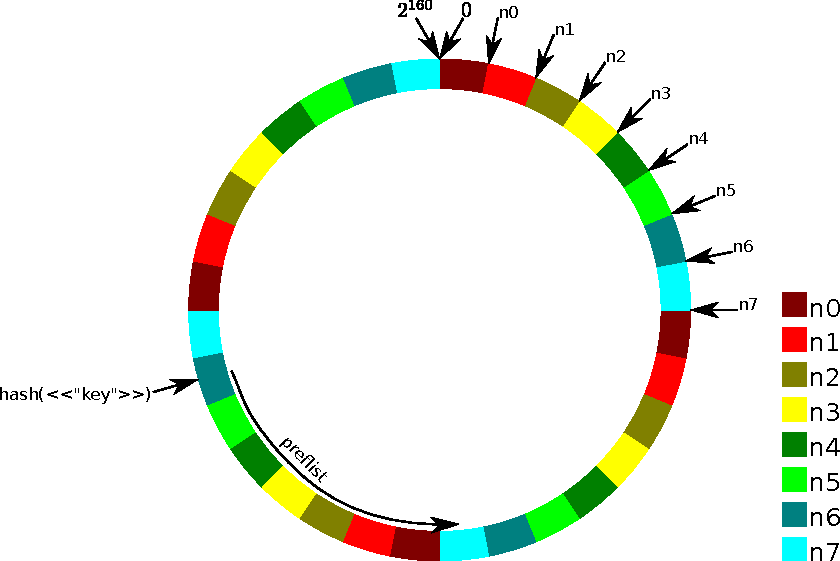
\includegraphics[width=\textwidth]{consistent_hashing_example}
\caption[Consistent Hashing Example]{Consistent Hashing Example.
	Ring with 32 partitions and 8 nodes.}
\label{fig:chash_example}
\end{figure}


\section{Riak Core Lite} 
\label{sec:riak_core_lite}
Riak Core was extracted from the Riak key-value store to enable a simple creation of distributed decentralized systems.
In an attempt to streamline and modularize the concept \ac{RCL}\cite{RiakCoreLiteTeam2020} was created from Riak Core.
One of the biggest motivations to use \ac{RCL} as the system to integrate \ac{RS} with is the simplified structure and shaved off features which leads to a lower potential for complications and errors while still upholding the basic principles of the Dynamo architecture.
As \ac{RCL} is rather a framework for distributed systems than a complete key-value store it's main functionality is the coordination of the nodes in the cluster and navigation of the Consistent Hashing ring.
It does not handle the actual data transfer or replication and instead just returns a plan for the replication in form of a preference list.
The following sections contain an overview of the basic system components and how they interact given some core use cases.

\subsection{System Components}
As the \ac{RCL} System consists of over 40 erlang-modules this sections groups some modules into logical components.
Here the descriptions of the components are on a more abstract level to keep the concepts simple but still enable a discussion of basic system functionalities in \cref{sec:system_procedures}.

\subsubsection{Ring}
	The ring is a central concept in the Dynamo architecture and Consistent Hashing.
	We discussed \ac{RCL}'s implementation of Consistent Hashing and the ring model this component is based on in \cref{sec:riak_core_consistent_hashing}.
	In a cluster every member has its current view of the ring.
	There is only one ring installed per instance, which is only accessible and mutable by this component.
	The ring enables an assignment of keys to nodes and to create the preference list via Consistent Hashing.
	To this end the ring guarantees that for each virtual node at least $N$ predecessor virtual nodes are owned by distinct physical nodes.
	As node failures are assumed as transient in the Dynamo architecture downed nodes are not removed from the ring.
	Instead the Navigation component handles failed nodes by skipping them in the filtered preference list.
	An additional responsibility of the ring is to merge two divergent rings after a network partitioning is fixed.

\subsubsection{Navigation}
	The navigation component enables a user to find the node responsible for a key and creating preference lists.
	It offers to query different kinds of filtered and annotated preference lists.
	For optimization purposes it offers a read-only binary encoding of the current ring with faster access time and lower memory consumption.

\subsubsection{Claim}
	\label{sec:claim}
	Claim handles the rebalancing of the load to nodes when the cluster changes.
	It is used when nodes join, leave or are recognized as down, and when the ring is resized.
	Therefore it is also the entry point of those actions through a stage-plan-commit life cycle in which several changes are staged, the resulting change plan is checked, and the changes are applied to the ring.
	The algorithm keeps the guarantees of the preference list and the ring intact.
	A central aspect of load balancing is to diagonalize the nodes on the ring instead of periodically repeating the same pattern to avoid unfinished patterns at the end of the ring.

\subsubsection{VNode}
	In the context of \ac{RCL} a virtual node represents the combination of the index of the partition on the ring and the owning physical node.
	A member can be a distinct physical machine or an instance on a physical machine.
	Those cases are not distinguished by \ac{RCL} and have to be handle by the system administrator.
	In the component tasks are scheduled and requested at the responsible nodes in an attempt to avoid overloading.
	Those tasks include handling messages sent to the nodes and executing a data handoff to other nodes.
	The virtual node also acts as a behavior definition for those tasks and therefore as the entry point for the application logic when using \ac{RCL}.

\subsubsection{Handoff}
	The handoff implements the concept of transferring data a node previously owned to the node currently owning the keys the data belongs to.
	The handoff component is responsible for creating the connection, creating the correct handoff message and preparing the handoff state a node works on.

\subsubsection{Gossip}
	The gossip protocol is responsible to communicate state updates to other cluster members via a random method that ensures eventual consistency.
	Each node gets assigned tokens periodically.
	As long as a node has tokens it sends the ring to randomly chosen other nodes.
	The gossip component also detects when a ring version changed and triggers the reconciliation in the ring component.

\subsubsection{Eventhandler}
	The eventhandler component allows to install different eventhandlers like one that listens to ring updates.
	Eventhandlers are used by \ac{RCL} internally, however they are also intended to help tailoring the system to the application logic by implementing custom ones.
	Several components are listening to ring update events to trigger procedures.
	This includes starting and registering vnodes or triggering the gossip protocol.

\subsection{System Procedures}
\label{sec:system_procedures}
The system procedures we list here only show a subset consisting of the most basic operations to demonstrate functionality offered by \ac{RCL} and build a ground for comparison to the system adaptions implemented in this thesis.
Any procedure that changes the cluster state, e.g. member status or ring size, have to be applied by the claim's stage-plan-commit cycle which is not explicitly mentioned for those procedures.
In this lifecycle a number of changes is staged via the claimant and premarked in the corresponding place.
Before one can commit the changes, a plan has to be created (see Action \ref{action:plan}, \cref{fig:plan}) and checked if the results are the desired ones.
When committing scheduled changes all changes are applied and the new ring is installed (see Action \ref{action:commit}, \cref{fig:commit}).

\subsubsection{Start Cluster}
When starting the cluster all system processes are started.
This includes starting the ring management system, initializing all virtual nodes and starting the gossip protocol.
When no information about an existing ring can be found on the machine starting the cluster it is assumed this is a new cluster.
Otherwise the ring is installed and the members are queried.
For details see Action \ref{action:start_cluster}, \cref{fig:start_cluster}.

\subsubsection{Join Cluster}
A node in a singleton cluster can join the cluster of another node.
To this end the other node is queried for the remote ring and the membership status of the ring is computed locally.
The ring with the updated members list then is sent via the gossip protocol.
To actually make the new node an owner on the ring the changes have to be planned and committed.
There is no handoff from the joining node to the existing cluster, only in the other direction.
Thus, any keys already stored on the joining node are lost.
For details see Action \ref{action:join_cluster}, \cref{fig:join_cluster}.

\subsubsection{Leave Cluster}
A node can leave the cluster with a call to it's local instance.
This causes the status of the local node to be marked as leaving in the ring.
The new member status is then gossiped to other members in the cluster.
When the claim is executed the next time and the executing node has knowledge of the leaving status the node is not considered for ring ownership and removed.
Leaving is the only ring change that is not applied via the stage-plan-commit life-cycle.
For details see Action \ref{action:leave_cluster}, \cref{fig:leave_cluster}.

\subsubsection{Remove Node}
Removing a node from the cluster causes it to directly hand off all of its data to other nodes.
This leads to a handoff of any sections owned by this node and marking the node invalid.
The status change will lead to the node being excluded from the ring and marked invalid on the next reconciliation.
For details see Action \ref{action:remove_node}, \cref{fig:remove_node}.

\subsubsection{Navigate the Ring}
There are several ways of executing navigation tasks in \ac{RCL}.
Using only the ring one can
\begin{itemize}
	\item find the index of the node responsible for a given key (see Action \ref{action:ring_find_index_for_key}, \cref{fig:ring_find_index_for_key}),
	\item find all indices owned by the local node (see Action \ref{action:ring_find_indices_for_node}, \cref{fig:ring_find_indices_for_node}),
	\item find the node owning a given index (see Action \ref{action:ring_find_node_for_index}, \cref{fig:ring_find_node_for_index}),
	\item compute a simple preference list assuming all nodes are up for a given key (see Action \ref{action:ring_preference_list}, \cref{fig:ring_preference_list}).
\end{itemize}
Via the navigation one can achieve the same results via an optimized structure:
\begin{itemize}
	\item find the index of the section responsible for a given key (see Action \ref{action:chashbin_find_index_for_key}, \cref{fig:chashbin_find_index_for_key}),
	\item compute the position\footnote{The position of a section describes the index of the section on the ring starting from as opposed to the index resulting from the hash function.} of the section responsible for a given key(see Action \ref{action:chashbin_find_partition_index_for_key}, \cref{fig:chashbin_find_partition_index_for_key}),
	\item retrieve the node owning the given index (see Action \ref{action:chashbin_find_ring_index_for_key}, \cref{fig:chashbin_find_ring_index_for_key}),
	\item compute the preference list assuming all nodes are up for a given key (see Action \ref{action:chashbin_preference_list}, \cref{fig:chashbin_preference_list}).
\end{itemize}
Different kinds of active preference lists that only consider up nodes can be computed via the navigation component.
Those include
\begin{itemize}
	\item a plain preference list (see Action \ref{action:get_apl_locally}, \cref{fig:get_apl_locally}).
	\item a preference list in which nodes are annotated as primary or fallback node (see Action \ref{action:get_annotated_apl_locally}, Action \ref{action:get_annotated_apl_locally}).
	\item a preference list only containing primary nodes (see Action \ref{action:get_primary_apl_locally}, \cref{fig:get_primary_apl_locally}).
\end{itemize}

\subsubsection{Resize Ring}
A resize operation can be staged via the claim component.
The ring size must be a power of 2 as otherwise load balancing cannot be achieved.
When a resize is committed special precautions are taken when computing new ownership relations and handoffs to avoid too many unnecessary reassignments and data transfers.
For details see Action \ref{action:resize_ring}, \cref{fig:resize_ring}.

\subsubsection{Handoff}
Nearly all kinds of cluster changes lead to a necessary data transfer.
When such a cluster change is committed via the claim, an entry for scheduled handoffs is added in the updated ring.
The vnode periodically reads these entries and checks for new ones.
When it finds new handoff entries a handoff request is sent to the node handing off data.
When the node is ready to handoff its data a handoff process folding over all stored data items is started by the node.
For details see Action \ref{action:handoff}, \cref{fig:handoff}.


%!TEX root=../master_thesis.tex

\chapter{Random Slicing}
\label{ch:random_slicing}
In this chapter we introduce the concept of \ac{RS} in detail.
The first section looks at \ac{RS} purely as a partitioning algorithm without considering replication.
Following this we discuss some simple approaches to integrate replication with \ac{RS}.

\section{Partitioning Algorithm}
\label{sec:partitioning_algorithm}
Miranda et al. have proposed \ac{RS}\cite{Miranda2014} as an ``efficient and scalable data placement for large-scale storage systems''.
The motivation to develop yet another data placement algorithm were several shortcomings of existing approaches like Consistent Hashing, especially when the cluster configuration changes often or scales to a high number of nodes.
The goal for the system is to keep a good adaptivity and fairness when scaling a cluster while keeping look-up time and memory consumption low and supporting redundancy in the cluster.
\emph{Adaptivity} here means the ability to reconfigure the cluster without moving unnecessary data points stored on it.
\emph{Fairness} is defined as the ability to distribute data and requests to nodes according to their capacity.

The basic principle of \ac{RS} is to assign one or more sections on the unit interval $[0,1)$ to each node in the cluster such that
\begin{enumerate}
	\item no assigned sections overlap,
	\item the interval is assigned completely,
	\item the sum of length of all sections assigned to a given node is equal to its relative capacity with respect to the total cluster capacity.
\end{enumerate}
This basic functionality can be seen as another variant of Consistent Hashing\cite{Fritchie2018}.

In detail the system starts with an initial configuration of nodes $n_1,...,n_k$ with capacities $c_1,...,c_k$ and relative capacities
\[
	r_i = \frac{c_i}{\sum\limits_{j=1}^kc_j}.
\]
The unit interval is simply split into intervals of length $r_i$ and each node is assigned the respective section.
Whenever the cluster configuration changes, either by removing nodes, adding nodes or by changing the capacity of existing nodes, new relative capacities for all nodes are computed.
Using the current assignment map and the new relative capacities a \emph{gap collection} algorithm chooses which sections of the current mapping are split or completely reassigned.
The authors propose and examine two simple algorithms and a sorted variant for each.
They determine that the \emph{CutShift+Sorted} algorithm yields the best results with respect to keeping the number of new sections low, which is the biggest influence on memory consumption and lookup time.
This algorithm tries to release only complete intervals first and alternates between splitting at the start and at the end of sections if splits are necessary to get bigger gaps.
The sorted variant in addition assigns the nodes with the highest capacity to the largest gaps.

However, Scott Fritchie, the Riak developer who proposed using \ac{RS} with Riak Core\cite{Fritchie2018}, implemented a greedy algorithm\footnote{\url{https://github.com/basho/machi/blob/master/src/machi_chash.erl}} for a different project which minimizes data transferred between nodes when the cluster is changed, as data transfers over a distributed network can be a bottle neck\cite{Fritchie2018}.
Its pseudocode can be found in Algorithm \ref{alg:gap_collection}.
This algorithm starts with computing the signed difference of relative capacities (\cref{line:gap_collection_diffs1,line:gap_collection_diffs2,line:gap_collection_diffs3}).
Then, for each node with shrinking relative capacities gaps are collected greedily by iterating their sections and marking sections as unused until they meet the capacity difference (\cref{line:gap_collection_neg1,line:gap_collection_neg2,line:gap_collection_neg3,line:gap_collection_neg4,line:gap_collection_neg5,line:gap_collection_neg6,line:gap_collection_neg7,line:gap_collection_neg8,line:gap_collection_neg9,line:gap_collection_neg10,line:gap_collection_neg11,line:gap_collection_neg12,line:gap_collection_neg13}).
At most one section is split per node, which happens if the currently viewed section is larger than the remaining difference.
The created gaps are then greedily assigned to the nodes with a growing relative capacity in the same manner (\cref{line:gap_collection_pos1,line:gap_collection_pos2,line:gap_collection_pos3,line:gap_collection_pos4,line:gap_collection_pos5,line:gap_collection_pos6,line:gap_collection_pos7,line:gap_collection_pos8,line:gap_collection_pos9,line:gap_collection_pos10,line:gap_collection_pos11,line:gap_collection_pos12,line:gap_collection_pos13,line:gap_collection_pos14,line:gap_collection_pos15}).
Therefore, at most one gap is split per node for the same reasons.
Now that the complete interval is assigned, neighboring sections with the same owner are merged into one section (\cref{line:gap_collection_merge}).

\begin{algorithm}
\caption{Gap Collection}
\label{alg:gap_collection}
\SetKwData{Sections}{sections}
\SetKwData{Capacities}{capacities}
\SetKwData{OldCapacities}{old\_capacities}
\SetKwData{CapacityDiff}{capacity\_diff}
\SetKwData{RelCapacities}{rel\_capacities}
\SetKwData{Unowned}{unowned}
\SetKwFunction{GetOwner}{GetOwner}
\SetKwFunction{SetOwner}{SetOwner}
\SetKwFunction{Length}{Length}
\SetKwFunction{Split}{Split}
\SetKwFunction{Append}{Append}
\SetKwFunction{Replace}{Replace}
\SetKwFunction{NextUnowned}{NextUnowned}
\SetKwFunction{MergeSameNeighbors}{MergeSameNeighbors}
\KwData{List of sections \Sections, List of new relative capacities \Capacities}
\KwResult{New assignment of sections to nodes \Sections}
\For{$s\in\Sections$}{
 $\OldCapacities[\GetOwner{s}] \leftarrow \OldCapacities[\GetOwner{s}] + \Length{s}$
}
\For{$\{o, c\}\in\Capacities$}{\label{line:gap_collection_diffs1}
 $\CapacityDiff[o]\leftarrow c - \OldCapacities[o]$\;\label{line:gap_collection_diffs2}
}\label{line:gap_collection_diffs3}
\For{$s\in\Sections$}{
 $o \leftarrow \GetOwner{s}$\;
 $d \leftarrow \CapacityDiff[o]$\;
 $l\leftarrow \Length{s}$\;
 \If{$d < 0$}{\label{line:gap_collection_neg1}
  \If{$|d|\leq l$}{\label{line:gap_collection_neg2}
   $\{s_1,s_2\}\leftarrow \Split{s, l - |d|}$\;\label{line:gap_collection_neg3}
   $s_2\leftarrow\SetOwner{$s_2$, \Unowned}$\;\label{line:gap_collection_neg4}
   $\Sections\leftarrow\Replace{\Sections, s, ($s_1$, $s_2$)}$\;\label{line:gap_collection_neg5}
   $\CapacityDiff[o]\leftarrow 0$\;\label{line:gap_collection_neg6}
  }\label{line:gap_collection_neg7}
  \If{$|d| > l$}{\label{line:gap_collection_neg8}
   $s\leftarrow\SetOwner{s, \Unowned}$\;\label{line:gap_collection_neg9}
   $\Sections\leftarrow\Replace{\Sections, s, s}$\;\label{line:gap_collection_neg10}
   $\CapacityDiff[o]\leftarrow d + l$\;\label{line:gap_collection_neg11}
  }\label{line:gap_collection_neg12}
 }\label{line:gap_collection_neg13}
}
\For{$(o,d)\in\CapacityDiff$}{
 \While{$d > 0$}{\label{line:gap_collection_pos1}
  $s \leftarrow \NextUnowned{\Sections}$\;\label{line:gap_collection_pos2}
  $l\leftarrow \Length{s}$\;\label{line:gap_collection_pos3}
  \If{$|d|\leq l$}{\label{line:gap_collection_pos4}
   $\{s_1,s_2\}\leftarrow \Split{s, l - |d|}$\;\label{line:gap_collection_pos5}
   $s_1\leftarrow\SetOwner{$s_1$, o}$\;\label{line:gap_collection_pos6}
   $\Sections\leftarrow\Replace{\Sections, s, ($s_1$, $s_2$)}$\;\label{line:gap_collection_pos7}
   $\CapacityDiff[o]\leftarrow 0$\;\label{line:gap_collection_pos8}
  }\label{line:gap_collection_pos9}
  \If{$|d| > l$}{\label{line:gap_collection_pos10}
   $s\leftarrow\SetOwner{s, o}$\;\label{line:gap_collection_pos11}
   $\Sections\leftarrow\Replace{\Sections, s, s}$\;\label{line:gap_collection_pos12}
   $\CapacityDiff[o]\leftarrow d - l$\;\label{line:gap_collection_pos13}
  }\label{line:gap_collection_pos14}
 }\label{line:gap_collection_pos15}
}
$\Sections \leftarrow \MergeSameNeighbors{\Sections}$\;\label{line:gap_collection_merge}
\Return \Sections\;
\end{algorithm}

Determining the node a given key belongs to can be achieved by applying a hash function to the key and mapping the hash space to the unit interval.
This is done both for storing and retrieving data.
Redundancy can be achieved by different strategies and only some simple solutions are given in the original paper.
We discuss some simple approaches to solving the redundancy problem in Section \ref{sec:replication_placement_strategy}.

In addition to the description of their approach, Miranda et al.\cite{Miranda2014} conducted an analysis on different data placement strategies including two variants of Consistent Hashing in a simulated environment to compare them with respect to fairness, memory usage, lookup time, and adaptivity.
The summary of their qualitative results can be found in Table \ref{tab:random_slicing_analysis} taken from the original paper\cite{Miranda2014}.
As one can see \ac{RS} performs better than the other strategies when looking at each of their weak points.
It is however important to note that the analysis was done for large-scale system together with high redundancy for which some of the strategies were not developed.
As mentioned before the adaptivity can be improved by using a different gap collection algorithm at the cost of memory usage and lookup time.

Figure \ref{fig:random_slicing_example} shows an example of \ac{RS} with Fritchie's gap collection algorithm .
In this example the unit interval is interpreted as a ring running clockwise with the 0/1 point at the top like in Consistent Hashing to make a comparison easier.
The used nodes all have the same capacity.
In the example each ring represents a configuration of the cluster, with the most outward ring being the initial and the inner ring being the final configuration.
Initially 4 nodes get assigned a quarter of the ring each.
In the second configuration one node is added.
The new node takes an equal part of each existing section such that each node owns a fifth of the interval.
Two new nodes are added in the next step.
One can see, that some small intervals are reassigned completely and some are split.
The transition is from 7 to 10 nodes in which one can easily see the mechanism of splitting gaps while assigning nodes.
The fact that gaps are only assigned to new nodes implies that there are no transfers of data between existing nodes.
This shows that the amount of transferred data is optimal for each reconfiguration.

\begin{figure}
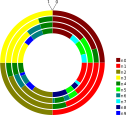
\includegraphics[width=\textwidth]{random_slicing_example}
\caption[Random Slicing example]{Random Slicing example scaling from 4 to 5 to 7 to 10 nodes with homogeneous capacity.}
\label{fig:random_slicing_example}
\end{figure}

\begin{table}
\begin{tabularx}{\textwidth}{|l|X|X|X|X|}
\hline
Strategy & Fairness & Memory usage & Lookup time & Adaptivity\\
\hline
\emph{Consistent Hashing (fixed)} & Poor & High & Moderate & Good\\
\emph{Consistent Hashing (adapt.)} & Moderate & High & High & Poor\\
\emph{Redundant Share} & Good & Low & Very High & Good\\
\emph{$\text{RUSH}_\text{P}$} & Poor & Low & Very High & Very Good\\
\emph{$\text{RUSH}_\text{R}$} & Good for low number of replicas & Low & Low &Very Good\\
\emph{$\text{RUSH}_\text{T}$} & Good & Low & Very High & Very Good\\
\emph{Random Slicing} & Good & Low & Low & Good\\\hline
\end{tabularx}
\caption[Qualitative analysis of different data placement strategies]{Qualitative analysis of different data placement strategies. Reprinted from \cite{Miranda2014}.}
\label{tab:random_slicing_analysis}
\end{table}

\section{Replication Placement Strategy}
\label{sec:replication_placement_strategy}
After the initial node to store a data block by its key is chosen through hashing on the intervals created by \ac{RS}, additional $N-1$ copies have to be distributed to $N-1$ distinct physical nodes.
For the correctness of \acp{RPS} it is assumed that the system configuration is correct, which means at times of operational states there are $n \geq N$ physical nodes in the cluster and $R \leq W \leq N$.
The \ac{RPS} should return a preference list of at least $N$ nodes, where the initial node is the head and the tail consists of nodes where replicas are stored in descending preference.

Load balancing between all nodes should be achieved at least asymptotically such that it gets closer to the ideal value when the ratio of replicas to nodes in the cluster $\frac{N}{n}$ gets smaller.
Considering only the primary replica, i.e. the head of the preference list, a placement strategy should always achieve perfect load balancing for a uniform distribution of data.
The ideal case is that for relative capacities $c_1,..,c_n$ of the nodes their relative load $l_i$ should be equal to the capacity $c_i$.
The relative capacity of node $n_i$ with weight $w_i$ is $c_i = \frac{w_i}{\sum_{j=1}^{n}w_j}$.
The relative load of node $n_i$ after $k$ keys have been distributed and $k_i$ keys are stored on $n_i$ is $l_i = \frac{k_i}{Nk}$.

To support the gossip protocol and local functionality of \ac{RCL} the replication strategy must not use a central server or other communication between the nodes.
The result should only be based on the current local view.
If two local views are the same, the preference list should be the same, i.e be deterministic.


\subsection{Random Replication}
This simple approach uses the outputs of a random uniform function as keys until $N$ distinct physical nodes are hit.
To achieve the same preference list for the same partitioning across all nodes the random function is seeded with the initial key.
A pseudo code  version of the algorithm is shown in Algorithm \ref{alg:trivial}.
Random Replication was chosen by Miranda et al. as the replication strategy in the analysis of \ac{RS}\cite{Miranda2014}.
Initially Brinkmann et al. mention this approach as a motivation for Redundant Share\cite{Brinkmann2007}.
Theoretical results showing non-optimal capacity usage in a heterogeneous system seem to have a neglectable impact on load balancing according to the simulations done by Miranda et al.

\begin{algorithm}
\caption{Trivial Replication}
\label{alg:trivial}
\SetKwData{Preflist}{preflist}
\SetKwData{Secs}{secs}
\SetKwFunction{GetNode}{GetNode}
\SetKwFunction{Length}{Length}
\SetKwFunction{Append}{Append}
\SetKwFunction{Rand}{Rand}
\KwData{List of sections \Secs, number of required replicas $N$, key of data to be replicated $k$}
\KwResult{\Preflist of at least length $N$}
$i \leftarrow 0$\;
$\Preflist \leftarrow \emptyset$\;
\While{\Length{\Preflist} $< N$}{
	$r \leftarrow \Rand{i, k}$\;
	\If{\GetNode{\Secs, $r$}$\notin$ \Preflist}{
				\Append{\Preflist, \GetNode{\Secs, $r$}}\;
	}
	$i \leftarrow i + 1$\;
}
\end{algorithm}

\subsubsection{Worst Case Runtime}
Since the process of finding nodes to store replicas on is random the worst case is that not enough nodes are hit after a finite number of steps and the replication algorithm does not terminate.
However, this is highly improbable.
We show this by computing probabilities of a fixed node with relative capacity $c$ being picked after $k$ steps.
To this end we model a random experiment with the geometric distribution.
Each independent trial has a probability of $c$ that the fixed node is drawn and $1-c$ that it is not drawn.
Therefore the probability to draw the node after exactly $k$ steps is
\[
	Pr(X=k)=(1-c)^{k-1}c,
\]
the expected value for $k$ is
\[
	E(X)=\frac{1}{c}
\]
and the probability to draw the node after at most $k$ steps is
\[
	Pr(X\leq k)=\sum\limits_{i=1}^{k}(1-c)^{i-1}c=c\sum\limits_{i=0}^{k-1}(1-c)^{i}=c\frac{(1-c)^0-(1-c)^{k}}{1-(1-c)}=1-(1-c)^k.
\]
Solving the inequality $Pr(X\leq k) = 1-(1-c)^k \geq p$ for $k$ yields
\[
	k \geq \log_{1-c}(1 - p)
\]
and therefore the minimal value fulfilling this inequality is
\[
	k=\lceil\log_{1-c}(1 - p)\rceil
\]

To further illustrate these values first we choose three different scenarios and compute $E(X)$, $Pr(X\leq k)$ for $k\in\{i\cdot n\mid i\in\{1,...,5\}\}$, and the minimal values for $k$ such that $Pr(X\leq k)\geq 0.95$ and $Pr(X\leq k)\geq 0.99$.
The first scenario $S_1$ is derived from the example shown in \cref{fig:random_slicing_example}.
Here there are 10 homogeneous nodes with the same capacity.
Therefore $n_1=10$ and $c_1=0.1$.
The second scenario $S_2$ is motivated by a high scaling with 1000 homogeneous nodes.
Therefore $n_2=1000$ and $c_2=0.001$.
The last scenario $S_3$ represents a heterogeneous system in which we consider a node with only a tenth of the average capacity.
We choose $n_3=10$ and $c_3=0.01$

The numbers for those scenarios are shown in \cref{tab:probabilities}.
An interesting aspect is that for the homogeneous scenarios all values appear to scale with the number of nodes.
The number of steps needed to guarantee that a given node is chosen with a specific probability also scales with the ratio of the actual capacity of the node to the average capacity.
While these results are not surprising when looking at the equation we intend to give an easier understanding with those examples.


\begin{table}
\begin{tabularx}{\textwidth}{|l|X|X|X|X|X|X|X|X|}
\hline
Scenario & $E(X)$ & $Pr_{1n}$ & $Pr_{2n}$ & $Pr_{3n}$ & $Pr_{4n}$ & $Pr_{5n}$ & $k_{0.95}$ & $k_{0.99}$\\\hline
$S_1$ & 10 & 0.651 & 0.878 & 0.958 & 0.985 & 0.995 & 29 & 44\\
$S_2$ & 1000 & 0.632 & 0.865 & 0.950 & 0.982 & 0.993 & 2994 & 4603\\
$S_3$ & 100 & 0.182 & 0.331 & 0.453 & 0.552 & 0.634 & 298 & 458\\
\hline
\end{tabularx}
\caption[Example Probabilities with Random Replication]{Example Probabilities with Random Replication. Shows expected value for $k$, probabilities that the node is chosen within a given number of steps and number of steps needed to be chosen with a given probability.}
\label{tab:probabilities}
\end{table}


\subsubsection{Example}
Using the final ring from the example in Figure \ref{fig:random_slicing_example} and the key $0.345$ the resulting preference list is \lstinline![n1,n8,n4,n9,n5,n2,n7,n6,n0,n3]!.
The random algorithm used to create the random keys is Erlang's implementation of the Xorshift116 generator combined with the StarStar scrambler\cite{Blackman2018}.

\subsubsection{Discussion}
Using random replication leads to near perfect load balancing according to simulations by Miranda et al\cite{Miranda2014}.
It is highly unlikely that the same node is drawn over and over when the ratio of available nodes to required nodes is high enough and therefore the runtime can be expected to be nearly linear in the number of required nodes.
Since the random function is seeded with the primary key, the placement on the unit interval of replica candidates is deterministic for each key.
Therefore after a cluster reconfiguration not all replica placements have to be recomputed as they can be moved to the node now responsible for that section.
Recomputation is only necessary if the positions of two replicas are owned by the same node after a reconfiguration and therefore the preference list not having enough distinct members.

\subsection{Ring Rotation}
Another approach has the intention of keeping Riak Core's ring structure and making use of it.
A pseudo code version of this algorithm is shown in  Algorithm \ref{alg:ring_rotation}.
The ring rotation is visualized in Figure \ref{fig:ring_rotation}.
Its idea is to stepwisely rotate the ring counter-clockwise, or from another perspective, the key clockwise, by the lengths of its sections and use the original hash value to create the preference list.
The aim of this approach is to achieve load balancing by considering the lengths of the sections.
However, there is a possibility that after a whole rotation of the ring less than $N$ nodes are in the preference list.
To overcome this, in the $i$-th rotation the sections are split into $2^i$ subsections and therefore the rotation step lengths get shorter (\cref{line:rotation_step}).
This leads to smaller segments that were previously skipped by rotating by a bigger length to be added to the preference list.
Since the rotation of the subsections leads to querying the same key value multiple times, a small optimization would be to skip those values (\cref{line:rotation_skip}).
This is done by rotating the ring by $\frac{1}{2^i}$ of the original length once to offset the value, then rotate it $2^{i-1}-1$ times by $\frac{1}{2^{i-1}}$  of the original length and finally the offset is reverted without querying the ring.
Implementation wise instead of the ring being rotated counter-clockwise the key is rotated around the ring clockwise.

\begin{algorithm}
\caption{Rotation for each segment}
\label{alg:ring_rotation}
\SetKwData{Preflist}{preflist}
\SetKwFunction{Length}{Length}
\SetKwFunction{GetNode}{GetNode}
\SetKwFunction{GetLength}{GetLength}
\SetKwFunction{Append}{Append}
\SetKwFunction{SubList}{SubList}
\KwData{Mapping of ranges to nodes $m$, number of required replicas $N$, index of data to be replicated $k$}
\KwResult{\Preflist of at least length $N$}
$i \leftarrow 0$\;
$\Preflist \leftarrow \emptyset$\;
$m \leftarrow \Append{\SubList{m, \GetNode{k}, \Length{m}}, \SubList{0, \GetNode{k}}}$\;
\While{\Length{\Preflist} $< N$}{
	\For{$s \in m$}{
		$step \leftarrow \GetLength{s}\cdot 2^{-i}$\;\label{line:rotation_step}
		\tcp{One step to offset the key}
		$k \leftarrow (k + step)$\;
		\If{$k \geq 1.0$}{
			$k \leftarrow k - 1.0$\;
		}
		\If{\GetNode{$m$, $k$}$\notin$ \Preflist}{
			\Append{\Preflist, \GetNode{$m$, $k$}}\;
		}
		\tcp{Skip previously visited indices}
		\For{$j \leftarrow 1$ \KwTo $2^{i-1}-1$}{
			
			$k \leftarrow (k + 2\cdot step)$\;\label{line:rotation_skip}
			\If{$k \geq 1.0$}{
				$k \leftarrow k - 1.0$\;
			}
			\If{\GetNode{$m$, $k$}$\notin$ \Preflist}{
				\Append{\Preflist, \GetNode{$m$, $k$}}\;
			}
		}
		\tcp{One step to change offset to first index of the next node without lookup}
		$k \leftarrow (k + step)$\;
		\If{$k \geq 1.0$}{
			$k \leftarrow k - 1.0$\;
		}
	}
	$i \leftarrow i + 1$\;
}
\Return{\Preflist}
\end{algorithm}

\begin{figure}
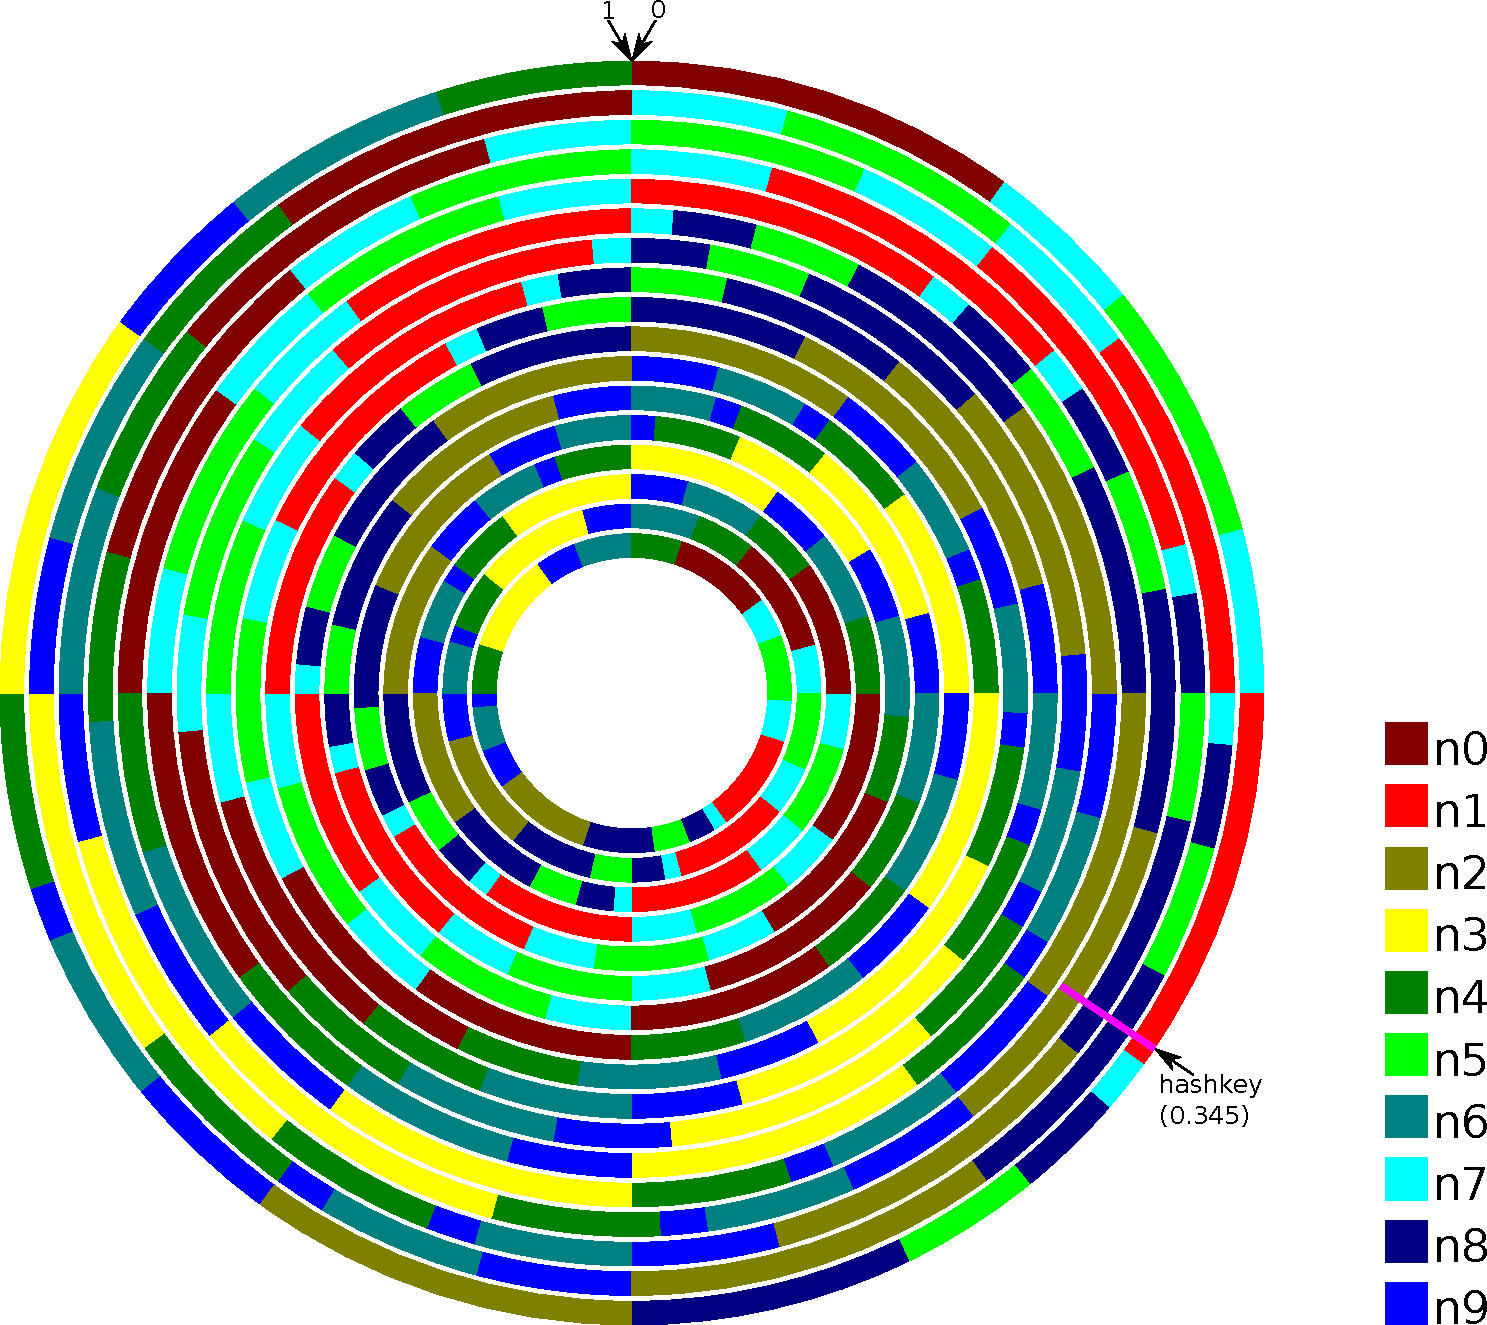
\includegraphics[width=\textwidth]{random_slicing_rotation}
\caption[Visualization of the ring rotation replication]{Visualization of the ring rotation replication.
n0...n9 are the physical nodes.
The ring is rotated counterclockwise by the length of each section.
From the outer to the inner ring each rotation step is shown.
}
\label{fig:ring_rotation}
\end{figure}

\subsubsection{Correctness}
The algorithm is seen as correct if it constructs a preference list of $N$ distinct physical nodes for any correct system configuration with $n\geq N$ nodes.
The maximum rotation length will be eventually smaller than the shortest section.
Therefore after a finite amount of rotations each section on the ring will be queried which leads to a preference list containing each physical node.
Since the system configuration is assumed to be correct the preference list contains at least $N$ distinct physical nodes.

\subsubsection{Worst Case Runtime}
In the worst case $N$ is equal to the number of distinct physical nodes and the ring actually has to rotate the maximum number of rounds.
 Let $s$ be number of segments, $l_{max}$ length of the largest segment, $l_{min}$ length of the shortest segment.
Starting with round $i=0$ the number of steps per round is $r(i) = 2^i\cdot s$
Therefore the total number of steps for $k$ rounds is
\[
\sum\limits_{i=0}^{k-1}2^i\cdot s = s\cdot \sum\limits_{i=0}^{k-1}2^i = s\cdot\frac{1-2^k}{1-2} = (2^k - 1)\cdot s
\]
and the number of rounds in the worst case is
\begin{align*}
\frac{l_{max}}{2^k} &\leq l_{min}\\
\frac{l_{max}}{l_{min}} &\leq 2^k\\
k &\geq \log_2(\frac{l_{max}}{l_{min}})\\
k &= \lceil \log_2(\frac{l_{max}}{l_{min}}) \rceil.
\end{align*}

\subsubsection{Load Balancing}
\ac{RS} guarantees load balancing for the primary copy of a data item.
Looking at Figure \ref{fig:ring_rotation} one can see that sections owned by the same node do overlap from one rotation step to another.
This complicates a quantitative analysis of load balancing and we have to rely on simulated data for quantitative results.
However, the overlaps intuitively lead to an imperfect load balancing as the overlapping section is unused in all rotation steps but the first it appears in.

\subsubsection{Example}
Using the example from Figure \ref{fig:ring_rotation} and hash key $0.345$, the resulting preference list is \lstinline![n1,  n8, n2, n9, n4, n3, n6, n0, n5, n7]!.
To achieve a preference list for $N=3$, 3 rotation steps are necessary for that key.
To achieve a preference list for $N=10$, 15 rotation steps are necessary for that key.

\subsubsection{Discussion}
From the initial look the ring rotation replication seems to be sub-optimal both with respect to the expected runtime as well as the expected load balancing.
Since the rotations are based on the length of sections a reconfiguration of the cluster leads to a total rearrangement of replica placements.
Overall this approach does not look like a promising solution to the placement of replicas.

\subsection{Ring Jumping}
Similar to the ring rotation approach ring jumping  makes use of the original ring structure.
A pseudo code version of the algorithm is shown in Algorithm \ref{alg:ring_jumping} and a visualization can be seen in Figure \ref{fig:ring_jumping}.
However, instead of rotating the ring in the order of its sections it is rotated by the length of the section the key currently belongs to.
This is repeated until $N$ distinct physical nodes are added to the preference list.

\begin{algorithm}[H]
\caption{Ring Jumping}
\label{alg:ring_jumping}
\SetKwData{Preflist}{preflist}
\SetKwData{Secs}{secs}
\SetKwFunction{GetLength}{GetLength}
\SetKwFunction{GetNode}{GetNode}
\SetKwFunction{Append}{Append}
\KwData{List of sections \Secs, number of required replicas $N$, index of data to be replicated $k$}
\KwResult{\Preflist of at least length $N$}
$\Preflist \leftarrow \emptyset$\;
\While{\Length{\Preflist} $< N$}{
	$k \leftarrow k + \GetLength{\Secs, k}$\;
	\If{$k \geq 1.0$}{
				$k \leftarrow k - 1.0$\;
	}
	\If{\GetNode{\Secs, $k$}$\notin$ \Preflist}{
				\Append{\Preflist, \GetNode{\Secs, $k$}}\;
	}
}
\end{algorithm}

\begin{figure}
\centering
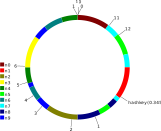
\includegraphics[width=0.5\textwidth]{random_slicing_jumping}
\caption{Ring Jumping}
\label{fig:ring_jumping}
\end{figure}

\subsubsection{Correctness}
Assume that the key is rotated around the ring such that it is within the initial section again for the first time.
If it is at its exact starting place then the sum of lengths of sections it hit is 1, which can only be the case if it visited every section and therefore every physical node was added to the preference list.
Otherwise, the starting place of the key for the next rotation is less than the initial one.
Then there is a chance that segments that where skipped before are now added to the preference list.
This is done until the key is at an initial position between the start of the starting section and its offset by the length of the shortest section.
Then it is guaranteed that every section is visited in the following rotation.

\subsubsection{Worst Case runtime}
The worst case occurs when the initial key is at the right edge of the longest segment and the shortest segment has to be visited.
Additionally only the shortest segment is not visited and therefore the position offset for each round is minimal.
Let $s$ be number of segments, $l_{max}$ length of the largest segment, $l_{min}$ length of the shortest segment.
Assume that only the shortest segment is not visited.
Therefore the start index of the next round moves by $l_{min}$: $s_{i+1} = s_{i} - l_{min}$.
The shortest segment is guaranteed to be hit in round $k$ if $s_k \leq l_{min}$.
So the number of rounds needed is $\lceil\frac{l_{max}}{l_{min}}\rceil$ and the number of steps needed is $s\cdot\lceil\frac{l_{max}}{l_{min}}\rceil$.

\subsubsection{Load Balancing}
Analyzing load balance properties of jumping approach qualitatively is complicated by the influence of section lengths and order.
Assuming equal section length and distribution this approach is equivalent to Riak Core's \ac{RPS} as the $N$ next sections are chosen by definition.
Abstracting from this special case the load on a section is expected to scale with its relative size.
However, the actual numbers need to be determined experimentally in a simulated environment.

\subsubsection{Example}
In Figure \ref{fig:ring_jumping} one can see how the $10$ nodes are selected for the preference list for the key $0.345$.
This results in \lstinline![n1, n8, n2, n9, n6, n3, n0, n7, n5]!.
Defining the \emph{efficiency} of the approach by the ratio of number of selected nodes to number of queries shows an efficiency of $100\%$ for the first six nodes.
To get a complete preference list with $10$ nodes 13 queries are required resulting in an efficiency of $76.9\%$.

\subsubsection{Discussion}
While not having the best expected runtime and unknown load balancing after the initial look this approach still has the potential to prove itself as a feasible solution for the replica placement in simulations.
As the approach is derived from Riak Core's algorithm it may also make visualizing differences easier.
One drawback of the approach is the dependency on the length and order of sections.
This creates a need to recompute the replica placements for any cluster reconfiguration and a repair operation.
If this is not done, keys can be lost with each cluster change.

%!TEX root=../master_thesis.tex

\chapter{Riak Core Lite and Random Slicing}
This chapter covers how the architecture and behavior of \ac{RCL} was changed while replacing Consistent Hashing with \ac{RS}.
First we give an explicit recapture of the responsibilities and guarantees of Consistent Hashing in \ac{RCL}, how \ac{RS} compares in those aspects, and what open problems directly follow from this comparison.
Analogous to Section \ref{sec:riak_core_lite} the next sections contain changed and new components as well as system actions that changed.

\section{Comparing Consistent Hashing and Random Slicing}
In \ac{RCL} Consistent Hashing provides a homogeneous partitioning of the ring.
Together with the claim algorithm it guarantees that for each partition the $N$ successor partitions are owned by $N$ distinct nodes if there are enough nodes in the cluster.
This enables a simple and fast computation of the preference list.
The indices on the ring are fixed unless a special resize operation is executed.
We visualize the difference between the ring structures in Figure \ref{fig:chash_and_rslicing}.

On the other hand \ac{RS} partitions the ring into dynamic sections.
It does not give a guarantee on the order of owners and therefore does not enable a simple and fast computation of the preference list.
Since the partitioning of the ring happens dynamically there is no resize operation.

From this one can conclude that open problems are the computation of the preference list and if there are changes that originally happened during the resize operation and are still relevant and therefore need to be applied elsewhere.
We discuss solutions for the computation of the preference list in Section \ref{sec:replication_placement_strategy} and other open problems are discussed in the appropriate places in the following sections.

\begin{figure}
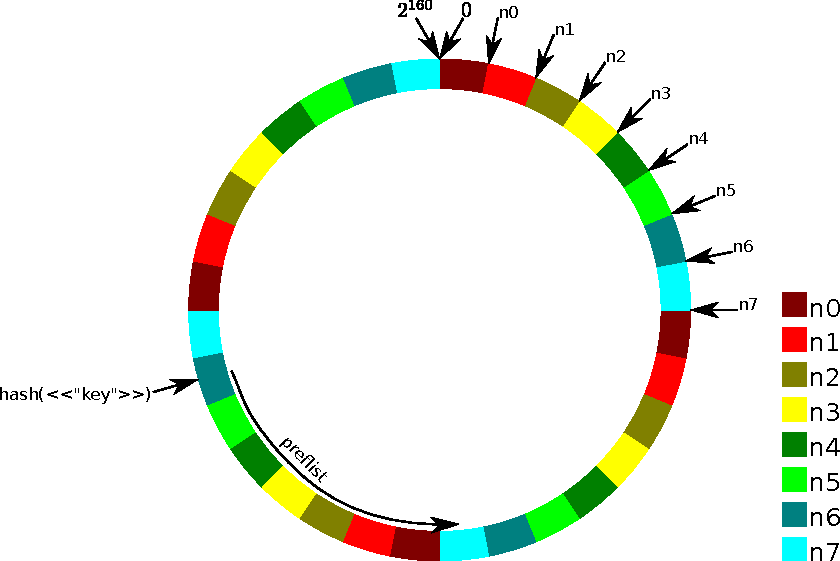
\includegraphics[width=0.5\textwidth]{consistent_hashing_example}
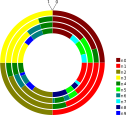
\includegraphics[width=0.5\textwidth]{random_slicing_example}
\caption[Side by Side Comparison of Consistent Hashing and Random Slicing]{Side by Side Comparison of Consistent Hashing and Random Slicing. On the left one can see the homogeneously partitioned Consistent Hashing ring while on the left one can see the dynamic changes in the \ac{RS} ring.}
\label{fig:chash_and_rslicing}.
\end{figure}


\section{Changed Components}
In this section we explain how the components listed in Section \ref{sec:replication_placement_strategy} were changed during the integration of \ac{RS} both with respect to their responsibilities as well as their basic functionality.
Any component that is not mentioned in this section was left unchanged or only changed on a technical level.

\subsection{Ring}
On an abstract level there are only minor changes in the ring component.
The model of the ring changed to that of \ac{RS} and therefore the computation of the preference list is now solely relying on the navigation component.
As the indices are not fixed in the new ring model the ring reconciliation algorithm had to be overhauled and relies now on choosing the most up-to-date ring and adding all missing members to it via the \ac{RS} algorithm.

\subsection{Navigation}
\label{sec:navigation_rslicing}
The navigation component had to be reworked almost completely.
First of all, the Consistent Hashing model at its core was replaced by an adaptation of Scott Fritchie's \ac{RS} implementation (see Sec \ref{sec:partitioning_algorithm}).
From that it directly follows, that the preference list cannot be computed by iterating over the successor nodes in the ring.
Instead the component uses the \acp{RPS} we present in Section \ref{sec:replication_placement_strategy}.
This also leads to strong restrictions on the use of the optimized read-only structure this component uses as it cannot be used to compute the preference list.

\subsection{Claim}
As the core component of the claim component the claim algorithm is obsolete as load balancing on the ring is directly achieved by Random Slicing.
Since the claim component is also responsible for the stage-plan-commit life cycle it still stays relevant and is the entry point for changes to the ring.
Instead of applying the claim algorithm in the commit phase the new ring is computed by using \ac{RS} with the old ring and new cluster configuration.
Through this it is assured the new guarantees given by the \ac{RS} model are fulfilled in the actual ring.


\section{Changed System Procedures}
In this chapter we explain the changes we made to the system procedures while integrating \ac{RS} with Riak Core.
Procedures that are mentioned in Section \ref{sec:system_procedures} but do not appear in this section are not changed significantly.

The system still uses the stage-plan-commit life-cycle for cluster changes. The stage phase has not changed as the cluster changes are still marked in the ring and gossiped to all members.
However, in the commit phase the updated ring is now computed by simply applying \ac{RS} to the old ring with the new member configuration.

\subsection{Leave Cluster}
The procedure of leaving the cluster remains unchanged in the most parts.
However, the leaving node is now actually removed from the ring on the next update-ring-event instead of the next claim execution.

\subsection{Navigate the Ring}
As we mentioned in Section \ref{sec:navigation_rslicing} the navigation component only offers reduced functionality with the optimized binary structure.
The removed functionalities include computing the preference list via that structure.
It now uses the ring model directly.
This does not restrict the functionalities of the navigation component but it may have a negative impact on the performance.
Other procedures navigating the ring were only changed in the aspect that they now use the \ac{RS} ring model together with the new replication placement algorithms.

\subsection{Resize Ring}
As there is no fixed ring size and the ring structure is changed with every cluster change there is no explicit resize operation anymore.
In the current state of the system any optimization and corner case handling in the handoff and ring update procedures during a resize operation is lost.

\subsection{Handoff}
While the actual execution of the handoff from the old owner of an index to the new owner has not changed the preparation of the handoff has changed significantly.
As the ring has no fixed indices anymore it has to be assured that there are virtual nodes running for all old and new indices.
This is achieved by computing a handoff-ring from the old and new ring that includes all indices of both rings and each index is owned by the onwer that would own it in the old ring.
This procedure is visualized with an example in Figure \ref{fig:handoff_ring}.
From this handoff ring the correct virtual nodes are running and can start the handoff procedure as usual.
When there are two neighboring sections owned by the same physical node the sections are merged on the next ring-update-event.

\begin{figure}
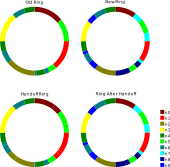
\includegraphics[width=\textwidth]{handoff_ring}
\caption[Handoff Ring]{Handoff Ring. First the indices of the old and new rings are merged and then assigned to the old owners. After the handoff the new ring results.}
\label{fig:handoff_ring}
\end{figure}

%!TEX root=../master_thesis.tex
\chapter{Evaluation}
In this chapter we present the evaluation of the integration of \ac{RS} with \ac{RCL}.
First we present hypotheses on how the adapted system will perform with respect to different aspects compared to the current \ac{RCL} implementation.
Following we explain which tools we use and how the environment and benchmarked systems are configured.
After this we explain which metrics we plan to take from the benchmark data to test our hypotheses.
Closing this chapter we show and interpret the results with respect to our hypotheses.

\section{Hypotheses}
In this section we present and reason about the hypotheses we test in this evaluation.
The hypotheses are based on the theoretical thoughts presented in \cref{ch:background,ch:random_slicing}.

One variant in the implementation of \ac{RS} in \ac{RCL} having a big impact is the replication placement algorithm.
The aspects most interesting to examine in this evaluation are the impact on load balancing and throughput.
From the initial discussion Random Replication seems to be the most promising approach of the simple ones in those aspects.
Therefore we postulate the following hypotheses:
\begin{hypothesis}
\label{hyp:replication_load_balancing}
	The average divergence from optimal load balancing over all nodes for Random Replication is less than for Ring Rotation or Ring Jumping.
\end{hypothesis}
\begin{hypothesis}
\label{hyp:replication_throughput}
	With Random Replication the system has a higher average throughput than with Ring Rotation or Ring Jumping.
\end{hypothesis}

In the following when we speak of \ac{RS} we mean \ac{RS} with the best performing of the replication placement algorithms.
From Miranda et al.'s analysis of \ac{RS}\cite{Miranda2014} it follows that it performs better than the original Consistent hashing both with respect to load balancing as well as performance.
However, \ac{RCL} uses an implementation of Consistent Hashing that is quite different from the original one and the system architecture is built around that version.
Additionally, in the scope of this thesis \ac{RS} was integrated with \ac{RCL} in a prototyping manner as a proof of concept and misses much architectural planning and loses a lot of optimization.
For those reasons the hypotheses concerning the comparison of \ac{RCL} and \ac{RS} with \ac{RCL} and Consistent Hashing are more conservative.
With respect to load balancing we assume that the current \ac{RCL} implementation is already optimized.
As the replication placement strategy has a big impact on the load balance and we only use simple approaches we assume \ac{RCL} will perform slightly worse with \ac{RS} than with Consistent Hashing.
We quantify ``slightly worse'' as a 10 percent higher deviation from optimal load balance.
\begin{hypothesis}
\label{hyp:load_balancing}
Let $o$ be the optimal load balancing, $l_{CH}$ the average divergence from $o$ for Consistent Hashing, $l_{RS}$ the average divergence from $o$ for \ac{RS}.
Then $l_{RS} \leq 1.1\cdot l_{CH}$, meaning the average divergence is less than 10\% higher.
\end{hypothesis}
\begin{hypothesis}
\label{hyp:throughput}
While the system is running without cluster changes the throughput $t_{RS}$ with \ac{RS} is at least 90\% of $t_{CH}$ with Consistent Hashing ($t_{RS} \geq 0.9\cdot t_{CH}$).
\end{hypothesis}
\begin{hypothesis}
\label{hyp:handoff}
The recovery time after a handoff of \ac{RCL} is shorter with \ac{RS} than with Consistent Hashing.
\end{hypothesis}

\section{Setup}
In this section we describe the setup of the evaluation process in which we test the hypotheses.
First we shortly present the tools needed to evaluate \ac{RCL} and after this how the environment and execution run is setup.


\subsection{Tools}
As \ac{RCL} is only a framework and cannot be evaluated on its own an implementation using it as the backend is needed.
To this end we use the reference implementation rclref.
To execute the benchmark we use rcl\_bench.

\subsubsection{rclref}
rclref\footnote{\url{https://github.com/Tronso/rclref/tree/1e9e41e9c547da13cc200c620cb6b7e25b47b65d}} is a reference implementation demonstrating how \ac{RCL} can be used to build a distributed key-value store.
It was created by Riki Otaki in Google's Summer of Code 2020.
Two of its features are a consensus implementation and enabling read-repair.
It implements simple put and get request and enables the configuration of the storage to be in-memory or persistent on disk.
In the evaluation scenario we use in-memory storage.
As \ac{RCL} is simply a dependency that is started on application start we only need to change the dependency path between the \ac{RCL} versions.

\subsubsection{rcl\_bench}
rcl\_bench\footnote{\url{https://github.com/Tronso/rcl_bench/tree/5e3c433a3b8822fd92cf3b6892c291075c127e37}}\footnote{\url{https://github.com/Tronso/rcl_rs_bench/tree/4ef3ec5c322eb5c607a1931f8604303bf15b55ad}} is a simple benchmarking tool for \ac{RCL} applications.
It requests defined operations to nodes and records successful operations with a timestamp.
It uses a driver which implements the operations to be executed during the benchmark and has configurable settings on the percentage of each operation, duration of the benchmark, and number of concurrent workers.
The driver used here uses Riki Otaki's implementation of rclref operations\footnote{\url{https://github.com/wattlebirdaz/rcl_bench}} for an old version of rcl\_bench ported to the current version.

\subsection{Configurations}
In this section we describe different parameters of the setup and which values we choose for them.
First we describe the environment the evaluation is run on.
After that we explain some parameters of \ac{RCL} that are relevant for the evaluation.
Finally, we explain how the execution of the benchmarking process is set up.

\subsubsection{Environment Configuration}
The environment for the benchmarking process consists of two machines with four physical cores each which are connected on a local area network.
The first machine ($M_1$) consists of an Intel Core i5-7600K with 4 physical cores at 3.80GHz and 16GB memory.
The second machine ($M_2$) consists of an Intel Core i5-8250U with 4 physical cores at 1.60GHz and 8 GB memory.

\subsubsection{Riak Core Lite and rclref Configurations}
In rclref the relevant parameters are the values for the number of replicas $n$, the least amount of successful reads $r$, and the least amount of successful writes $w$.
As it is standard for the Dynamo architecture\cite{DeCandia2007} we set $(n, r, w) = (3, 2, 2)$.

In \ac{RCL} the relevant parameters differ between \ac{RS} and Consistent Hashing.
With Consistent Hashing the initial ring size is relevant while it is not needed with \ac{RS}.
Having 8 physical cores available and one being used by the benchmarking process there are a maximum of 7 nodes in the cluster.
Trading off between load balancing and file accesses the ring size is set to 64.

With \ac{RS} the only relevant parameter for the evaluation is the replication placement algorithm.
Since we compare all presented algorithms there will be a configuration for each of them.

\subsubsection{Execution Configuration}
To get a more fair comparison there will be different configurations for execution of the benchmarking process.
To minimize the non-deterministic impact of thread scheduling on the process only one erlang node is to be started for each physical node and an unnecessary background processes are shut down.
As 8 physical cores are available and one is reserved for the benchmarking tool the cluster can consist of a maximum of seven nodes.
As the $n$ value is set to 3 at minimum 3 nodes have to be a member of the cluster for the system to run properly.
This leads to the base configuration $C_0$ where on $M_1$ the rcl\_bench node as well as three rclref nodes are running.
To allow for perfect load balancing with Consistent Hashing a cluster size of a power of two is desirable.
To this end configuration $C_1$ in which one additional node jons the cluster on $M_2$ after the system is in configuration $C_0$.
In the final configuration $C_2$ the final three nodes join the cluster to reach of the maximum of seven nodes.

As the three nodes on $M_1$ are running in each configuration we start three workers in rcl\_bench that send requests to these nodes while nodes running on $M_2$ only get forwarded keys they are responsible for.
The operation mix consists of \lstinline!get_own_puts!, \lstinline!put!, and \lstinline!get! where \lstinline!get_own_puts! guarantees the get-request to be for a key owned by the node the request is sent to.
We run the benchmark with a read-heavy and write-heavy workload configuration.
According to Cooper et al.\cite{Cooper2010} a write-heavy workload consists of 50\% reads and 50\% writes while a read-heavy workload consists of 95\% reads and 5\% writes.
Of the reads in each configuration 50\% are reads on keys owned by the node.
This results in the workloads shown in \cref{tab:workloads}
One benchmark execution runs for 30 minutes.
The keys used for the operations are uniformally distributed between 0 and 100000.
\begin{table}
\begin{tabularx}{\textwidth}{|l|X|X|X|}
\hline
Workload & \lstinline!get! & \lstinline!get_own_puts! & \lstinline!put!\\\hline
write heavy & 25\% & 25\% & 50\%\\
read heavy & 47.5\% & 47.5\% & 5\%\\\hline
\end{tabularx}
\caption[Workloads]{Workloads}
\label{tab:workloads}
\end{table}

We define two types of benchmarking types.
The static benchmark starts with a fixed cluster configuration and runs without changes for the 30 minutes.
The dynamic benchmark starts in $C_0$, changes to $C_1$ after 10 minutes and changes to $C_2$ after an additional 10 minutes.
Therefore there are three static and one dynamic benchmark runs for the four \ac{RCL} configurations each with one read-heavy and one write-heavy run which results in 32 benchmark runs to be used for the evaluation.
An overview of the configuration parameters and their values can be found in \cref{tab:configurations}.
\begin{table}
\begin{tabularx}{\textwidth}{|l|X|}
\hline
Parameter & Values\\\hline
Riak Core Lite Configuration & ConsistentHashing, RandomSlicing\_Jumping, RandomSlicing\_Random, RandomSlicing\_Rotation\\
Cluster Configuration & C0, C1, C2, dynamic\\
Workload & read\_heavy, write\_heavy\\\hline
\end{tabularx}
\caption[Configuration Parameters]{Configuration Parameters}
\label{tab:configurations}
\end{table}


\section{Metrics}
To test the presented hypotheses some metrics can be taken directly from the benchmark results or rclref while others have to be computed.
An overview of all metrics and where they stem from can be found in \cref{tab:metrics}.

\begin{table}
\begin{tabularx}{\textwidth}{|l|X|X|}
\hline
ID & Description & Source\\\hline
D01 & Operations over time & Accumulated benchmark results\\
D02 & Average throughput & Total number of operations in D01 divided by execution time\\
D03 & Average throughput at handoff & Total number of operations in a sliding time window divided by window size.\\
D04 & Keys owned by node & rclref API\\
D05 & Optimal load & Total number of keys from D04 divided by number of nodes\\
D06 & Divergence from optimal load & Absolute difference of the number of keys owned by a node and optimal load.\\\hline

\end{tabularx}
\caption[Metrics]{Metrics}
\label{tab:metrics}
\end{table}


\section{Results}
In this section we present parts of the evaluation data representative for the typical behavior of the different \ac{RCL} Configurations.
The full data can be found in \cref{chp:evaluation_data}.
Additionally we will compare the data and qualitatively assert how it supports or contradicts our initial hypotheses.
We will also reason about causes for any unexpected results and other anomalies with a view of more technical details.

\subsection{Common Anomalies}
Before looking at the actual data we are showing and explaining unexpected behavior that is present to a more or lesser degree in all configurations.
Specific anomalies that only occurred in single runs are addressed in the according section.

\subsubsection{Decrease of Throughput}
Especially with Consistent Hashing it was expected for the throughput to be constant during a benchmark run as the system itself does not produce a growing overhead without changes to the cluster.
However, as \cref{fig:throughput_anomaly} shows exemplary, the throughput initially decreases steeply until after sometime it seems to decrease at a slower rate.
We assume the phase of decrease stems from growing ets tables used by rclref that fill with new keys.
The slower decrease stems from ets tables that grow because for each updated value on an existing key the vector clock associated with that key is updated.
Therefore the size of the table still grows however not as much as with freshly inserted keys.
\begin{figure}
\center
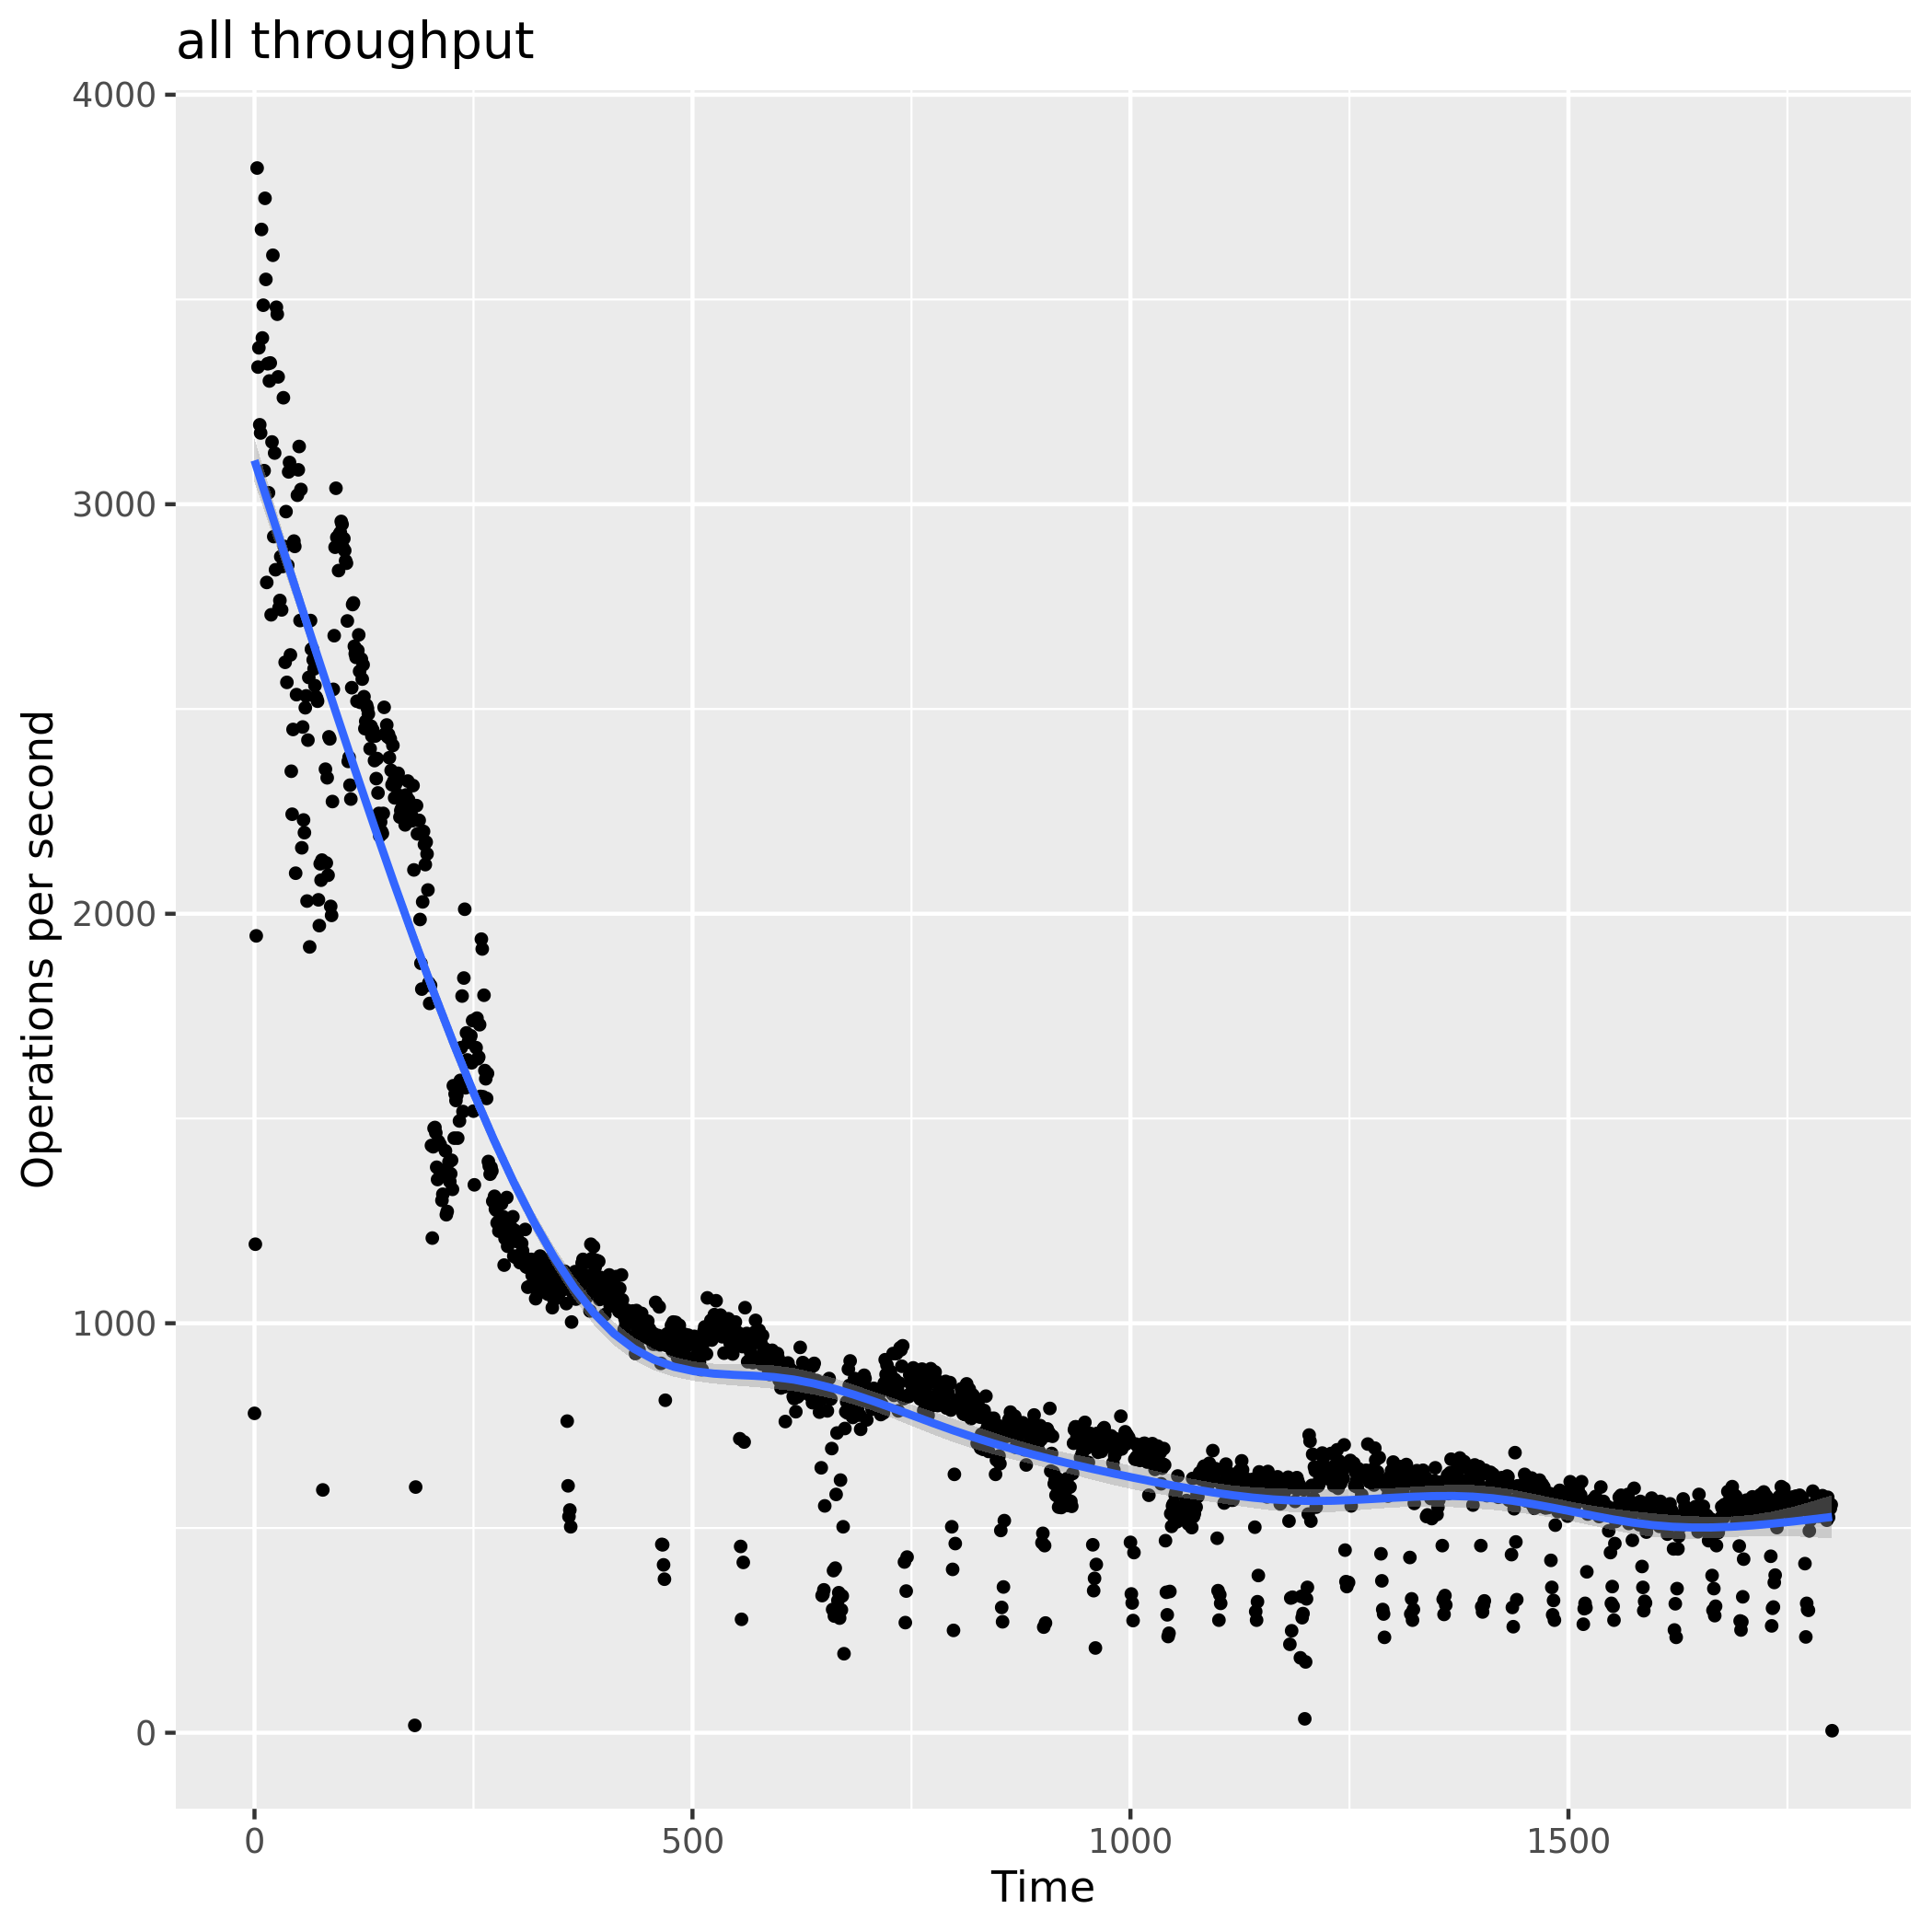
\includegraphics[width=0.5\textwidth]{ConsistentHashing_C1_write_heavy_throughput}
\caption[Throughput Anomaly]{Throughput Anomaly. The throughput shows a steep linear decrease before changing to a shallower linear decrease.}
\label{fig:throughput_anomaly}
\end{figure}

\subsubsection{High Throughput During Handoff}
We expected the benchmark to show a lower throughput and higher latency during the handoffs after a cluster change in the dynamic configuration.
However, as \cref{fig:handoff_anomaly} shows, shortly after the cluster changes at 600s and 1200s the throughput rises to rates much higher than before the change and the latency goes to 0.
This can be explained in one part by rclref vnodes are not handling requests during the handoff and just acknowledging it, and in another part that rclref uses one ets table per vnode and as a consequence of the cluster change there are new vnodes with empty ets tables.
\begin{figure}
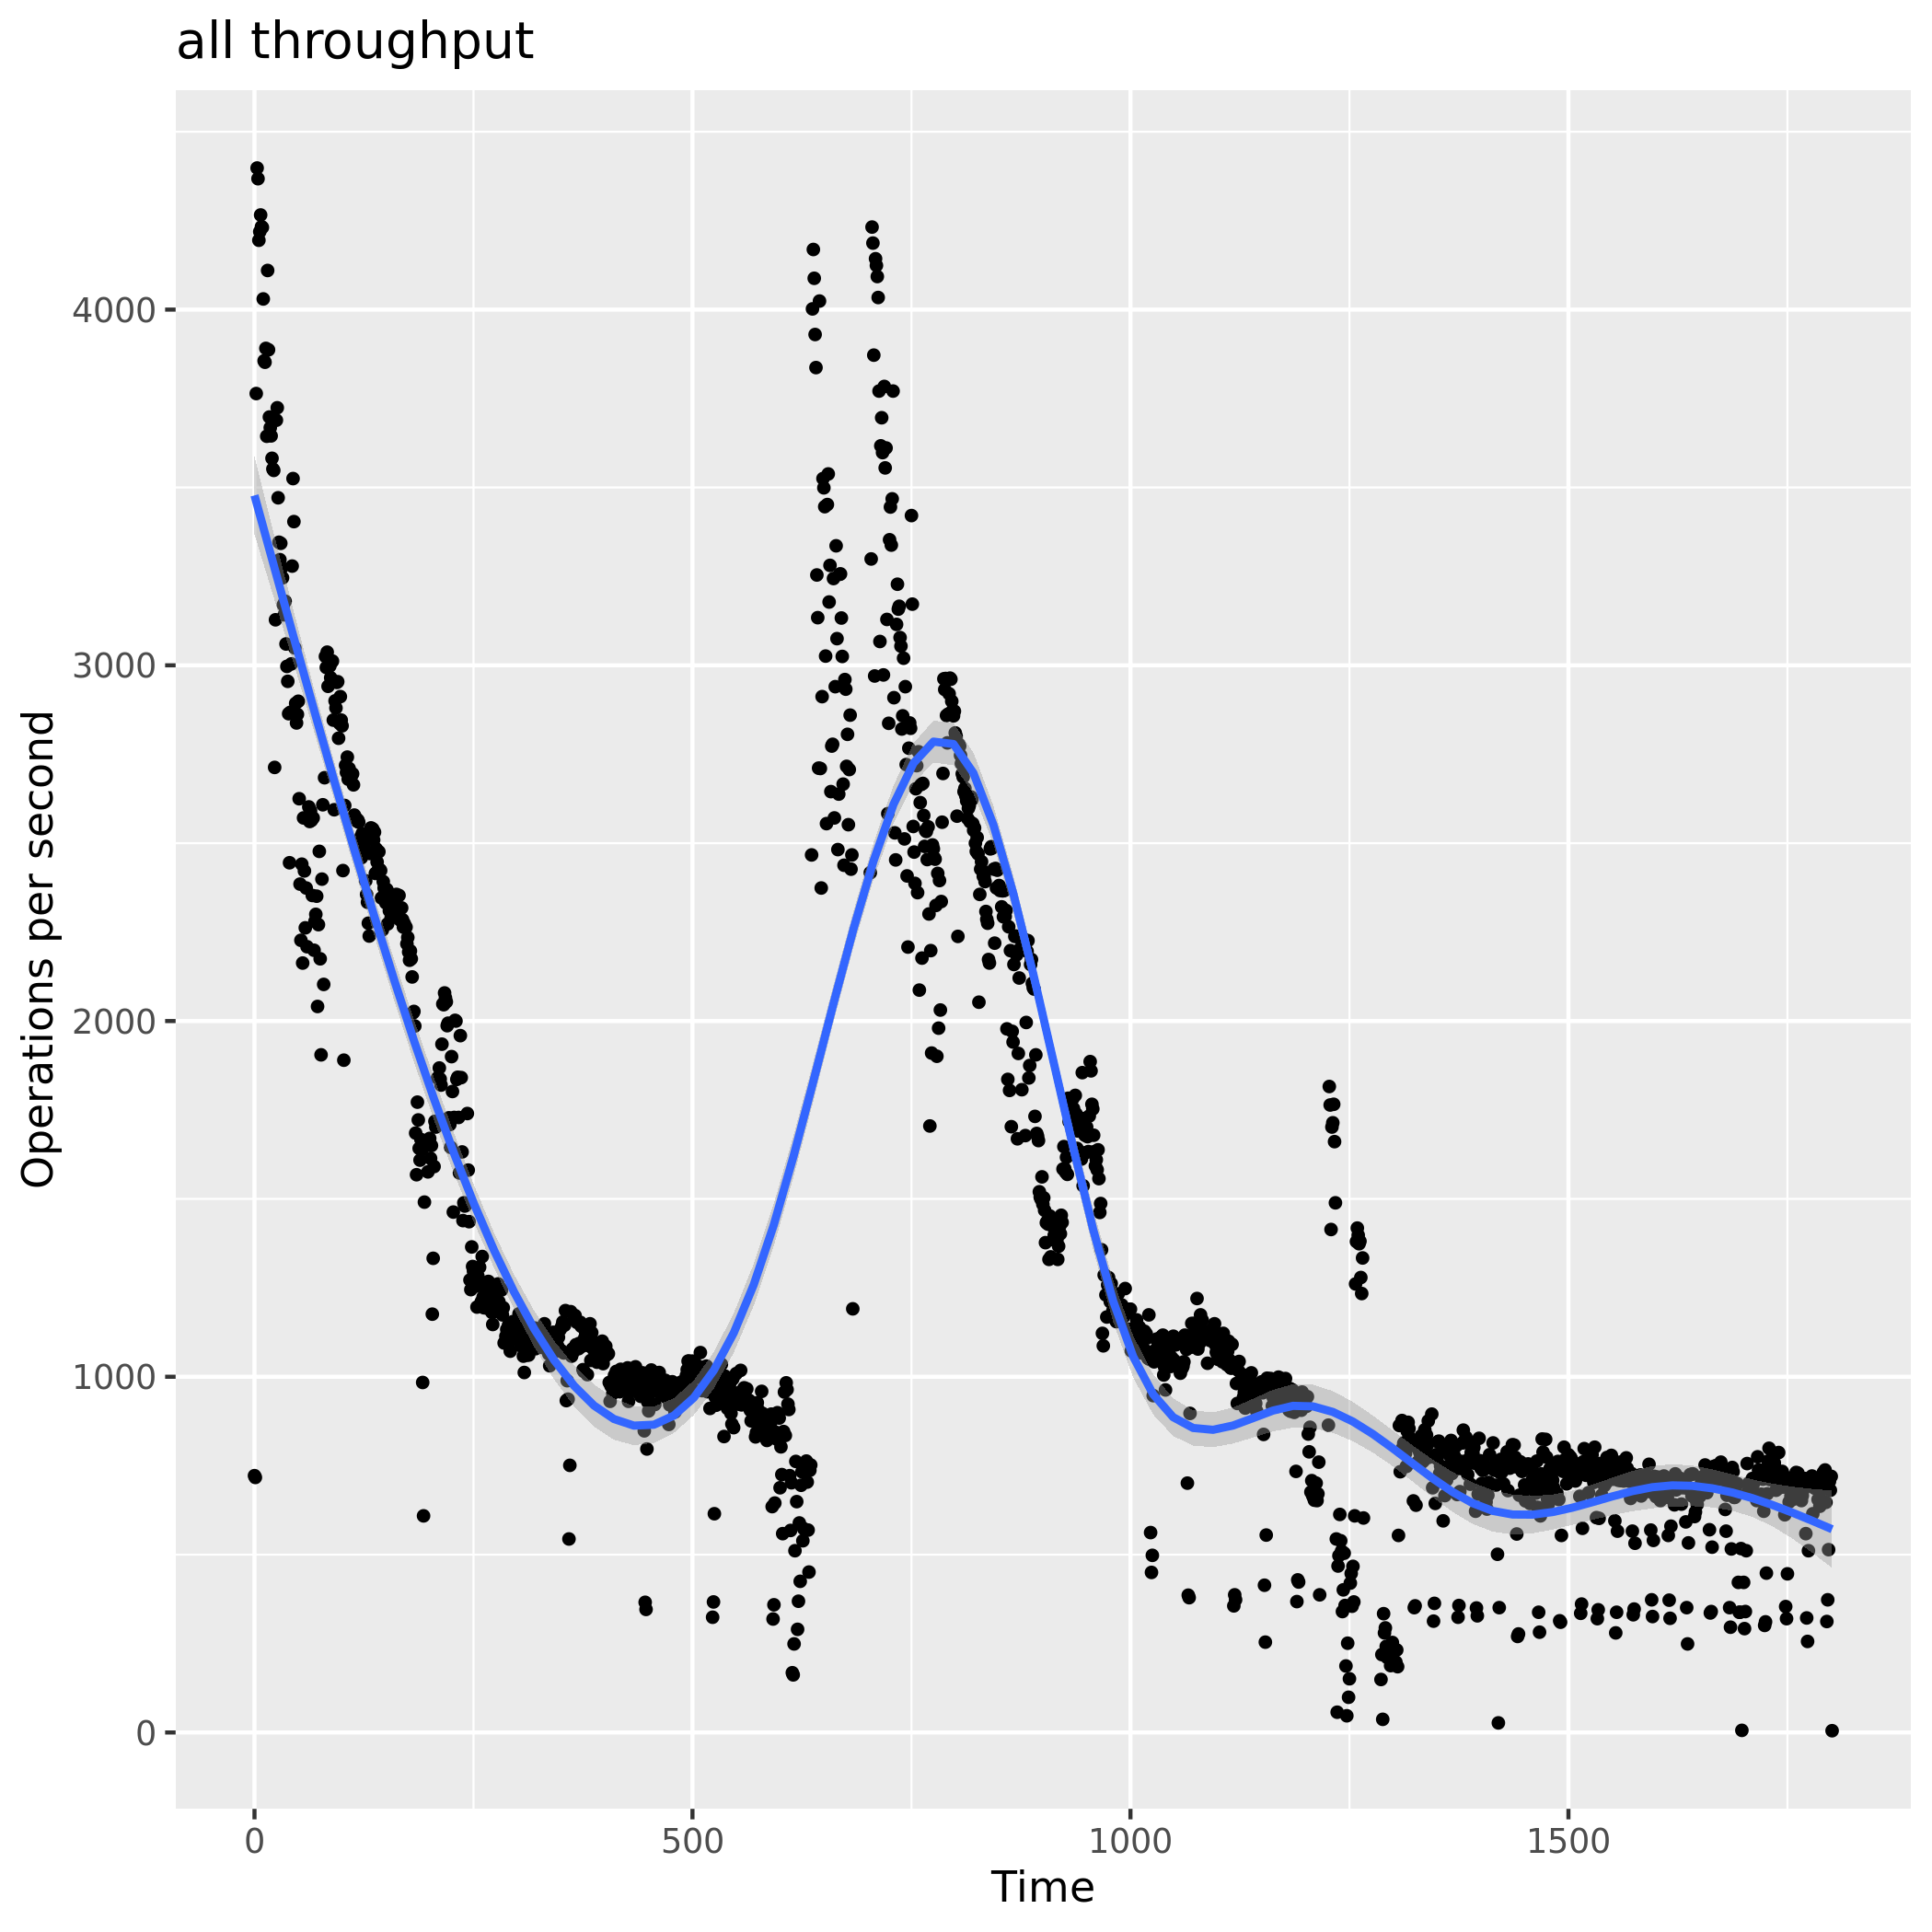
\includegraphics[width=0.5\textwidth]{ConsistentHashing_dynamic_write_heavy_throughput}
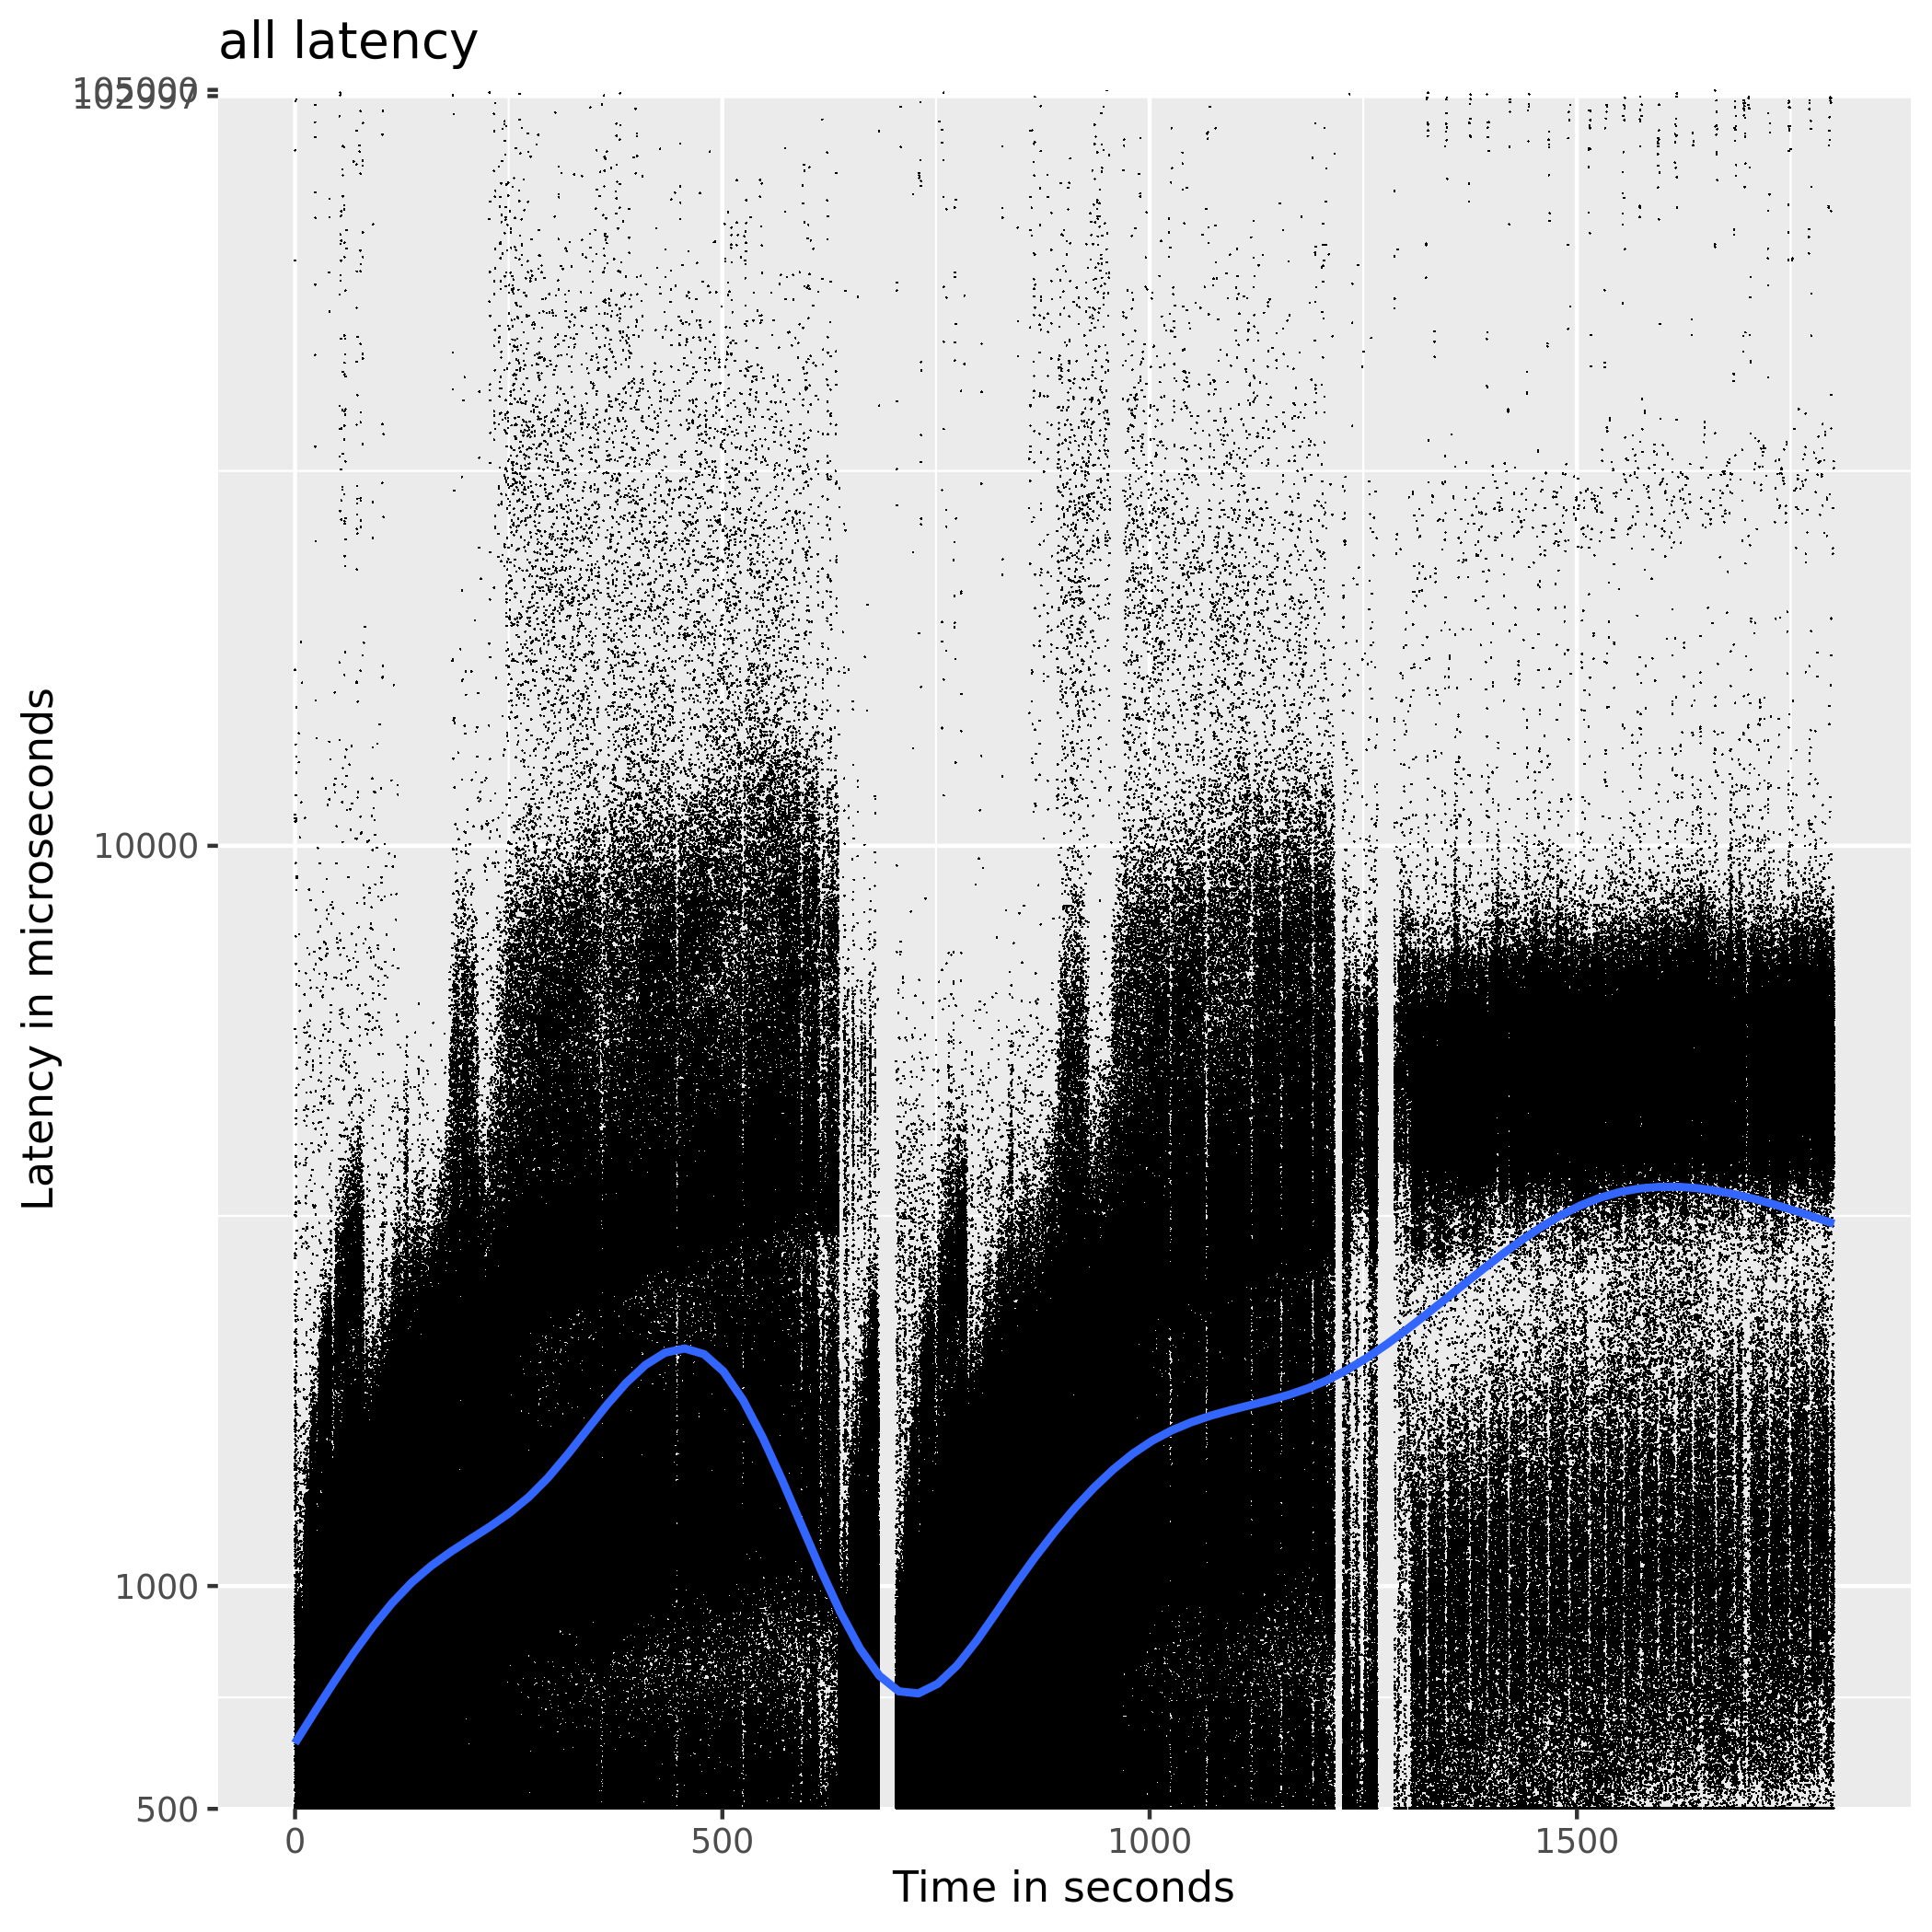
\includegraphics[width=0.5\textwidth]{ConsistentHashing_dynamic_write_heavy_latency}
\caption[Handoff Anomaly]{Handoff Anomaly. Instead of a low throughput and high latency after a cluster change the system has a high throughput and low latency.}
\label{fig:handoff_anomaly}
\end{figure}

\subsubsection{Optimal Load Balance in C0 with Random Slicing}
In configuration C0 with just three nodes \ac{RS} achieves a perfect load balance with the exact same number of keys stored on each node with any of the \acp{RPS}.
This can easily be explained by the nature of \ac{RS}.
Since the three nodes are the initial configuration, \ac{RS} produces a ring with exactly three sections, one for each node.
With $n=3$ set in the configuration each key is therefore replicated on three sections, which leads to each node storing each key and therefore owning the same number of keys.
As for configurations with Consistent Hashing the ring size is set to 64 the sections cannot be perfectly assigned to three nodes and therefore this configuration does not achieve a perfect load balance.

\subsection{Consistent Hashing}
With Consistent Hashing there is no significant difference between read-heavy and write-heavy workloads.
A visualization of runs in C0 and C2 is shown in \cref{fig:throughput_consistent_hashing}
There is a clear trend of lower throughput with a higher number of nodes.
In configuration C0 with three nodes the average throughput starts at about 3500 operations per second, steeply decreases to 1000 operations per second at about 450s and from there slowly decreases to 500 operations per second.
In configuration C1 with four nodes there is no clear difference to C0.
However, in configuration C2 with seven nodes the average throughput starts at about 750 operations per second, there is no steep decrease, and it slowly decreases to 450 operations per second.
One can see, that while starting out at a way lower rate the throughput ends up at a closer rate between the configurations.
\begin{figure}
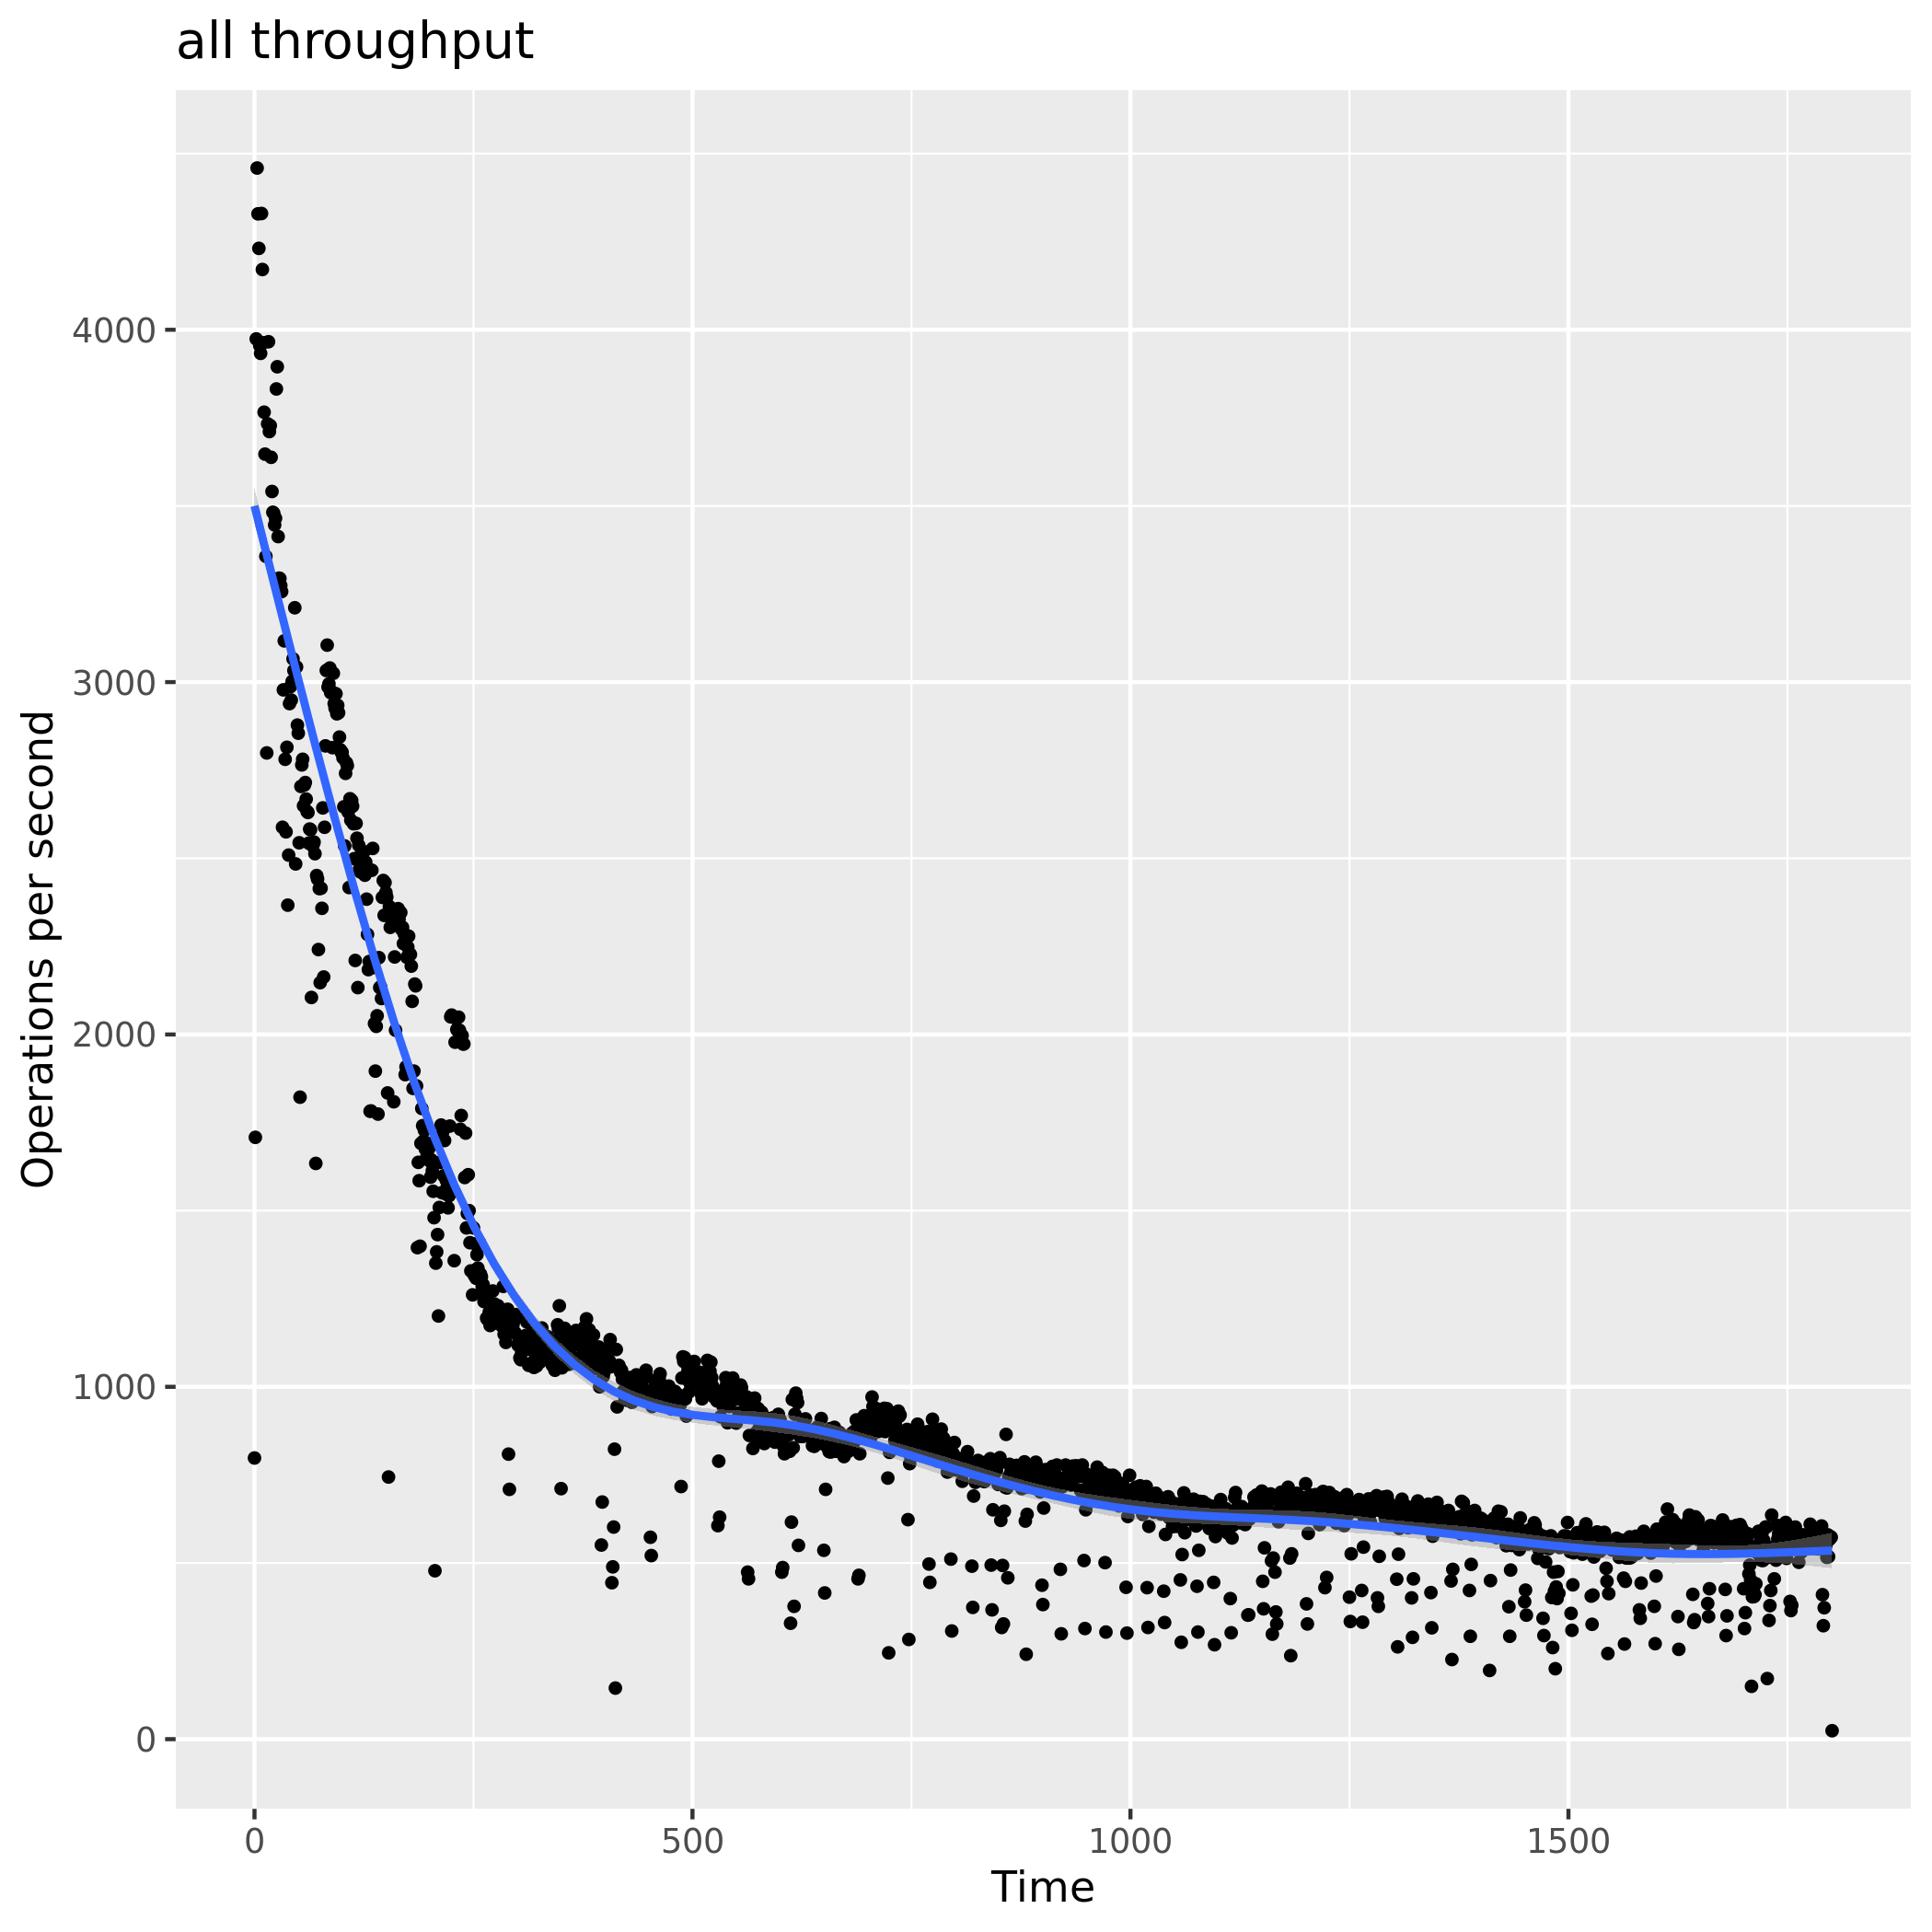
\includegraphics[width=0.5\textwidth]{ConsistentHashing_C0_write_heavy_throughput}
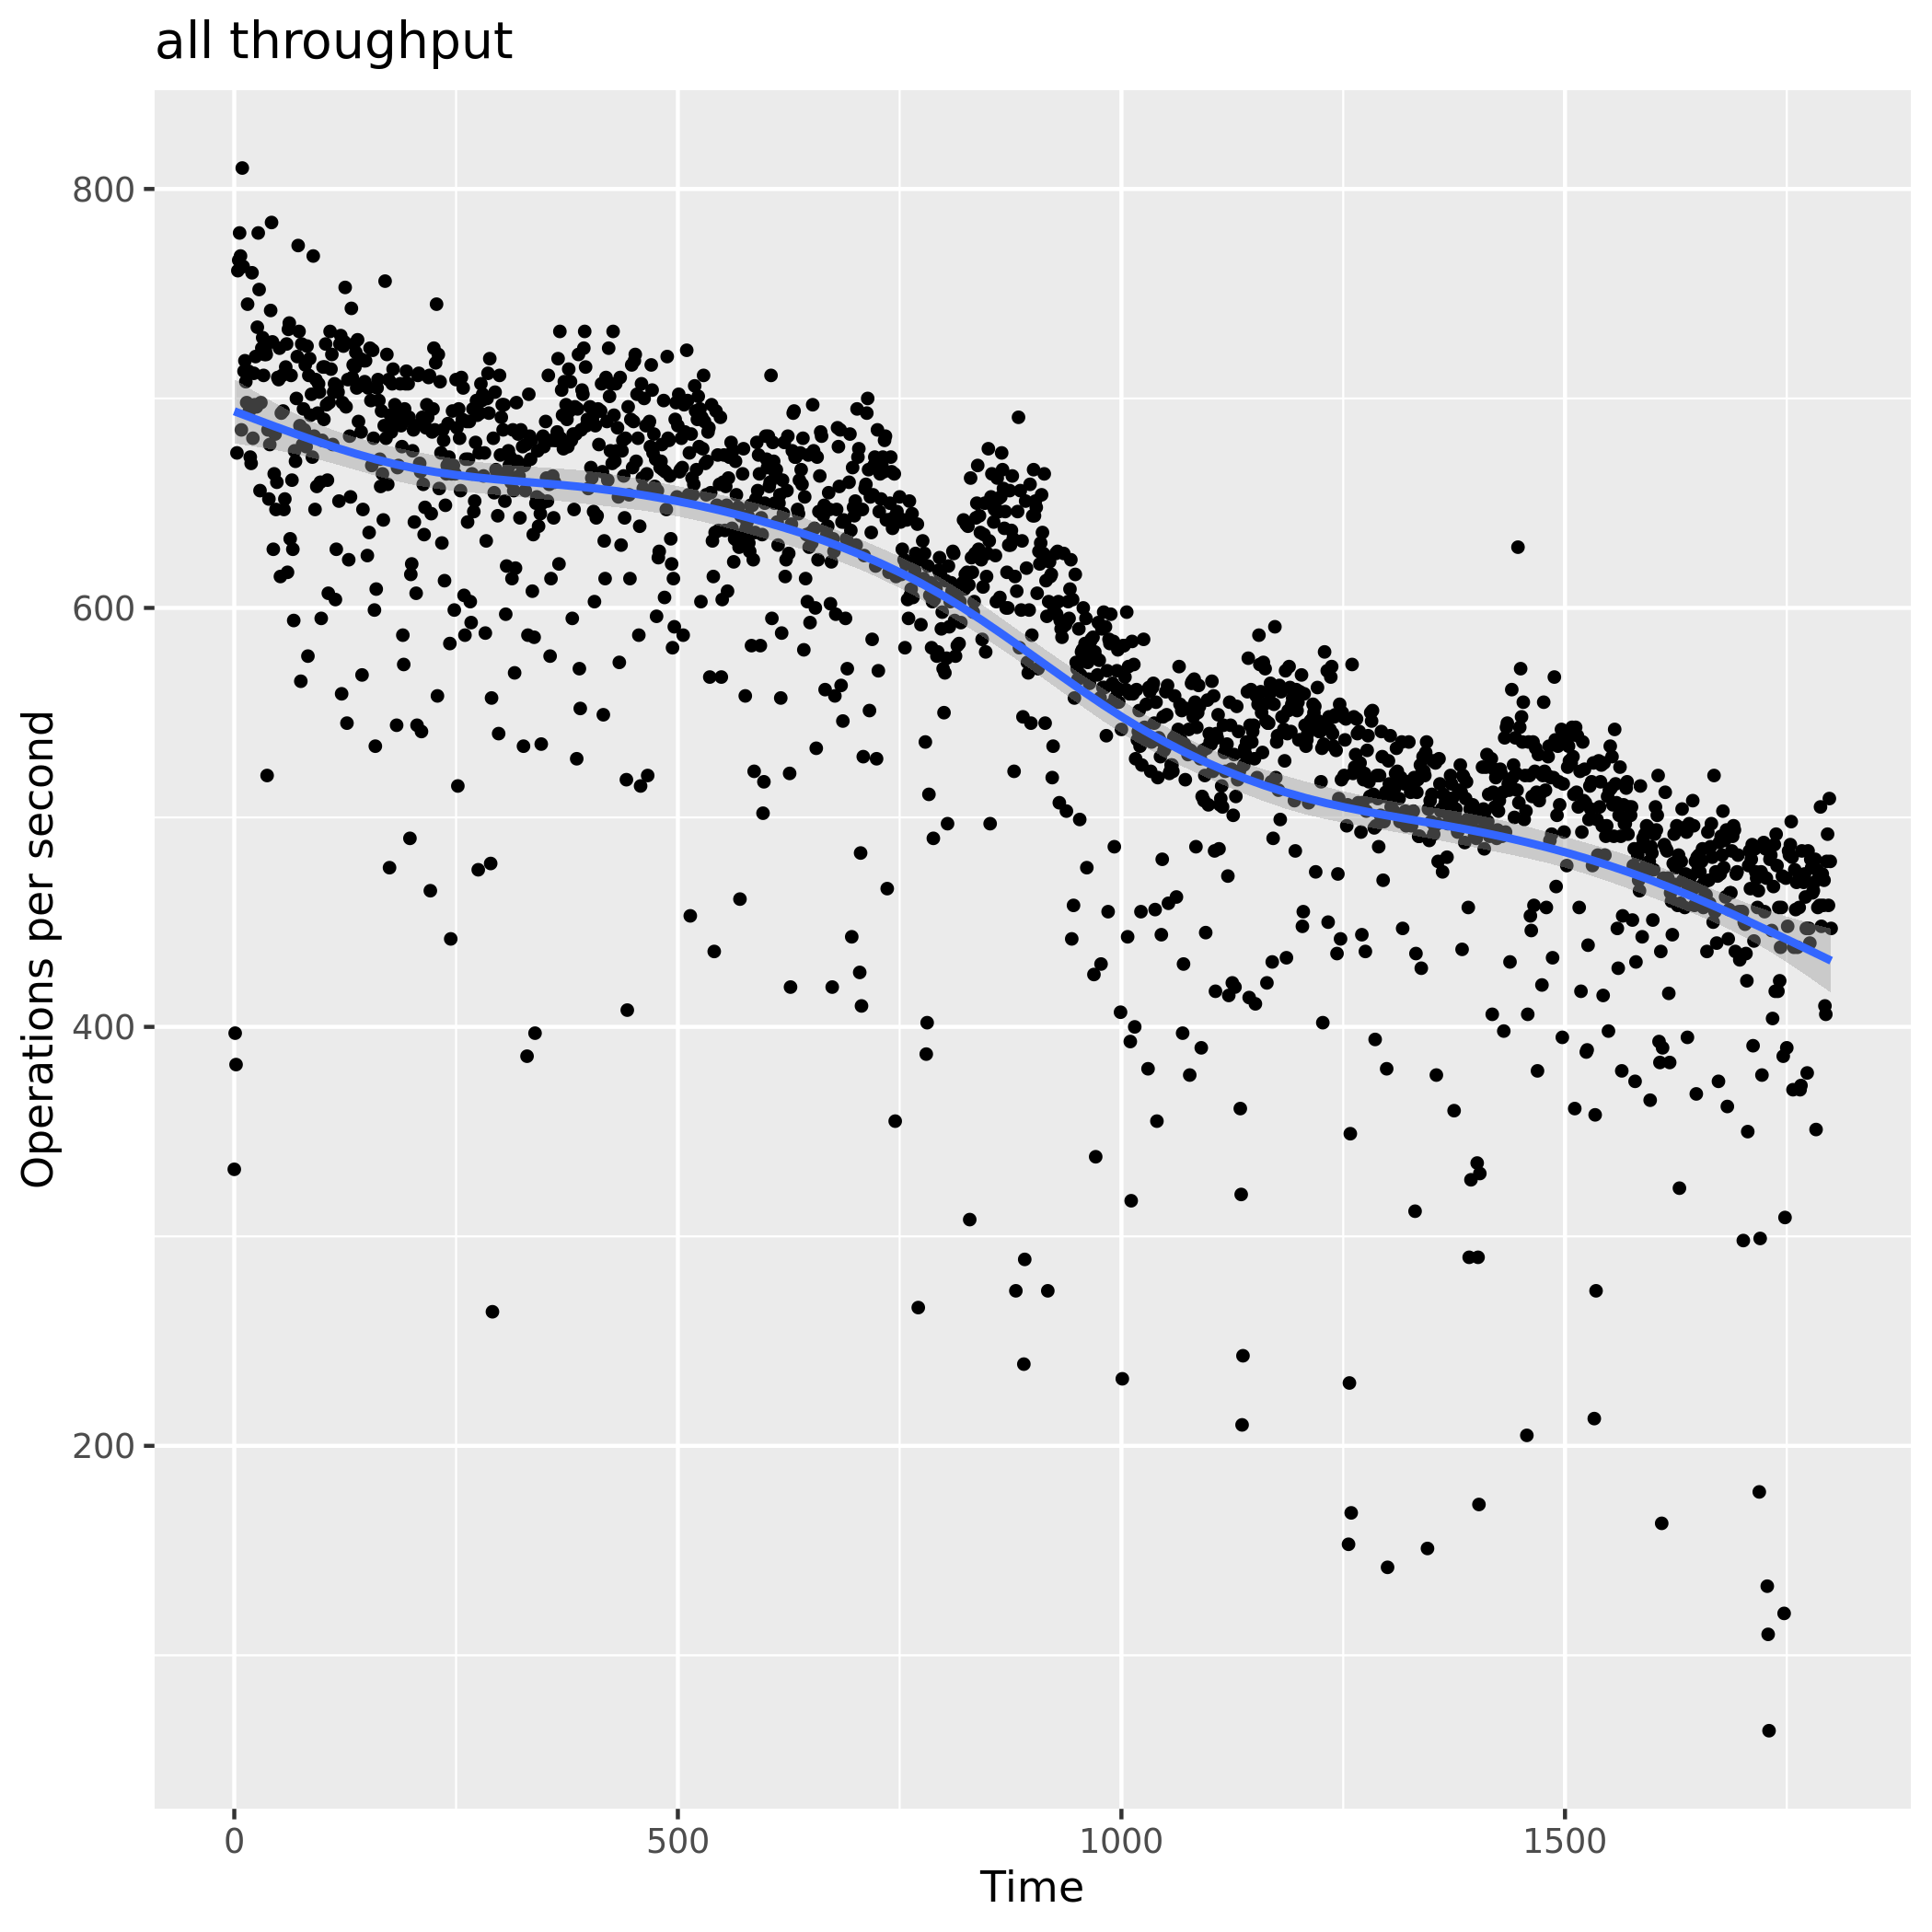
\includegraphics[width=0.5\textwidth]{ConsistentHashing_C2_write_heavy_throughput}
\caption[Consistent Hashing Throughput Comparison]{Consistent Hashing Throughput Comparison. Showing the throughput for Consistent Hashing in C0 and C2 with write-heavy workload.}
\label{fig:throughput_consistent_hashing}
\end{figure}

For the dynamic benchmark runs there are significant differences between read-heavy and write-heavy workload.
Ignoring the impact of the cluster changes the throughput plot seems to be quite similar as it decreases to 1000 operations per second within 450 seconds and after that decreases to about 600 operations per second.
However, it seems that for the read-heavy workload the change from C0 to C1 does not have a great impact on the throughput or latency while it has a significant impact during the write-heavy workload.
This can be seen both in the throughput and latency plots in \cref{fig:consistent_hashing_dynamic}.
For the change from C1 to C2 at 1200s the impact of the workload seems to be inverse to the ones of the change from C0 to C1.
\begin{figure}
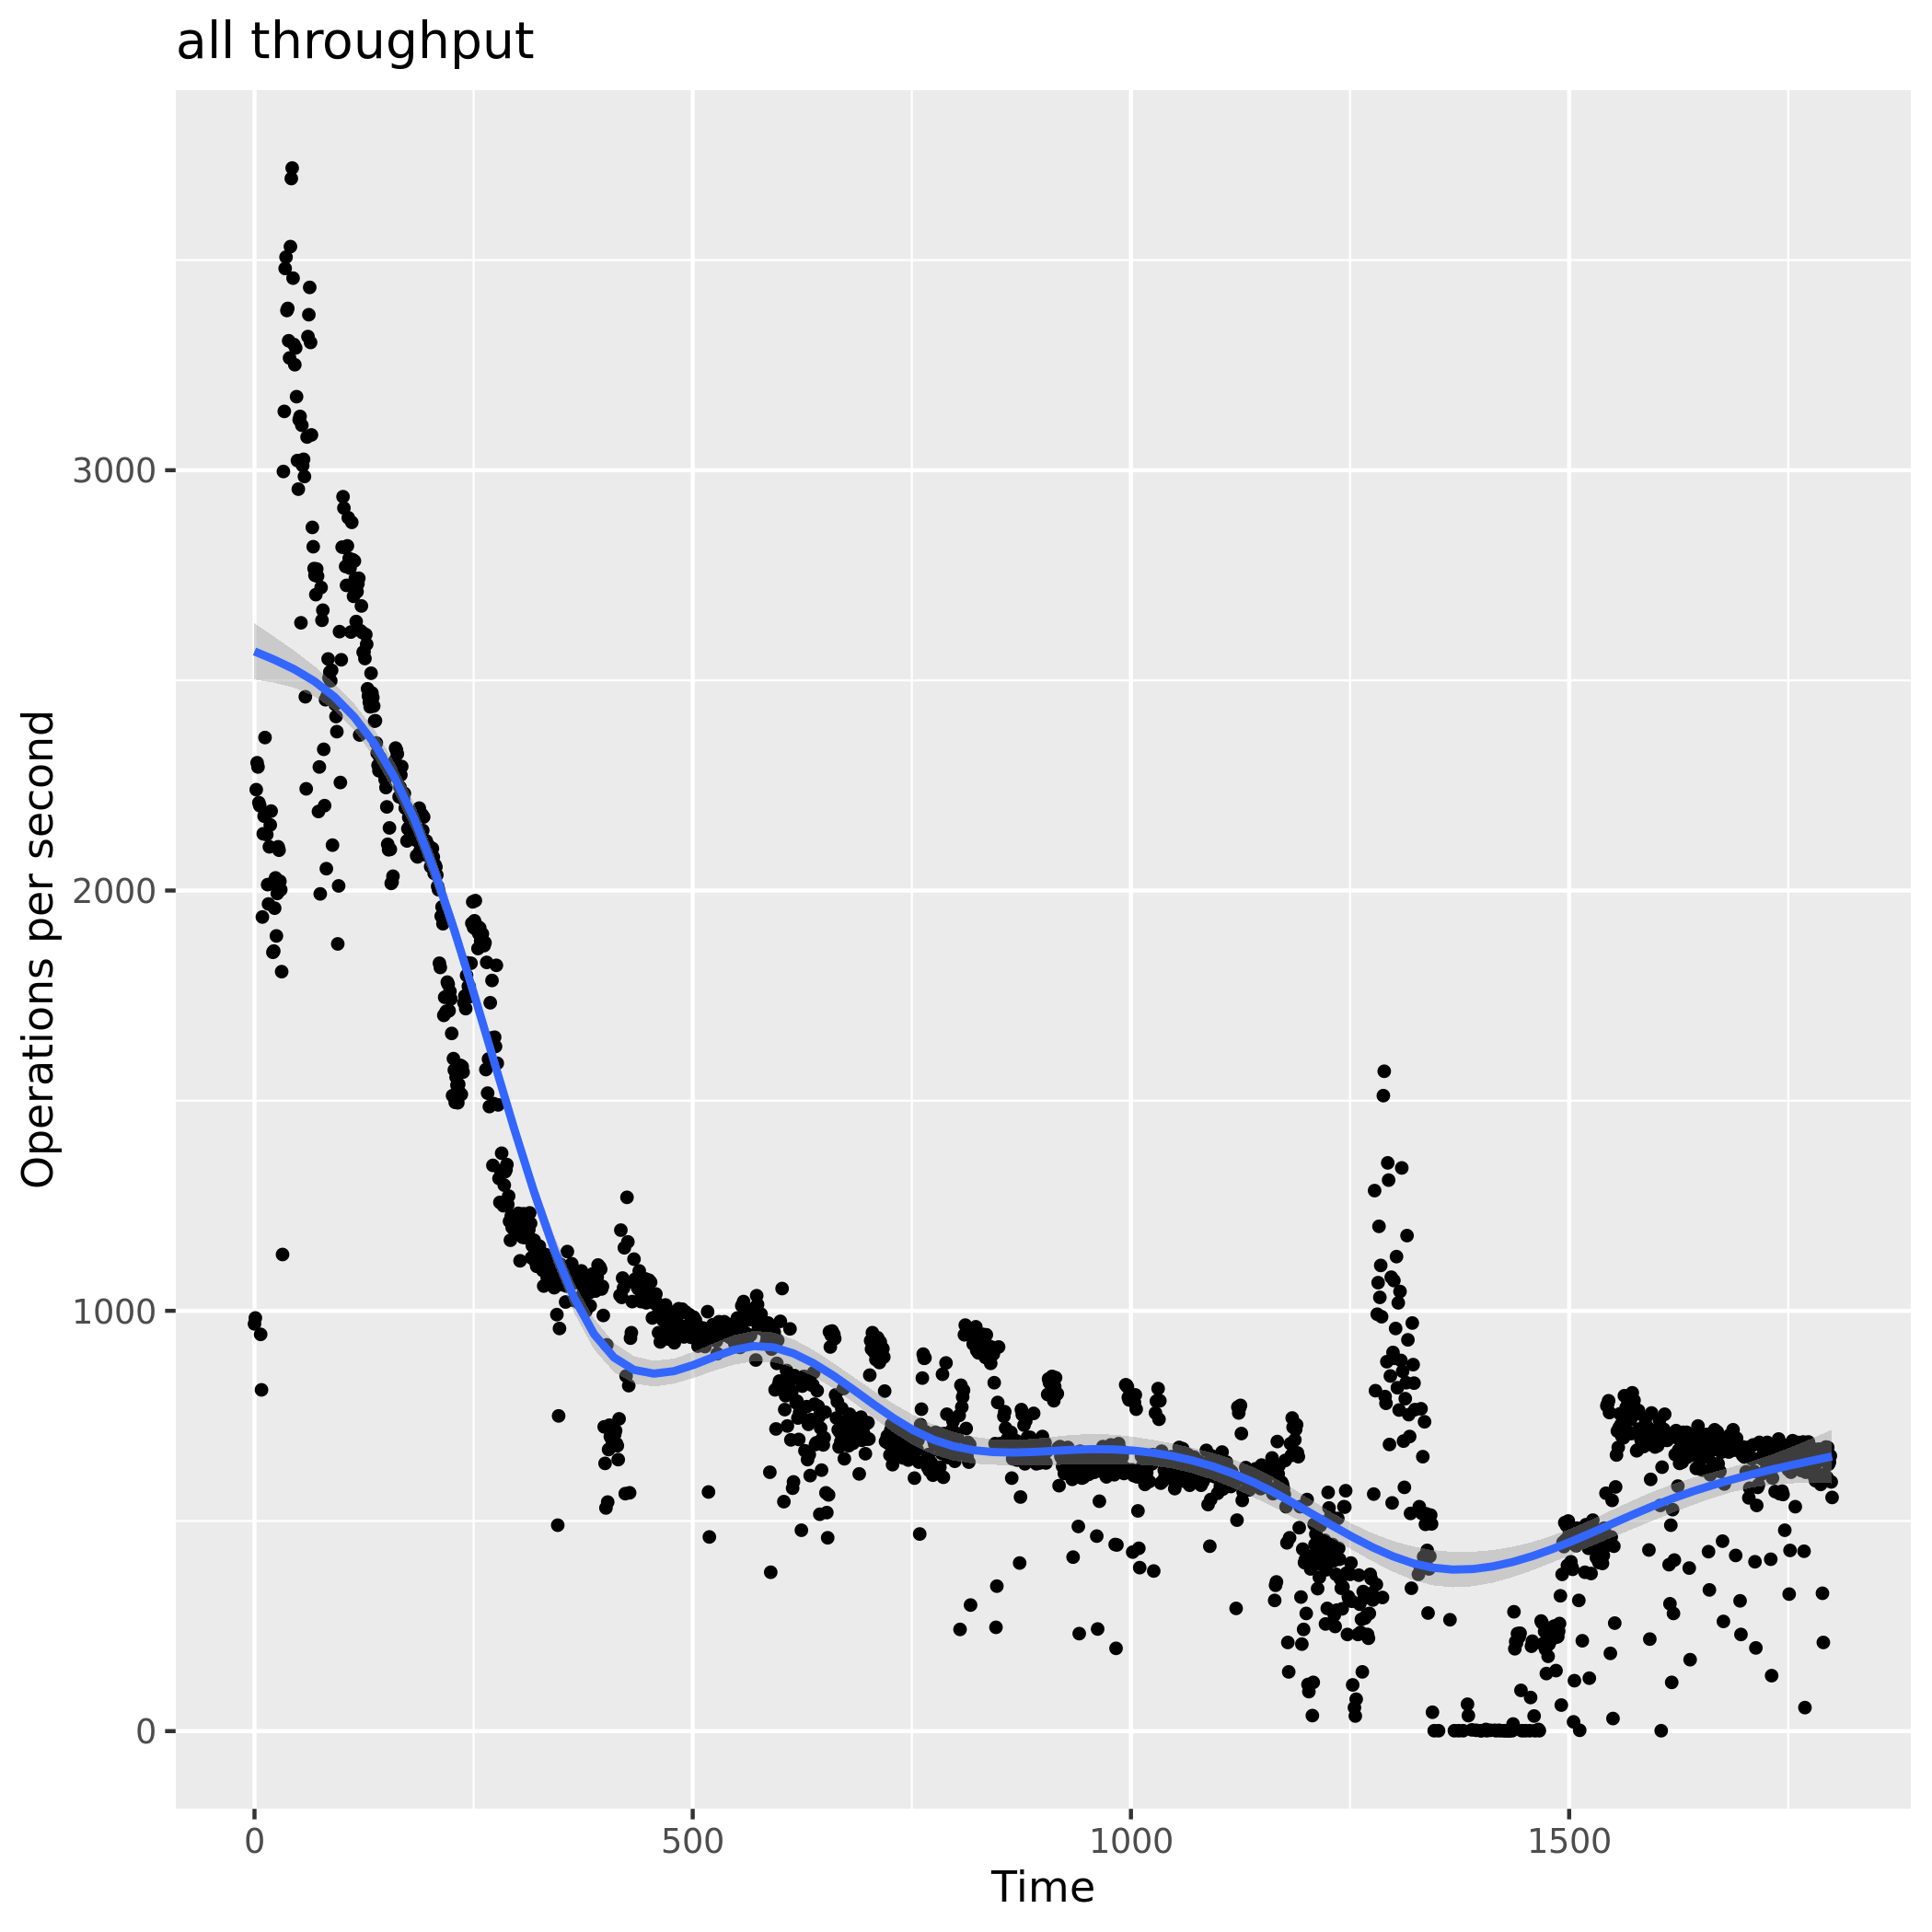
\includegraphics[width=0.5\textwidth]{ConsistentHashing_dynamic_read_heavy_throughput}
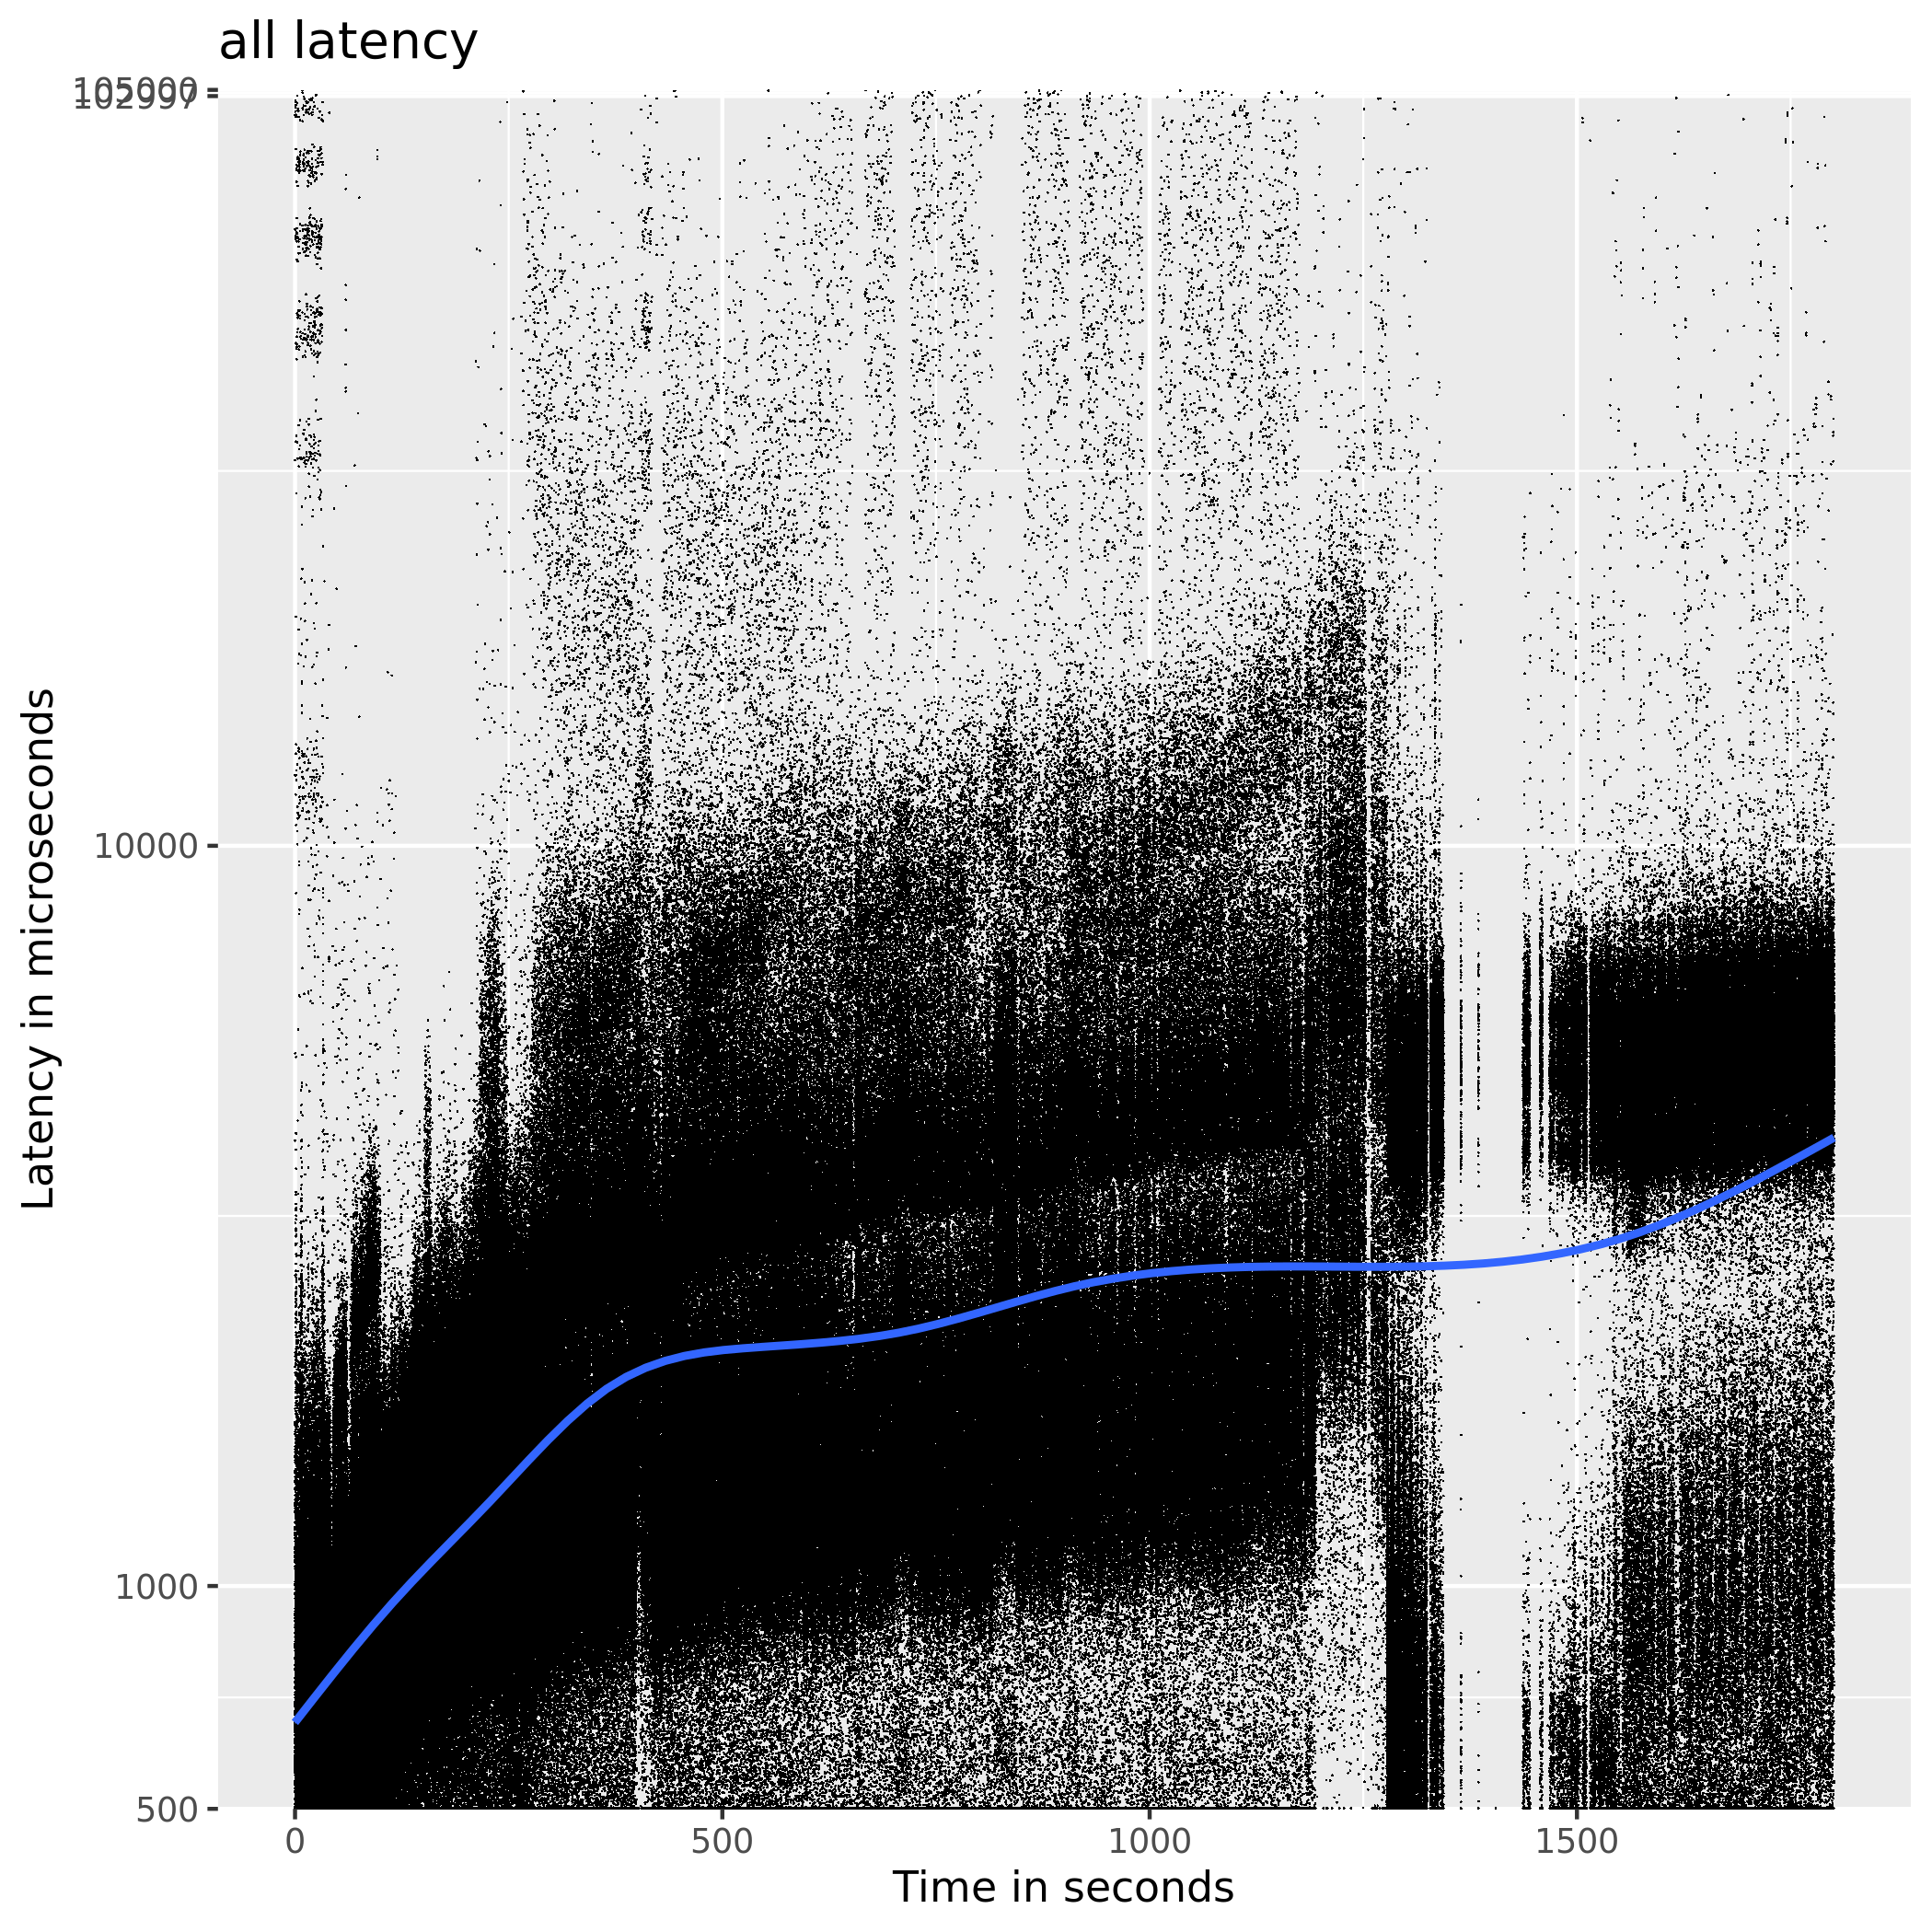
\includegraphics[width=0.5\textwidth]{ConsistentHashing_dynamic_read_heavy_latency}
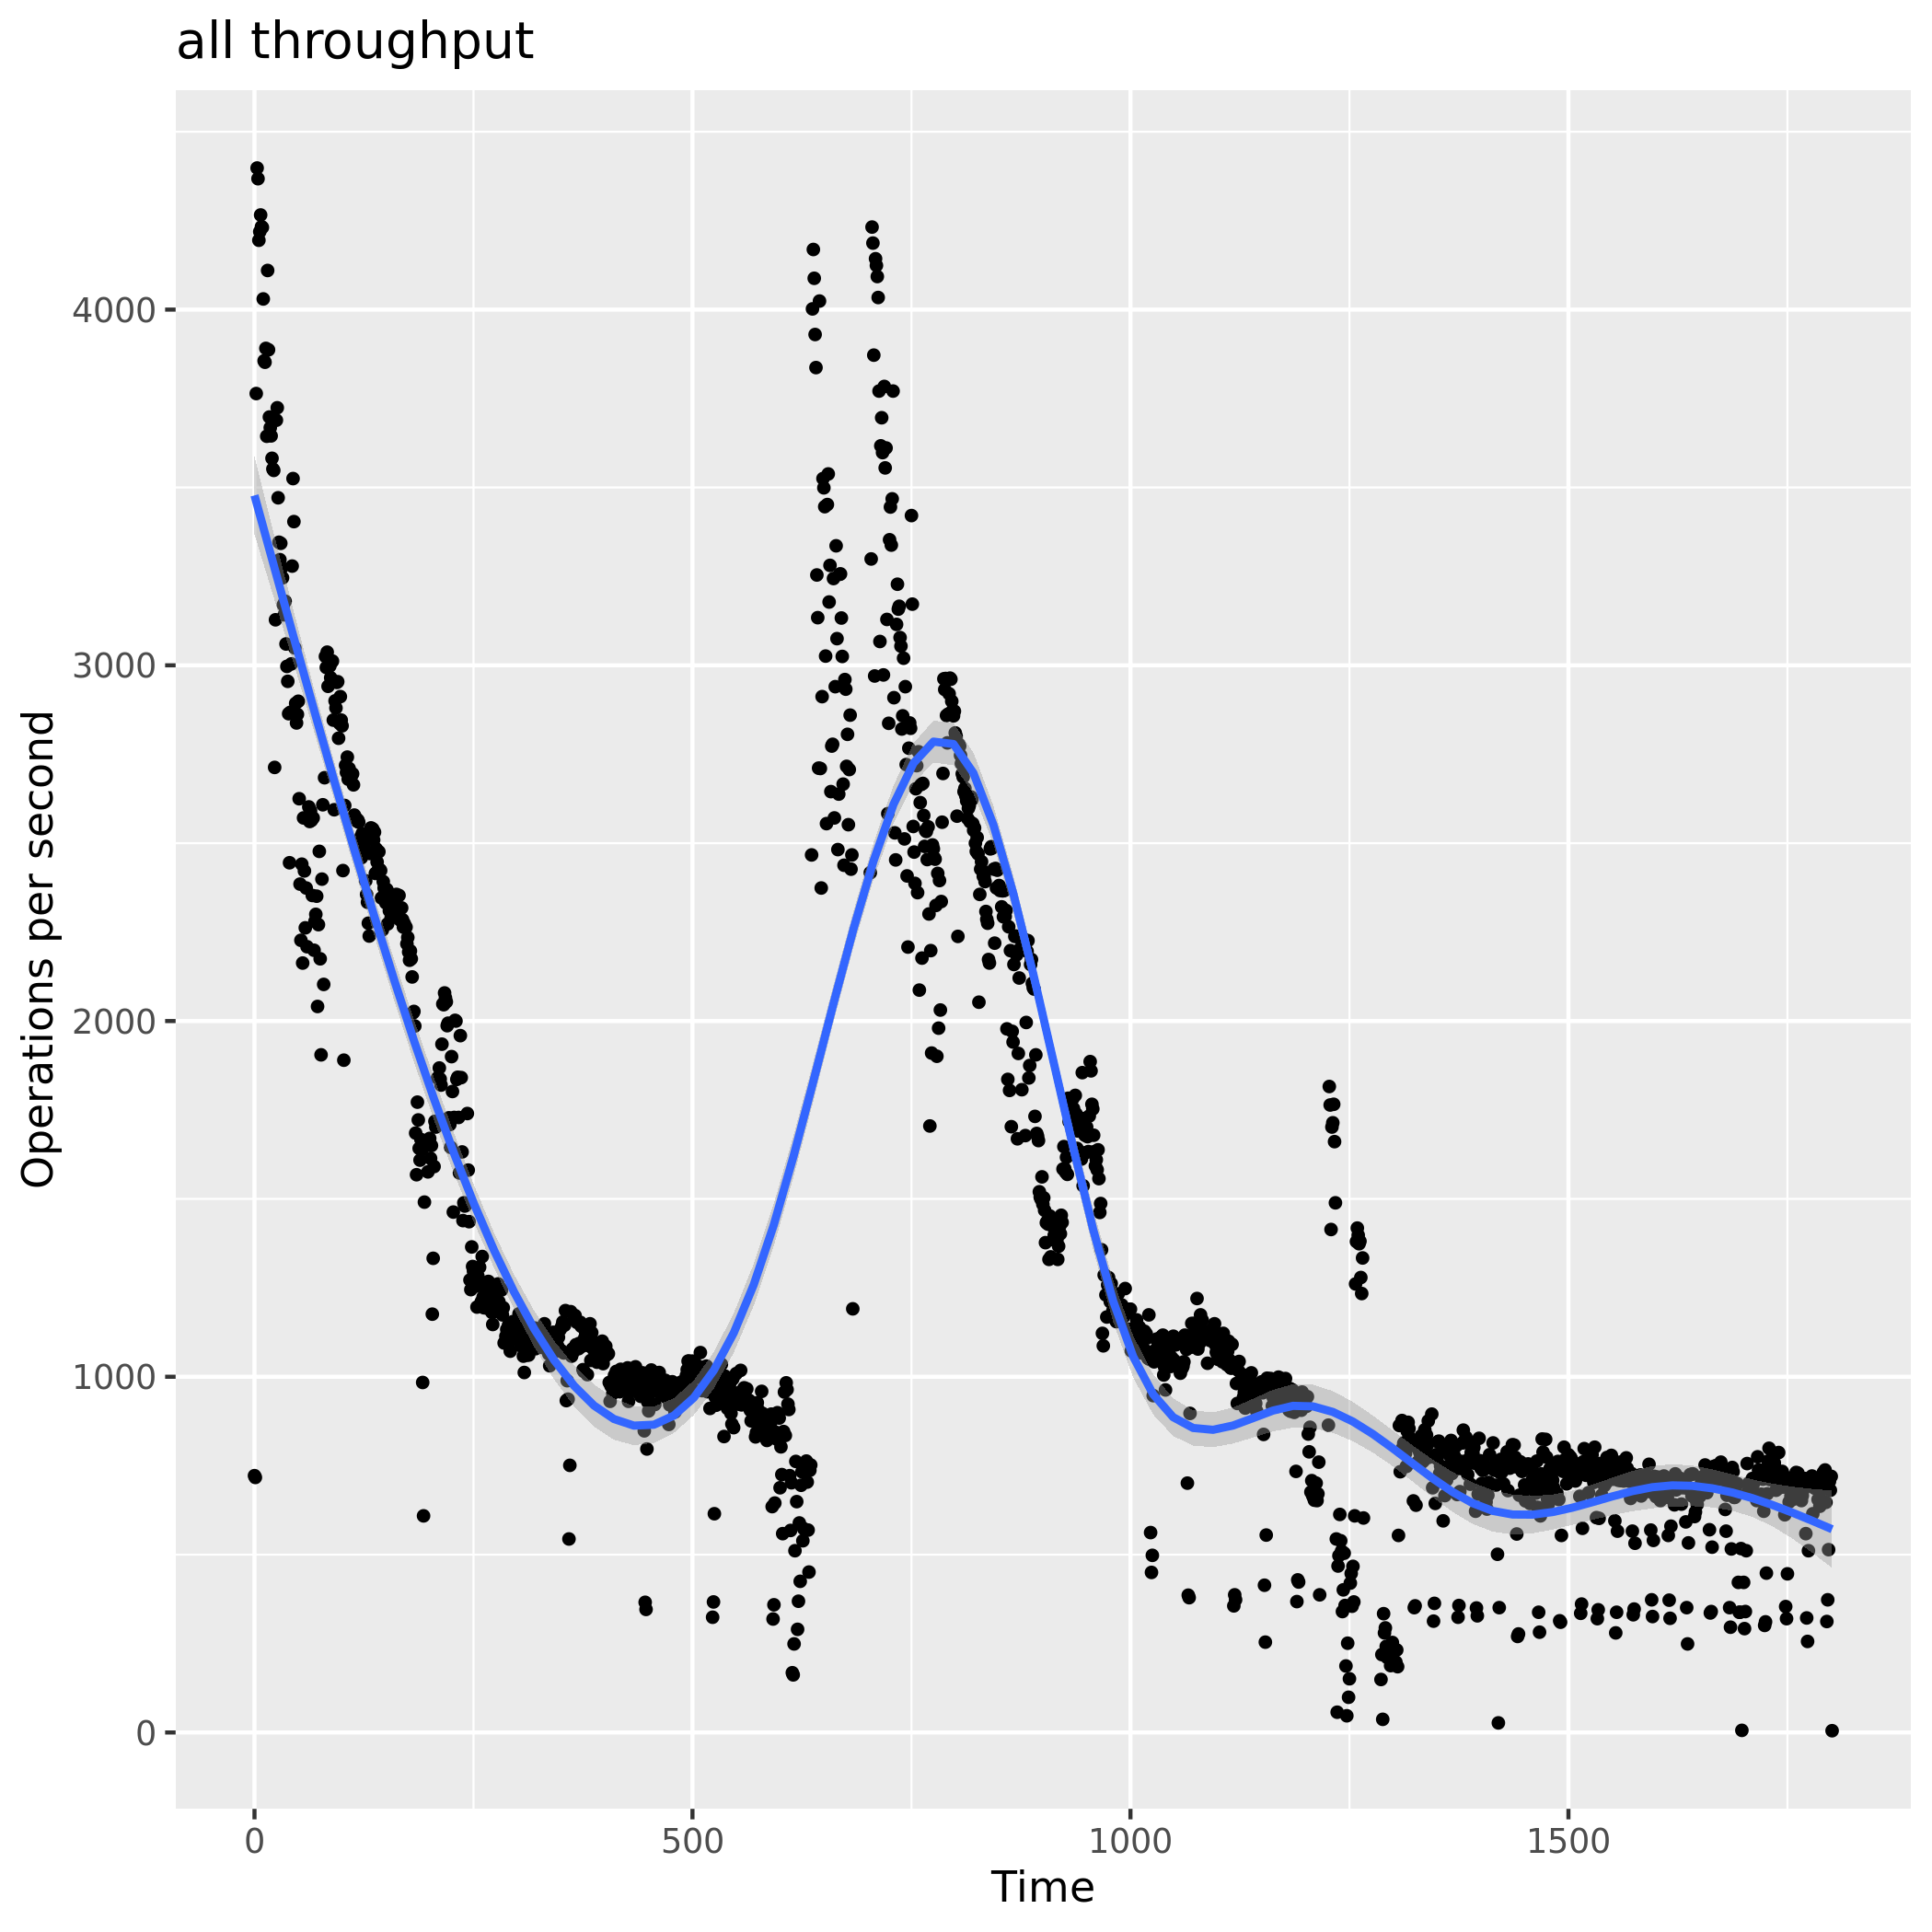
\includegraphics[width=0.5\textwidth]{ConsistentHashing_dynamic_write_heavy_throughput}
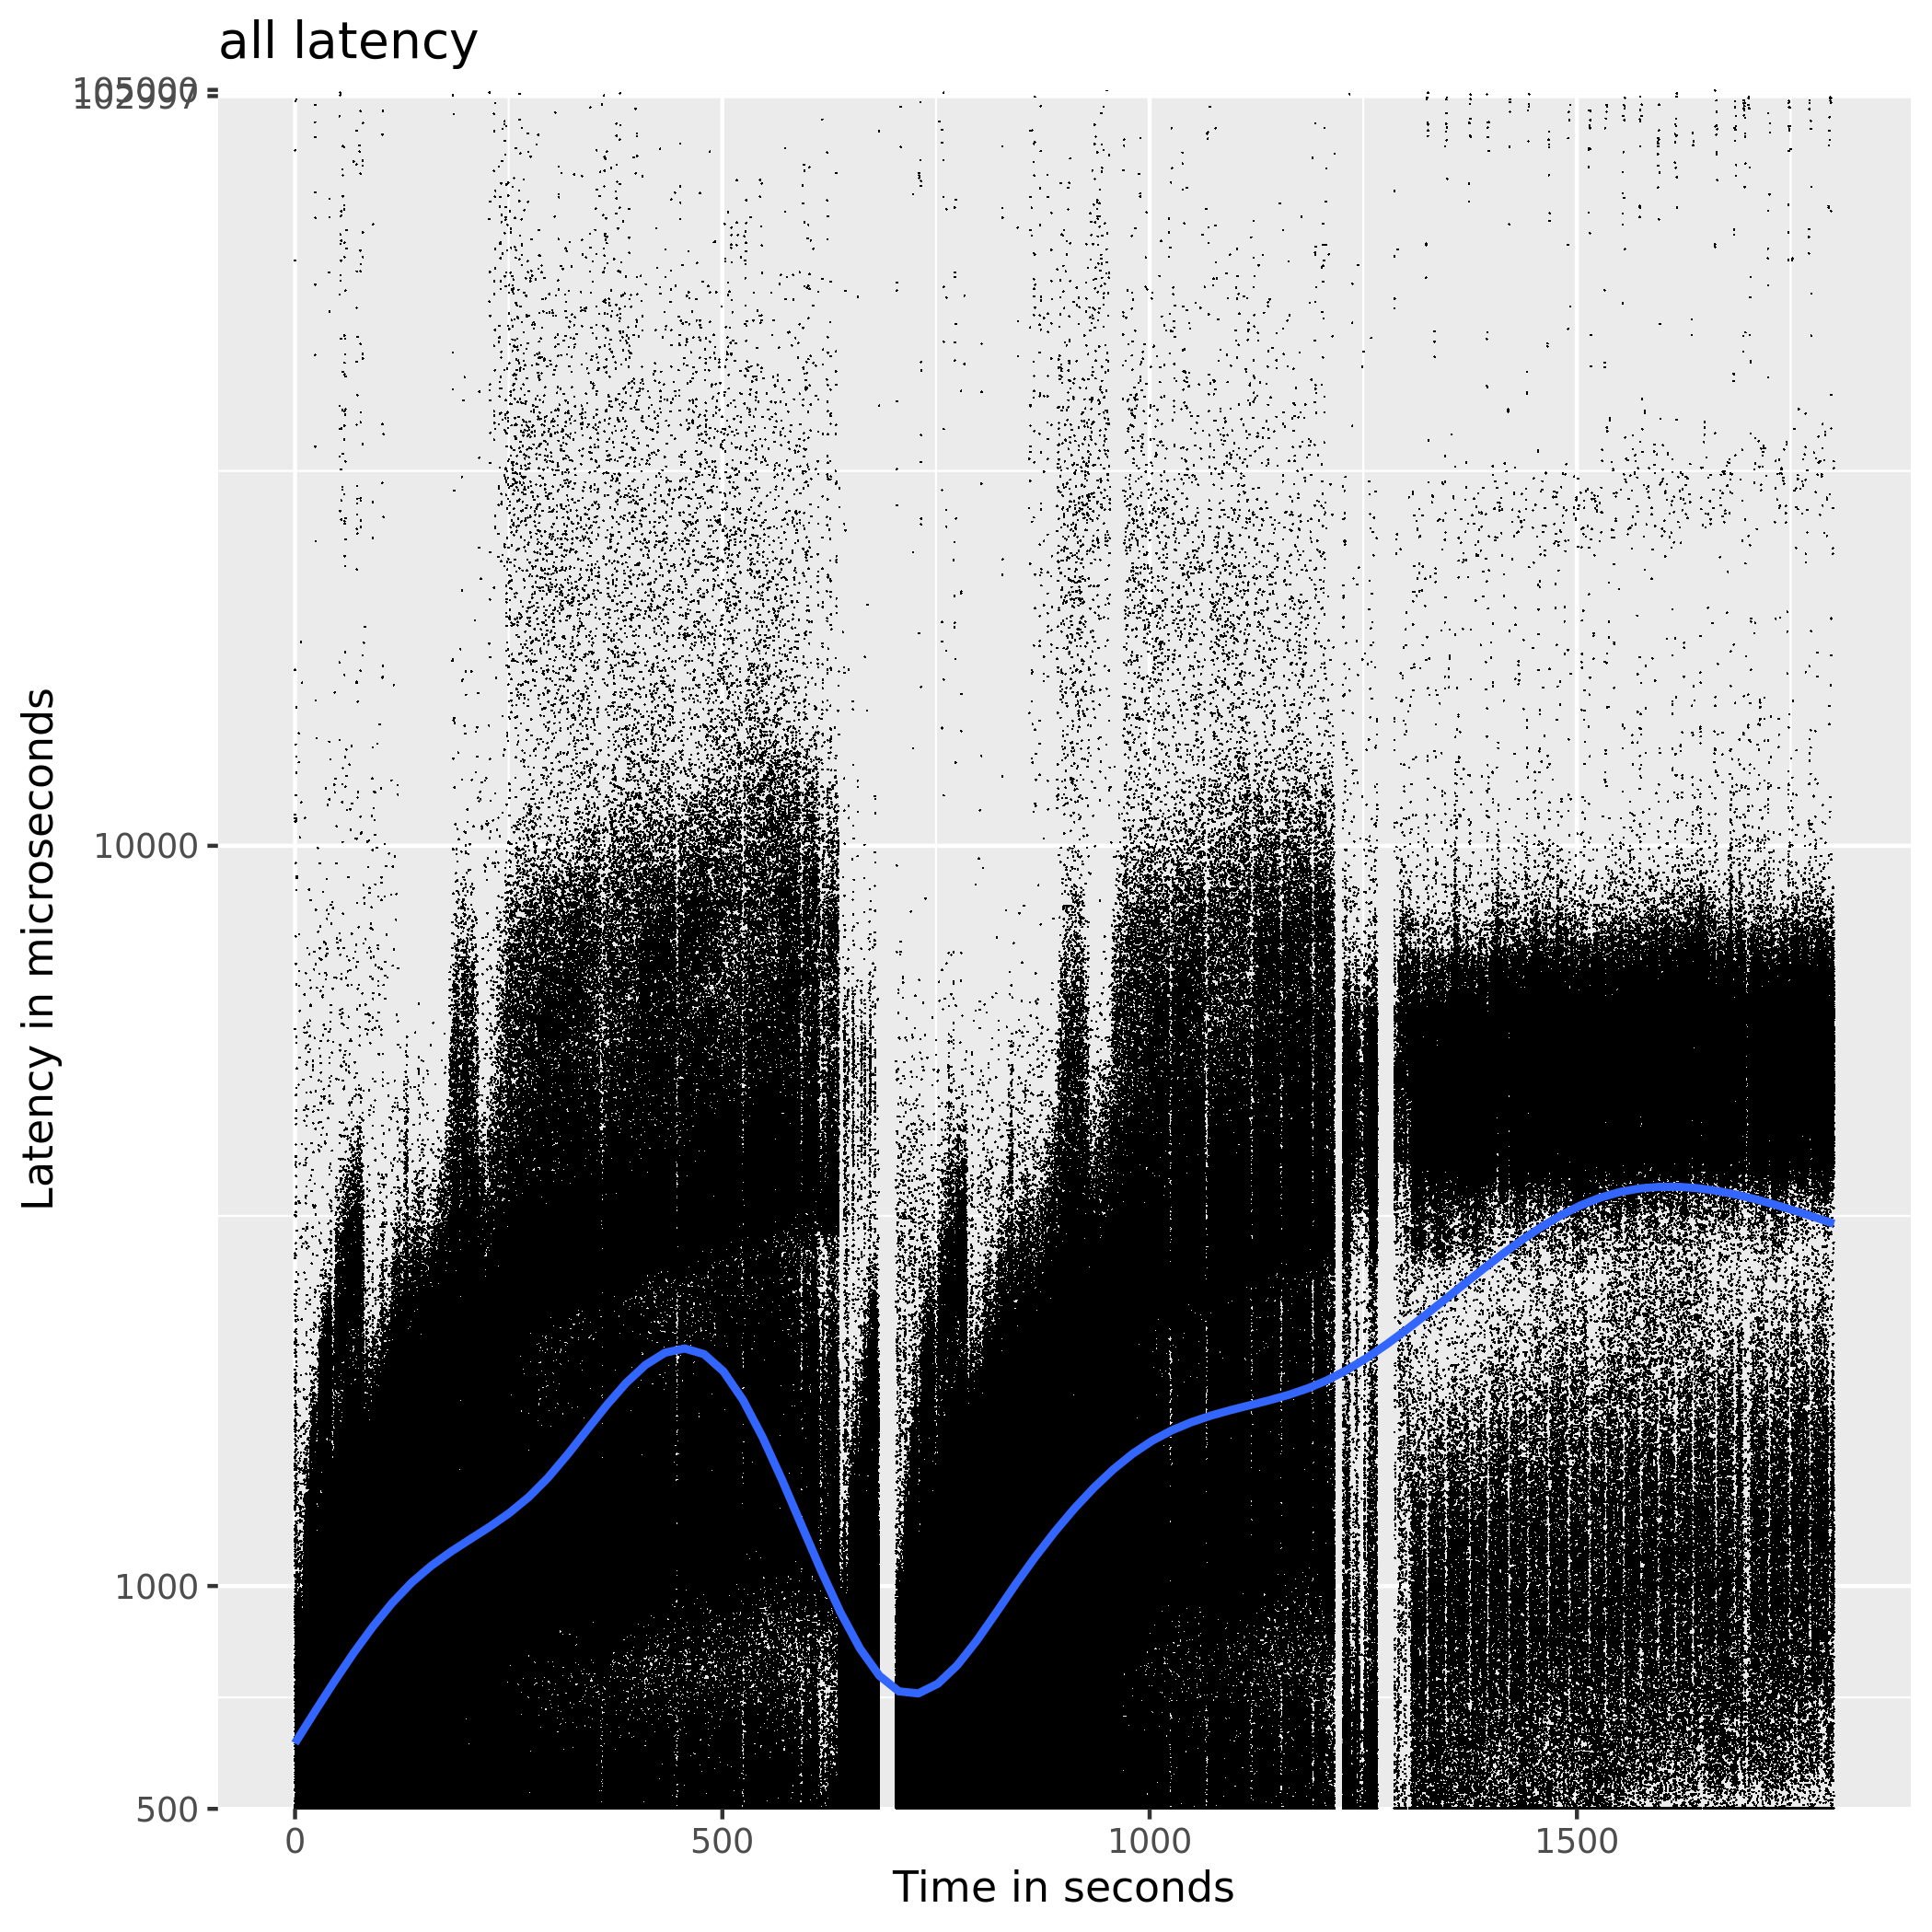
\includegraphics[width=0.5\textwidth]{ConsistentHashing_dynamic_write_heavy_latency}
\caption[Dynamic Runs with Consistent Hashing]{Dynamic Runs with Consistent Hashing. There is a difference how cluster changes influence throughput and latency for read-heavy (top) and write-heavy (bottom) workloads.}
\label{fig:consistent_hashing_dynamic}
\end{figure}
Ignoring the read-heavy dynamic run as an inexplicable anomaly looking at the latency plot for the write-heavy dynamic run seems to show a short impact at 600s and 1200s each that is followed by a longer disruption after a short delay.
Both the phase of initial disruption and the following disruption seem to be longer for the change from C1 to C2.
The initial disruption may be caused by the reconfiguration of the ring and nodes being set to forwarding while the following longer disruption can be explained by the actual handoff operation and potential repair operations.

Regarding the divergence from optimal load balance with Consistent hashing there is an absolute overall average divergence for key load of 0.003821643008703, for put load of 0.032386205130647, and for get load of 0.032384489514972.
The highest divergence is measured with seven nodes in C2 and the lowest in C1 with four nodes.
This is quite intuitive as with four nodes the nodes can be perfectly assigned to the 64 sections of the ring, while with three and seven nodes some nodes have one section more assigned to them than others. 

\subsection{Random Slicing Jumping}
As with Consistent Hashing one cannot see a significant difference between read-heavy and write heavy workloads when looking at the throughput of the system.
A visualization of a run in C0 and C2 is shown in \cref{fig:throughput_random_jumping}.
One can see an influence of the number of nodes in the system on the performance.
This can easily be explained by the higher number of sections and therefore higher lookup time.
In configuration C0 with three nodes the average throughput starts at about 3500 operations per second, steeply decreases to 1000 operations per second at about 450s and from there slowly decreases to 500 operations per second.
The change to four nodes does not significantly change the throughput plot as there are only three new sections on the ring.
However, in configuration C1 with seven nodes the average throughput starts at 1300 and 900 operations per seconds for the read-heavy and write-heavy workload respectively and then decreases for both cases to 500 operations per second.
\begin{figure}
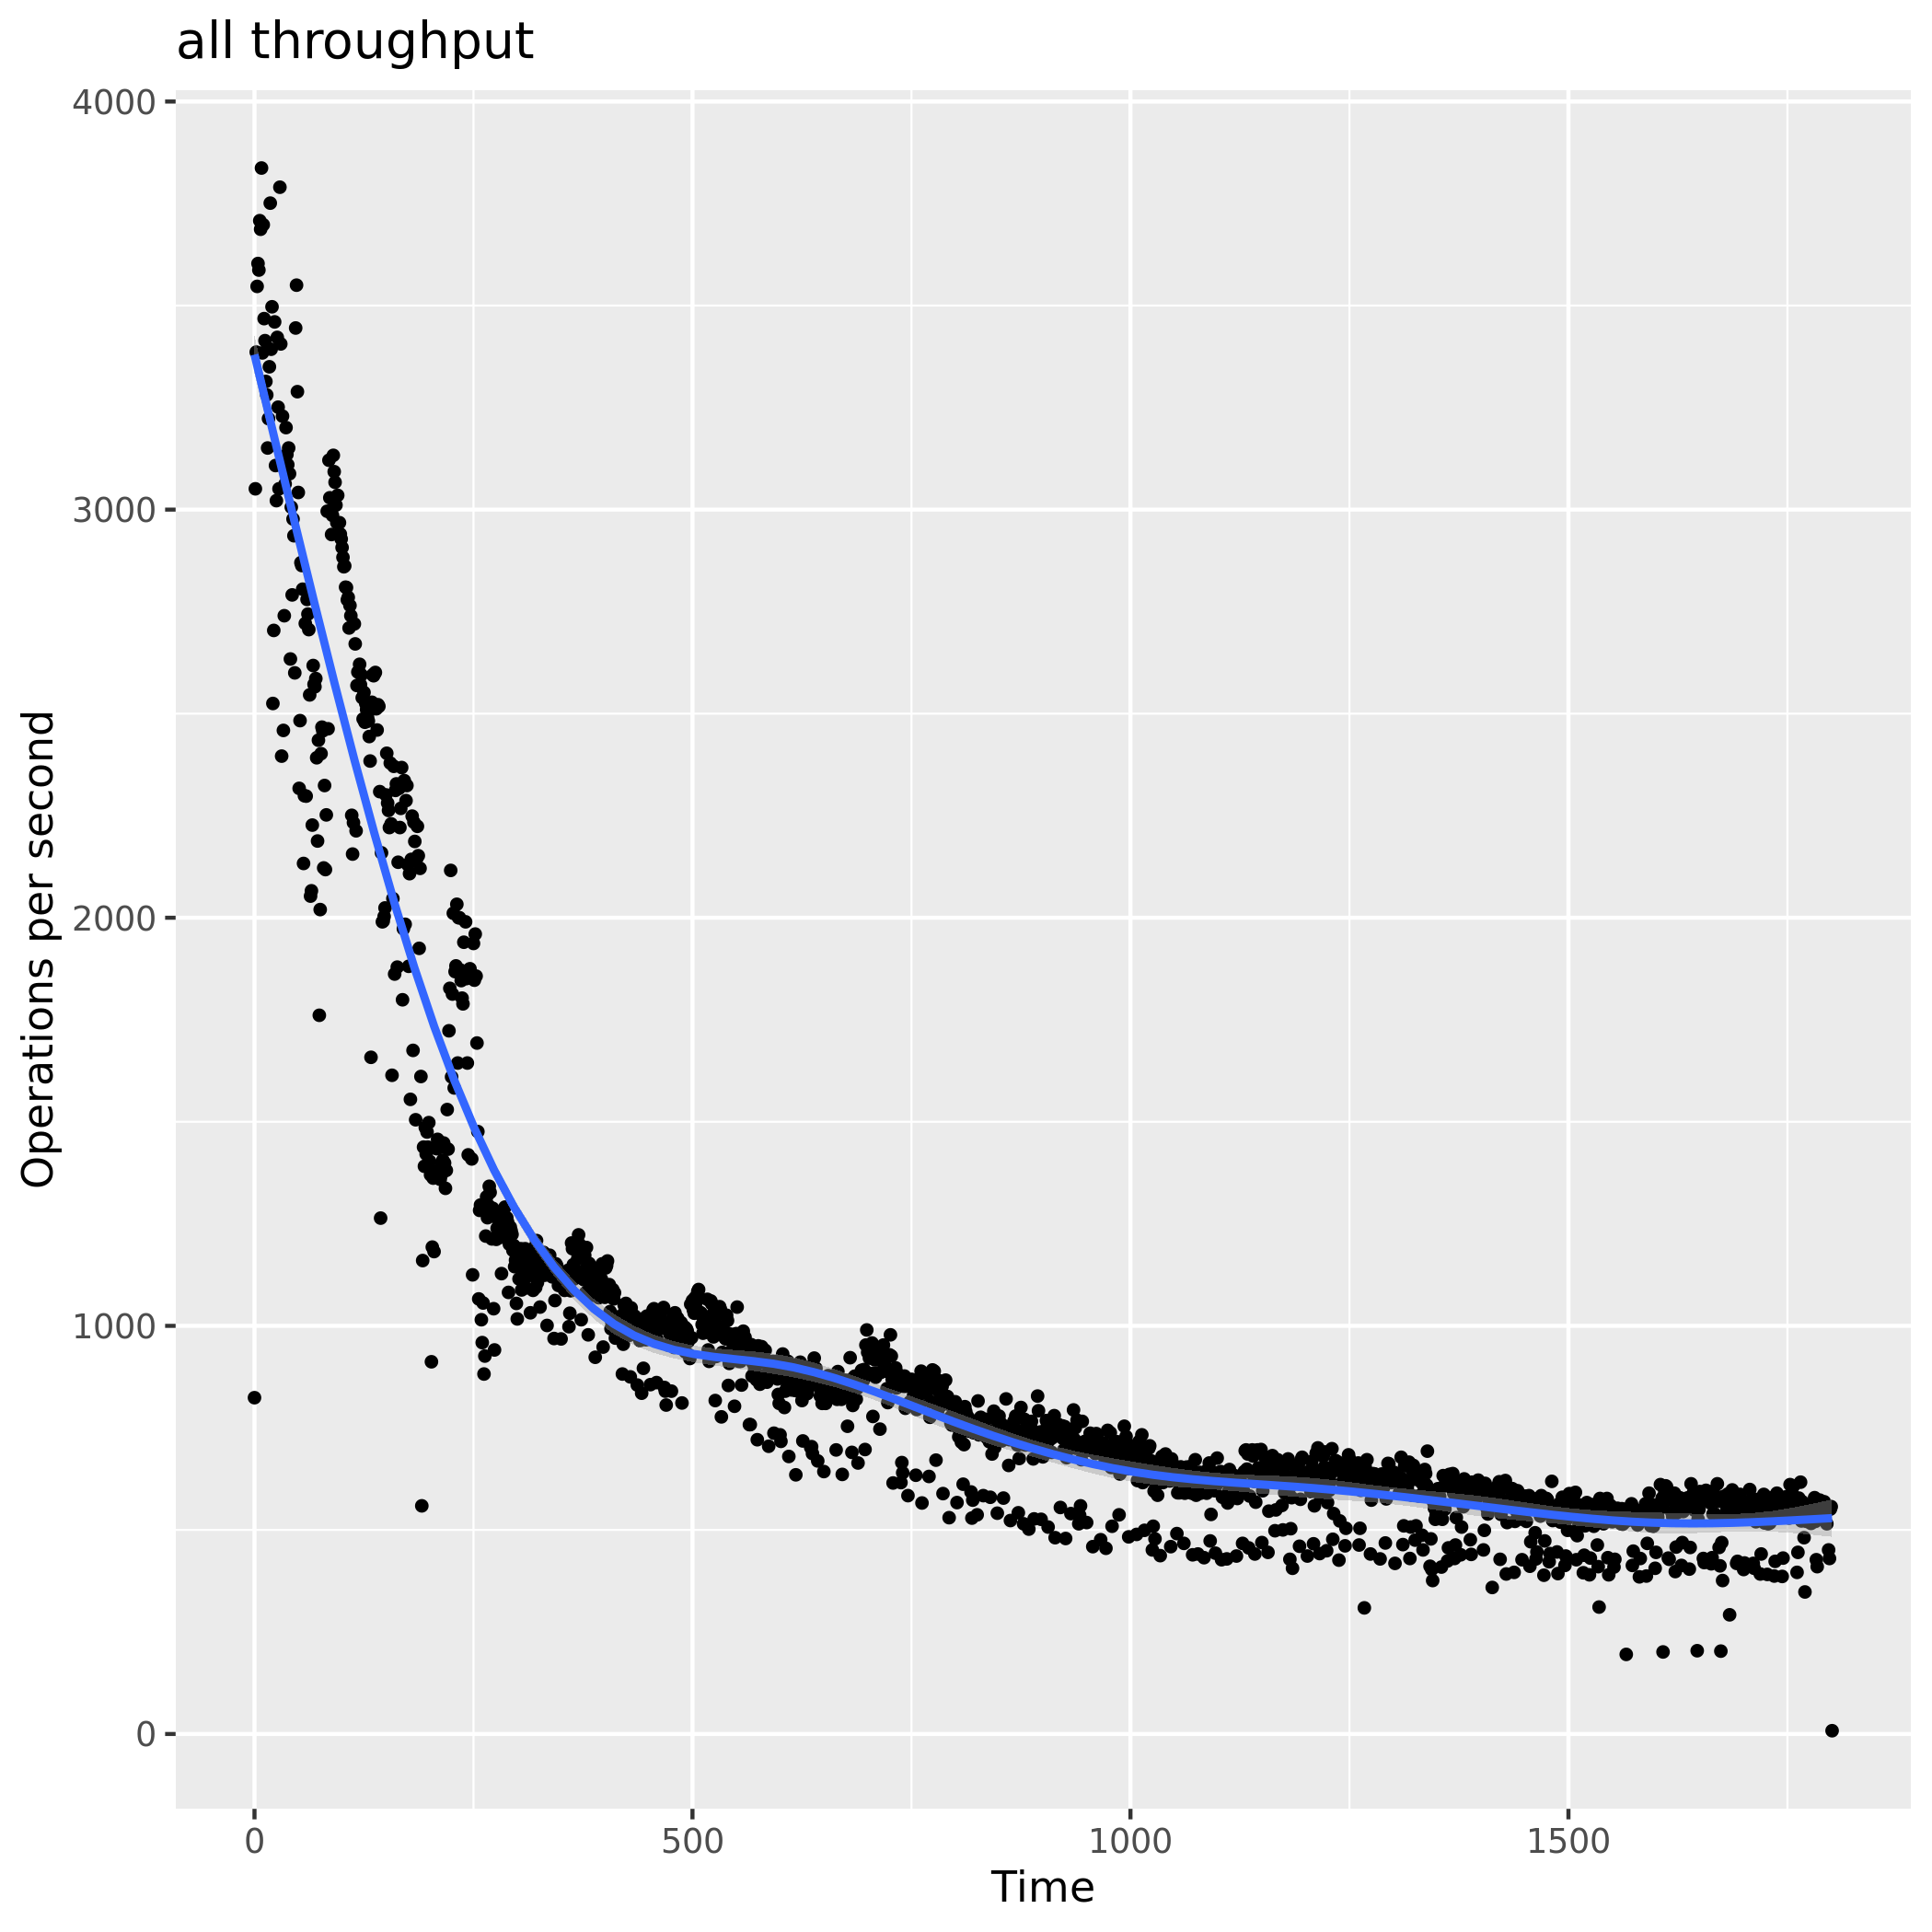
\includegraphics[width=0.5\textwidth]{RandomSlicing_Jumping_C0_write_heavy_throughput}
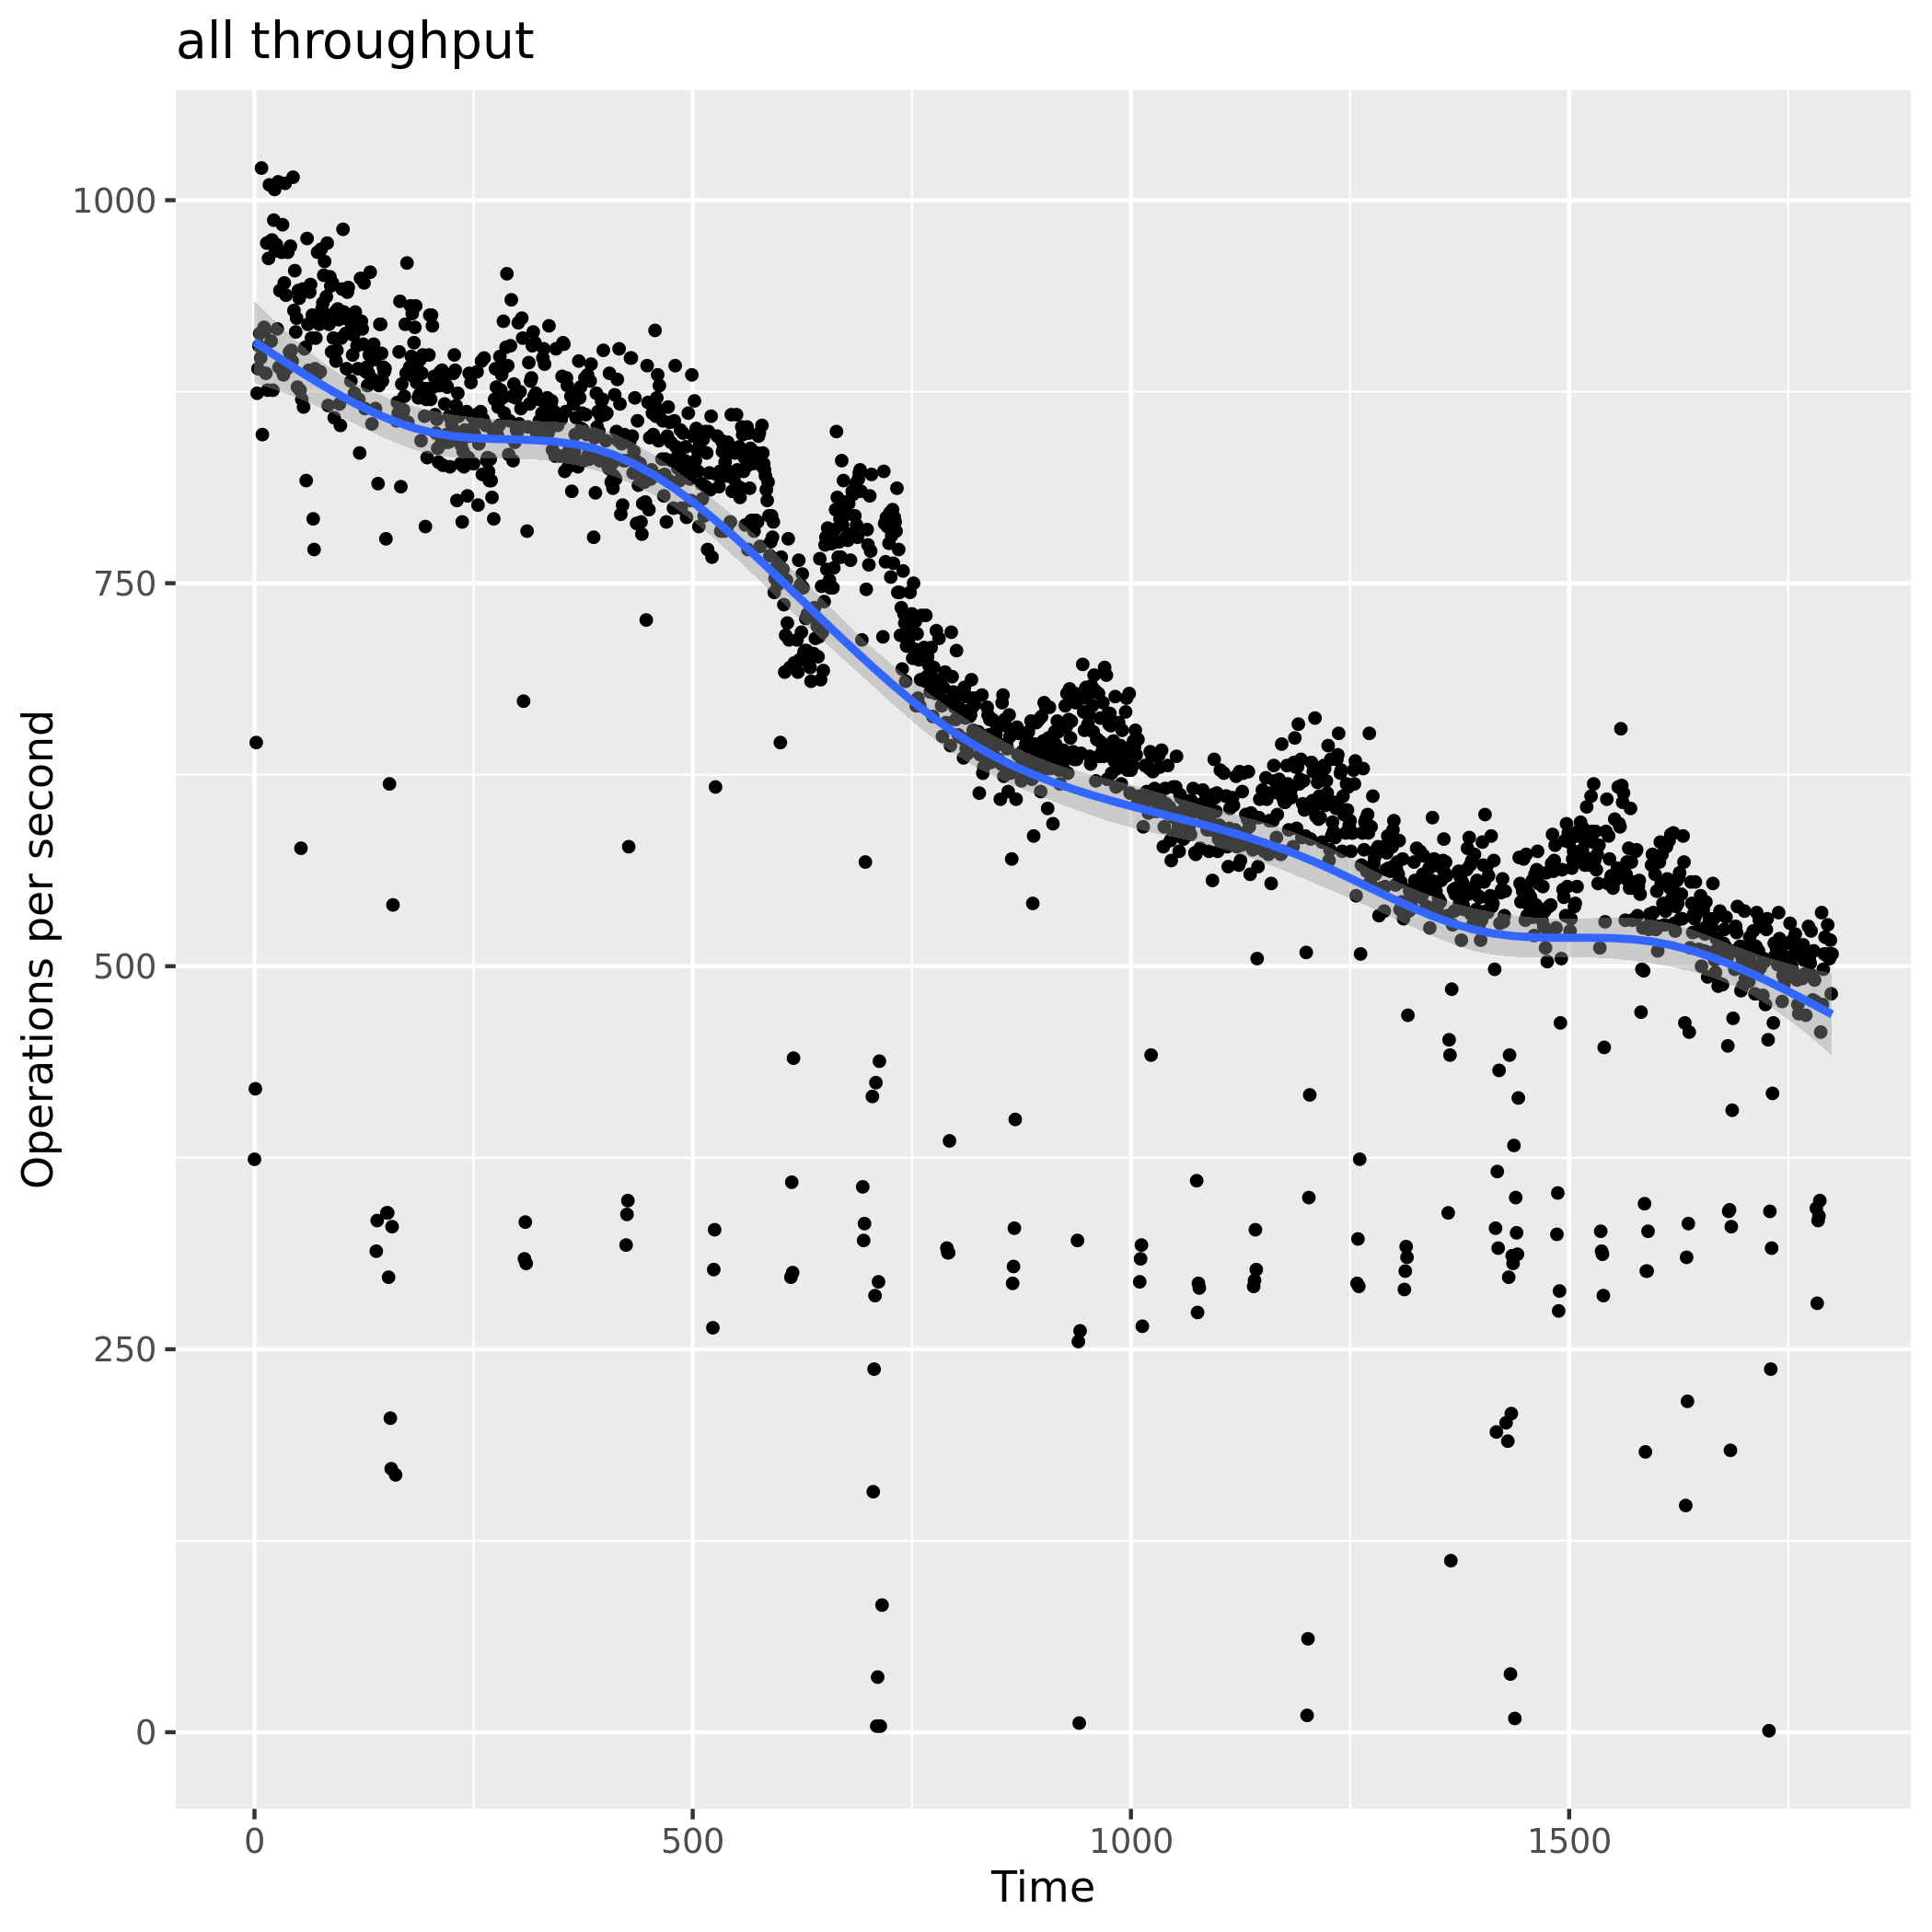
\includegraphics[width=0.5\textwidth]{RandomSlicing_Jumping_C2_write_heavy_throughput}
\caption[\ac{RS} with Ring Jumping Throughput Comparison]{\ac{RS} with Ring Jumping Throughput Comparison. Showing the throughput for \ac{RS} with Ring Jumping in C0 and C2 with write-heavy workload.}
\label{fig:throughput_random_jumping}
\end{figure}

In the dynamic benchmark runs the decrease in throughput after each configuration change is in accordance with the values measured for those configurations in the static run.
An exemplary visualization of the write-heavy dynamic run is shown in \cref{fig:random_slicing_jumping_dynamic}.
Just before the change from C0 to C1 the throughput is at about 1000 operations per second which is the same as just before the change from C1 to C2.
At the end of the run the throughput decreased to about 550 operations per second.
There is a clear edge in the latency plot at the 600s and 1200s mark but there is no visible phase of disruption which implies that there is not a long phase of handoff operations.
\begin{figure}
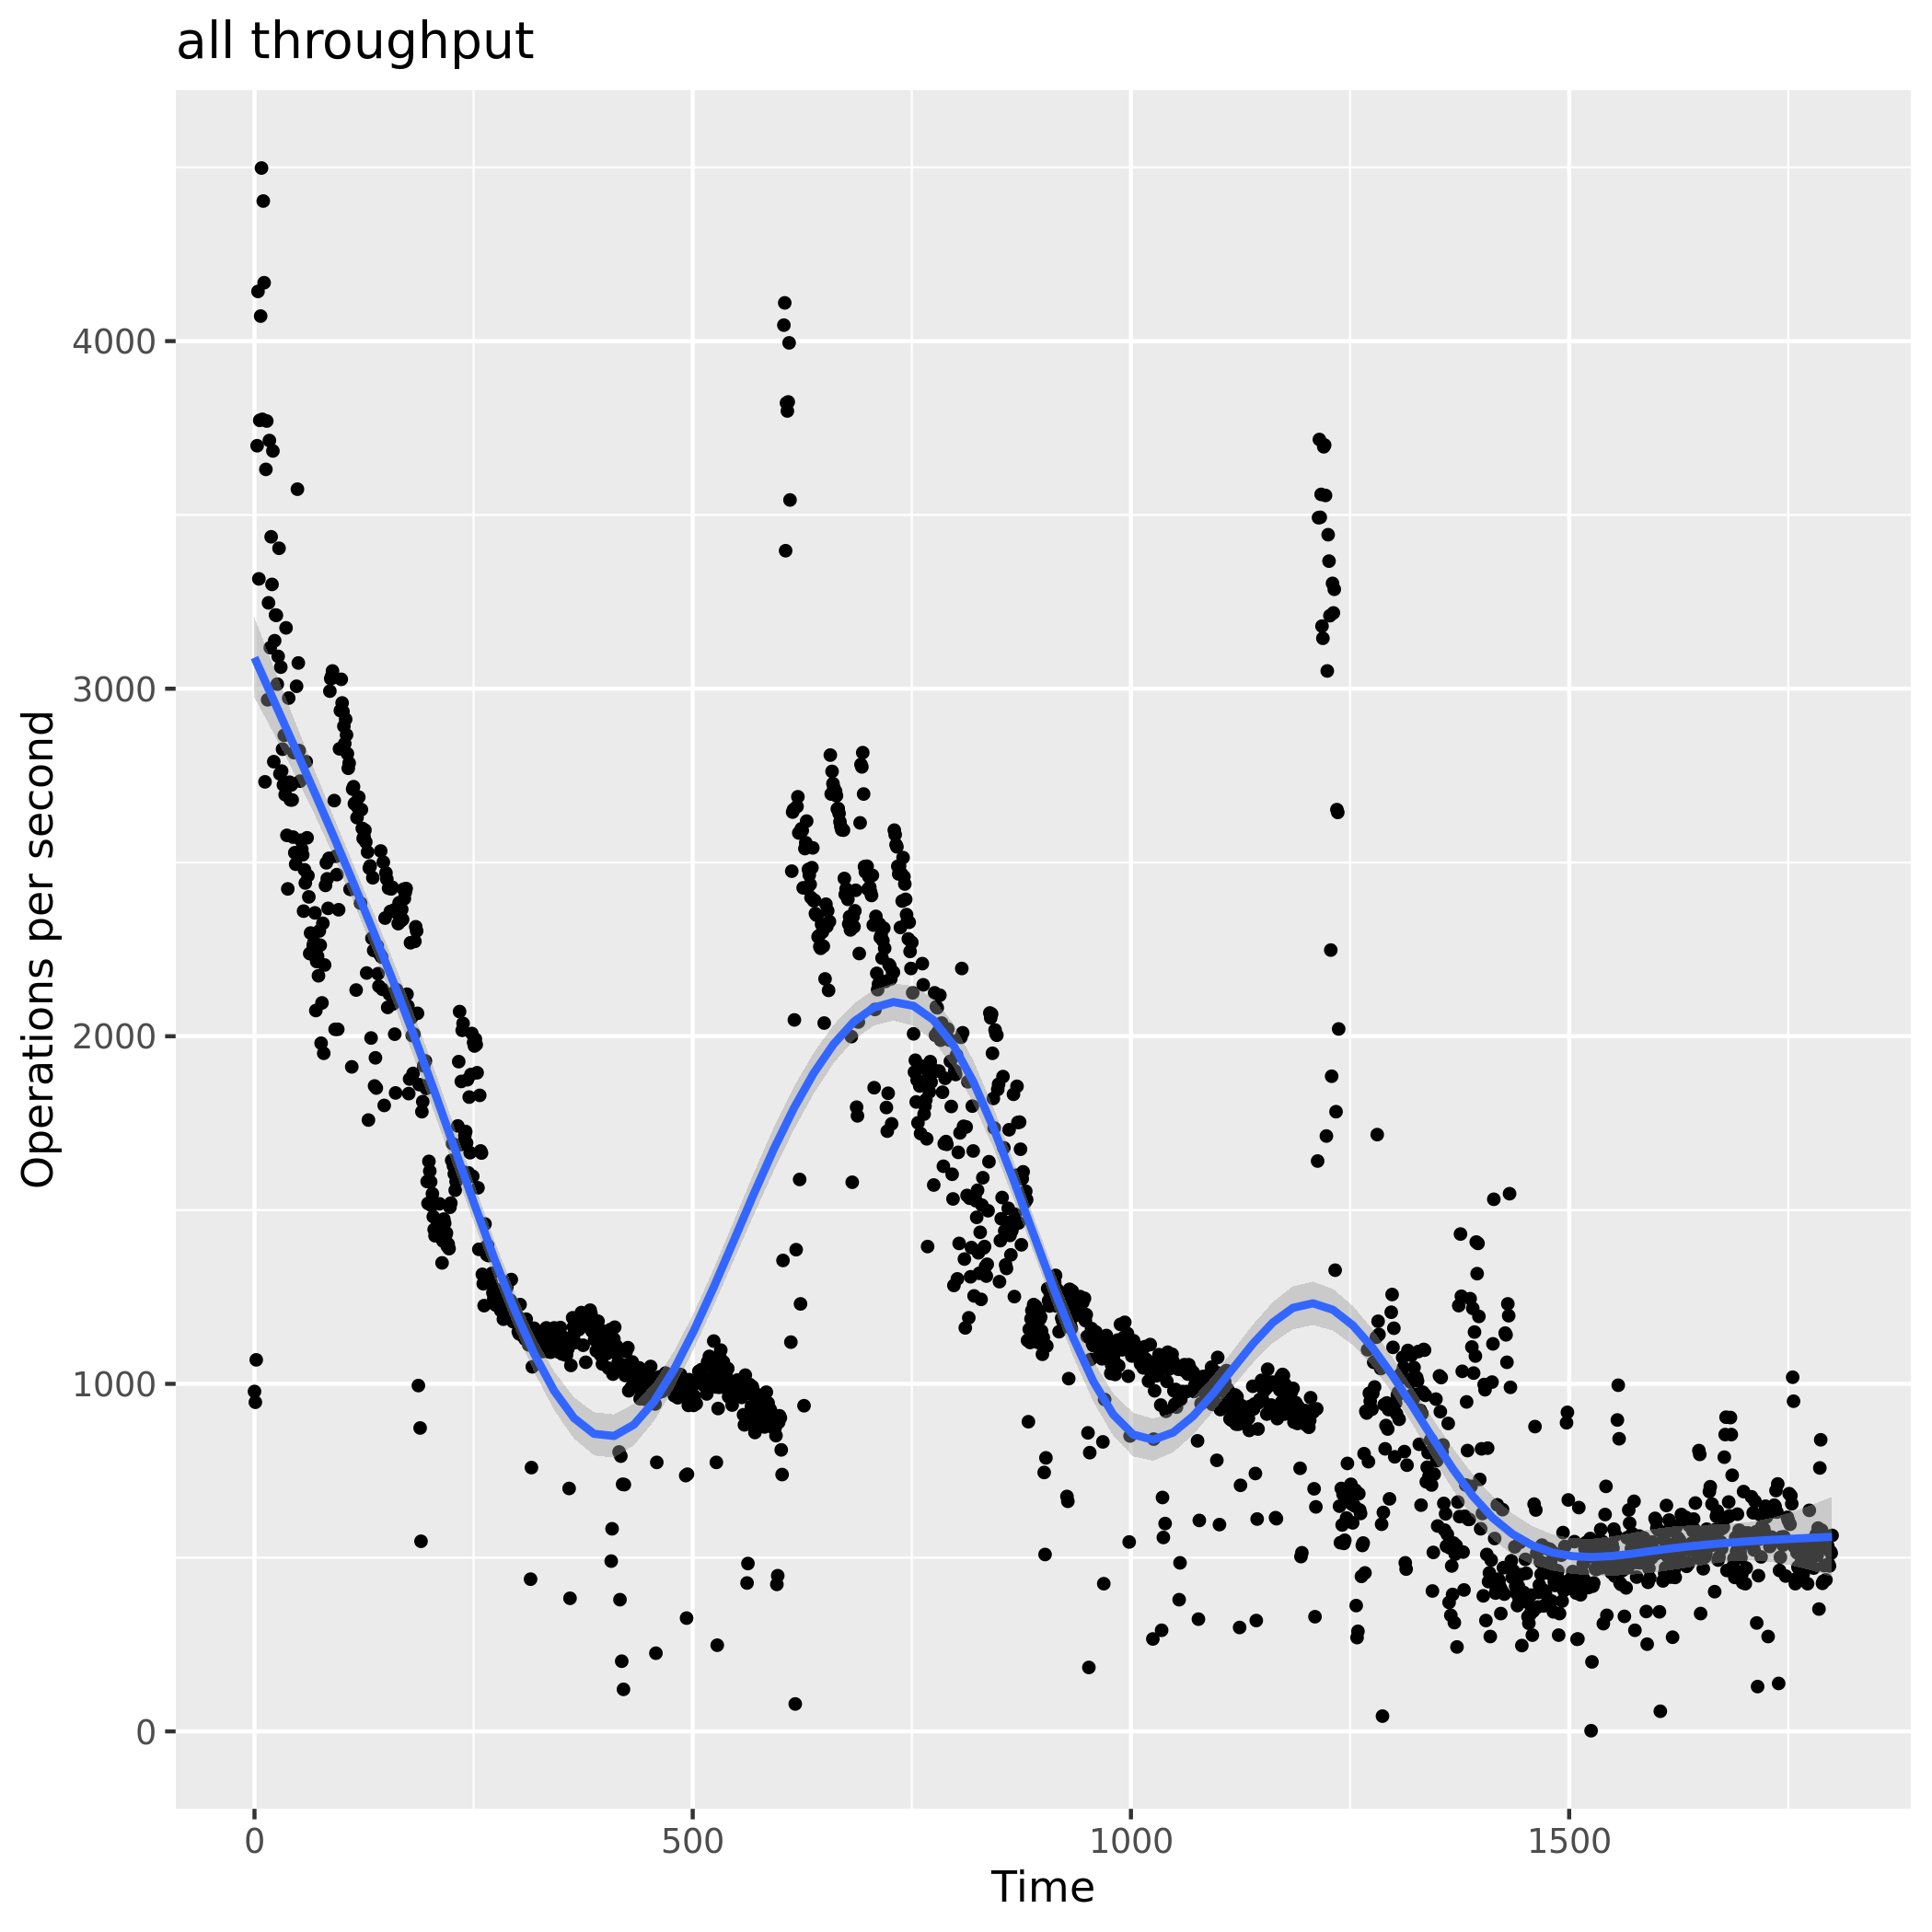
\includegraphics[width=0.5\textwidth]{RandomSlicing_Jumping_dynamic_write_heavy_throughput}
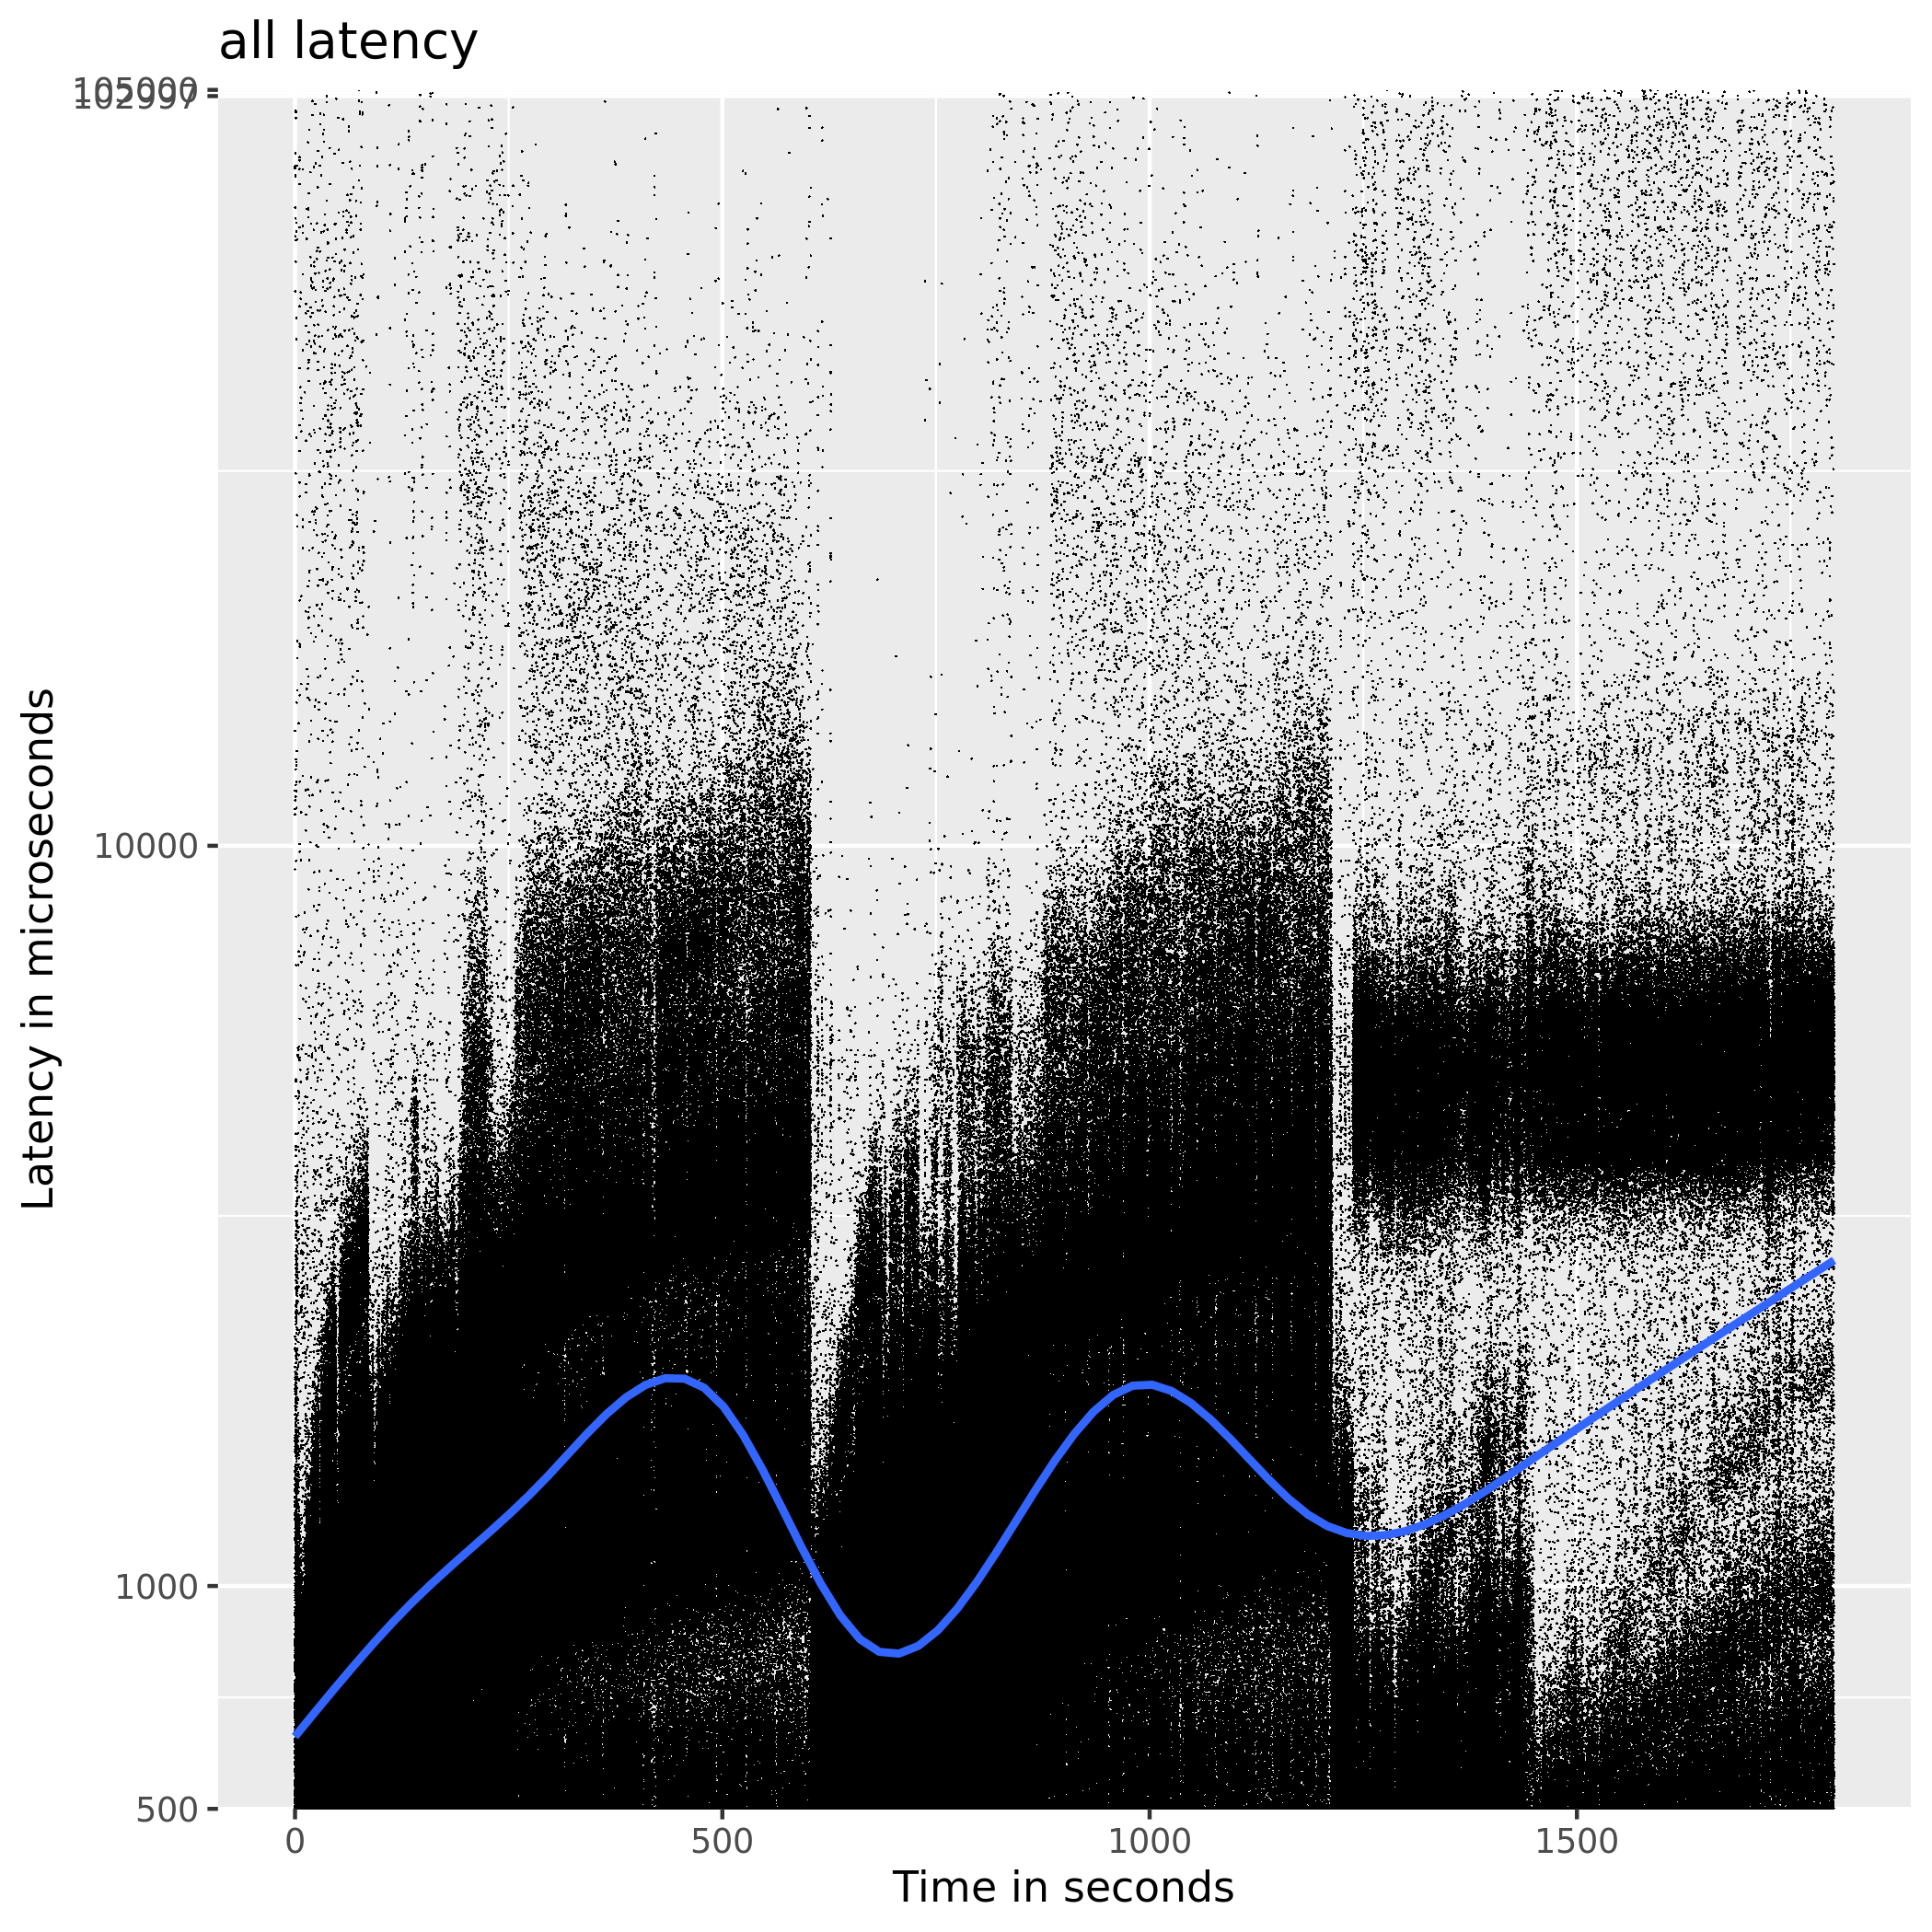
\includegraphics[width=0.5\textwidth]{RandomSlicing_Jumping_dynamic_write_heavy_latency}
\caption[Dynamic Run with \ac{RS} and Ring Jumping]{Dynamic Runs with \ac{RS} and Ring Jumping.}
\label{fig:random_slicing_jumping_dynamic}
\end{figure}

Regarding the divergence from optimal load balance with \ac{RS} and Ring Jumping there is an absolute overall average divergence for key load of 0.0303095841515983, for put load of 0.036558287305248, and for get load of 0.03657058797636.
Ignoring C0 with exactly three sections the highest divergence is measured in the dynamic configuration and the lowest is measured in C1.
This is quite intuitive as in C1 there are not many section and the sections are of a reasonable size while in the dynamic run the keys are potentially to the wrong node initially and will only be balanced after the repair operations are started for each key.

\subsection{Random Slicing Random}
Apart from one abnormal run there are no significant differences between read-heavy and write-heavy runs with respect to the throughput but a slightly higher rate for read-heavy workloads at the start.
A comparison between the throuput in C0 and C2 is shown in \cref{fig:throughput_random_slicing_random}.
In configuration C0 the throughput starts at about 2800 operations per second, steeply declines to 1000 operations per second at about 500s and then slowly decreases to 500 operations per second.
The read-heavy run in C1 results in about the same throughput plot, however it ends at about 600 operations per second.
The write-heavy run in C1 on the other hand shows an anomaly of a throughput spike at about 1300s and a sharp edge in the latency plot.
Those anomalies can be seen in \cref{fig:random_slicing_random_anomaly}.
\begin{figure}
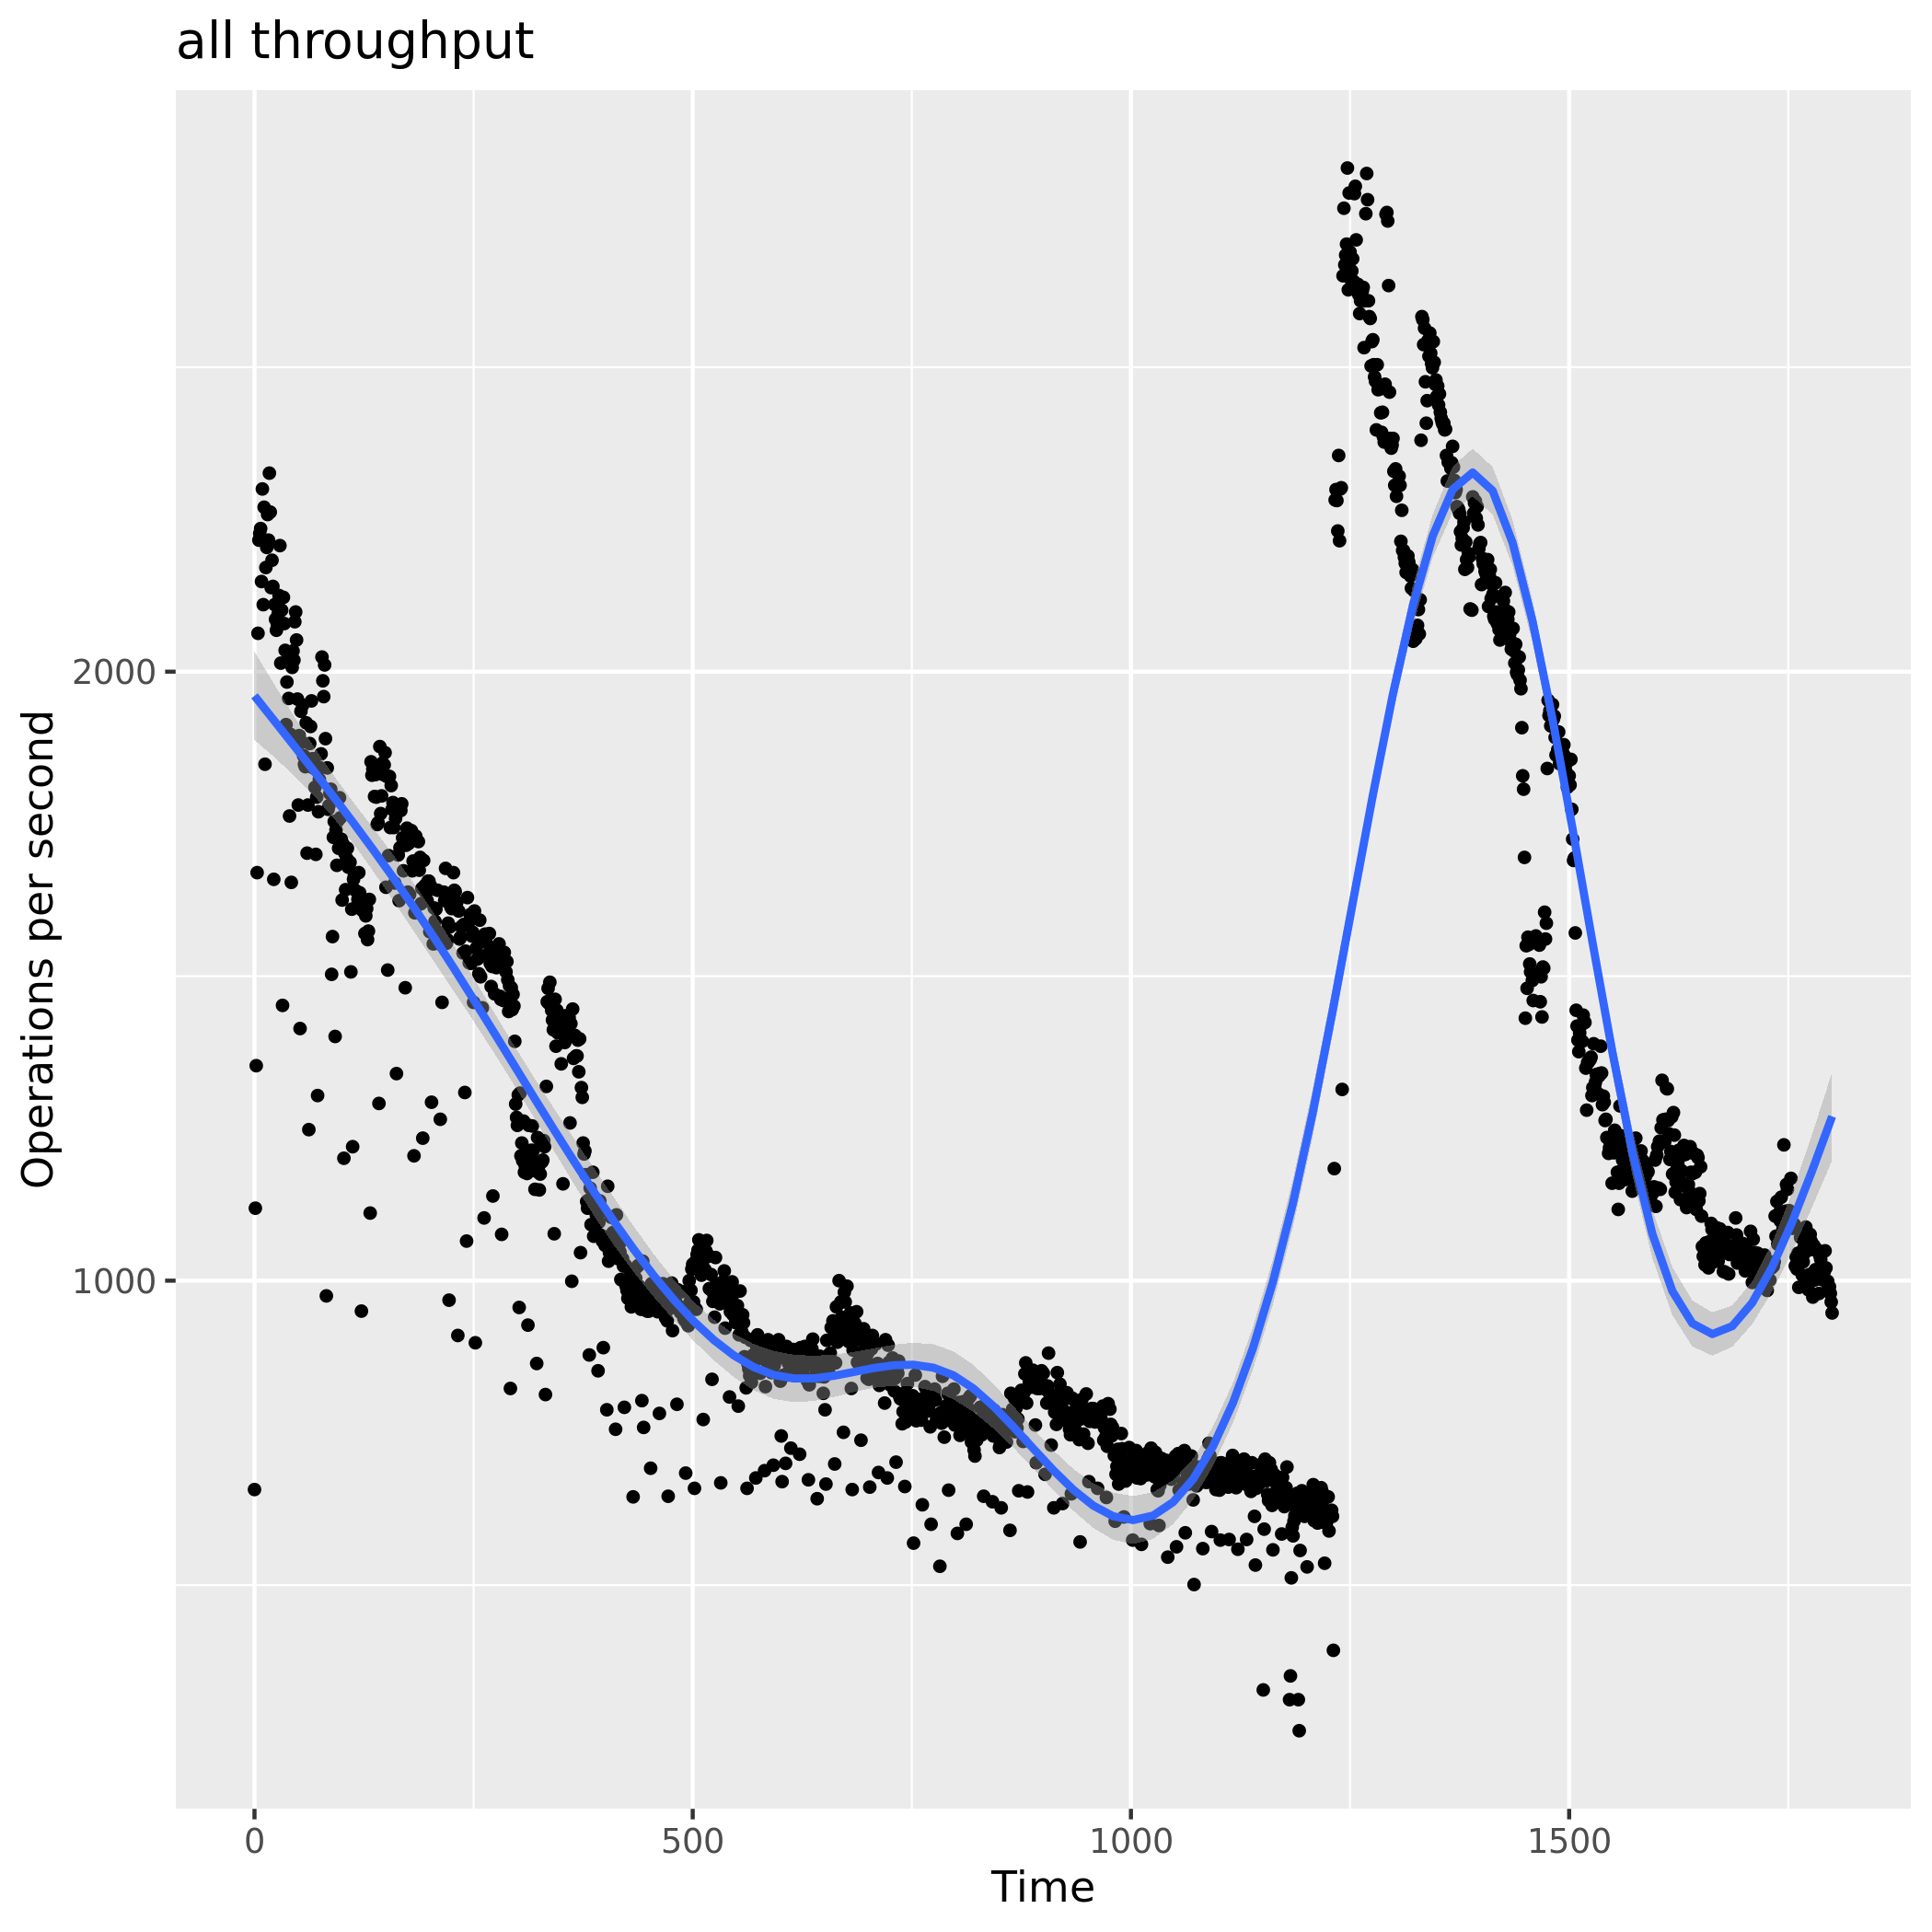
\includegraphics[width=0.5\textwidth]{RandomSlicing_Random_C1_write_heavy_throughput}
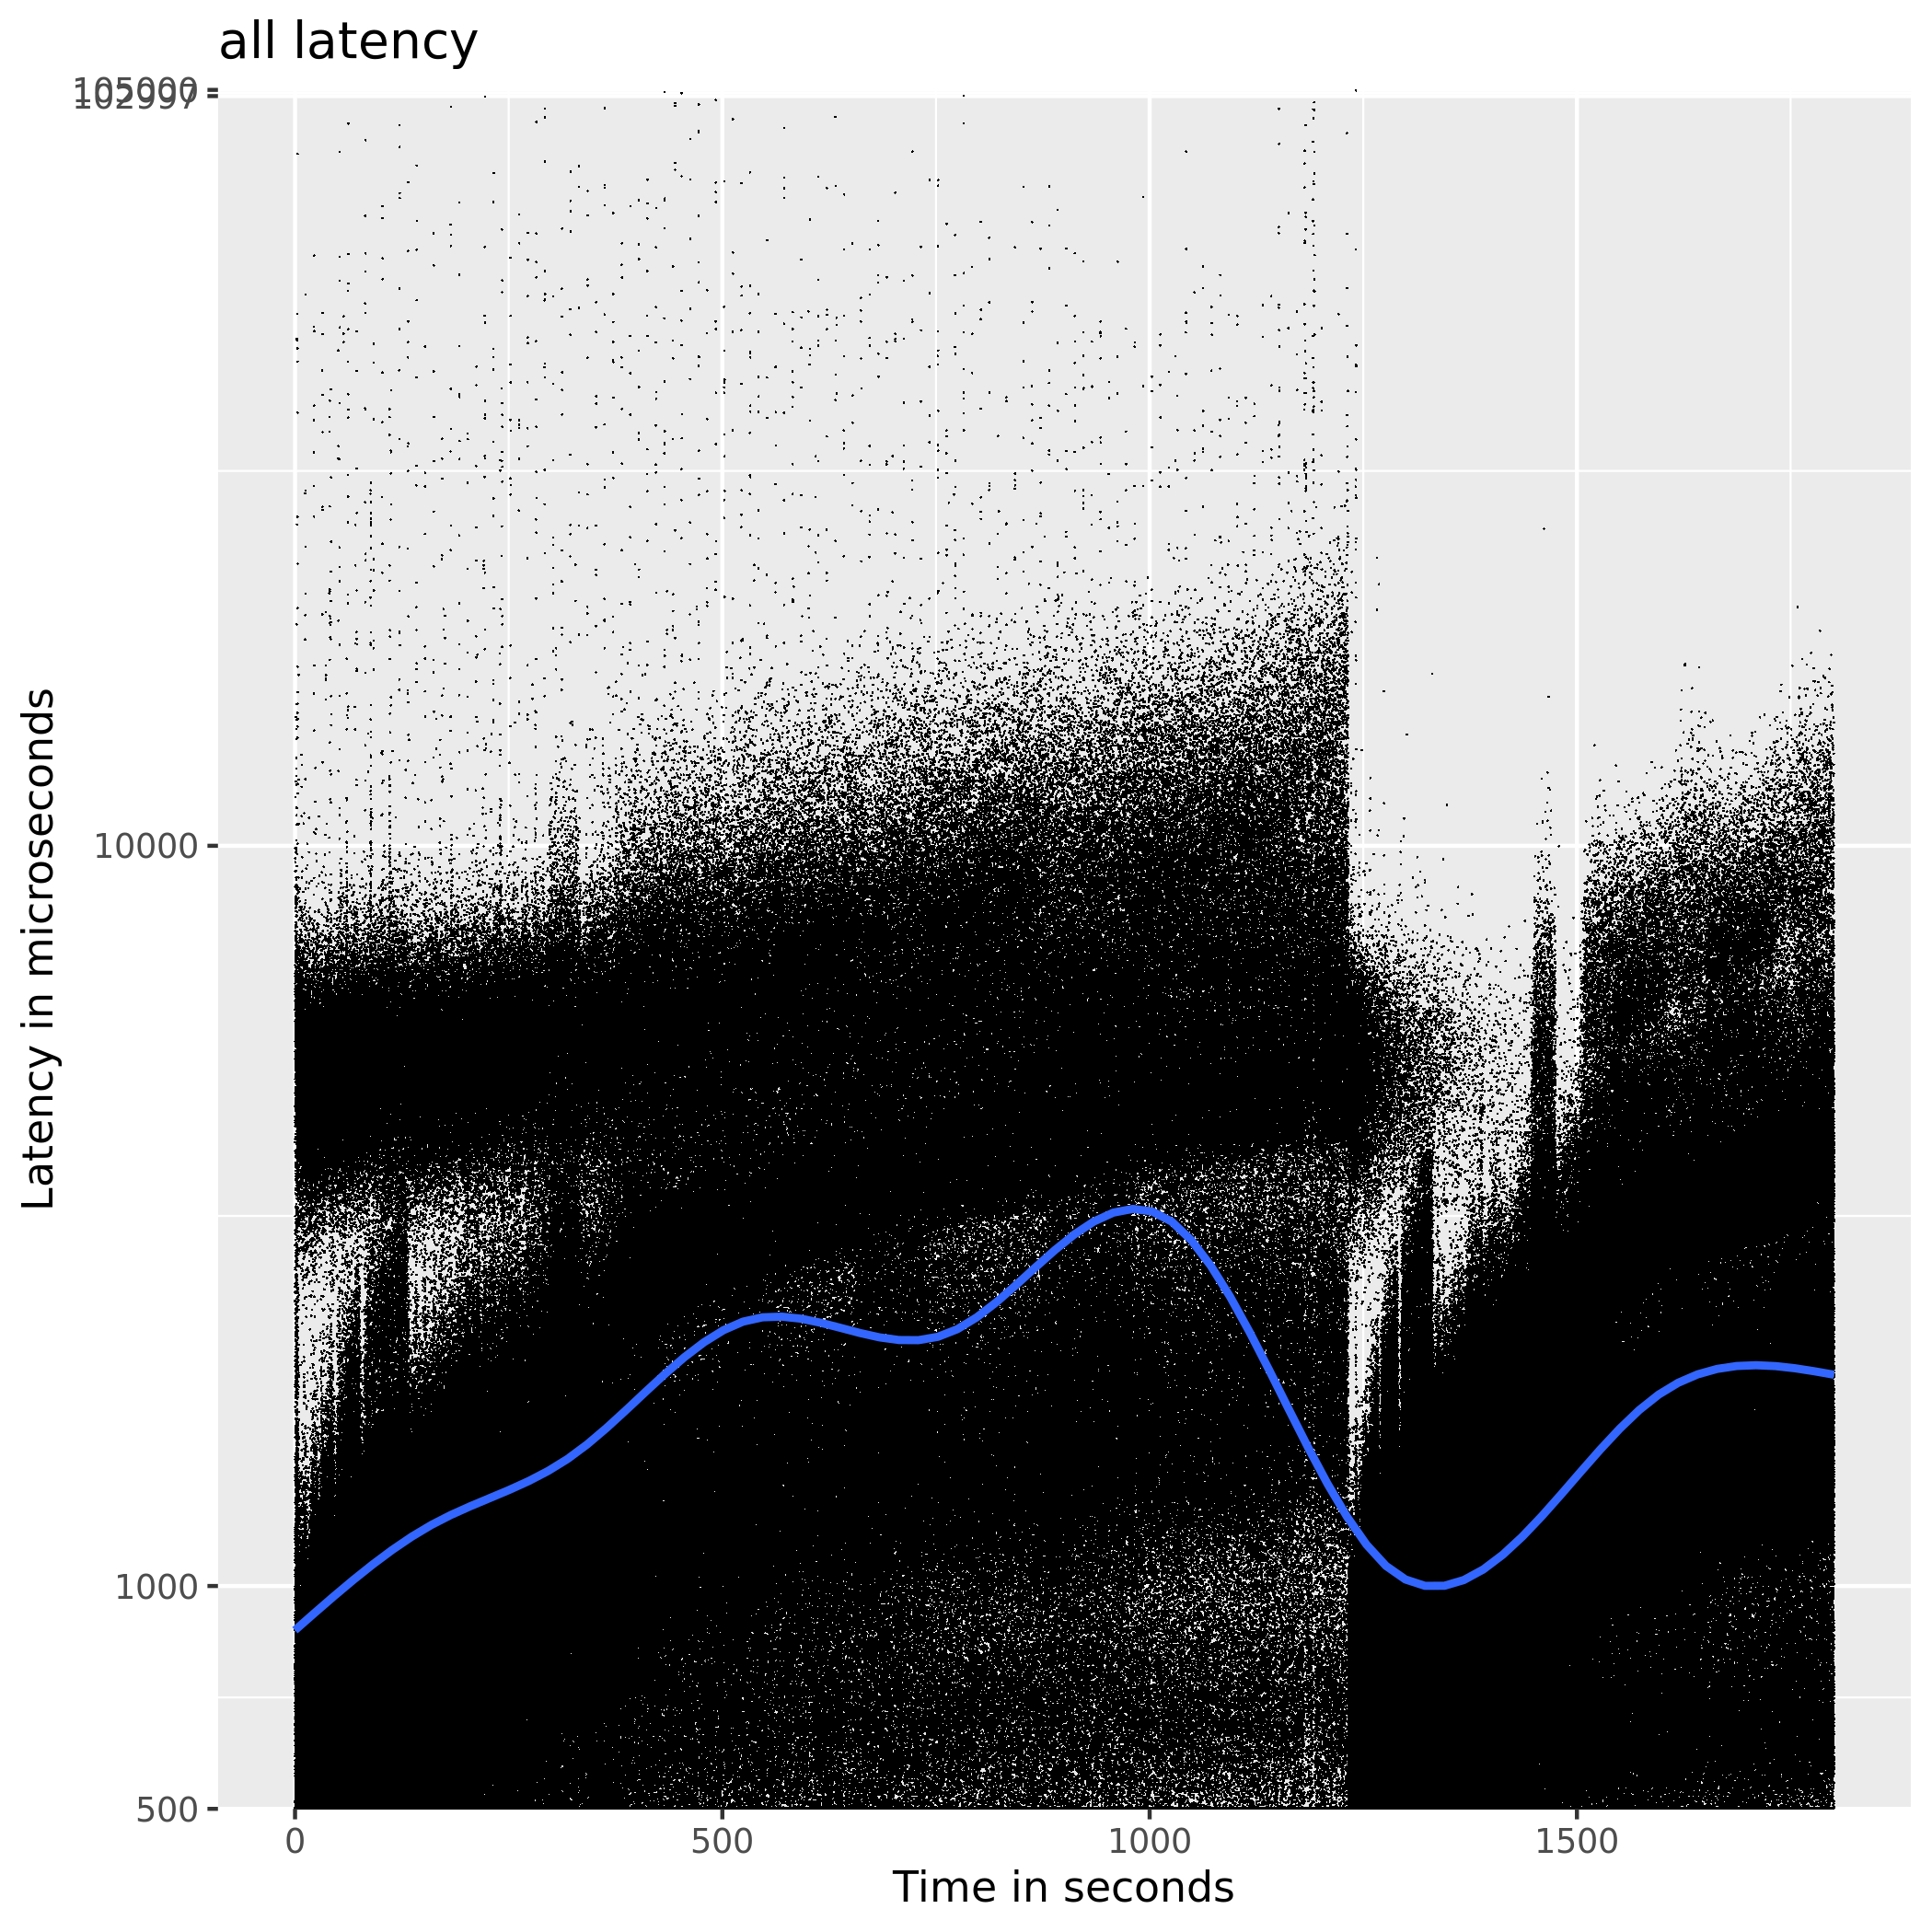
\includegraphics[width=0.5\textwidth]{RandomSlicing_Random_C1_write_heavy_latency}
\caption[\ac{RS} with Ramdom Replication Anomaly]{\ac{RS} with Ramdom Replication Anomaly. Even though the configuration is supposed to be static the throughput and latency plots show signs of a cluster change at 1300s.}
\label{fig:random_slicing_random_anomaly}
\end{figure}
These are signs that imply a cluster change and handoff started at that time according to all dynamic runs.
Assuming this is the case this run has to be excluded from the results.
There is a clear decline in performance when looking at configuration C2 with seven as the throughput starts at 750 operations per second and declines to 500 operations per second.
\begin{figure}
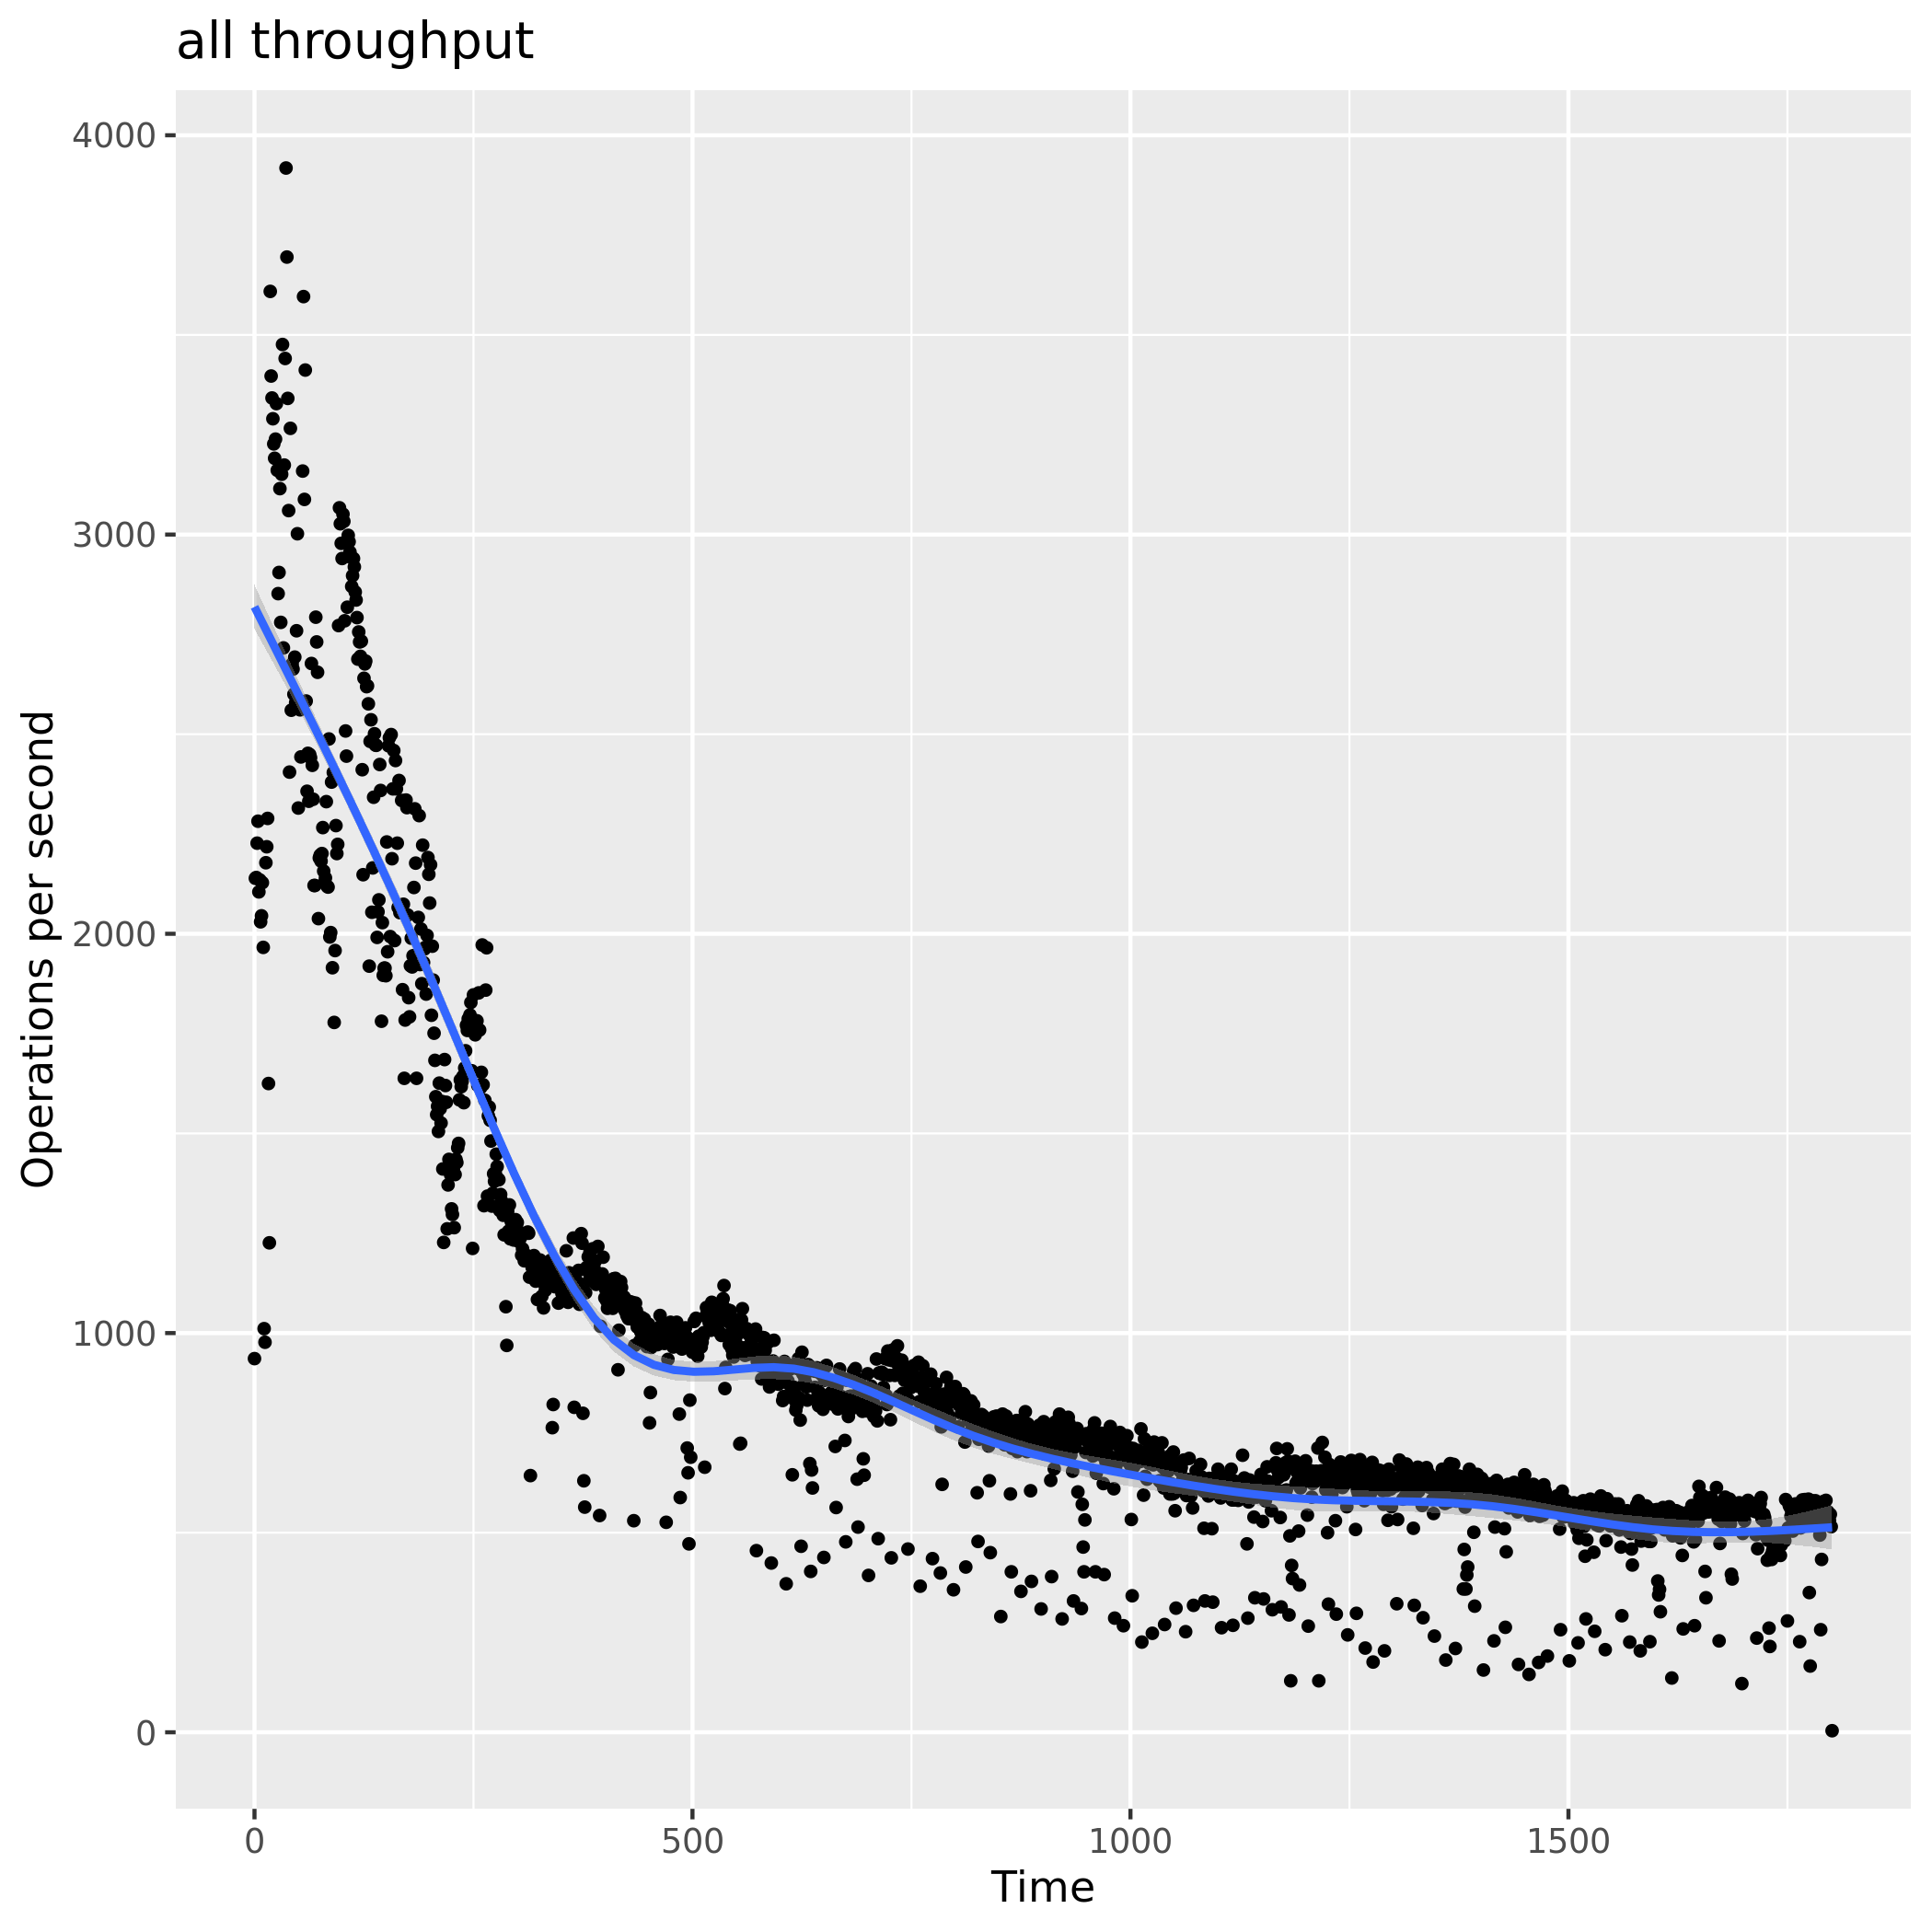
\includegraphics[width=0.5\textwidth]{RandomSlicing_Random_C0_write_heavy_throughput}
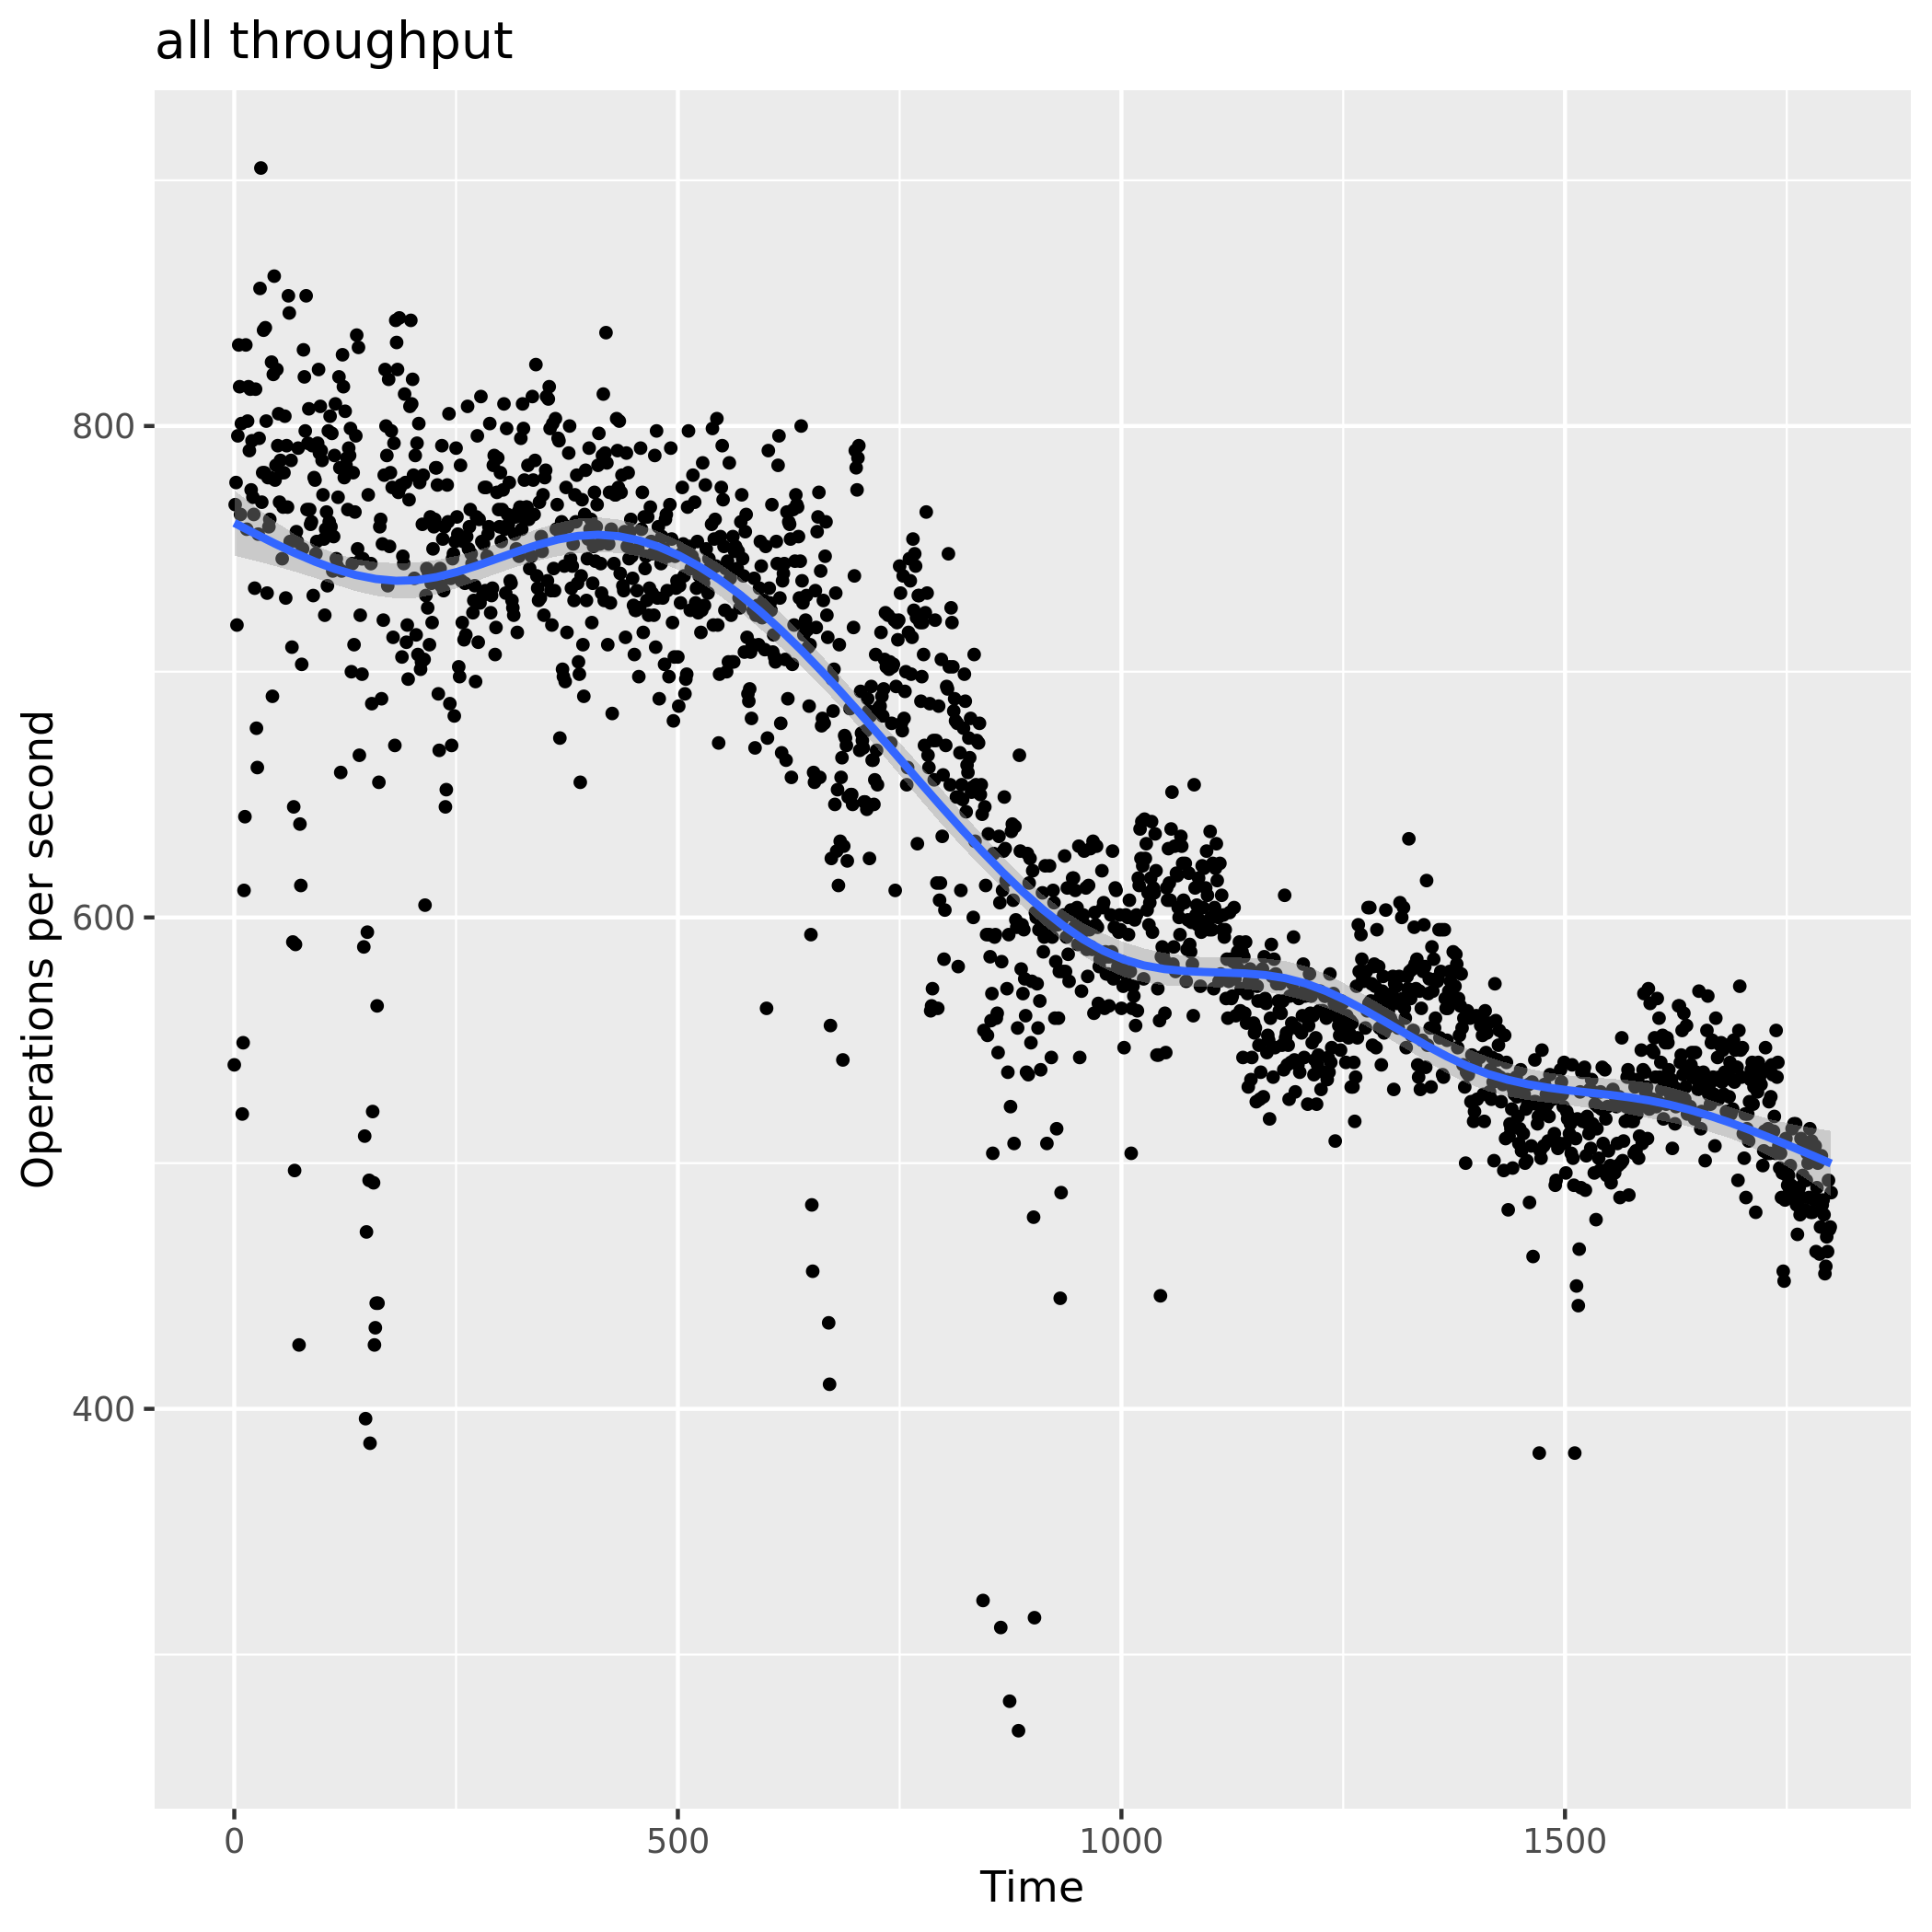
\includegraphics[width=0.5\textwidth]{RandomSlicing_Random_C2_write_heavy_throughput}
\caption[\ac{RS} with Ramdom Replication Throughput]{\ac{RS} with Ramdom Replication Throughput. Comparison of the throughput in C0 and C2.}
\label{fig:throughput_random_slicing_random}
\end{figure}

In the dynamic runs there seems to be a big difference in how the cluster changes are handled.
While the throughput seems to be quite similar in the sense that the second cluster change seems to have no big influence on the throughput the latency shows quite different images.
The latency plots of both workloads can be seen in \cref{fig:random_slicing_random_dynamic_latency}.
For the read-heavy workload there is an initial disruption at 600s and 1200s followed by a few smaller disruptions.
For the write-heavy workload there is a periodical occurrence of bigger disruptions starting at 600s and lasting up until 1000s.
These periodic disruptions do not show up as strongly after the second cluster change.
\begin{figure}
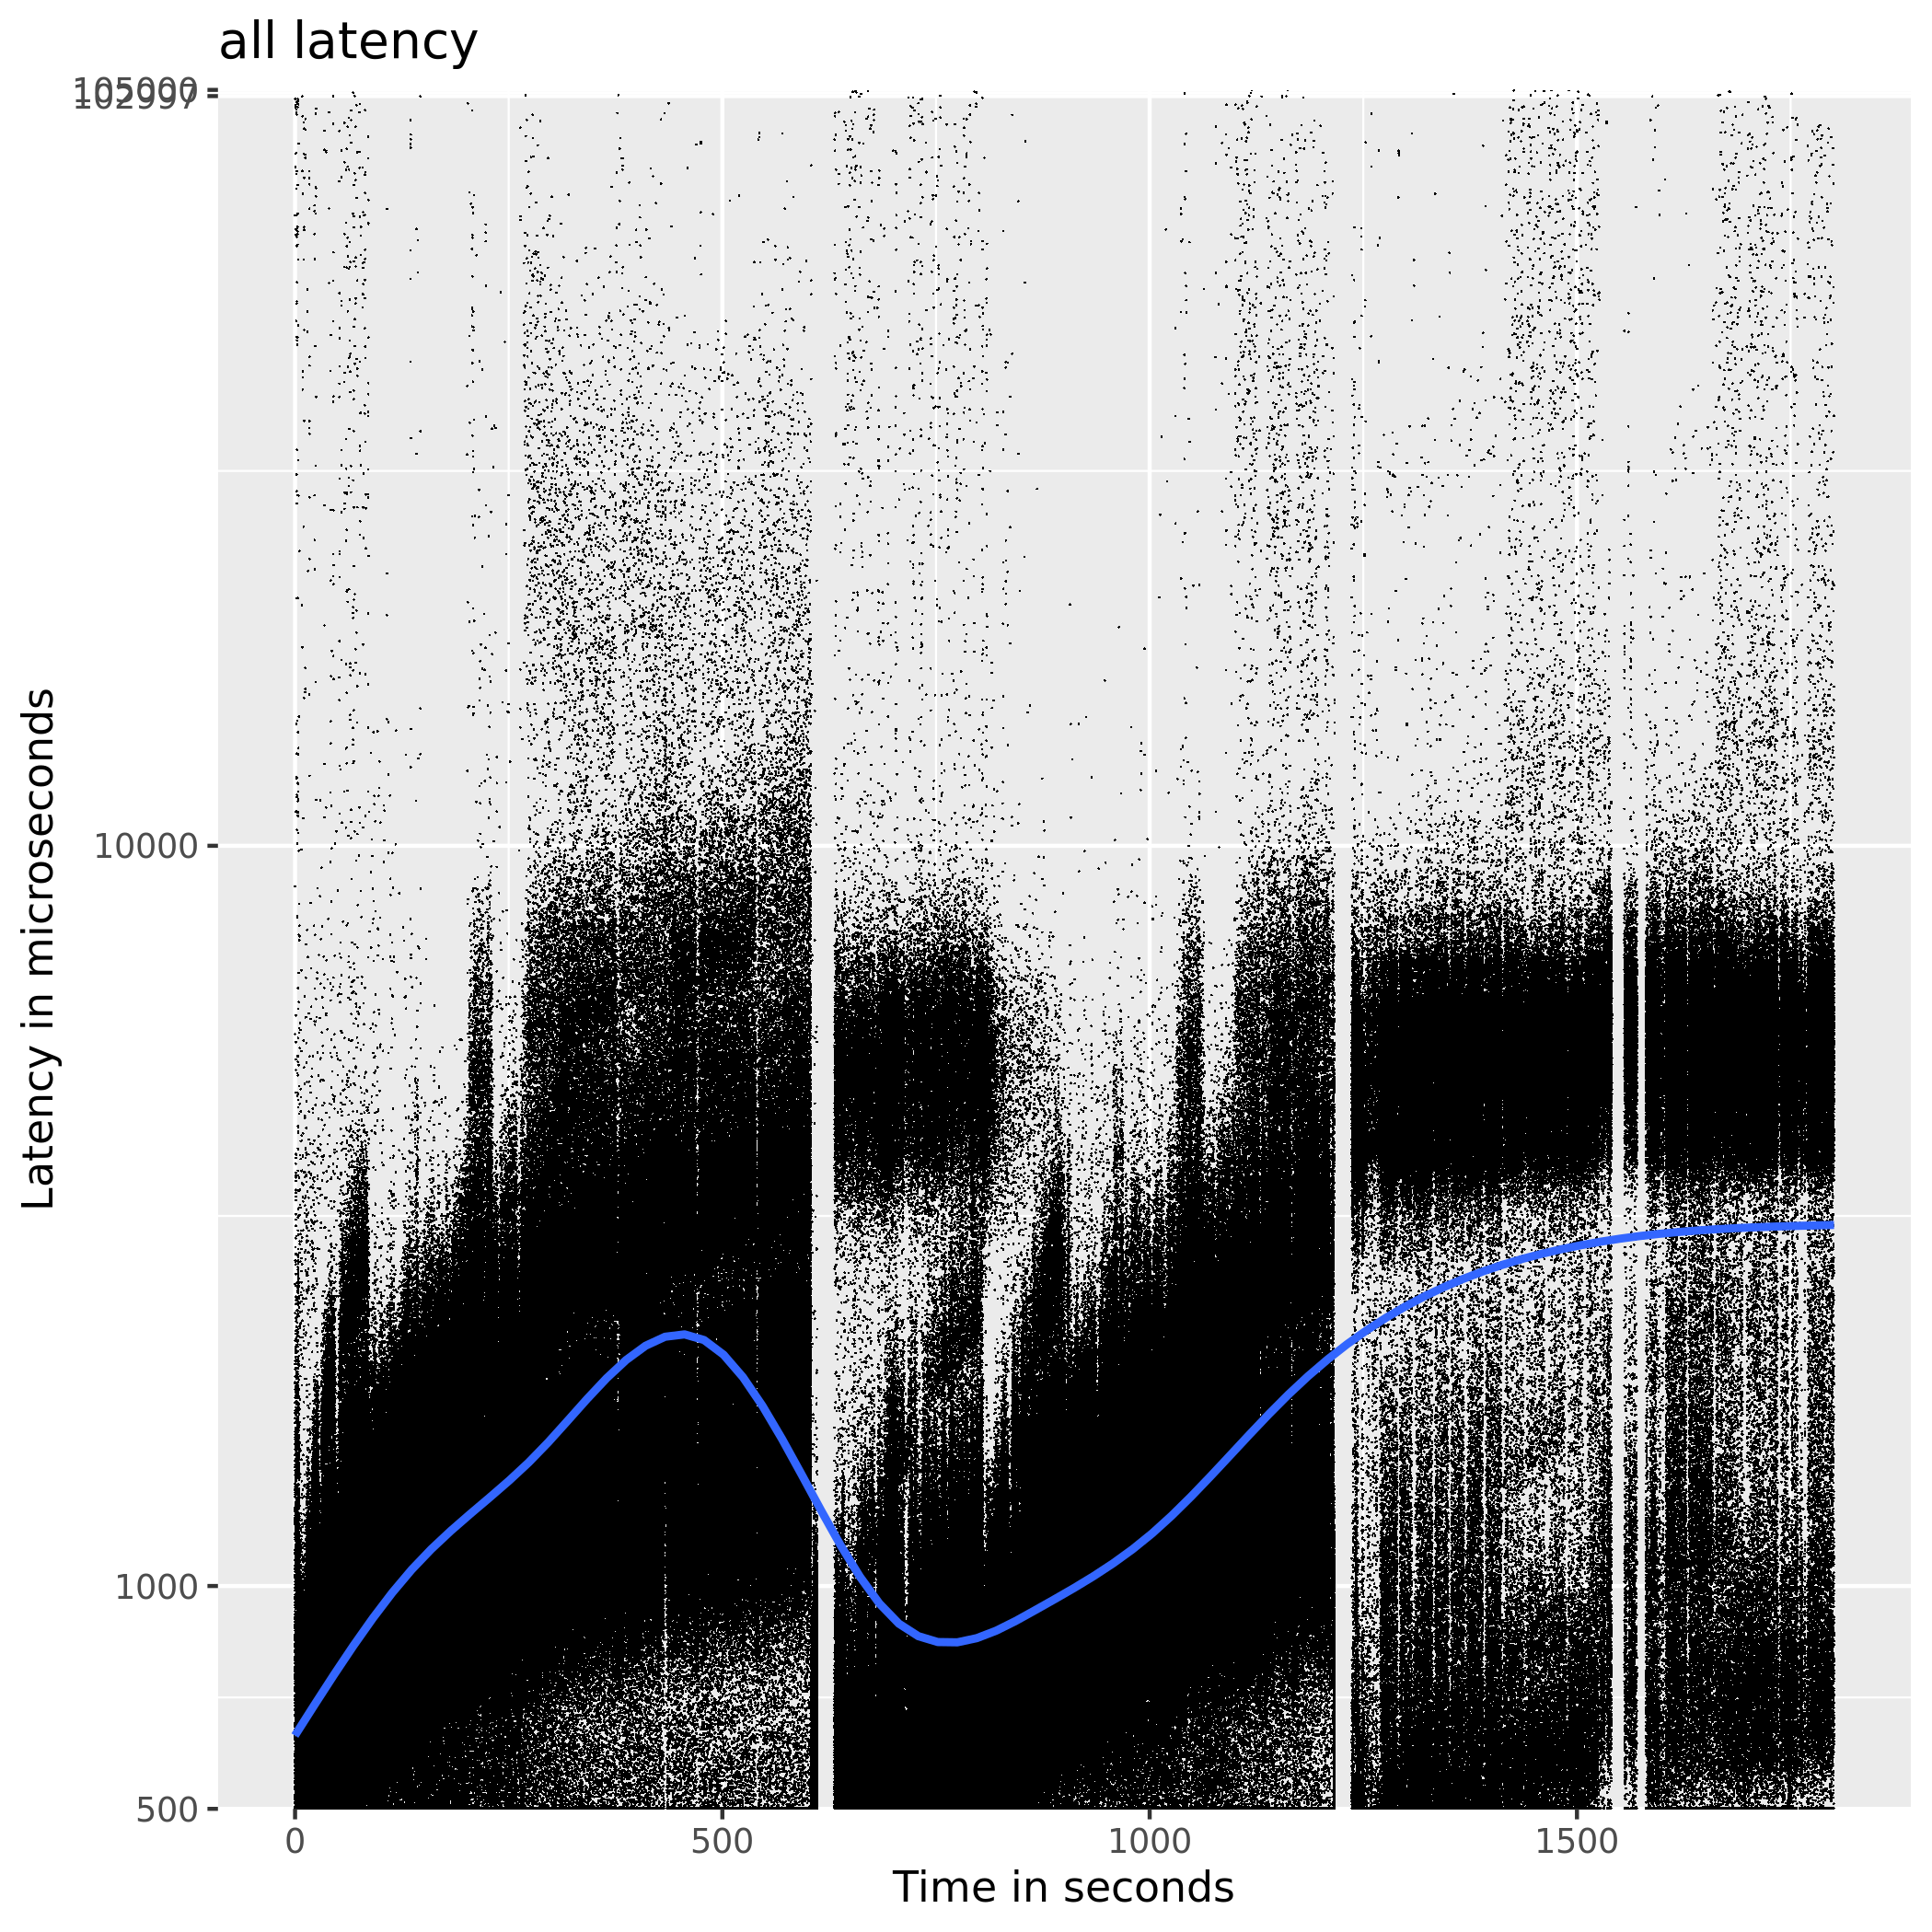
\includegraphics[width=0.5\textwidth]{RandomSlicing_Random_dynamic_read_heavy_latency}
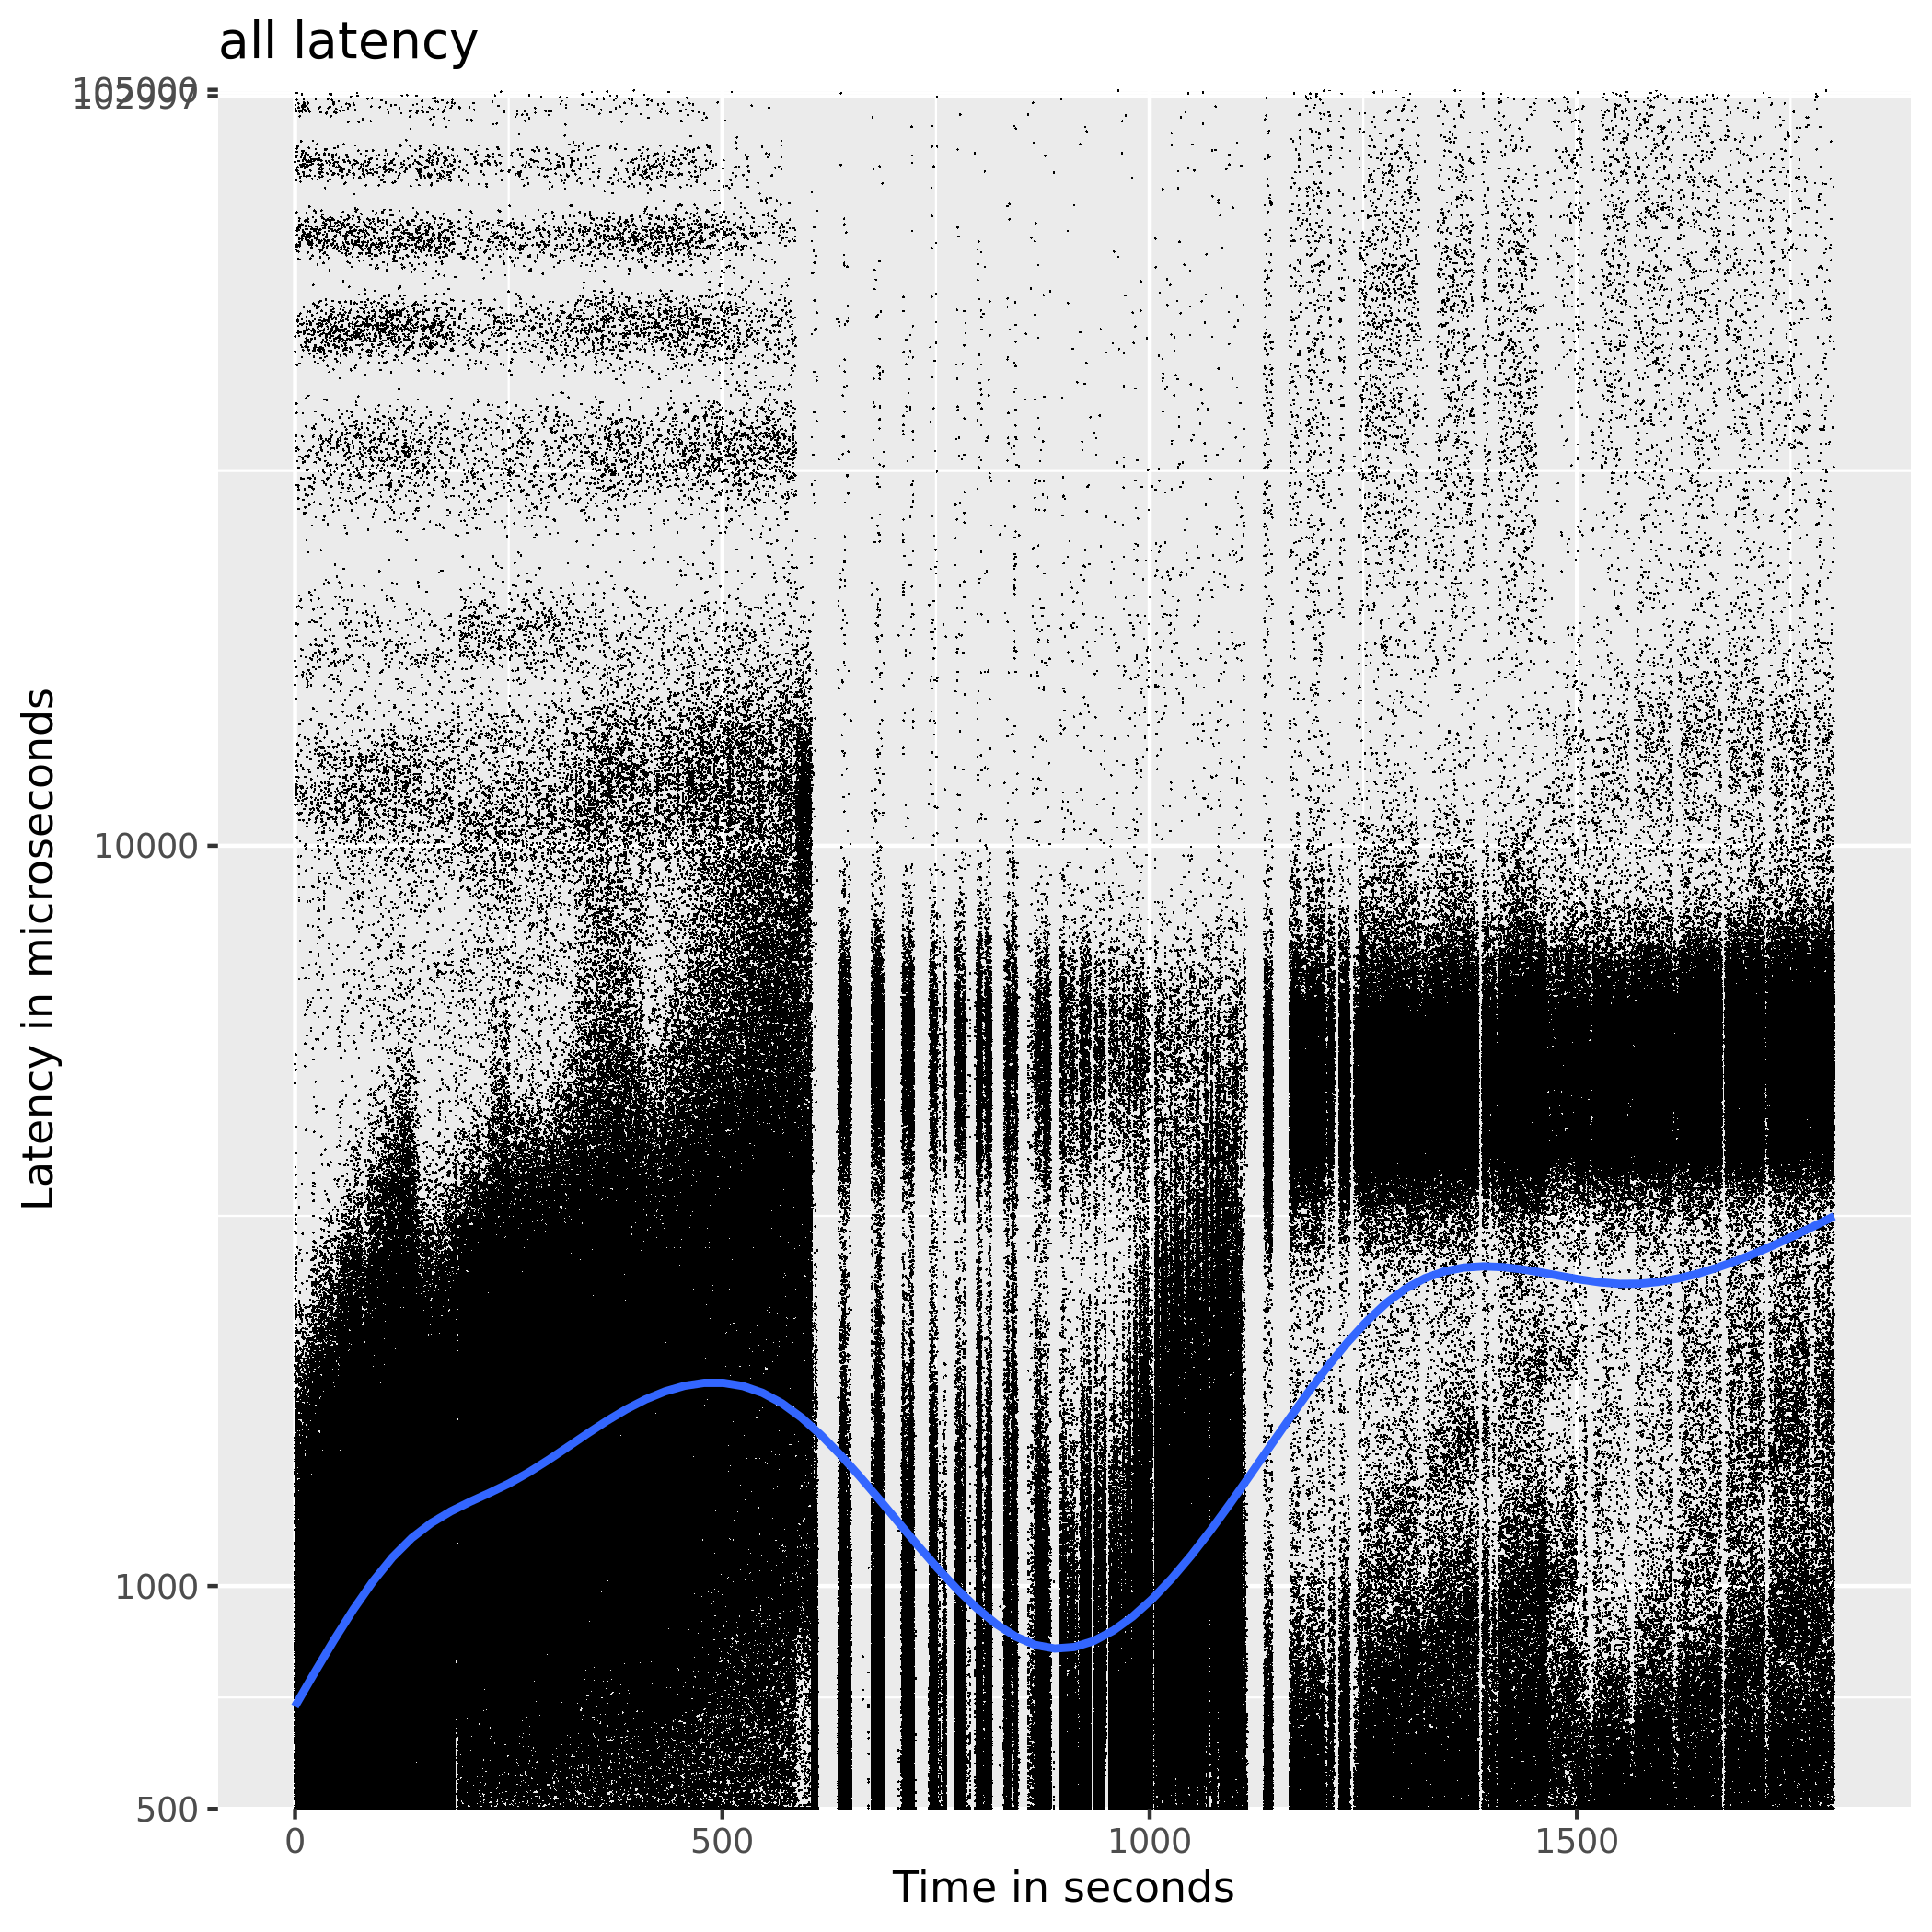
\includegraphics[width=0.5\textwidth]{RandomSlicing_Random_dynamic_write_heavy_latency}
\caption[\ac{RS} with Ramdom Replication Latency]{\ac{RS} with Ramdom Replication Latency. Comparison of the latency plots in the dynamic runs.}
\label{fig:random_slicing_random_dynamic_latency}
\end{figure}

Regarding the divergence from optimal load balance with \ac{RS} and Ring Jumping there is an absolute overall average divergence for key load of 0.022889616527552, for put load of 0.027008232485792, and for get load of 0.027078968645263.
Ignoring C0 with exactly three sections the highest divergence is measured in the dynamic configuration and the lowest is measured in C1.
This is quite intuitive as in C1 there are not many section and the sections are of a reasonable size while in the dynamic run the keys are potentially to the wrong node initially and will only be balanced after the repair operations are started for each key.

\subsection{Random Slicing Rotation}
The Ring Rotation \ac{RPS} implementation shows a lot of problems in the evaluation.
Apart from C0 and C1 every run with other configurations was far off any expected result or could not even be finished.
In C0 the throughput starts at about 3000 operations per second, steeply decreases to 1000 operations per second at 450s and from there slowly decreases to 500 operations per second.
In C1 the throughput starts at about 2100 operations per second, steeply decreases to 1000 operations per second at 500s and from there slowly decreases to 500 operations per second.
The first problematic run is the write-heavy run in C2, as the throughput stays at single-digit operations per second over the complete run, which can be seen in \cref{fig:random_slicing_rotation_throughput}.
\begin{figure}
\center
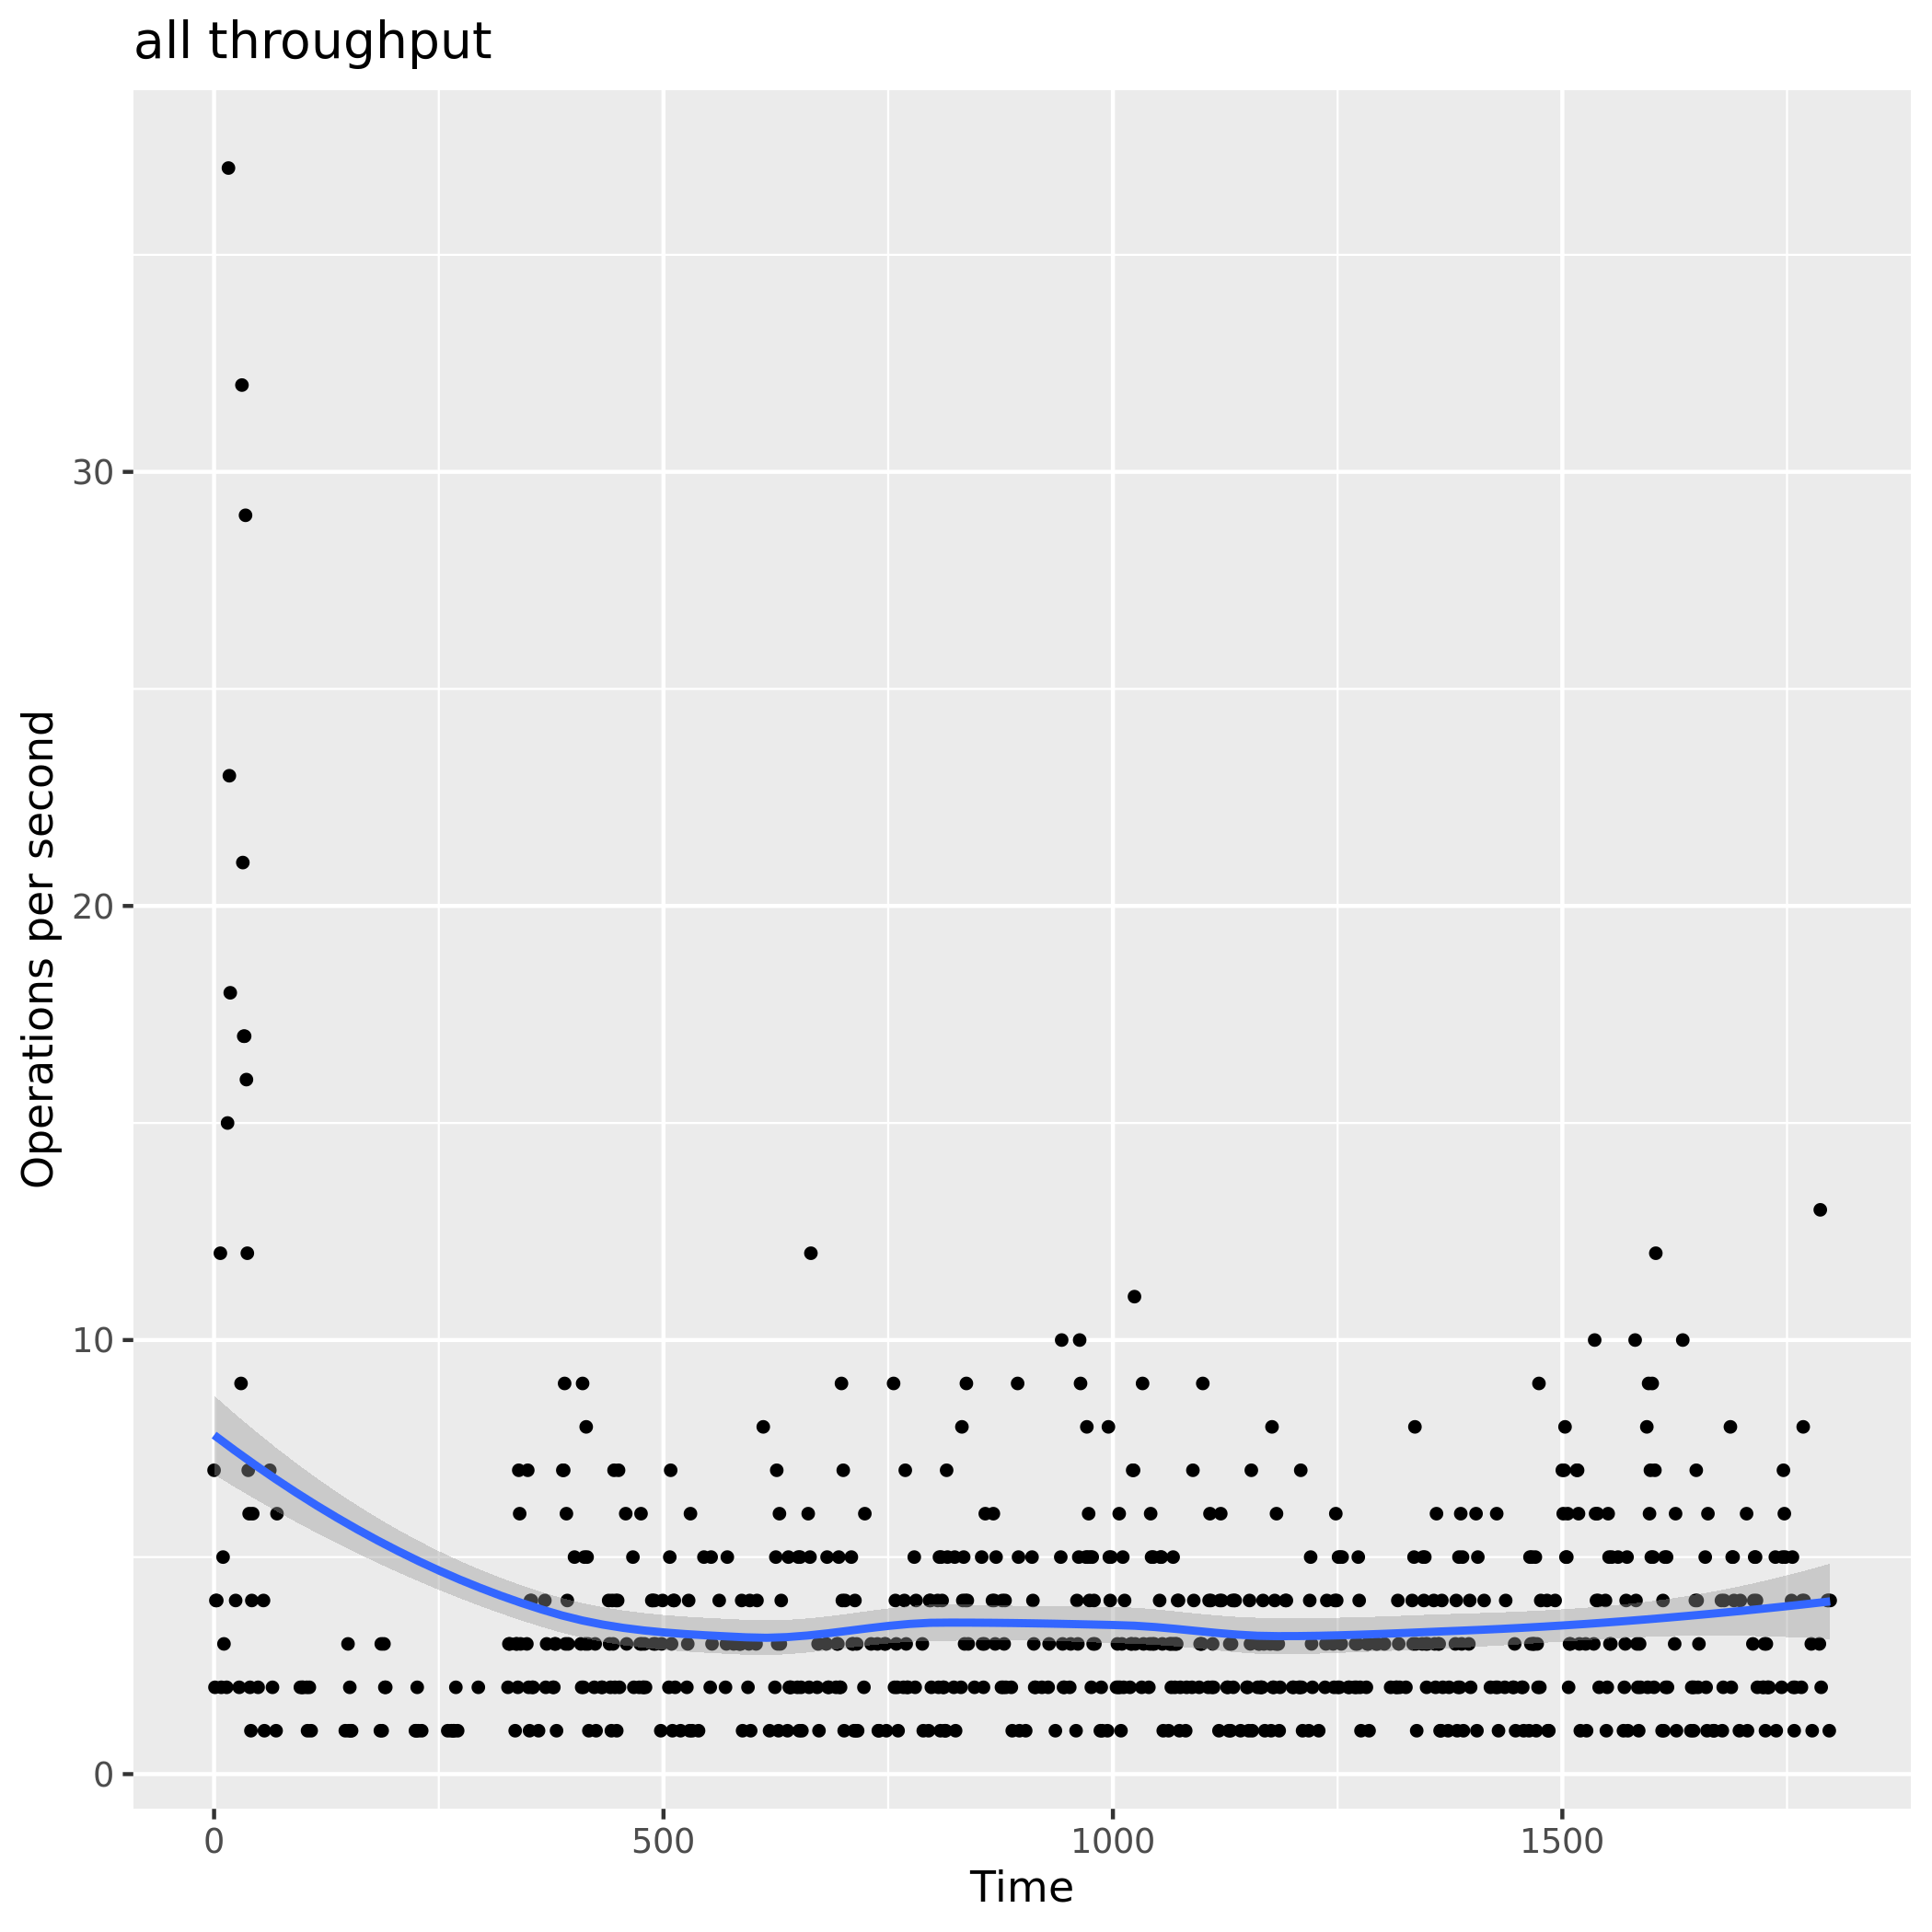
\includegraphics[width=0.5\textwidth]{RandomSlicing_Rotation_C2_write_heavy_throughput}
\caption[Low Throughput with Ring Rotation]{Low Throughput with Ring Rotation}
\label{fig:random_slicing_rotation_throughput}
\end{figure}
Trying to rerun this configuration to confirm the result showed a potential memory leak that seems to be occur more frequently with a higher number of sections.

This memory leak became quite apparent as even after multiple restarts the benchmark runs could not be finished in the dynamic configurations as the memory leak caused the run to crash each time.
An assertion on the overall load balance is also impossible through this.


\subsection{Comparison}
In this section we compare the evaluation results of the different \ac{RCL} configurations and focus on how our hypotheses are supported or contradicted.
As there is not enough data and configurations to properly test the hypotheses we use the available evaluation data to quantitatively compare the different approaches.

\subsubsection{Hypothesis 1}
Hypothesis 1 claims that \ac{RS} has the best load balance when Random Replication is used as the replication placement strategy.
As Random Replication produces the better overall load balance and also has a lower absolute divergence for every configuration and parameter than Ring Rotation and Ring Jumping we can assume Hypothesis 1 as plausible.

\subsubsection{Hypothesis 2}
Hypothesis 2 claims that \ac{RS} has the highest throughput when Random Replication is used as the replication placement strategy.
Apart from the Ring Rotation strategy, which shows a strong decline in throughput with a growing number of ring sections, the throughput plots have the same characteristics for the different \acp{RPS}.
They show that the throughput starts at about the same rate, decreases to similar values at equal times and also ends at the same rate.
Therefore there is no argument for or against the hypothesis with the available data and as is shown with Ring Rotation it may be a matter of scalability of the strategies.

\subsubsection{Hypothesis 3}
Hypothesis 3 claims that the load divergence of \ac{RS} with the best replication placement strategy is at most 10\% higher than with Consistent Hashing.
We use the results of \ac{RS} with Random Replication as this yielded the best balancing properties and a high throughput.
While the divergence of load concerning unique keys with \ac{RS} is nearly 6 times the one with Consistent Hashing, the divergence concerning operations is only slightly more than 10\% higher.
However, this clearly shows strong arguments against the presented hypothesis for the current integration of \ac{RS} with \ac{RCL}.
As a side remark it is interesting to see that \ac{RS} with Consistent Hashing achieves a way better load balance in configuration C2 than Consistent Hashing and it will be interesting to see how both systems scale for more nodes.

\subsubsection{Hypothesis 4}
Hypothesis 4 claims that \ac{RS} generates a throughput that is nearly as good as Consistent Hashing in a static cluster configuration.
As there is no clear difference in throughput we choose Random Replication as the replication placement strategy.
As can be seen in the side-to-side comparison in \cref{fig:throughput_comparison} there is no significant difference between Consistent Hashing and \ac{RS} in any static configuration.
\begin{figure}
\begin{subfigure}{0.5\textwidth}
	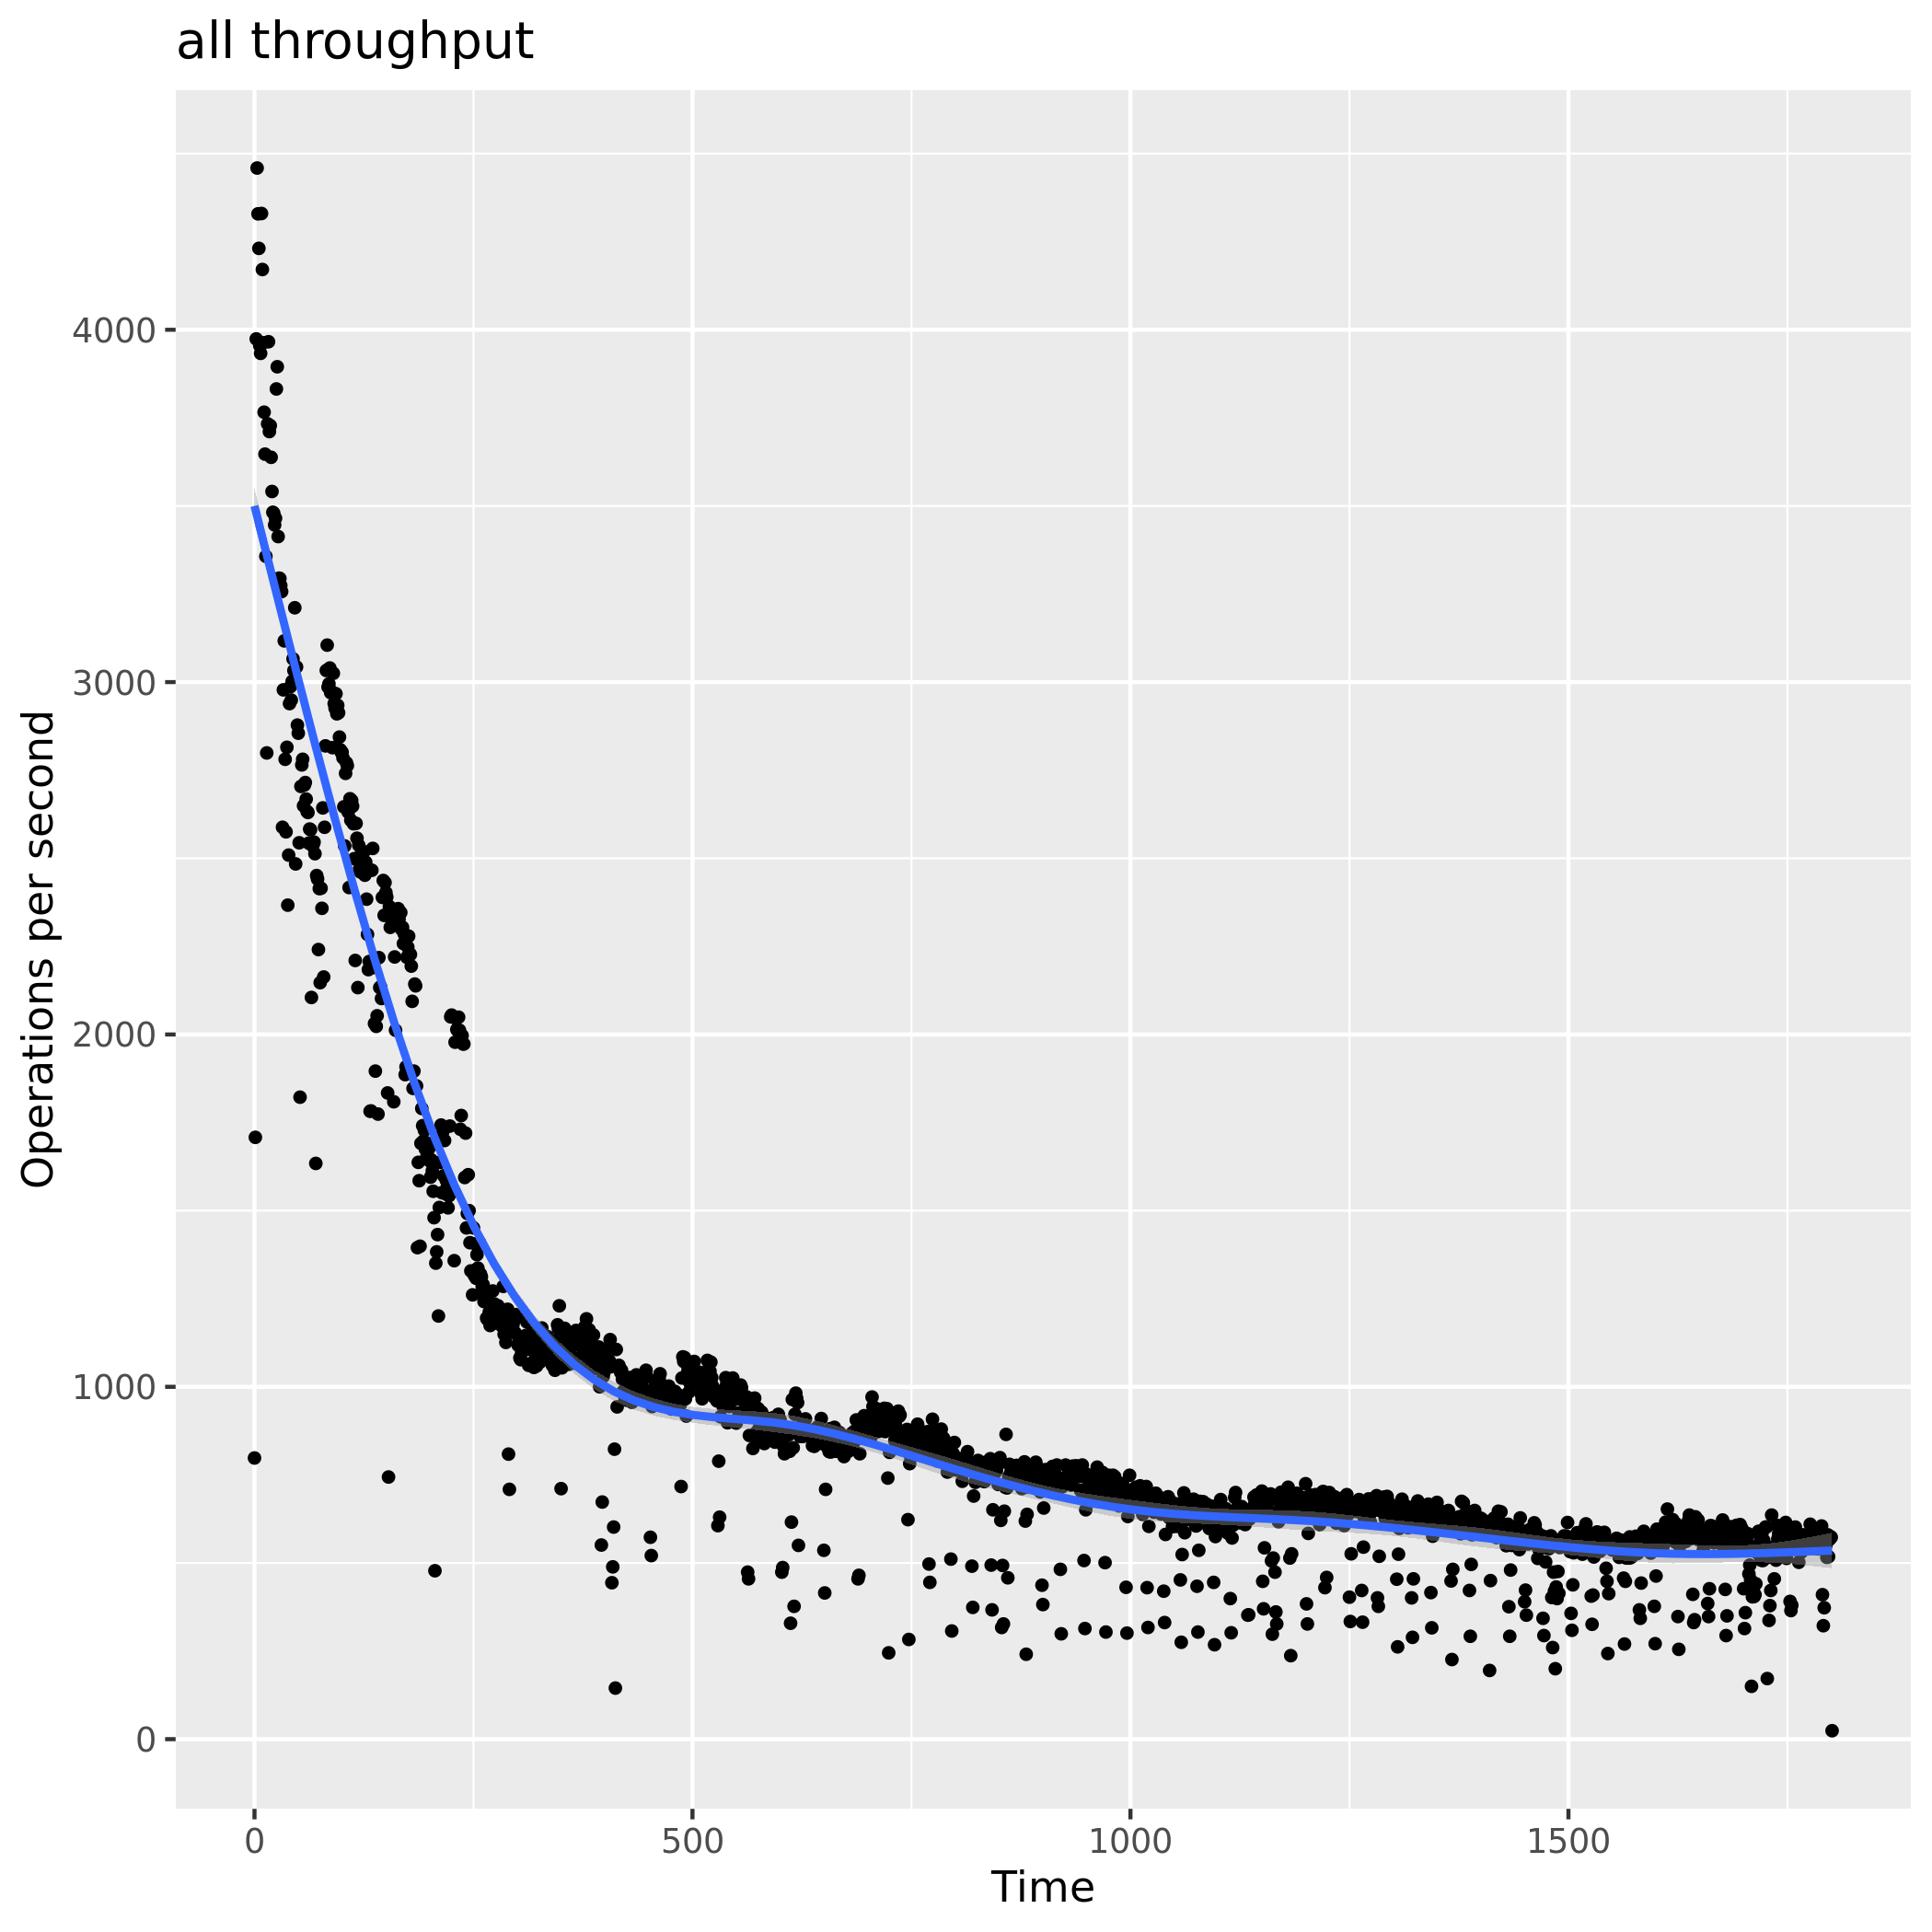
\includegraphics[width=0.8\textwidth]{ConsistentHashing_C0_write_heavy_throughput}
	\caption[Throughput for Consistent Hashing in C0]{Throughput for Consistent Hashing in C0}
\end{subfigure}
\begin{subfigure}{0.5\textwidth}
	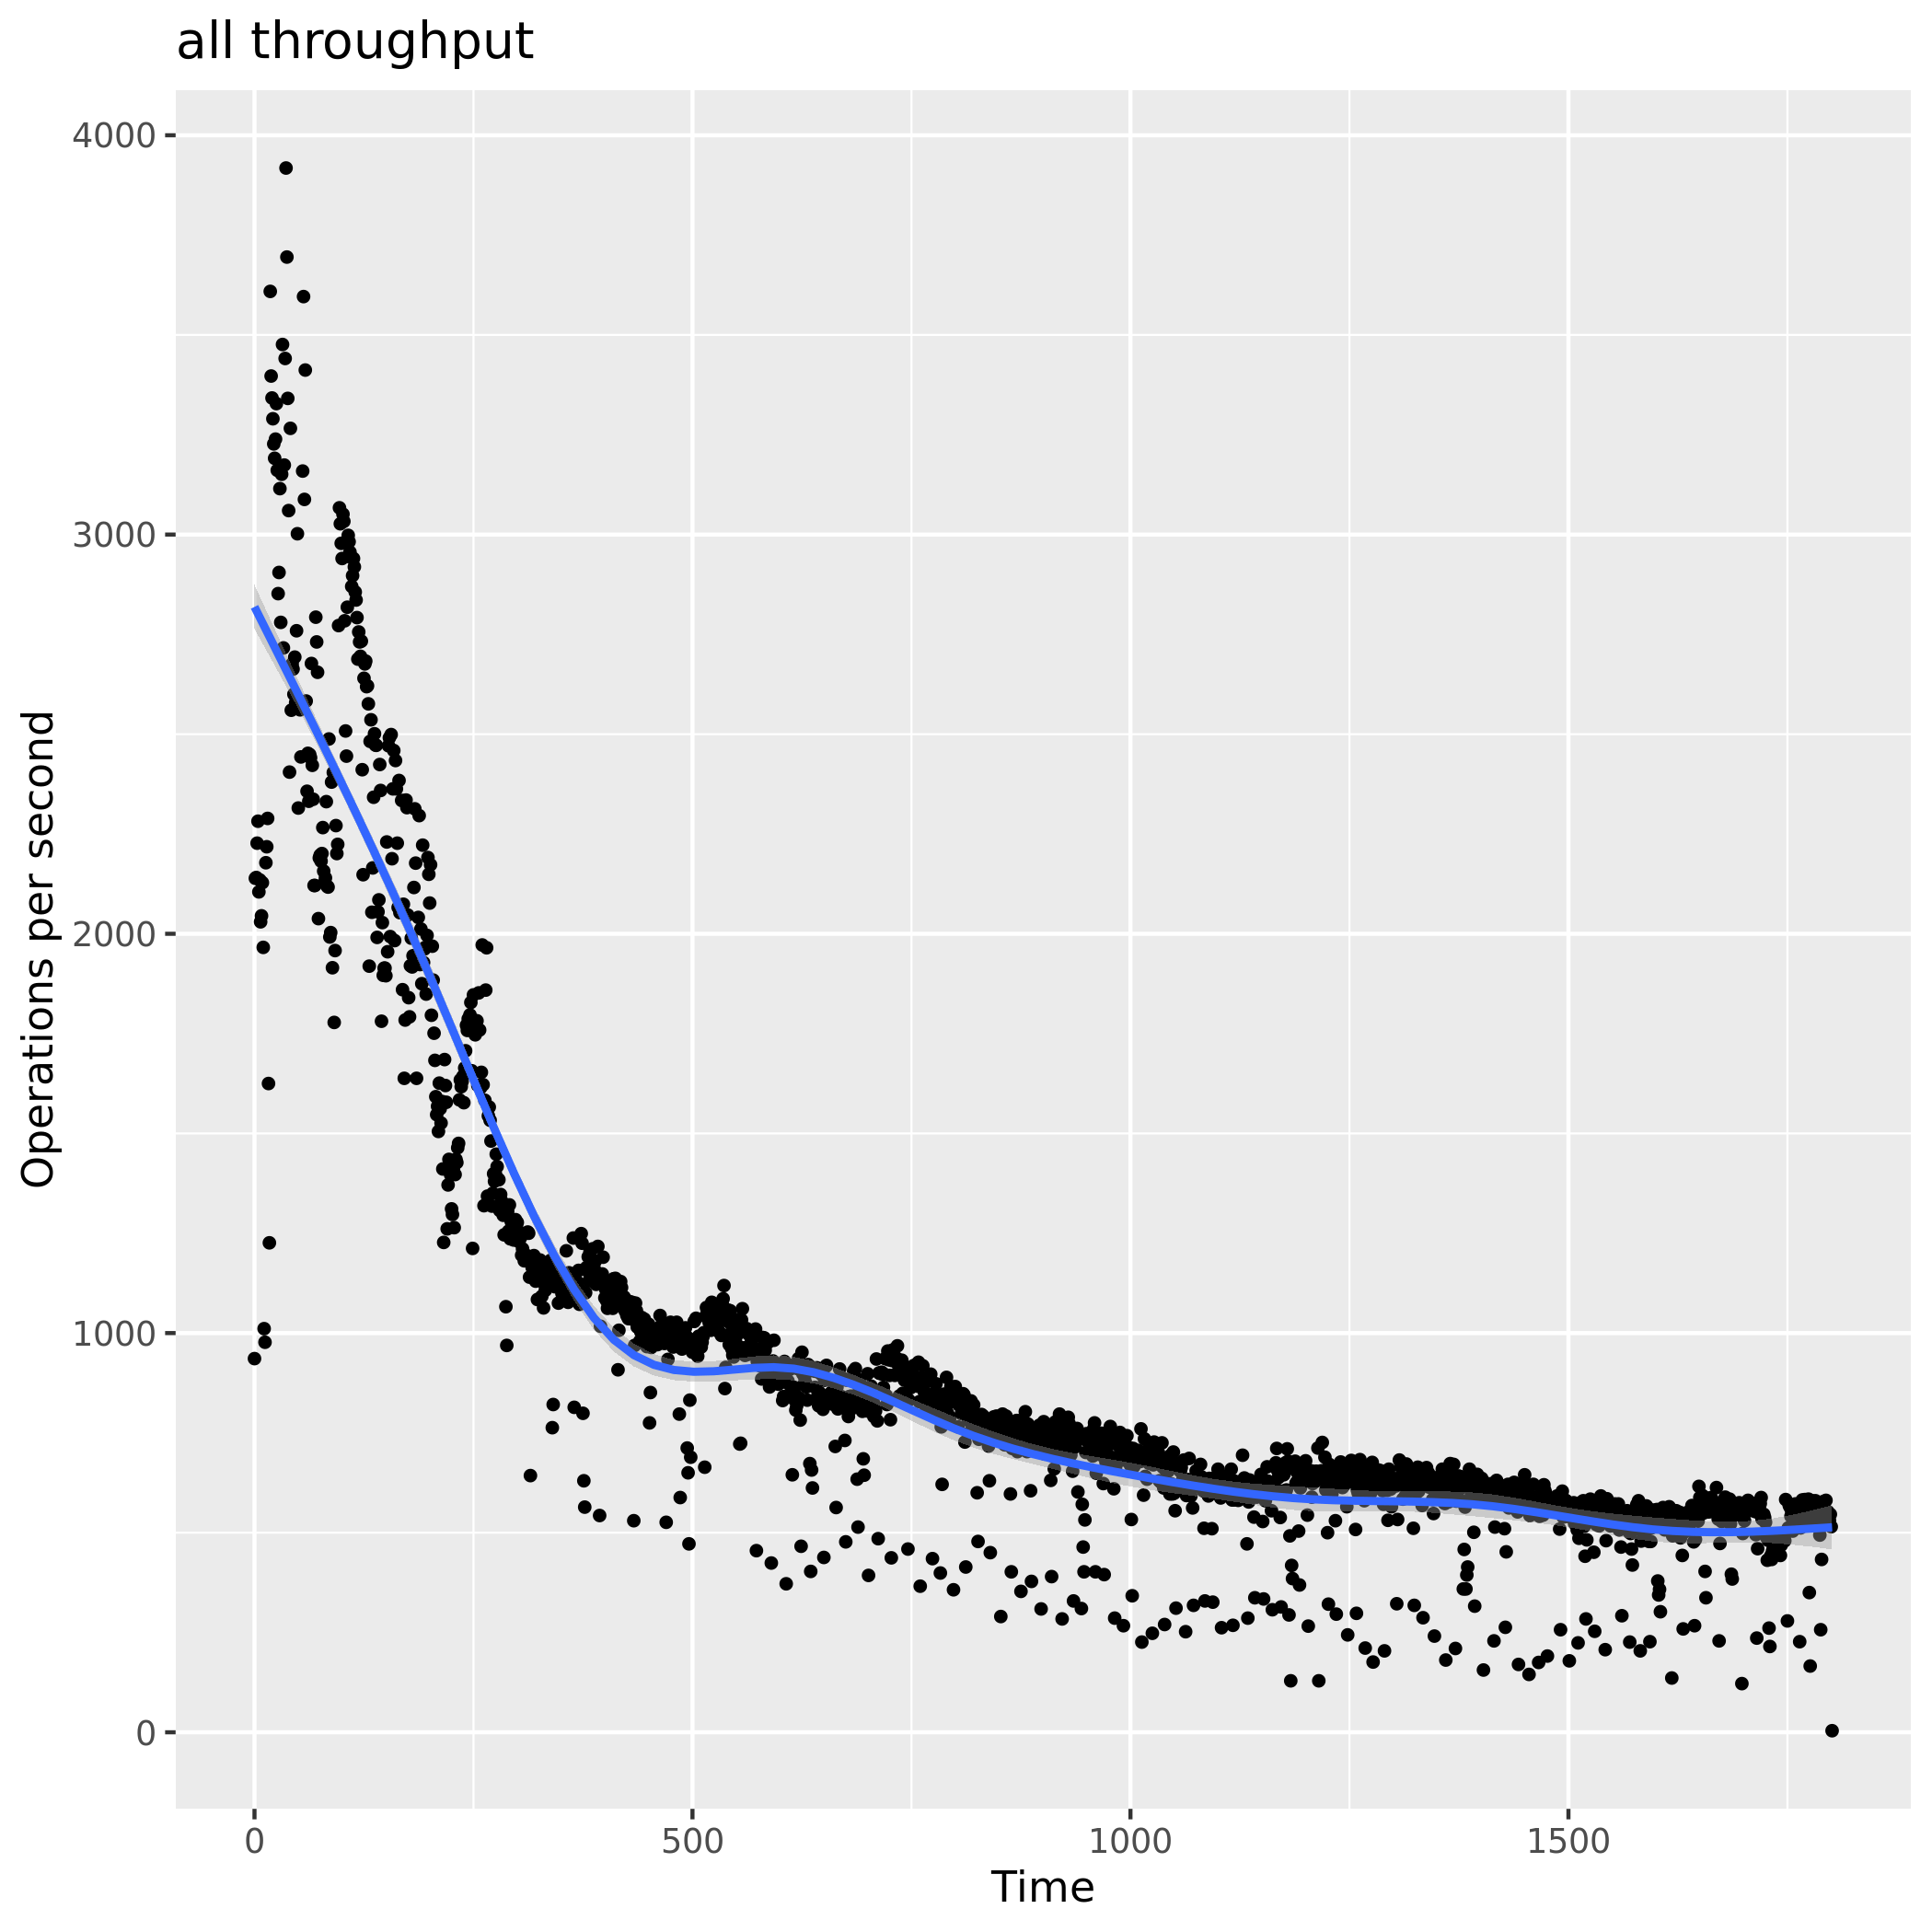
\includegraphics[width=0.8\textwidth]{RandomSlicing_Random_C0_write_heavy_throughput}
	\caption[Throughput for \ac{RS} in C0]{Throughput for \ac{RS} in C0}
\end{subfigure}
\begin{subfigure}{0.5\textwidth}
	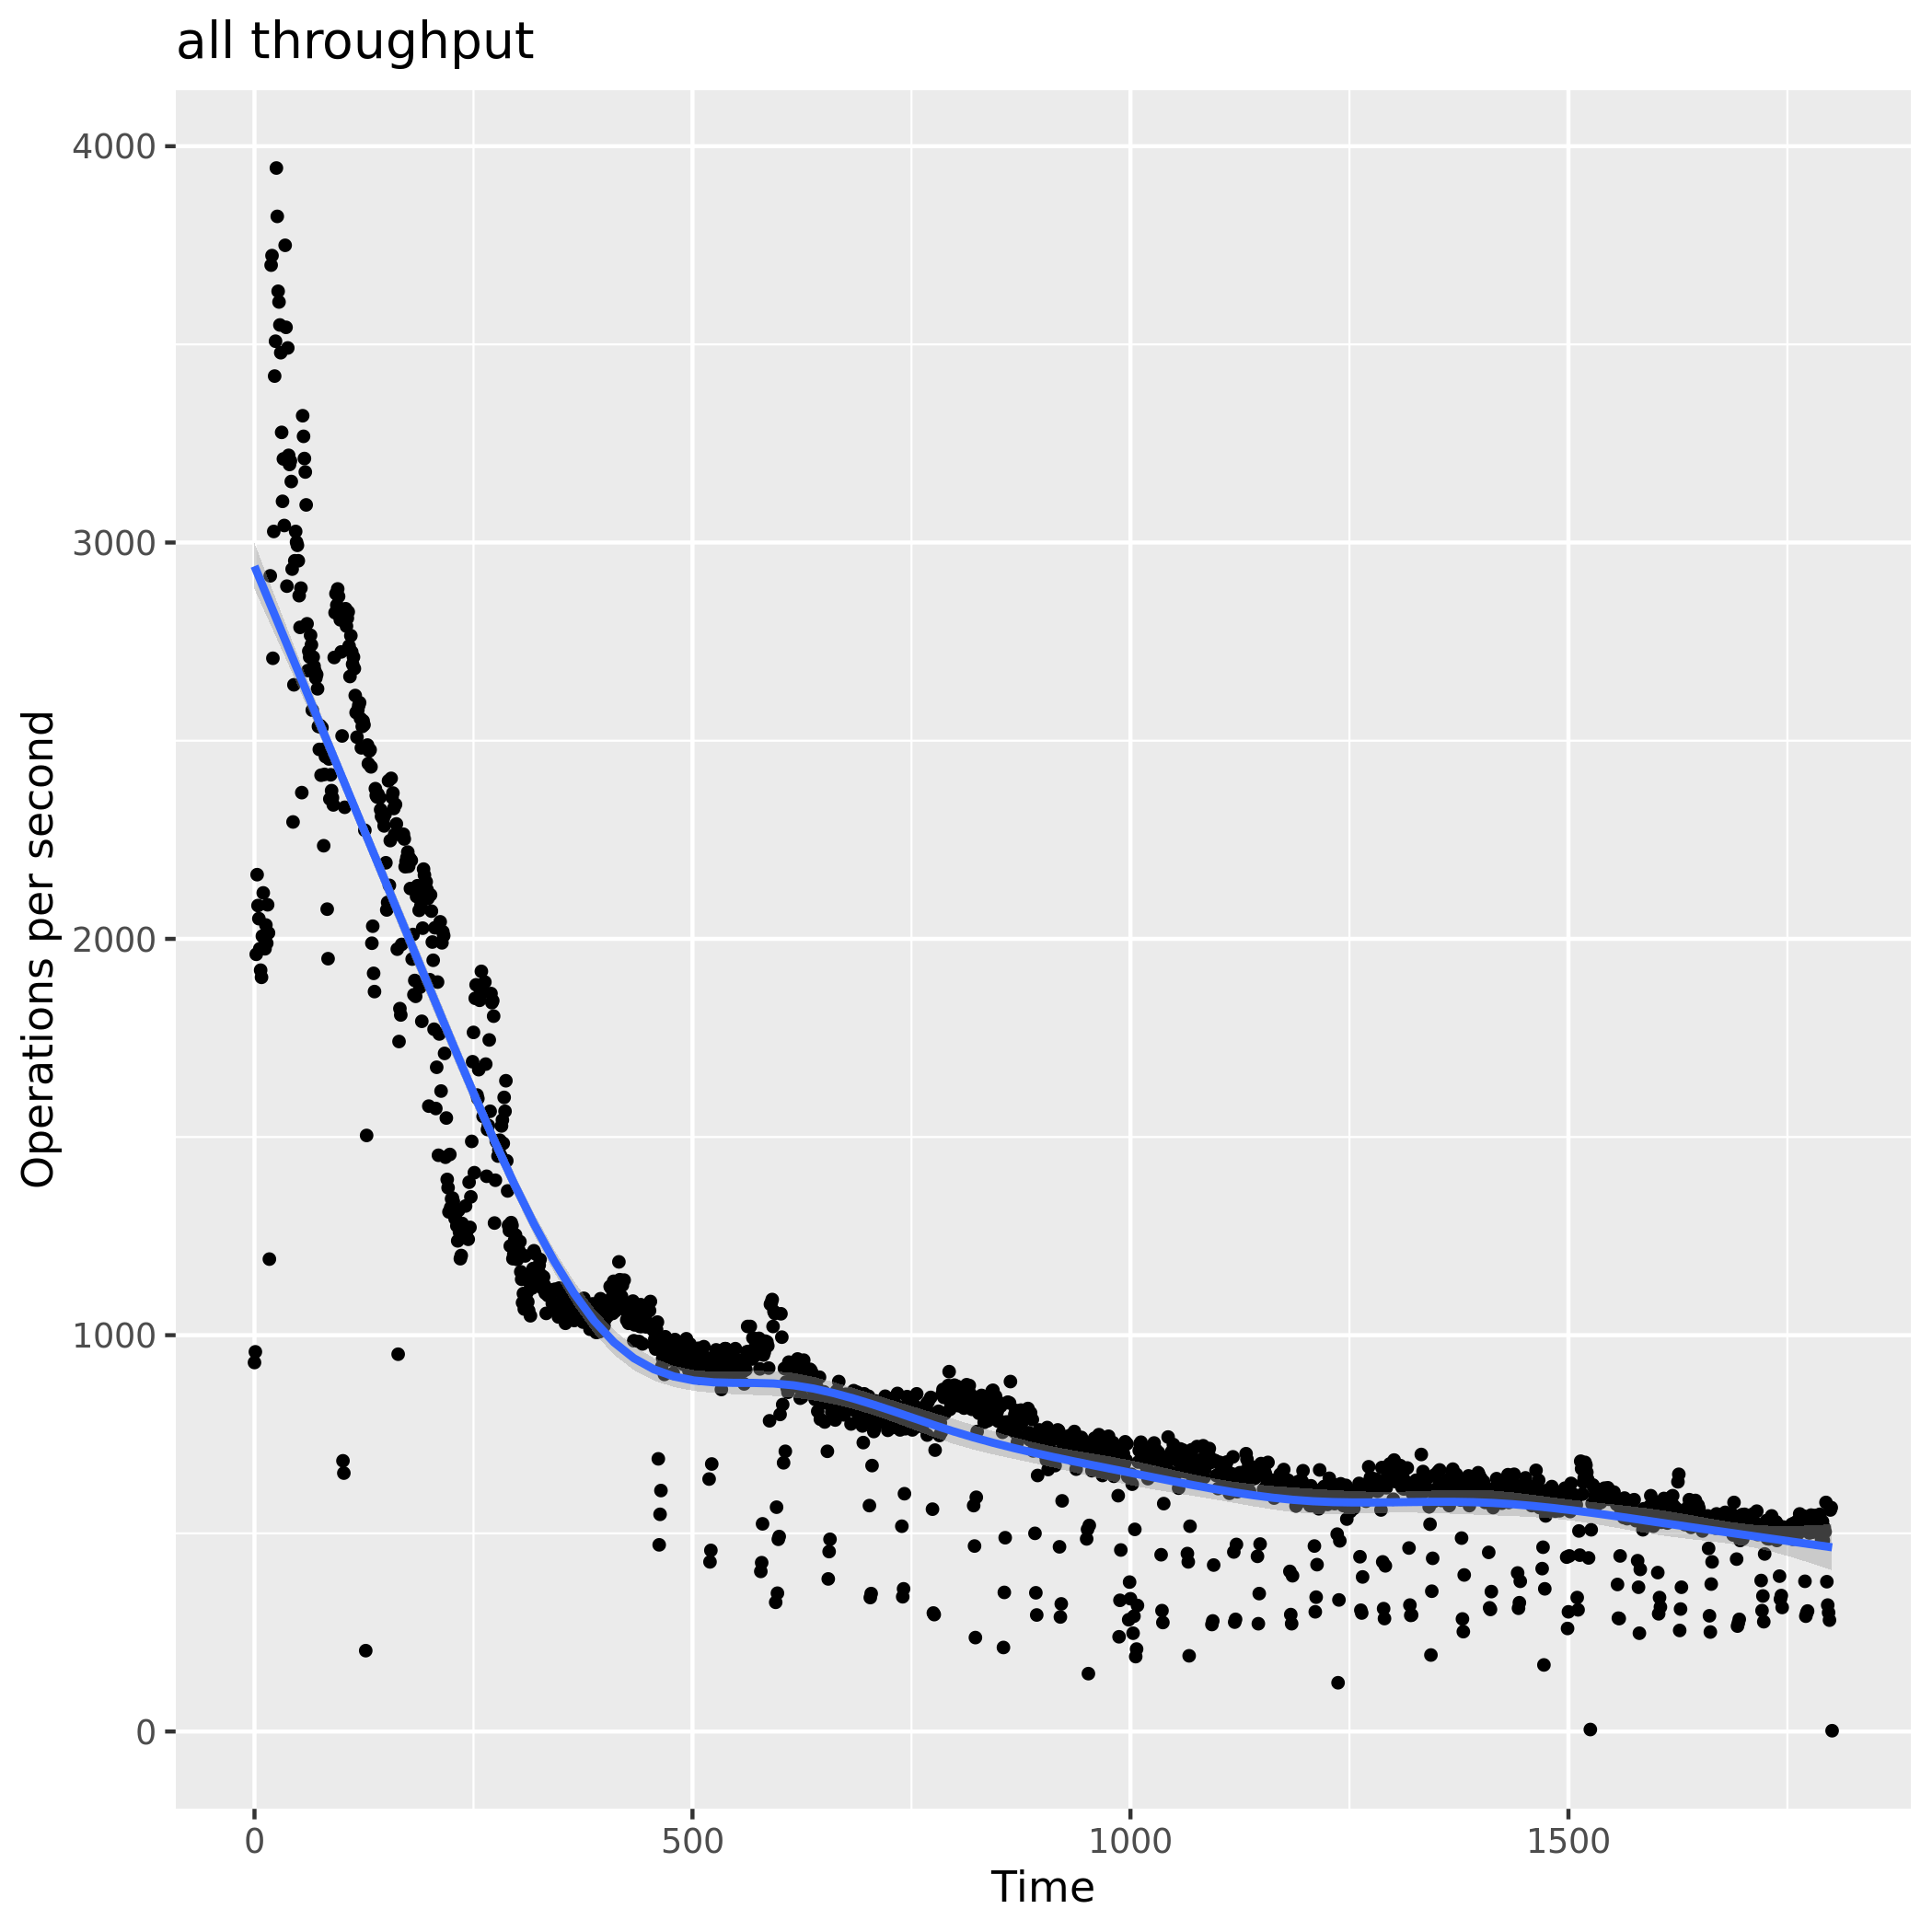
\includegraphics[width=0.8\textwidth]{ConsistentHashing_C1_read_heavy_throughput}
	\caption[Throughput for Consistent Hashing in C1]{Throughput for Consistent Hashing in C1}
\end{subfigure}
\begin{subfigure}{0.5\textwidth}
	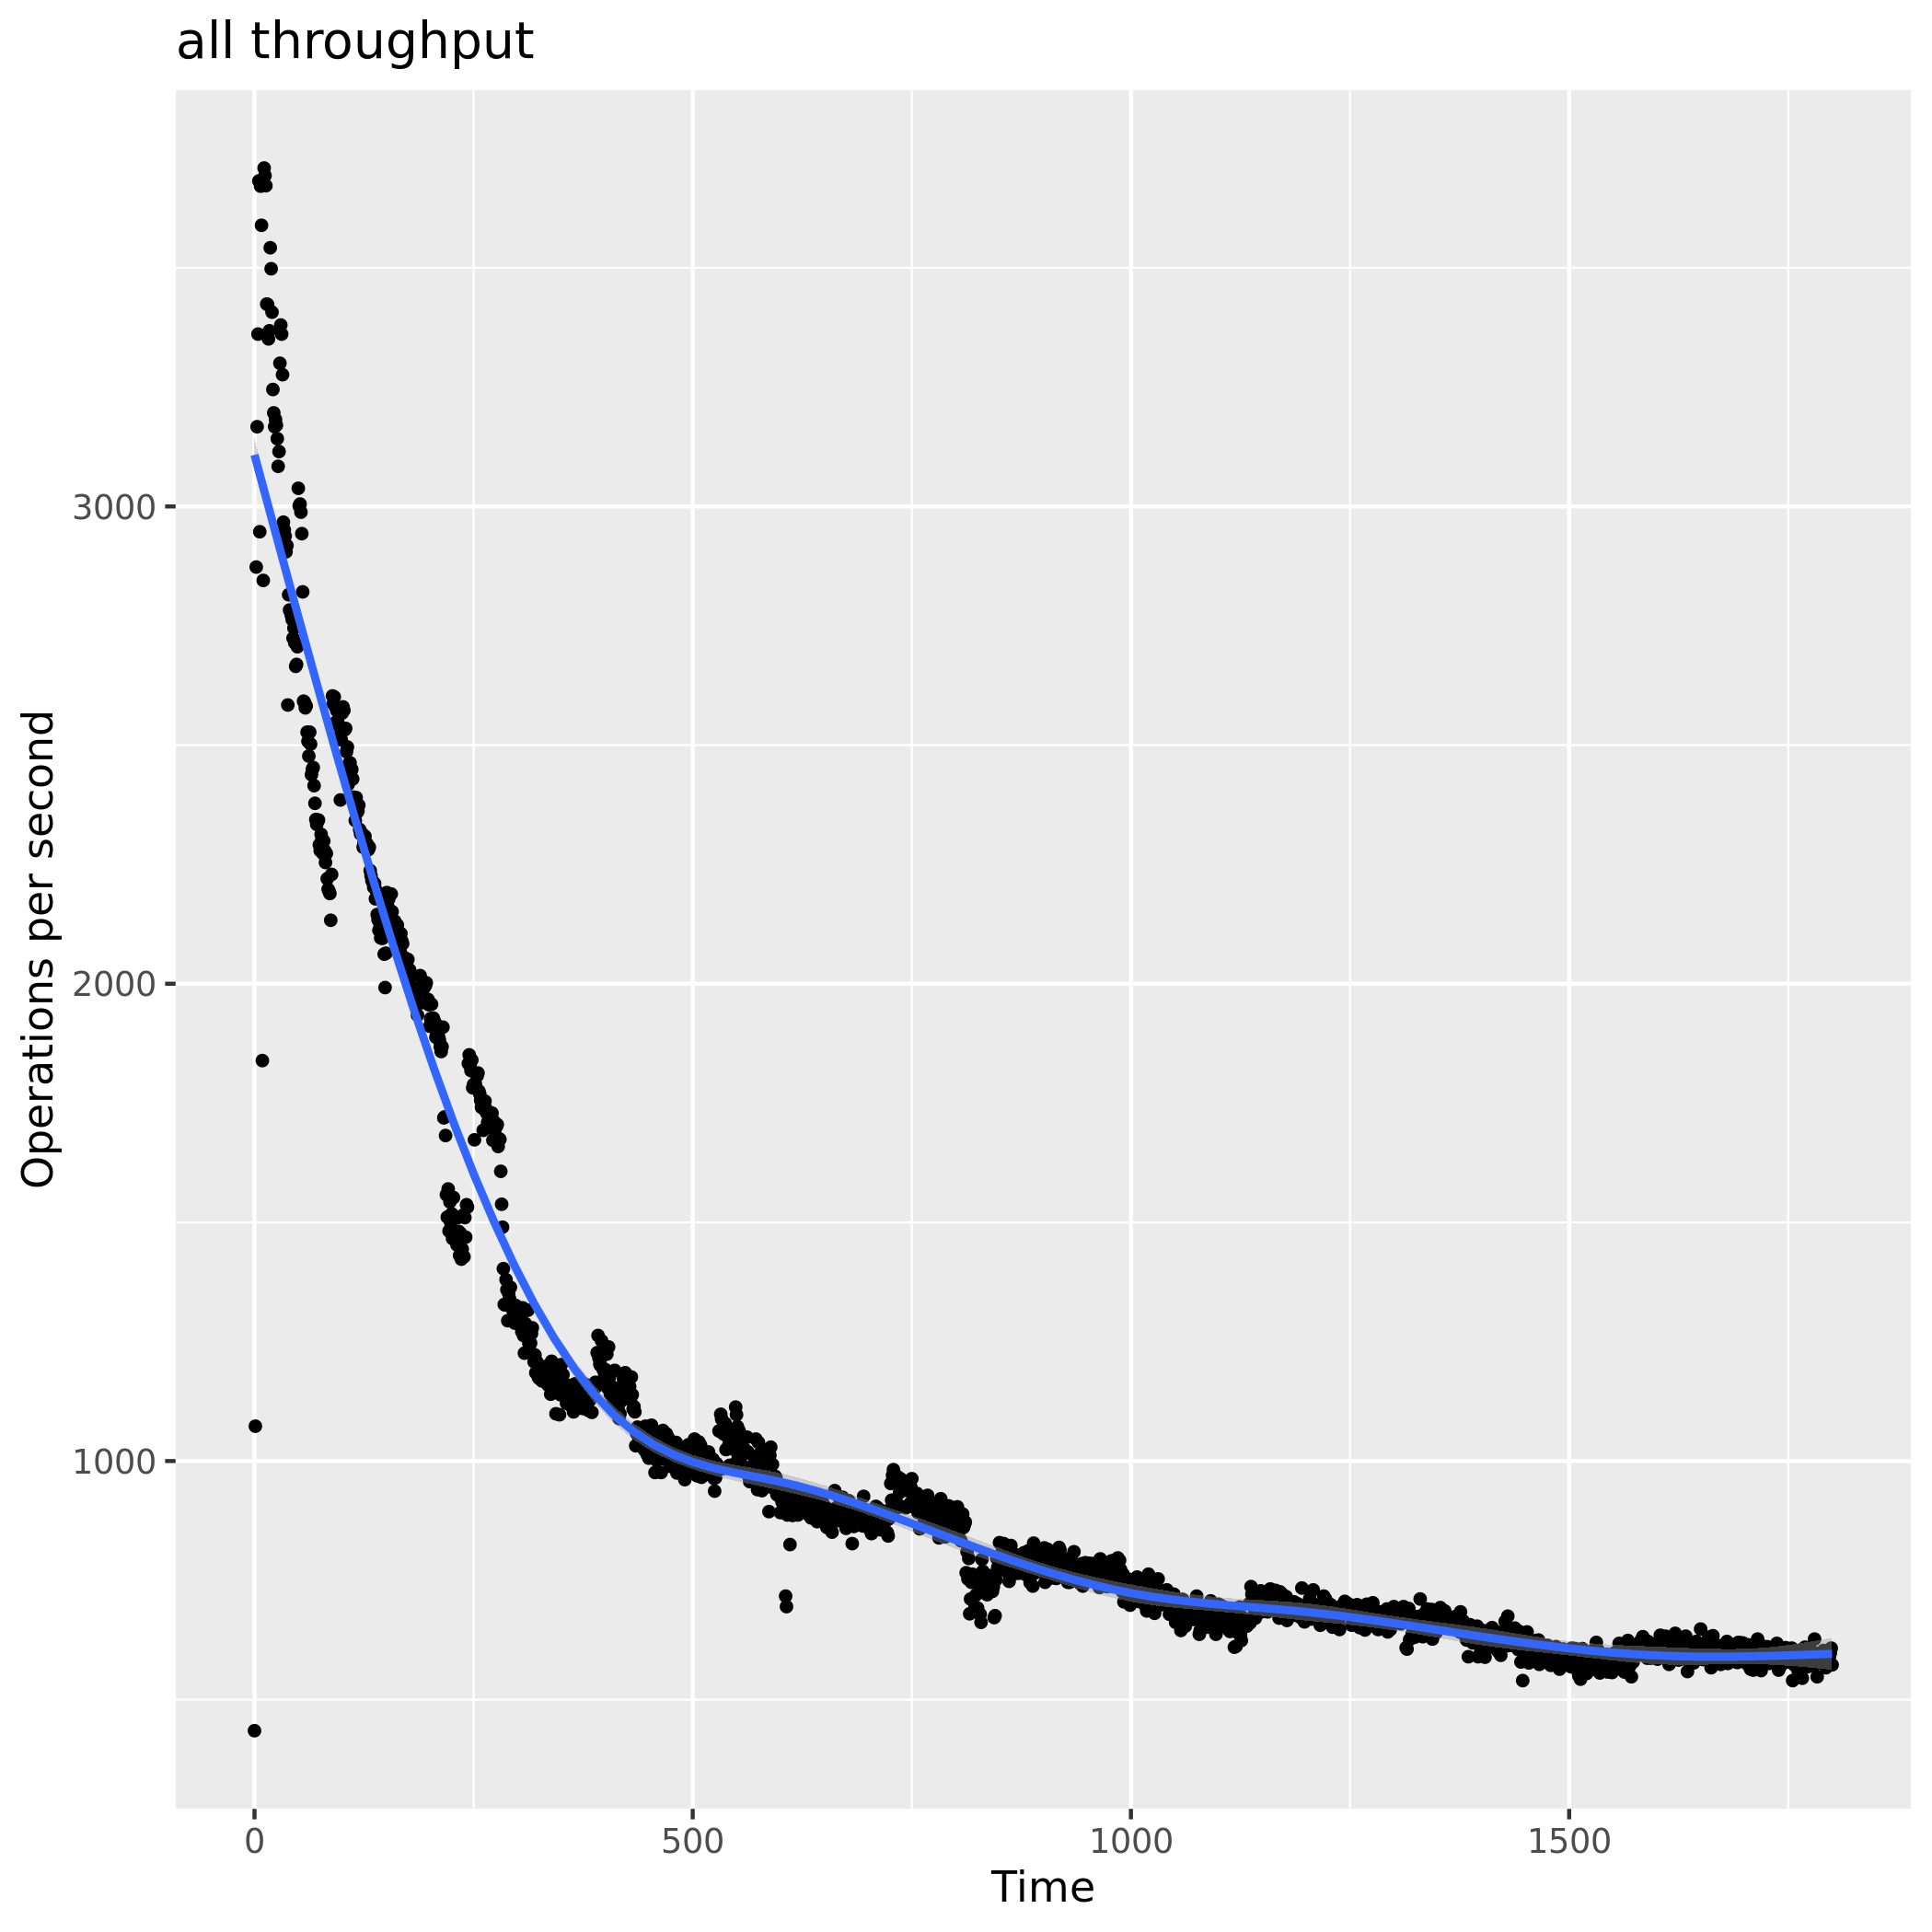
\includegraphics[width=0.8\textwidth]{RandomSlicing_Random_C1_read_heavy_throughput}
	\caption[Throughput for \ac{RS} in C1]{Throughput for \ac{RS} in C1}
\end{subfigure}
\begin{subfigure}{0.5\textwidth}
	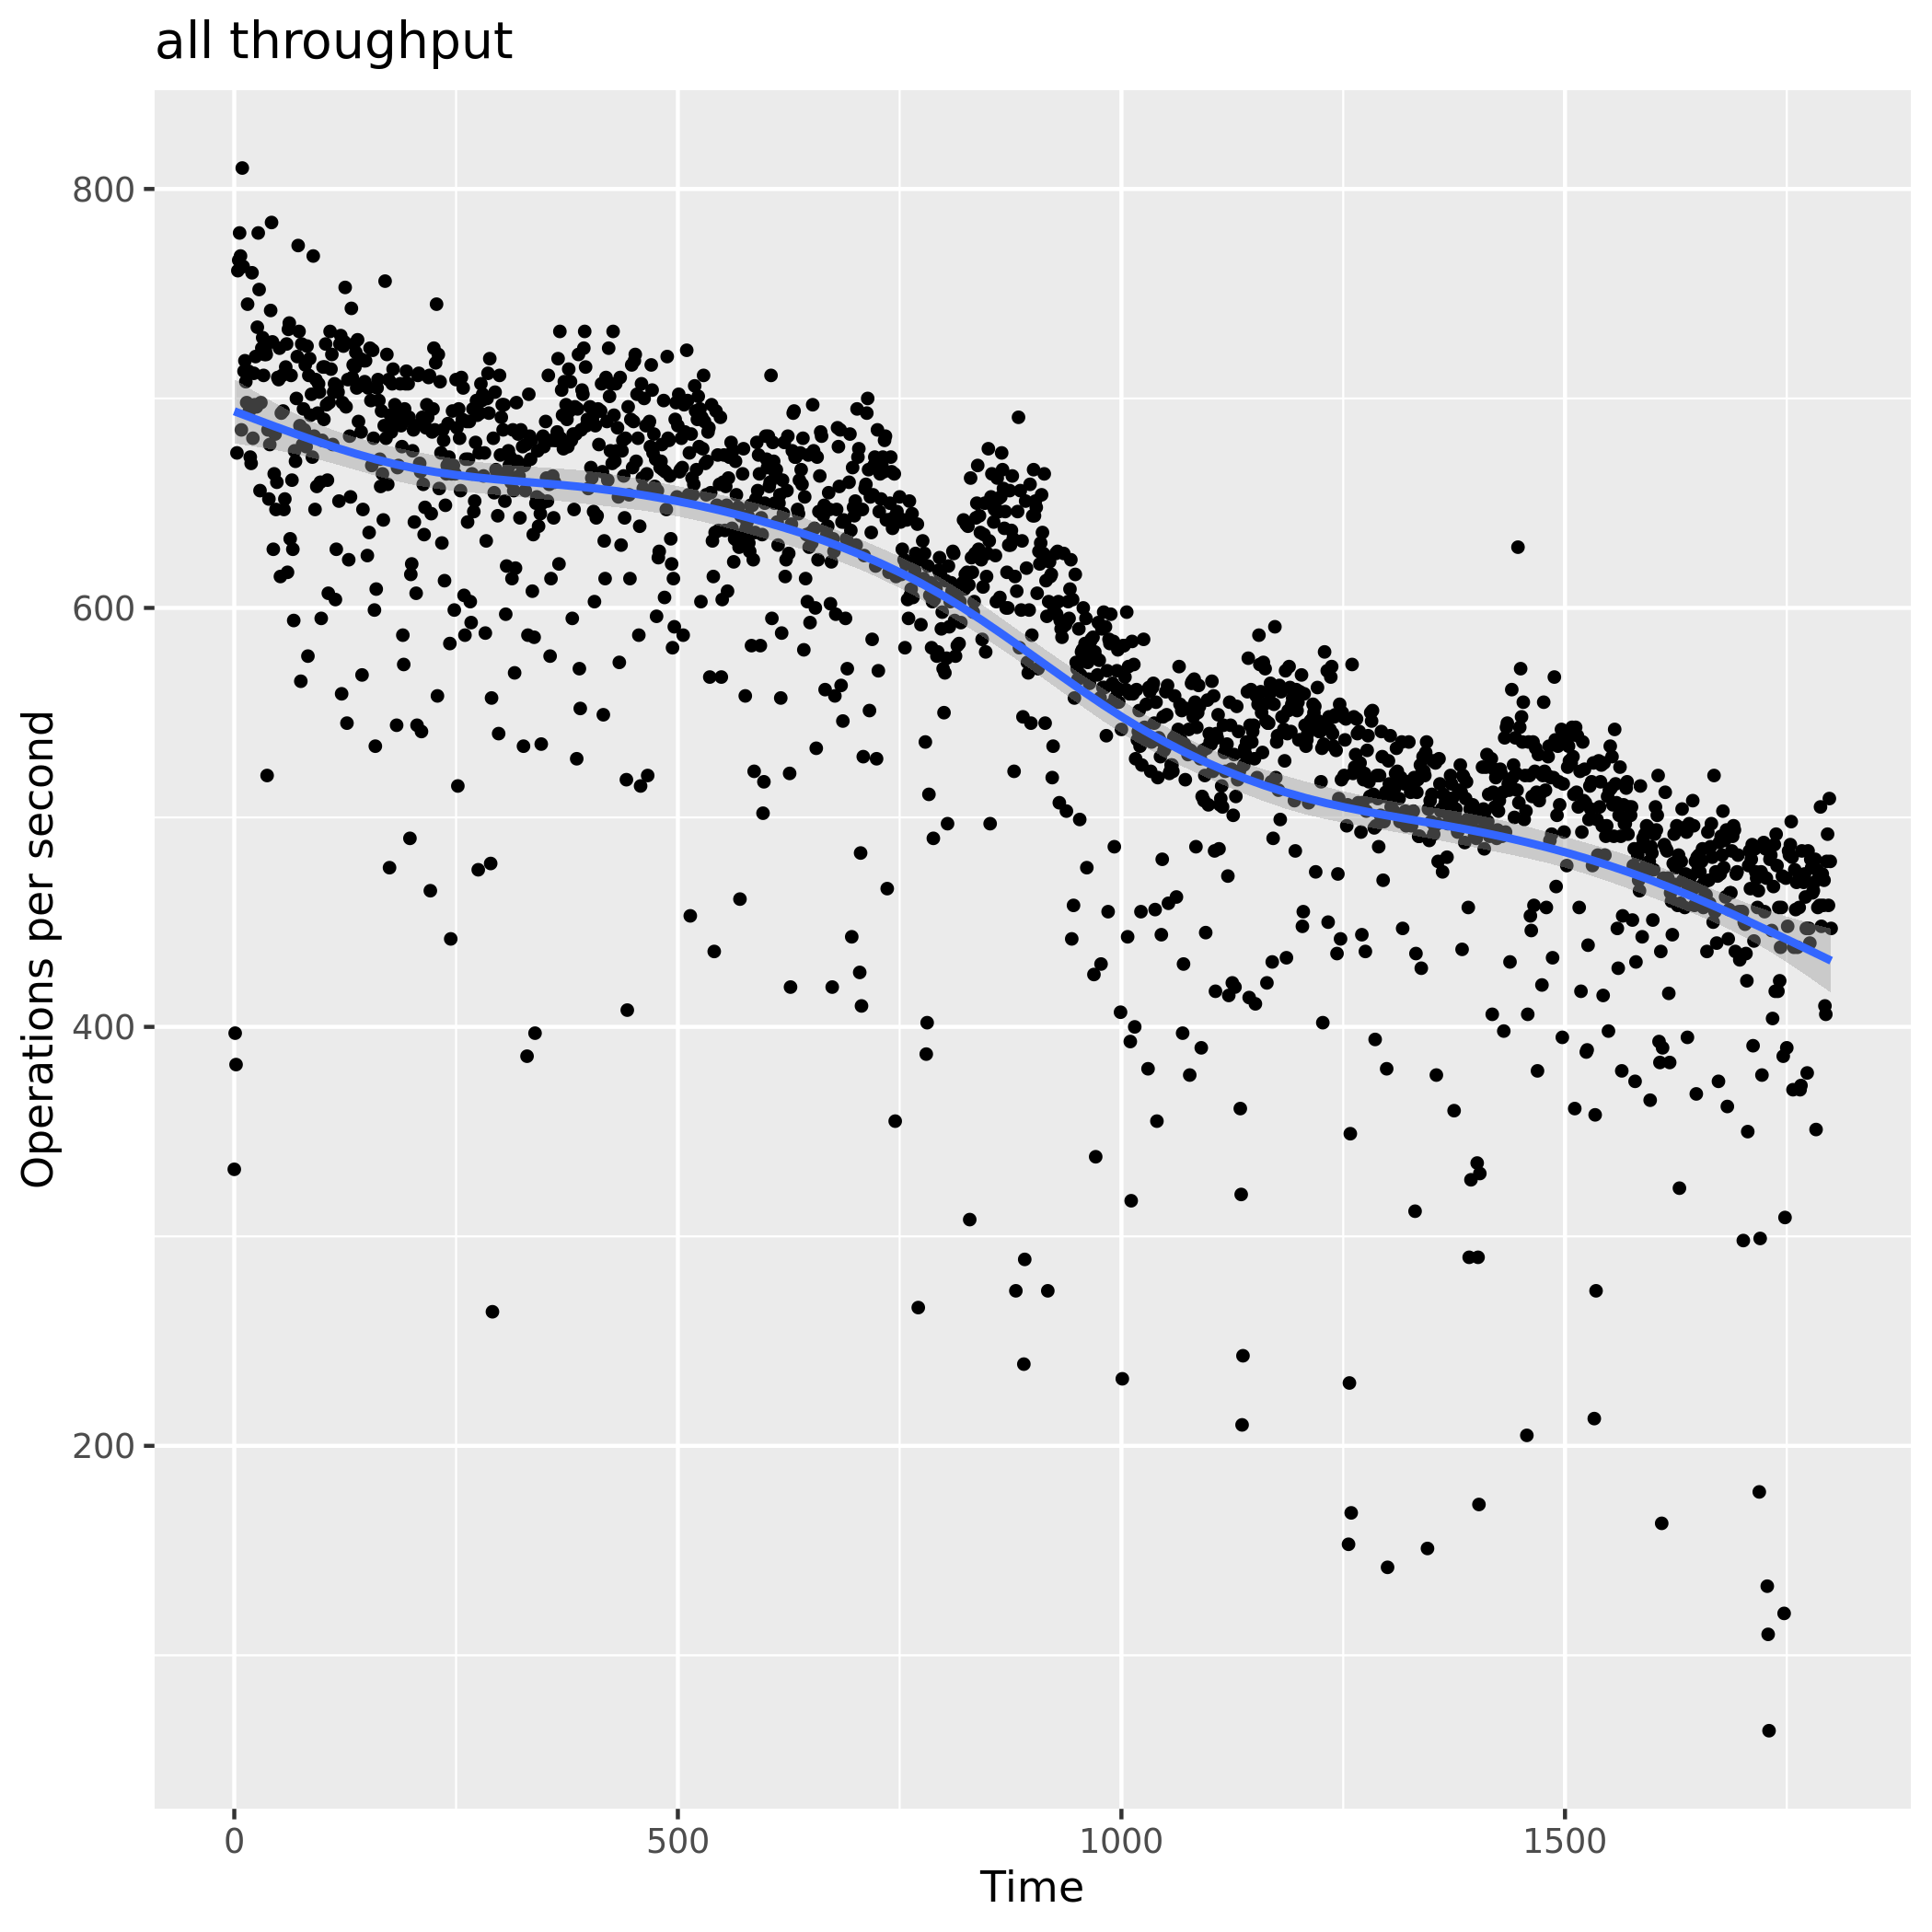
\includegraphics[width=0.8\textwidth]{ConsistentHashing_C2_write_heavy_throughput}
	\caption[Throughput for Consistent Hashing in C2]{Throughput for Consistent Hashing in C2}
\end{subfigure}
\begin{subfigure}{0.5\textwidth}
	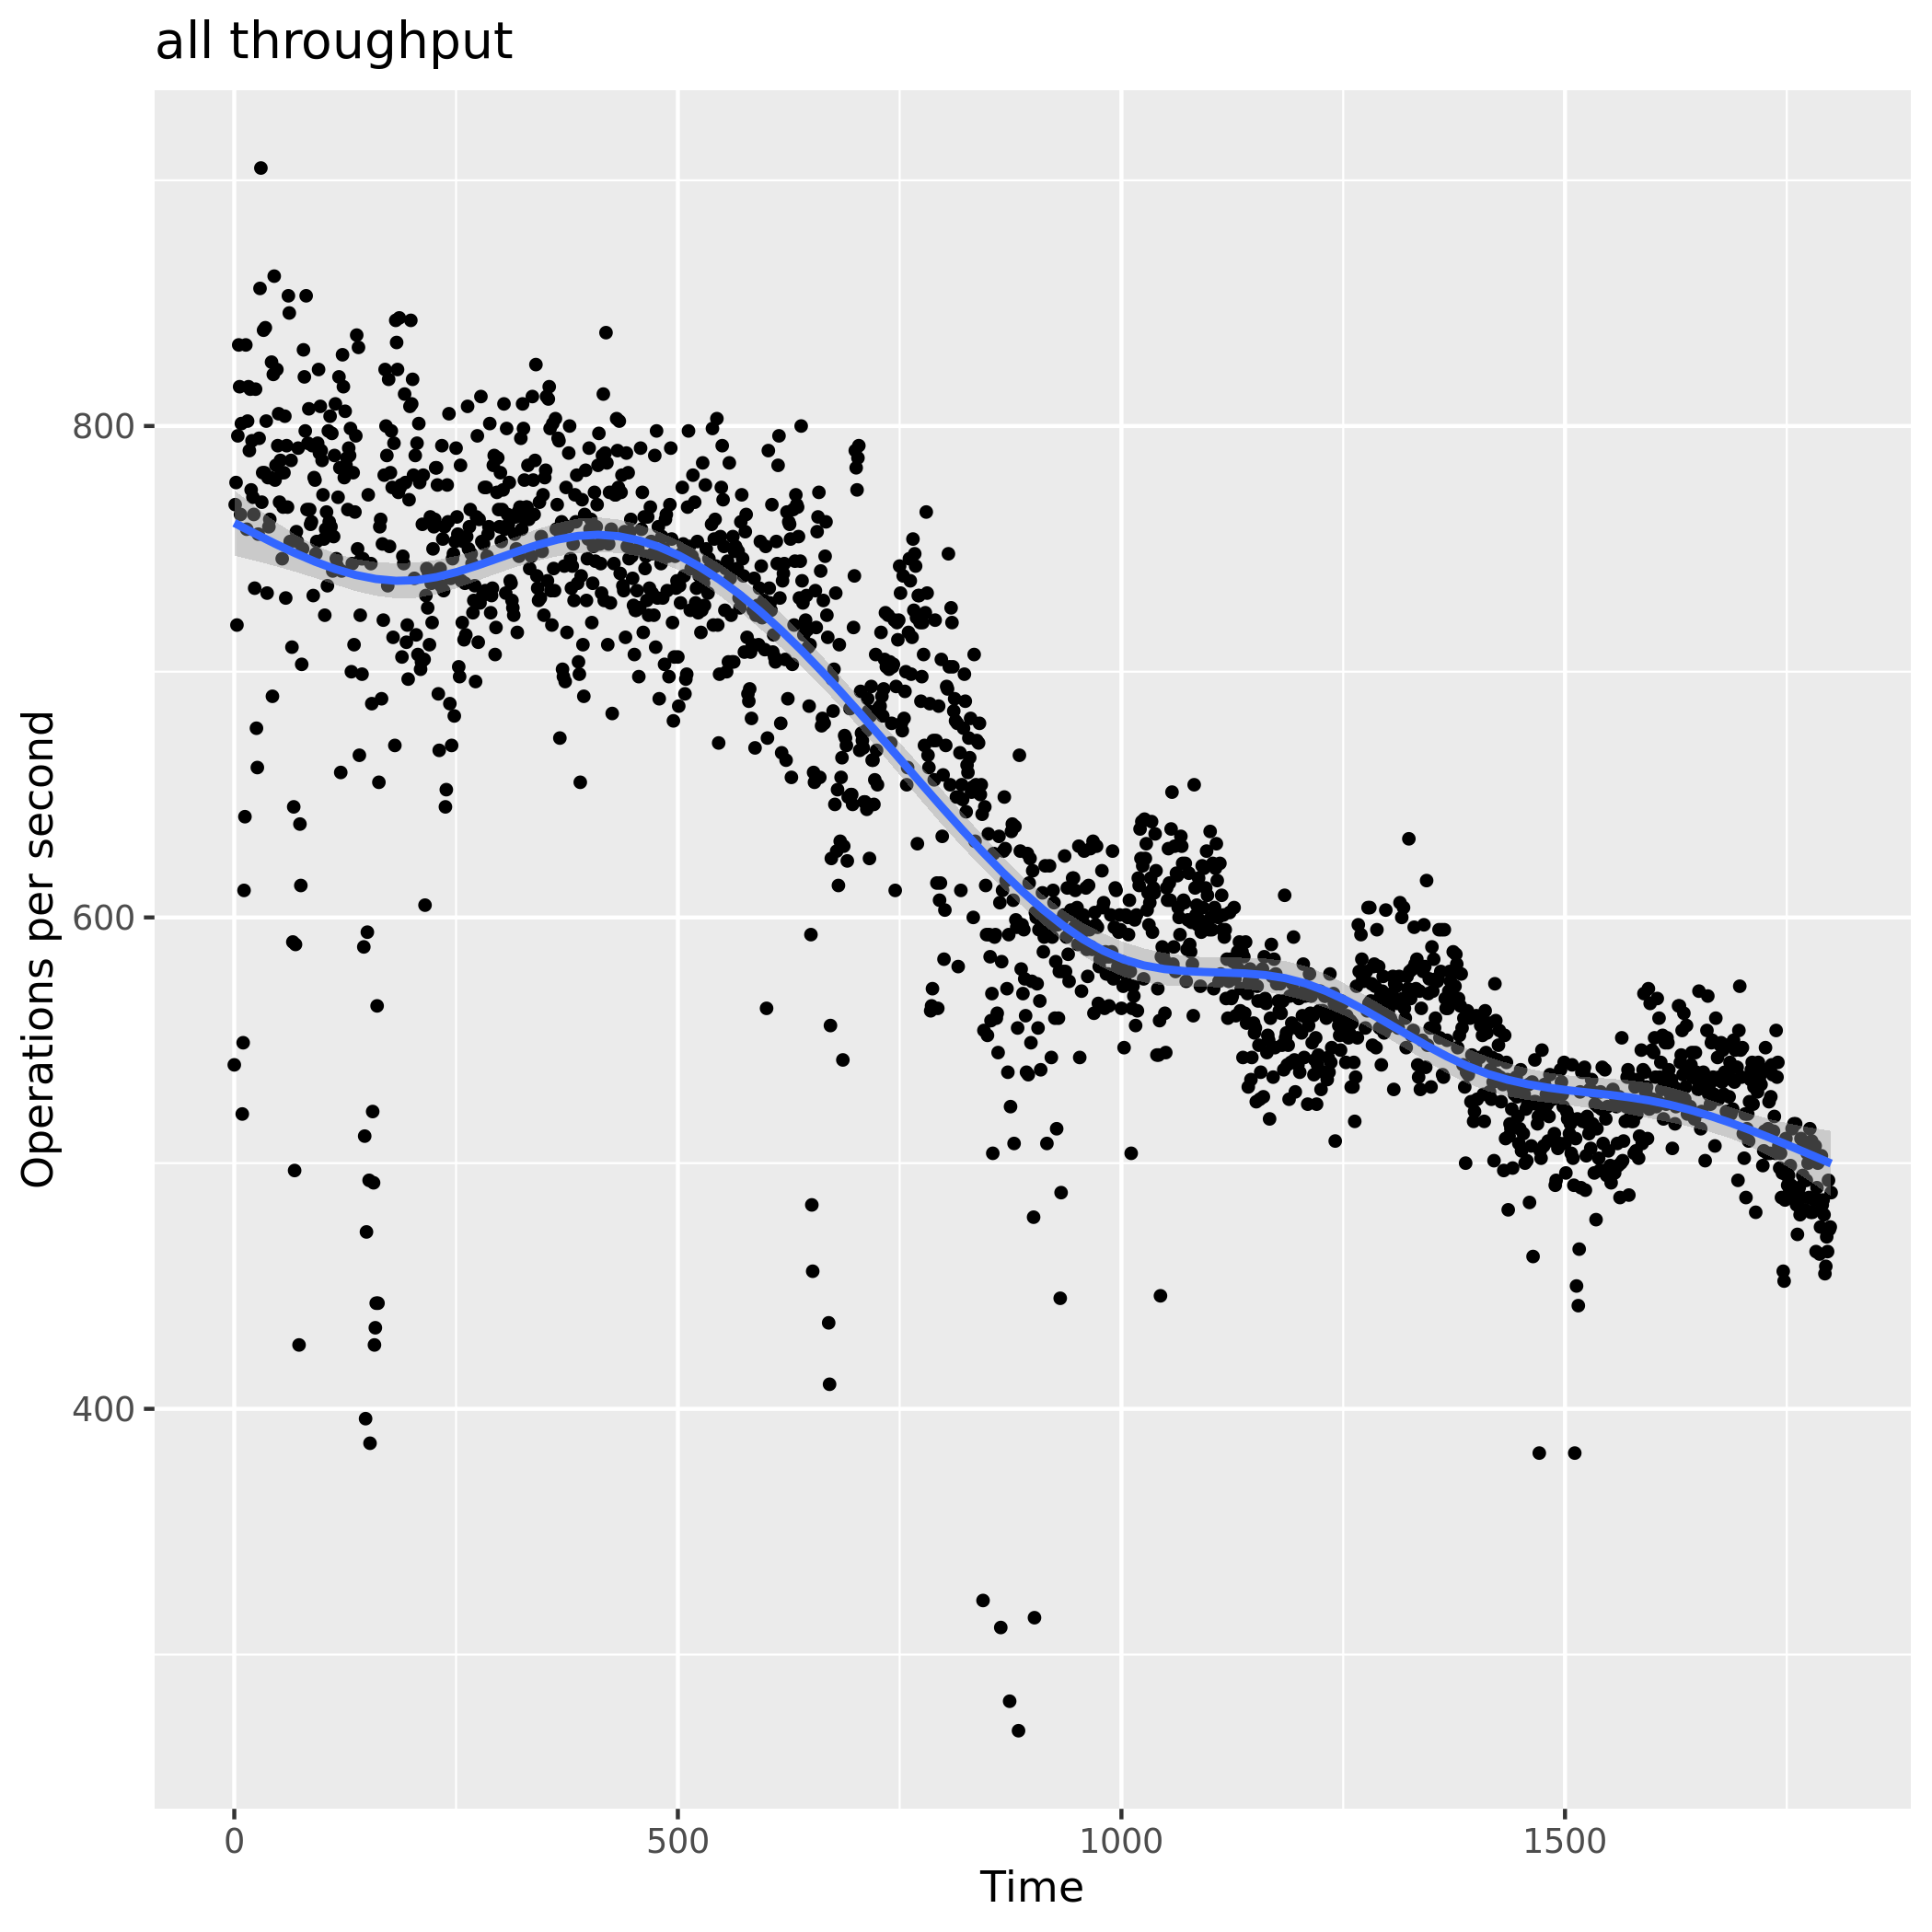
\includegraphics[width=0.8\textwidth]{RandomSlicing_Random_C2_write_heavy_throughput}
	\caption[Throughput for \ac{RS} in C2]{Throughput for \ac{RS} in C2}
\end{subfigure}
\caption[Throughput Comparison]{Throughput Comparison. On the left are the throughput plots of Consistent Hashing, on the right the ones of \ac{RS}.}
\label{fig:throughput_comparison}
\end{figure}
Therefore the hypothesis can be seen as plausible.

\subsubsection{Hypothesis 5}
Hypothesis 5 claims that a system with \ac{RS} will recover faster after a cluster change than with Consistent Hashing.
Again we are using Random Replication as the replication placement strategy to enable a fair comparison.
As the behavior of the throughput during handoff operations is quite unexpected it is hard to tell from its plot when a system has actually recovered.
However, there are clear edges in the latency plots that can be used to approximate the duration of system disruption.
The latency plots of the dynamic runs can be seen in \cref{fig:handoff_comparison}.
\begin{figure}
\begin{subfigure}{0.5\textwidth}
	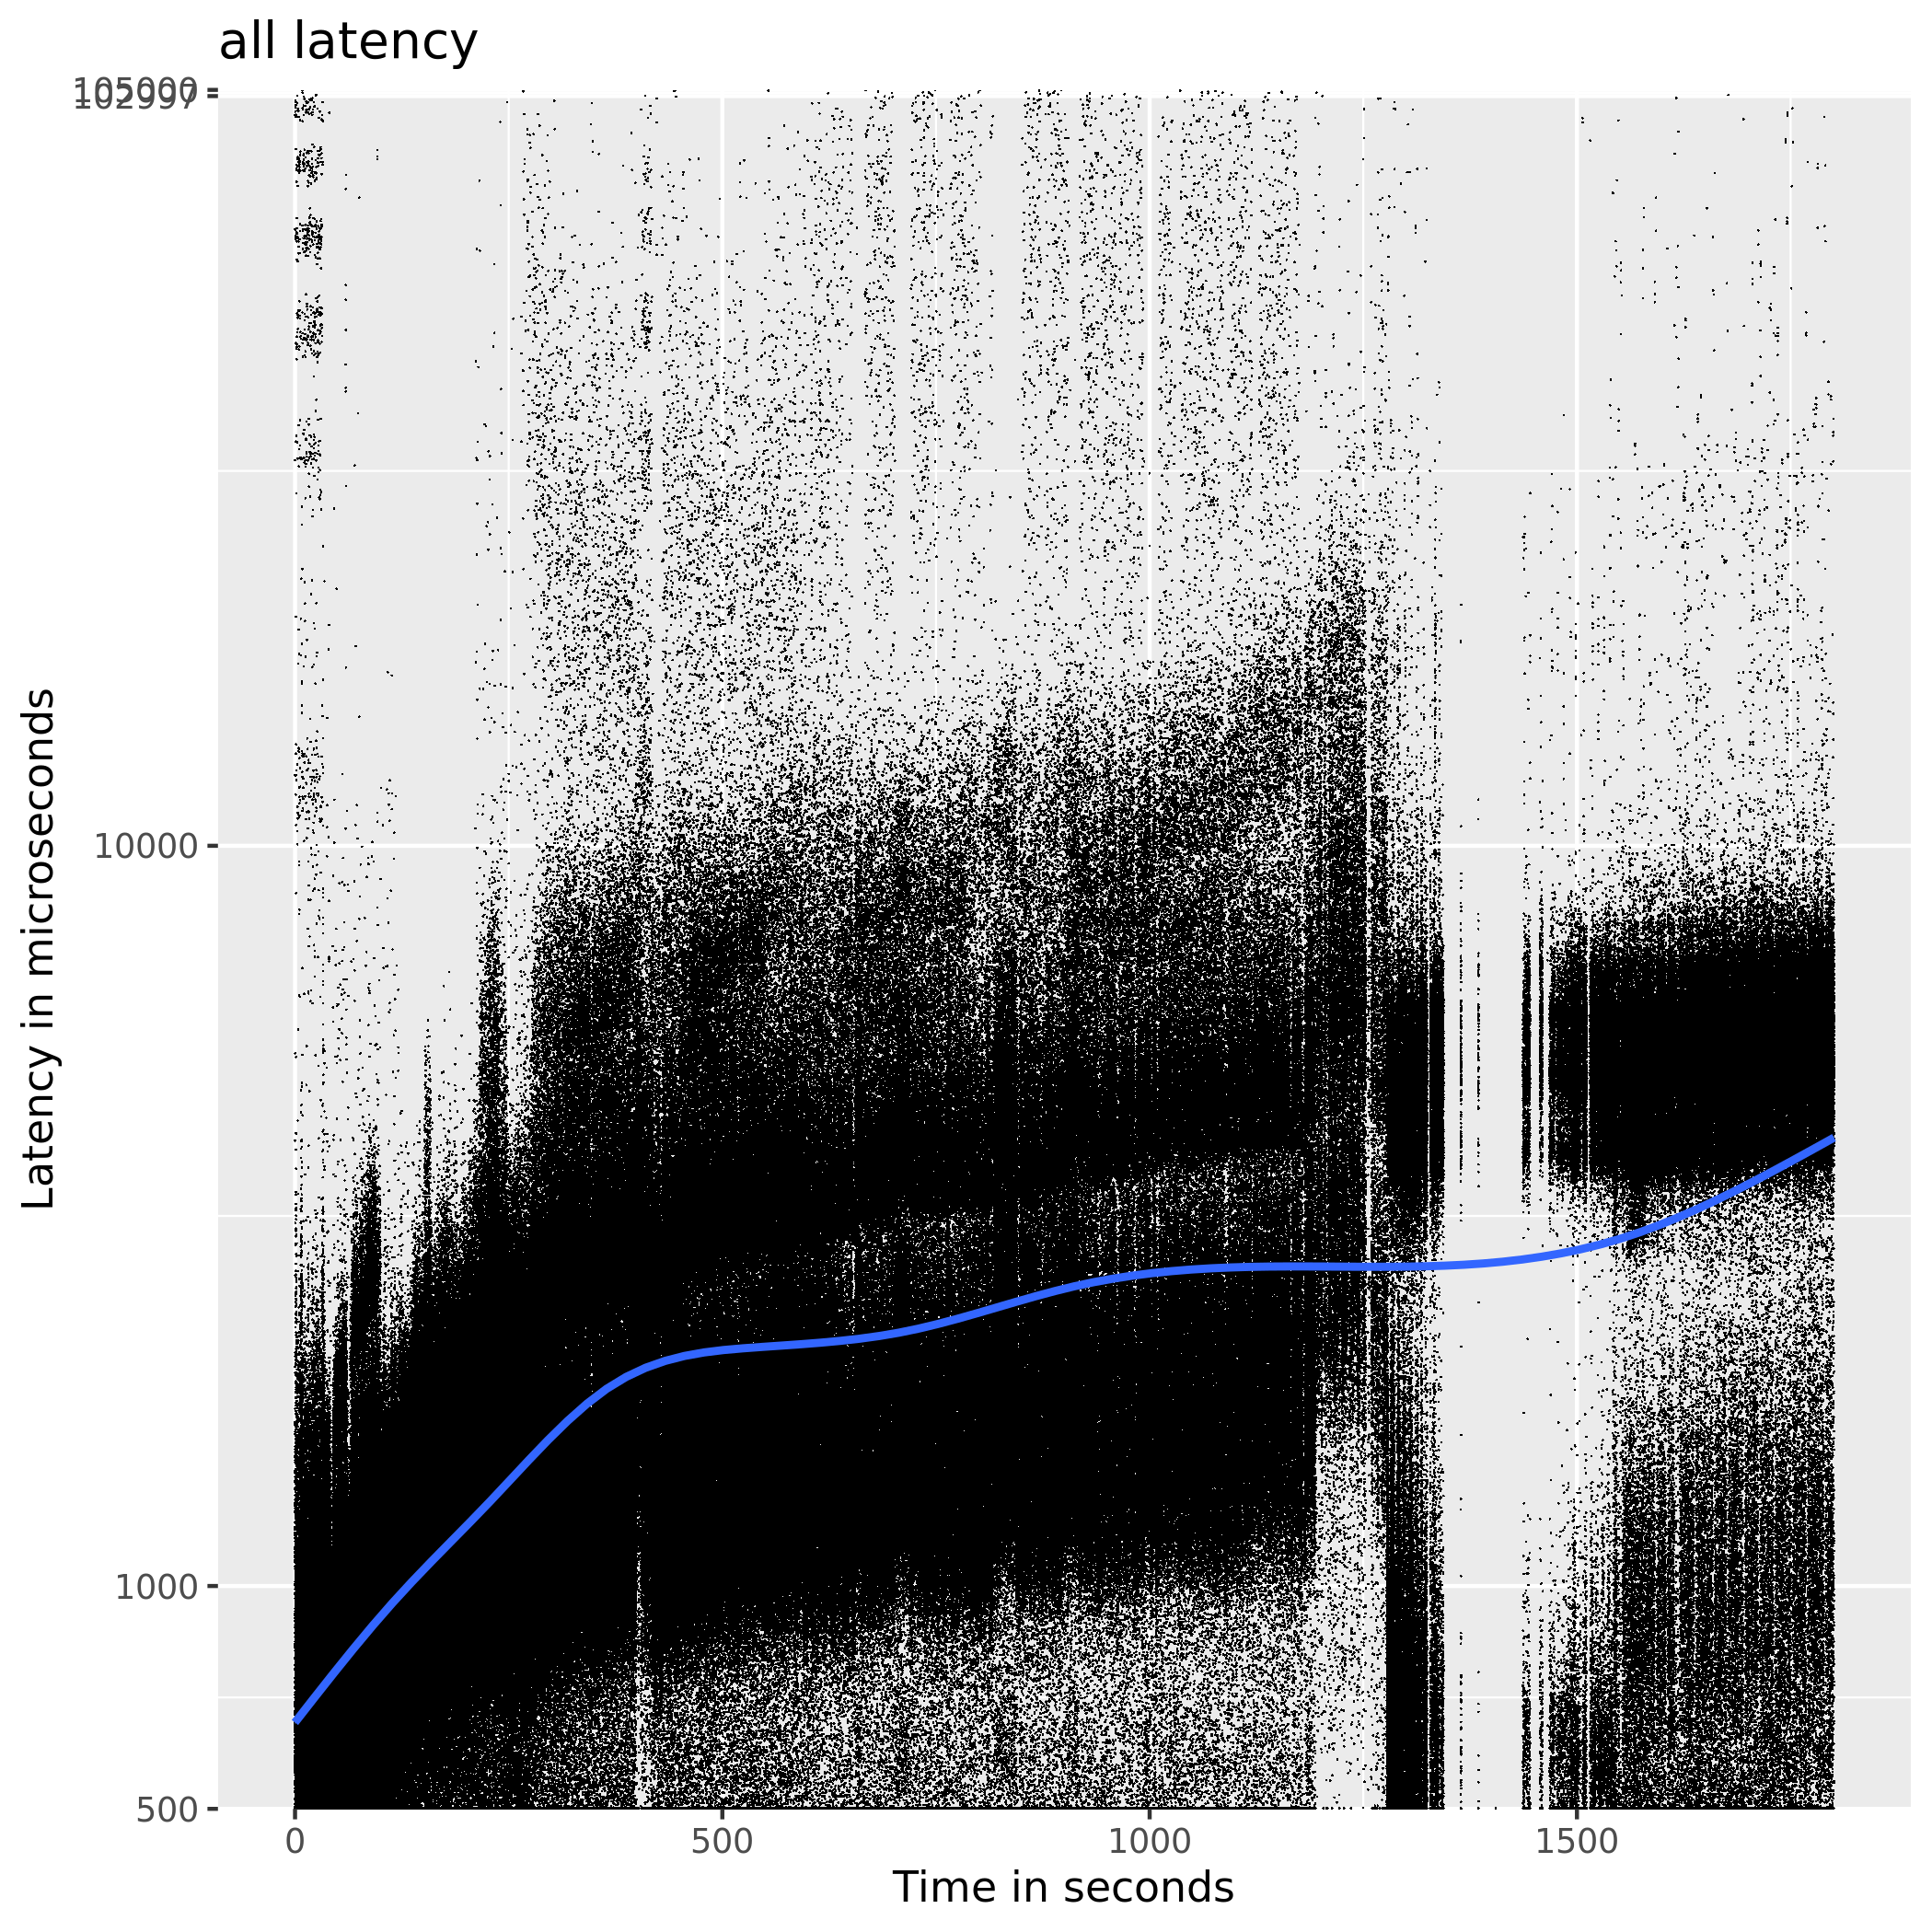
\includegraphics[width=0.8\textwidth]{ConsistentHashing_dynamic_read_heavy_latency}
	\caption[Latency for Consistent Hashing with Read-Heavy Workload]{Latency for Consistent Hashing with Read-Heavy Workload}
\end{subfigure}
\begin{subfigure}{0.5\textwidth}
	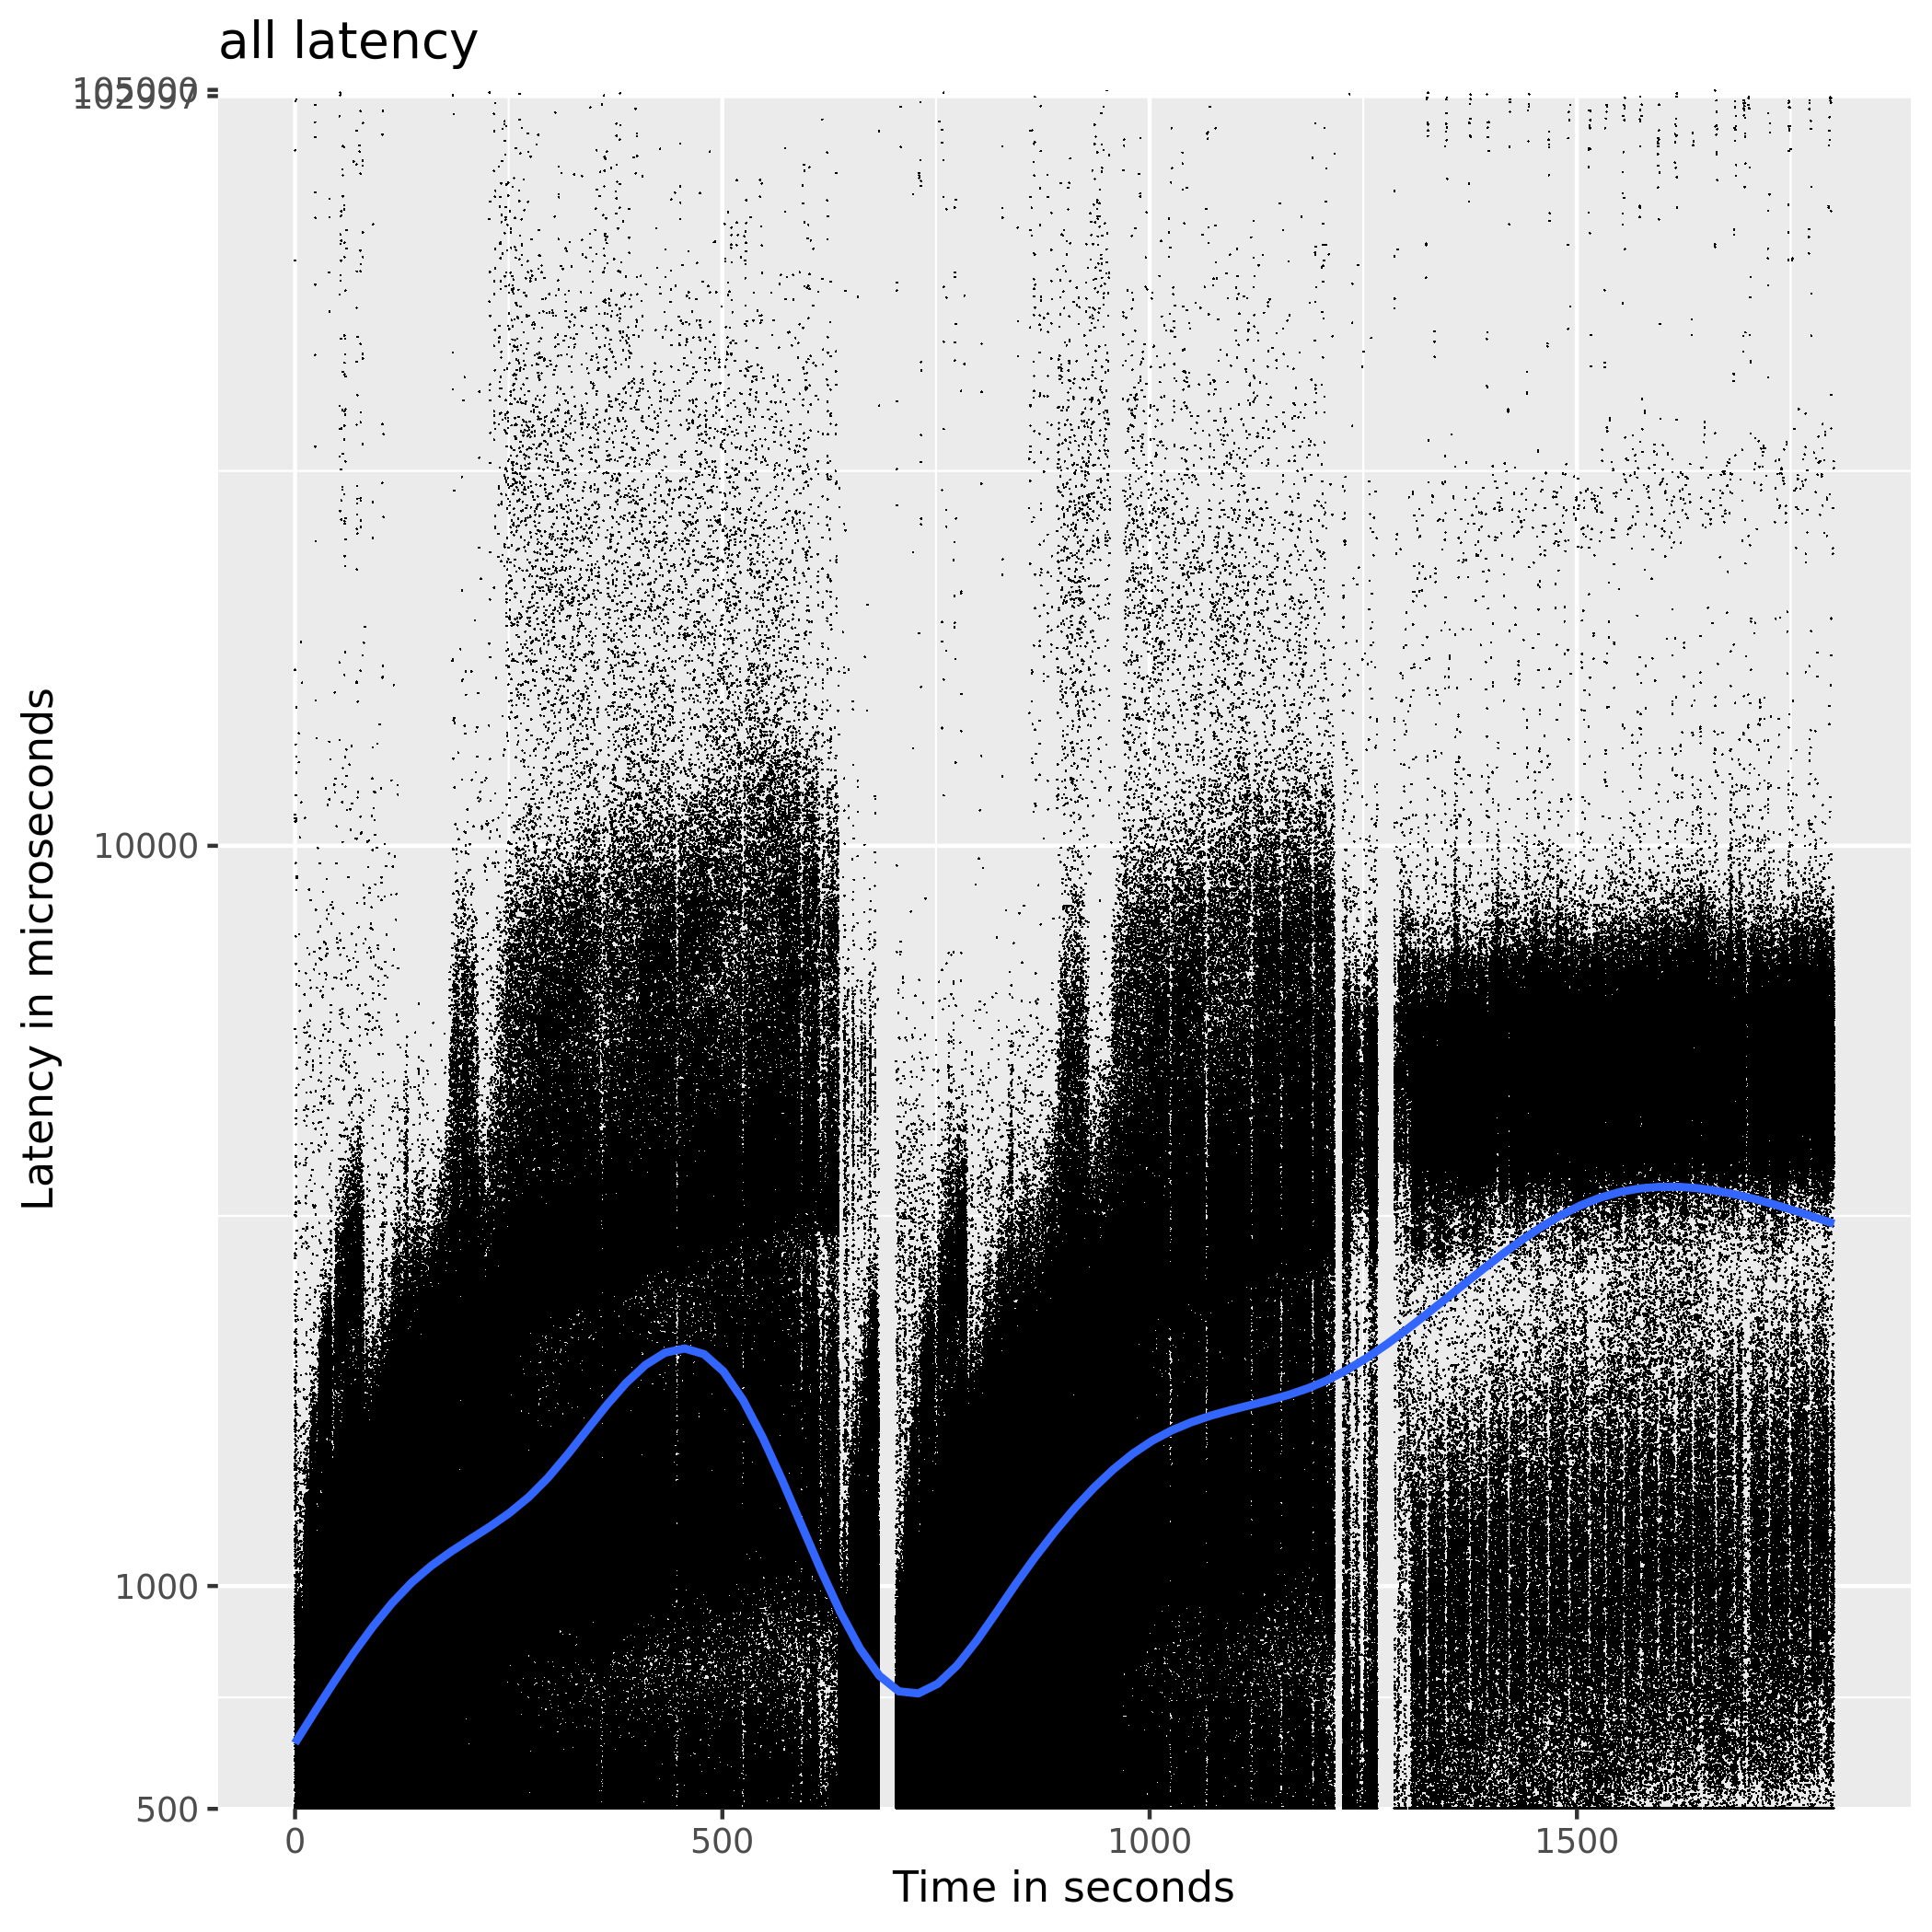
\includegraphics[width=0.8\textwidth]{ConsistentHashing_dynamic_write_heavy_latency}
	\caption[Latency for Consistent Hashing with Write-Heavy Workload]{Latency for Consistent Hashing with Write-Heavy Workload}
\end{subfigure}
\begin{subfigure}{0.5\textwidth}
	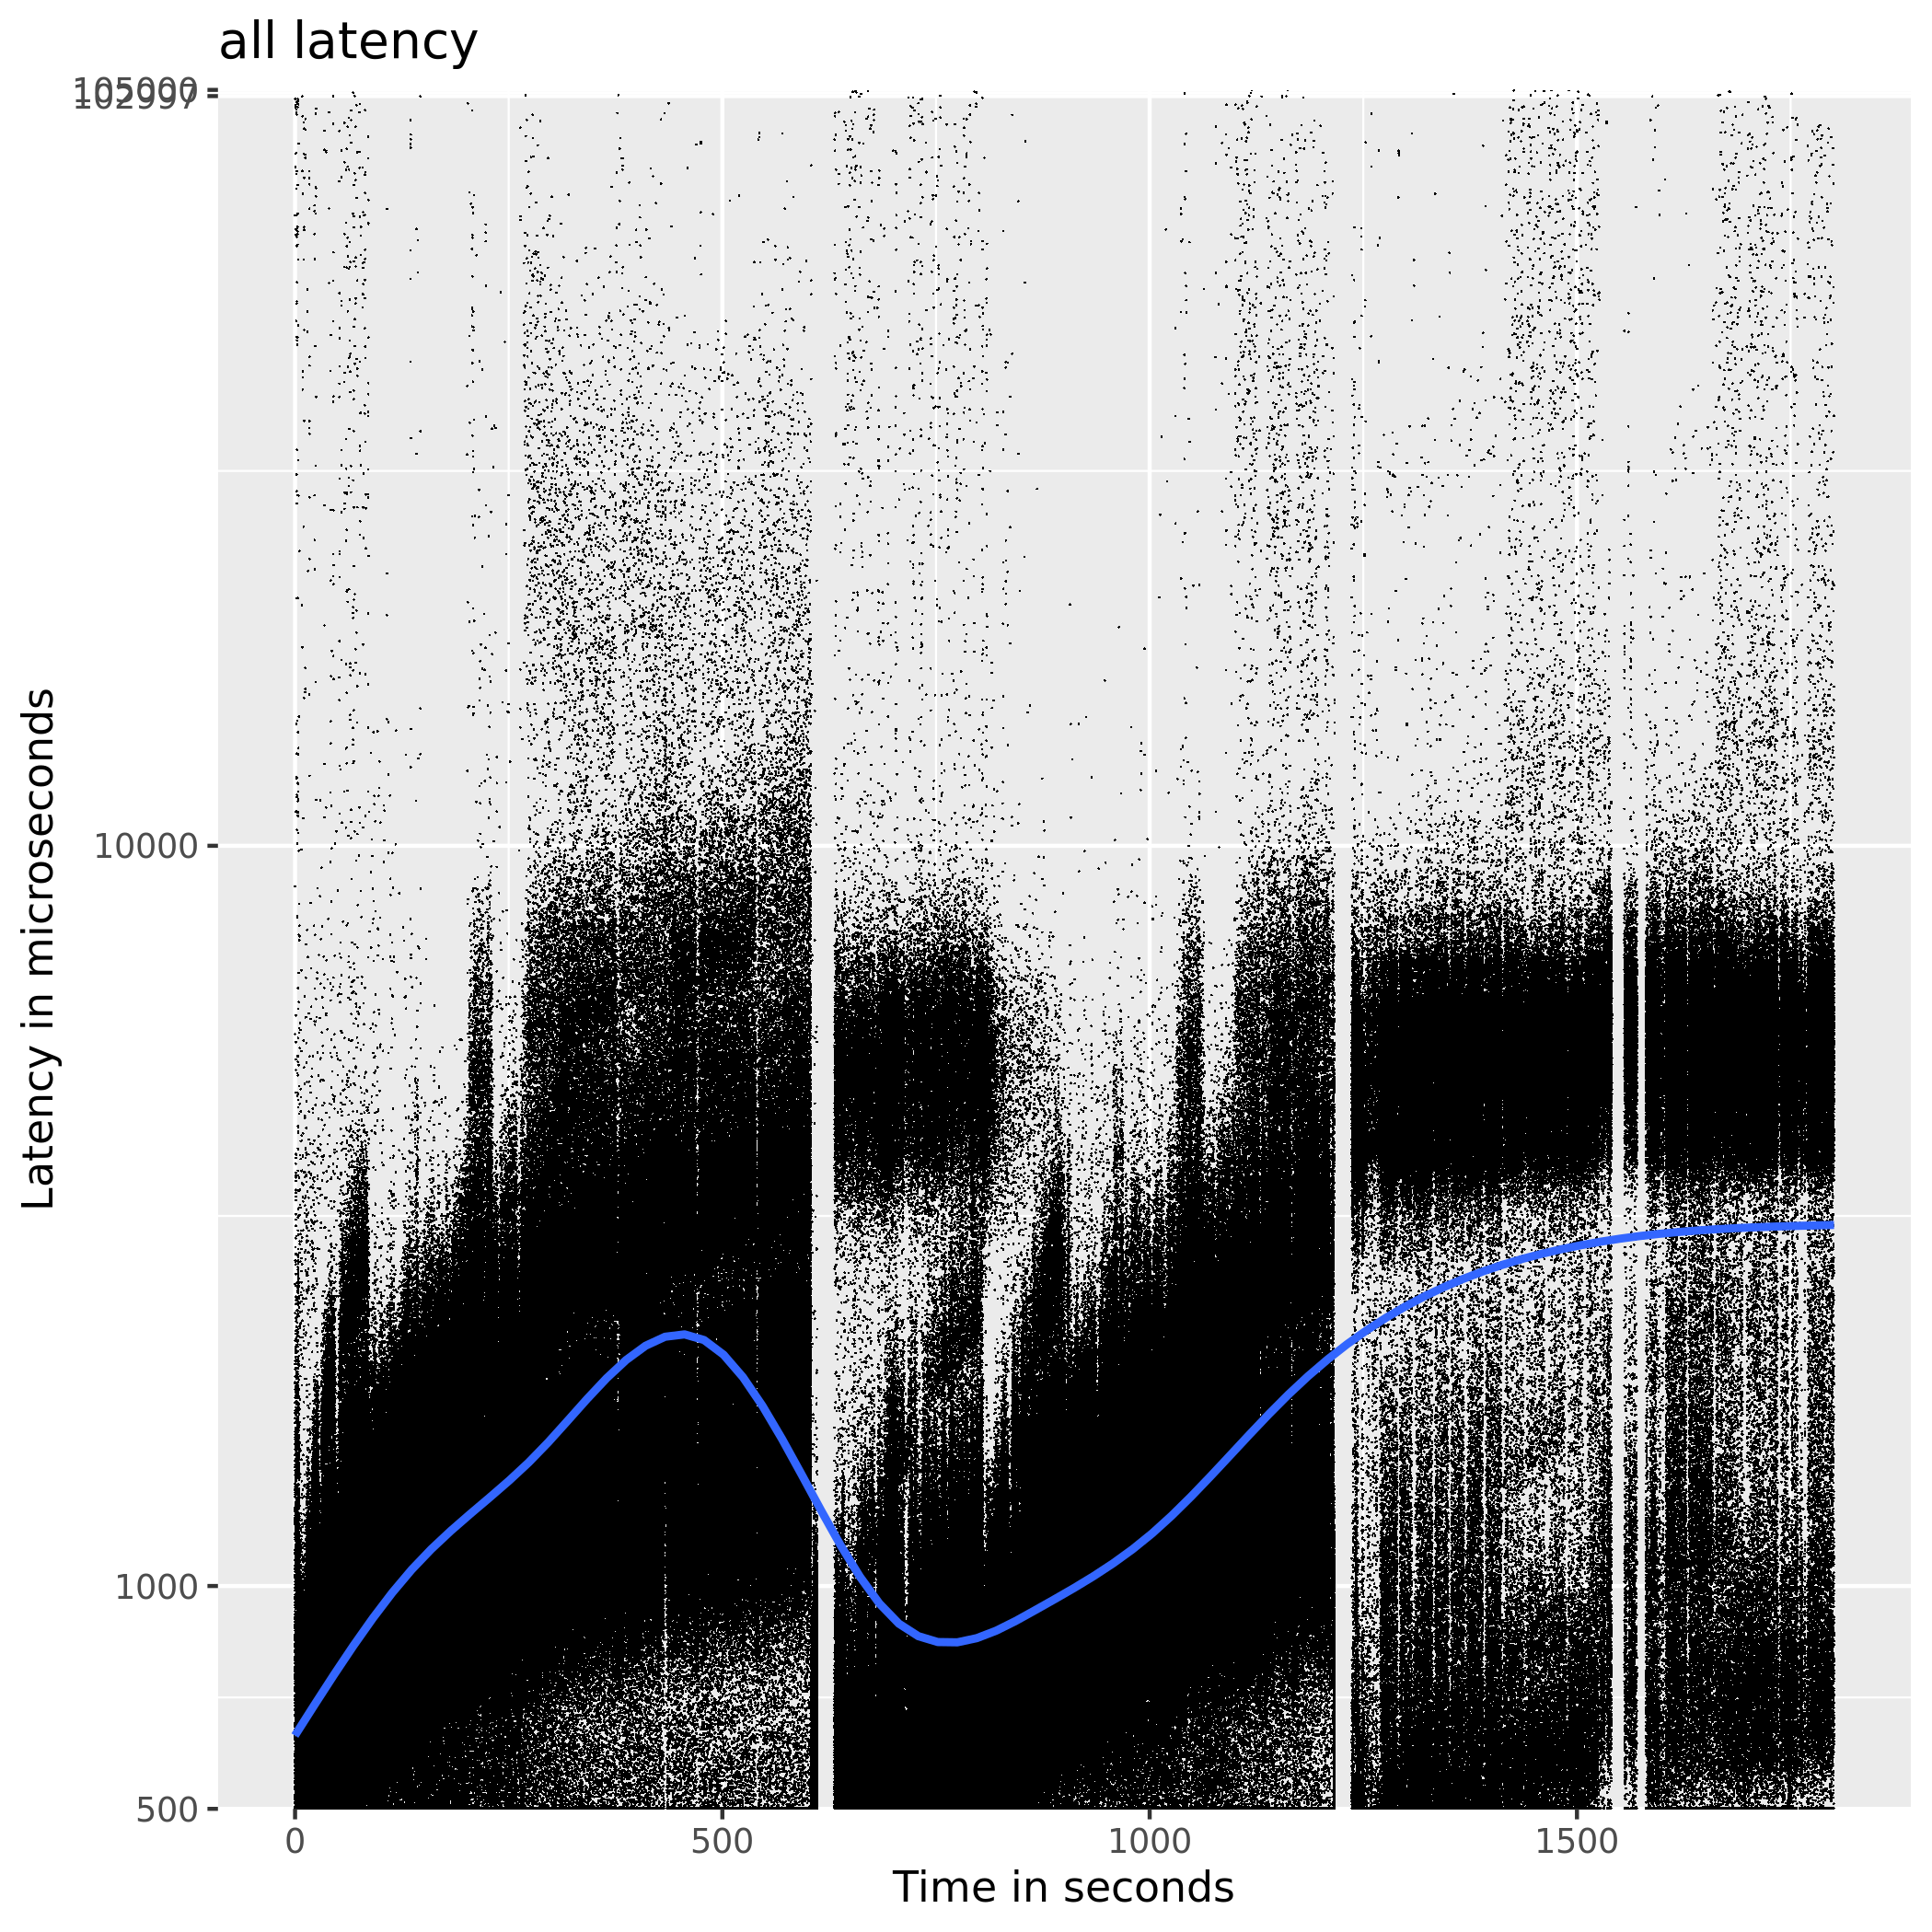
\includegraphics[width=0.8\textwidth]{RandomSlicing_Random_dynamic_read_heavy_latency}
	\caption[Latency for \ac{RS} with Read-Heavy Workload]{Latency for \ac{RS} with Read-Heavy Workload}
\end{subfigure}
\begin{subfigure}{0.5\textwidth}
	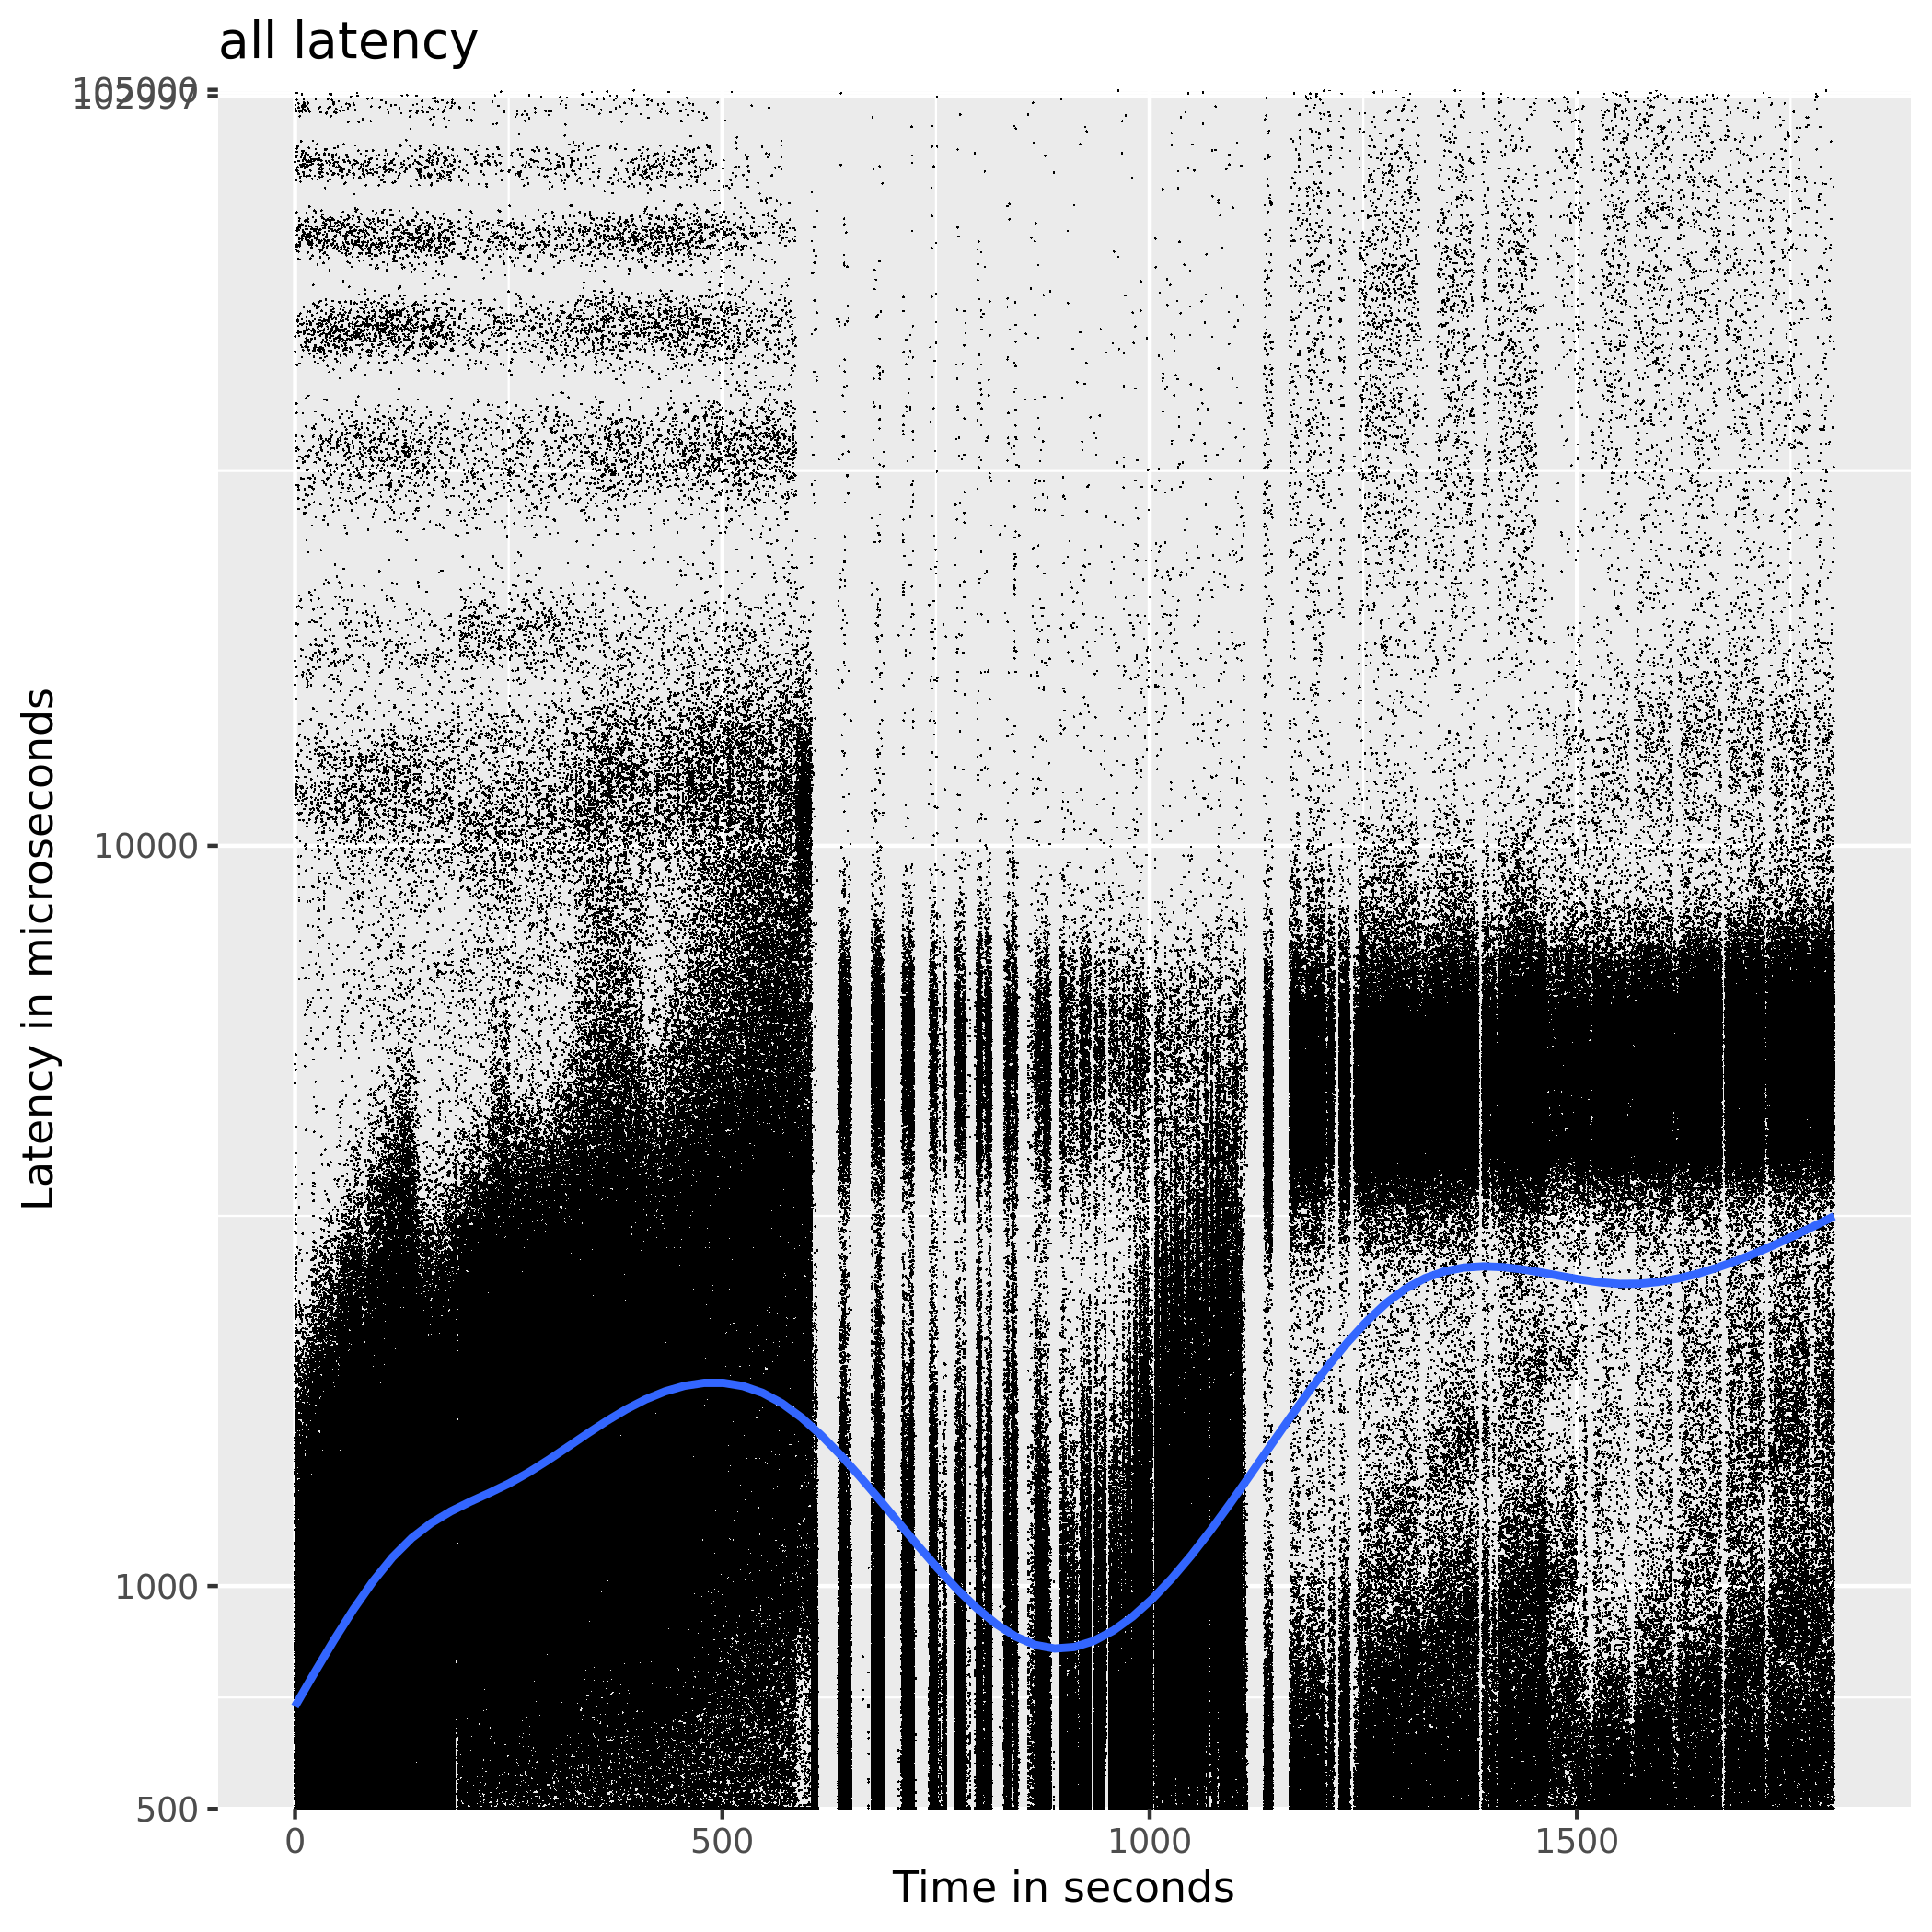
\includegraphics[width=0.8\textwidth]{RandomSlicing_Random_dynamic_write_heavy_latency}
	\caption[Latency for \ac{RS} with Write-Heavy Workload]{Latency for \ac{RS} with Write-Heavy Workload}
\end{subfigure}
\caption[Handoff Comparison]{Handoff Comparison. The hard edges in the latency plot can be used as an index to when the system is disrupted by handoff and repair operations.}
\label{fig:handoff_comparison}
\end{figure}
One can easily see that for the read-heavy workload the disruptions with \ac{RS} are way shorter than with Consistent Hashing.
However, with the write-heavy workload there are multiple small disruptions with \ac{RS} and less and shorter disruptions with Consistent Hashing.
Overall we can make no assertion on the hypothesis with the available data as the results are currently ambiguous and there is a need for more and different kinds of cluster changes to derive a conclusion.

%!TEX root=../master_thesis.tex
\chapter{Future Work}
In this chapter we present future changes to the system that we see as necessary to either improve the system performance or make use of all features of \ac{RS}.
We will list each problem we identify in the current state of the system and then present potential solutions if we already thought of one.

\section{Improve the Gap Collection Algorithm}
The system currently uses a simple greedy gap collection algorithm.
As Miranda et al. show in their evaluation of gap collection algorithms\cite{Miranda2014}, there are alternatives that produce way less gaps without much computation overhead which in turn reduces lookup time.
Especially the large difference for a low number of nodes has a strong impact on systems using Riak Core as they are not expected to scale to a high number of nodes.
Since Riak Core is conceptualized for systems with infrequent cluster changes the lower lookup time will improve the system's throughput.

Another problem we noticed with the gap collection algorithm during the evaluation are some minuscule sections that are results from rounding errors when scaling the weight of the nodes.
As those sections also increase lookup time it is necessary to prevent their creation.
One possible solution is to implement a guard that prevents the creation of sections below a given size which would then also prevent a future feature of creating custom sections for special use cases.
Another solution is to use rational numbers to scale the weights which has a higher memory usage but also higher precision.


\section{Reintegrate Handoff Optimizations}
\ac{RCL} with Consistent Hashing differentiates between different kinds of handoffs to optimize other system procedures and prevent erroneous handoff operations that need to be fixed later.
For example there are different handoff procedures for a simple cluster change and a resize change.
During the proof-of-concept integration of \ac{RS} with \ac{RCL} only a basic handoff workflow was realized.
There are most likely still many corner-cases of cluster changes that could lead to either a failure during handoff or a bad performance during handoff.
As in principle all cluster changes with \ac{RS} lead to a resize handoff the next step is to closely look at how resizing impacts \ac{RCL} with Consistent Hashing and if those corner cases may work with \ac{RS}.
If this is the one can simply adapt the resize handoff for \ac{RS}.
Otherwise the handoff workflow needs to be redesigned completely to handle the new cases brought in by \ac{RS}.


\section{Develop a More Refined \ac{RPS}}
To offer the same functionality with \ac{RS} as with Consistent Hashing, we need to develop a \ac{RPS}.
We presented three simple strategies, Random Replication, Ring Jumping, and Ring Rotation.
The evaluation has shown that none of these is better than replication with Consistent Hashing and show weaknesses when the cluster changes.
Therefore a simple \ac{RPS} may not be feasible with \ac{RS} a more sophisticated approach needs to be developed.
Fritchie\cite{Fritchie2018} proposed to include a level of indirection and map clusters of nodes with a replication strategy to the sections of the ring.
However this then creates the problem of forming these clusters and balancing them, unless we change Riak Core's functionality and leave the replication completely to the implementing system.


\section{Integrate the Replication Placement Strategy with the Preference List Creation}
With Consistent Hashing a complete preference list consisting of all nodes starting at the one owning the key is computed and then split into primary and fallback nodes.
The final preference list is then created by filtering the primary nodes by the ones that are up and inserting fallback nodes when necessary.
The current implementation of the preference list creation with \ac{RS} uses the \ac{RPS} to compute a complete preference list and afterwards filters it in the same way as with Consistent Hashing.
As in most cases not all nodes in the complete preference list are needed calculating the complete preference list creates an overhead.
This overhead is non-existent with consistent hashing as the preference list is simply the underlying data structure of the ring split at the initial node.
With the \acp{RPS} we presented the overhead potentially grows with each additional node that is needed to be appended to the preference list.
Therefore we need to interlace the filtering of the preference list with its computation.
An easy way to achieve this is to change the interface of the replication strategies to offer an iterator-like operation that only computes and returns the next entry of the list.
Instead of filtering the complete preference list we can check the status of each node and poll more nodes if we need to use fallback nodes.


\section{Support Heterogeneous Nodes}
One of the strengths of \ac{RS} over Consistent Hashing is its native support of heterogeneous nodes.
While Amazon's Dynamo implementation\cite{DeCandia2007} offers a support of heterogeneous nodes by assigning each node a different number of sections on the ring this approach can only approximate a balanced distribution of heterogeneous nodes.
With \ac{RS} a more precise balancing of heterogeneous nodes can be achieved.
Currently the support for weights assigned to nodes is implemented in the internal code of the ring component.
However, there is no API to actually specify or change a node's weight.
This seems to be a rather simple change to add a weight parameter to the join operation and implement a new update-weight operation and add it to the stage-plan-commit lifecycle.


\section{Evaluate Higher Scalability}
We only evaluated small cluster sizes with less than ten nodes as is typical for Riak Core applications.
However, Miranda et al. introduce \ac{RS} as a solution for highly scalable replication\cite{Miranda2014}.
Therefore it is interesting to see how in \ac{RCL} Consistent Hashing fares against \ac{RS} when scaling the cluster size to higher values and if it actually enables more use cases as there is no ring size to be set and changed by an admin.

%!TEX root=../master_thesis.tex
\chapter{Conclusion}
In this thesis we gave an overview on the inner workings of \ac{RCL} and its Consistent Hashing implementation.
Inspired by Fritchie's idea to replace the Consistent Hashing algorithm with \ac{RS} we also presented how \ac{RS} works.
Seeing that Consistent Hashing directly allows for a simple and quick \ac{RPS} we also presented a choice of simple \acp{RPS}.
We then implemented a prototype version of \ac{RCL} with \ac{RS} as its data partitioning algorithm and gave an overview of how the structure and some workflows of \ac{RCL} had to be changed.
To compare both versions of \ac{RCL} we designed configurations to illustrate the strengths and weaknesses of both systems.
With those configuration we ran benchmarks to retrieve data.
From that data we created a first impression of how \ac{RS} works with \ac{RCL} and what the big problems are with the current implementation.

This whole process has shown that the choice of the partitioning algorithm in \ac{RCL} is rather an architectural choice than a design one as large parts of the system depend on the inner workings of this algorithm.
In turn, simply replacing the partitioning component and redesigning components directly connected to it is not enough.
One has to rather go back to the architectural phase and reevaluate the design decisions depending on the chosen partitioning algorithm and its requirements, guarantees and other attributes.
Considering \ac{RS} was adopted for \ac{RCL} in a prototype manner without a full-scope design process the evaluation results look promising.
For the tested aspects it produced metrics that were at most slightly worse than \ac{RCL} with Consistent Hashing.
Especially problems during handoff periods and with load balancing can be clearly overcome by a more refined development process in the future.
Overall, we showed that \ac{RS} works as a partitioning algorithm, though it is reliant on its actual gap collection algorithm and replica placement strategy.
We could not show all of the theoretical improvements listed by Fritchie, especially the improvements of the handoff overhead.
However, this was mostly caused by the prototype implementation and missing metrics in the evaluation.
We strongly believe that with a full redesign of affected components and considering our proposed future work \ac{RS} can improve \ac{RCL}'s overall performance and especially its scalability and adaptability in more dynamic clusters.

\printbibliography


\listoffigures

\appendix

%%!TEX root=../master_thesis.tex
\chapter{Components}
\label{chap:components}
In this chapter all modules Riak Core Lite consists of are listed, shortly described, and grouped into logical components.
A visual overview of the components can be found in Figure \ref{fig:components}.
Modules relevant to this thesis 
\begin{figure}
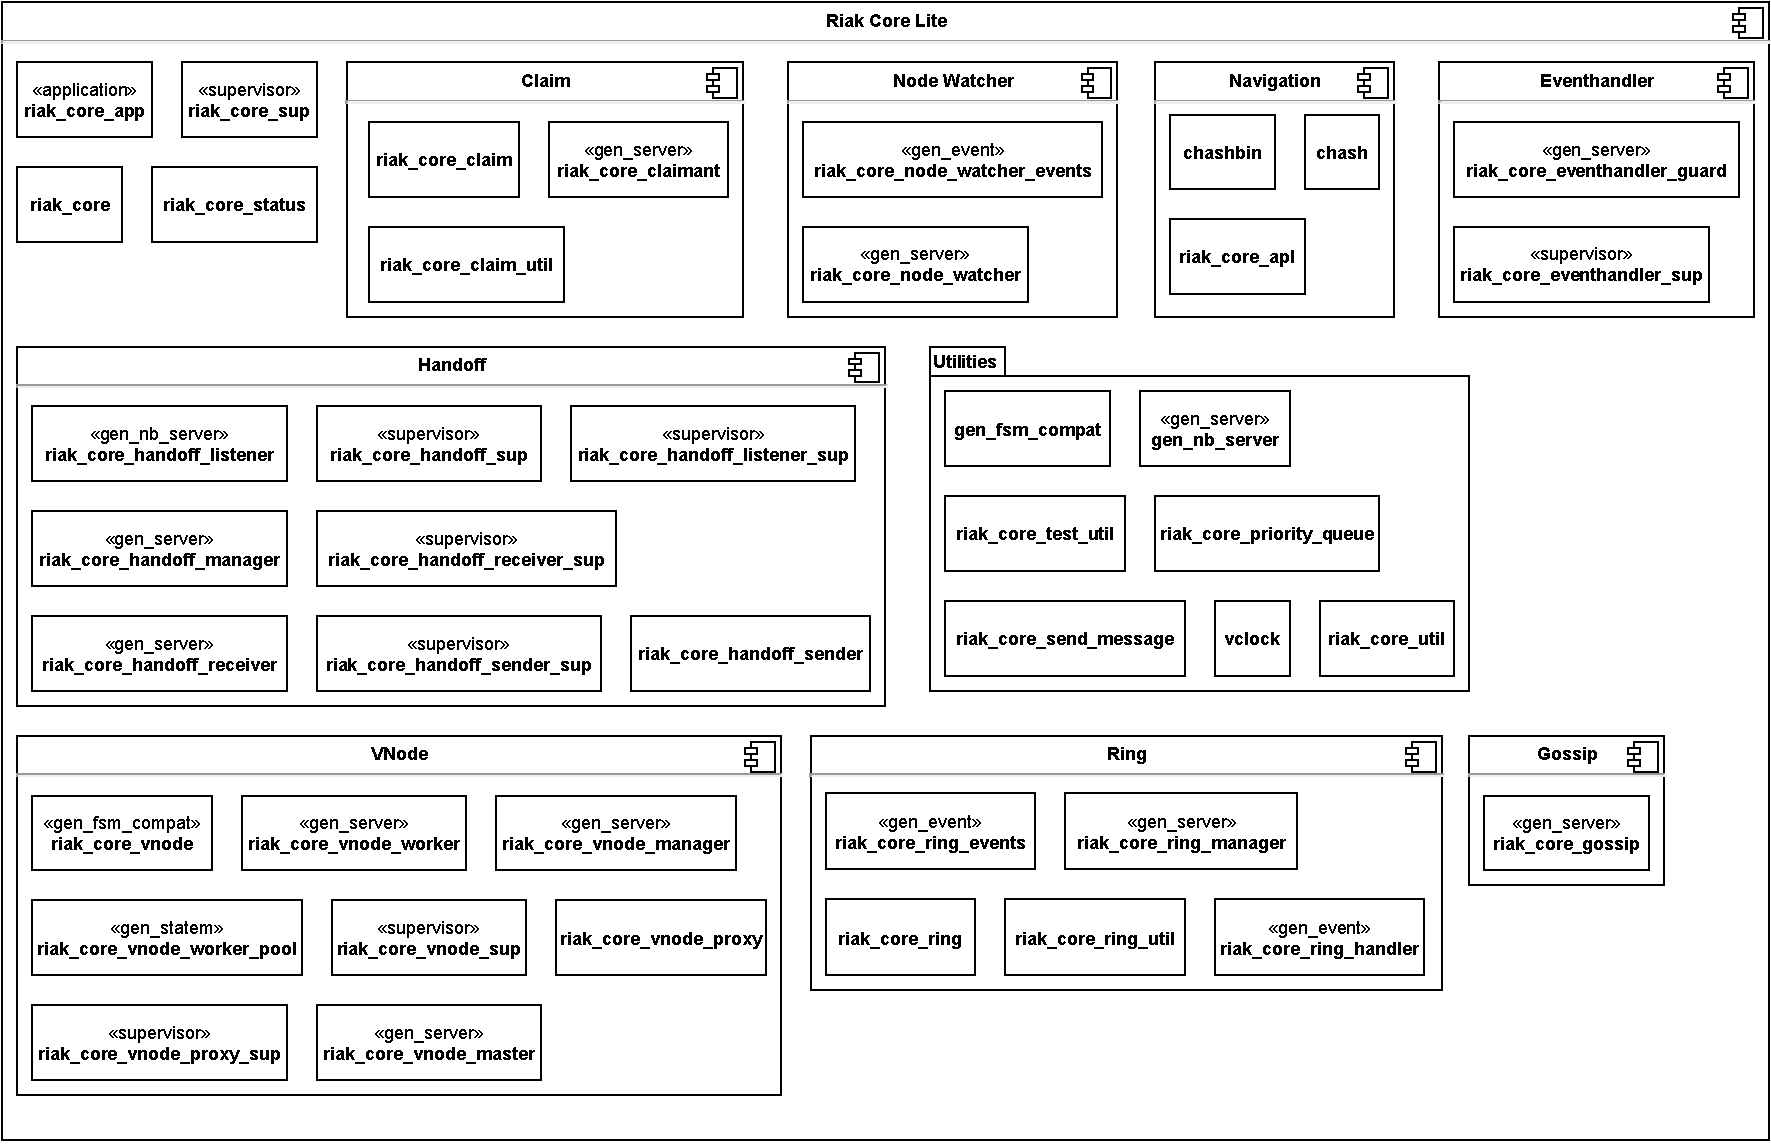
\includegraphics[width=\textwidth]{components}
\caption[System Components]{System Components. Multiple system modules are grouped into logical components to make a superficient description possible.}
\label{fig:components}
\end{figure}

\section{Top Level Modules}
	Top level modules are modules that cannot be assigned to a logical component as their responsibilities lie within a global scope with regard to the system.
	\subsection{riak\_core\_app}
		This module is the entry point to start and stop a system instance.
	
	\subsection{riak\_core\_sup}
		This module is the root Riak Core Lite's supervisor tree and is responsible to keep the system running.
		It exclusively supervises other more specific supervisors.
	
	\subsection{riak\_core}
		The \lstinline!riak_core! module wraps most of the system's core functionality like adding and removing nodes or register applications using the Riak Core instance as a backend.
	
	\subsection{riak\_core\_status}
		This module provides functions to check different information of the system such as the status of the ring or ongoing and scheduled transfers.


\section{Claim}
	In Riak Core Lite the claim system is responsible for managing the ring configuration and updating the ring at appropriate times.
	\subsection{riak\_core\_claim}
		The claim modules implements the claim algorithm.
		This algorithm determines the assignment of sections of the ring to owner nodes such that a sufficiently good load balancing is achieved.
	
	\subsection{riak\_core\_claimant}
		The claimant module is responsible for planning and triggering changes to the cluster and ring.
		There is exactly one claimant service at a time responsible for one ring.
		However, the claimant may change while the system is running.
		The claimant works with a stage-plan-commit model in which first a number of changes like adding nodes or resizing the ring are scheduled for the current claimant.
		Before committing these changes a plan showing the impact of applying those changes.
		When committed, changes are applied to the current ring.
		The claimant is also responsible for deciding when to install the updated ring.
	
	\subsection{riak\_core\_claim\_util}
		This module is a library of utility functions linked to the claim algorithm.

\section{Node Watcher}
	The node watcher component groups components that are responsible for the health of nodes.
	\subsection{riak\_core\_node\_watcher\_events}
		This module allows for event handling implementations for events concerning the health of nodes.
		This can be used to handle a high work load or connectivity issues.
	
	\subsection{riak\_core\_node\_watcher}
		The node watcher provides an interface to retrieve information about the current node health.
	

\section{Navigation}
	The navigation component contains modules concerning the placement of nodes on the ring and replicas on the nodes.
	\subsection{riak\_core\_chashbin}
		This module provides a library to work with a binary encoding of a Consistent Hashing structure that can be used for faster access times.
		The library provides read-only functionality and is mostly used to compute preference lists.
	
	\subsection{riak\_core\_chash}
		A library providing functions to work with a Consistent Hashing structure.
		It can be used to manipulate a structure and access information about the structure.
		The structure stores information of section ownership and is the base for the ring structure.
	
	\subsection{riak\_core\_apl}
		The module \lstinline!riak_core_apl!'s name is short for active preference list.
		It is the entry point to query the system for a preference list containing only nodes that are seen as active by the cluster.
		There are different variants of annotations and filters one can choose to retrieve together with the preference list. 
	

\section{Eventhandler}
	The event handler component contains modules providing utilities for event handlers.
	\subsection{riak\_core\_eventhandler\_guard}
			The event handler guard module can be added to an event handler to guard it from specific events like exit messages that are common to all event handlers.
	
	\subsection{riak\_core\_eventhandler\_sup}
		The event handler supervisor supervises an instance of an event handler guard.
	

\section{Handoff}
	The handoff component component groups the modules responsible for planning, coordinating and executing handoffs.
	Handoffs are data transfers from one node to another happening when a node loses ownership of a section.
	\subsection{riak\_core\_handoff\_listener}
		The handoff listner represents a TCP socket listening to incoming handoffs.
	
	\subsection{riak\_core\_handoff\_sup}
		The handoff supervisor is the root of the supervisor tree concerning the handoffs.
		It supervisors the other supervisor modules.
	
	\subsection{riak\_core\_handoff\_listener\_sup}
		The handoff listener supervisor supervises one handoff listener process.
	
	\subsection{riak\_core\_handoff\_manager}
		The handoff manager is used to manage incoming and outgoing handoffs via handoff senders and receivers, and monitors ongoing handoffs.
		It limits the concurrently active handoffs and is also able to abort  handoffs.
	
	\subsection{riak\_core\_handoff\_receiver\_sup}
		The handoff receiver supervisor supervises one handoff receiver.
	
	\subsection{riak\_core\_handoff\_receiver}
		The handoff receiver handles incoming handoff messages.
		Depending on the message it triggers a handoff on the node or only updates the state.
	
	\subsection{riak\_core\_handoff\_sender\_sup}
		The handoff sender supervisor supervises one handoff sender worker.
		The child has to be started via this supervisor and initializes the sender process.
	
	\subsection{riak\_core\_handoff\_sender}
		The handoff sender is responsible for transferring the data currently owned by the node to the new owner.
		The sending process is a folding operation over the affected data.
	

\section{VNode}
	The vnode component groups all modules concerning the representation and handling of a node and the organization of the cluster.
	\subsection{riak\_core\_vnode}
		The vnode module is a behavior module representing a node in the cluster.
		This is the main entry point of defining the application specific behavior of the system as the callbacks allow to react to different events in the system, like different milestones in the handoff life-cycle.
	
	\subsection{riak\_core\_vnode\_worker}
		The vnode worker module allows for process to be created to handle a task of a node.
	
	\subsection{riak\_core\_vnode\_manager}
		The vnode manager is the entry point to manage the view of the cluster via vnodes.
		It handles the registering and unregistering of nodes as well as the initialization and balancing of handoff transfers.
	
	\subsection{riak\_core\_vnode\_worker\_pool}
		The worker pool manages the schedule work tasks and assigns worker processes to tasks.
	
	\subsection{riak\_core\_vnode\_sup}
		The vnode supervisor supervises one vnode and also handles a controlled shutdown to enable shutting down the worker pool properly.
	
	\subsection{riak\_core\_vnode\_proxy}
		The vnode proxy receives messages and handles an inbox and an overflow of messages.
	
	\subsection{riak\_core\_vnode\_proxy\_sup}
		The vnode proxy supervisor supervises the vnode proxies.
		Additional proxies need to be started via the supervisor.
	
	\subsection{riak\_core\_vnode\_master}
		The vnode master allows to dispatch requests and tasks to nodes.
		It sends those requests to the proxy belonging to the intended node.
	

\section{Ring}
	The ring component groups modules responsible for representing, manipulating, maintaining, and querying the ring.
	\subsection{riak\_core\_ring\_events}
		The ring events module is the implementation of an event handler concerning ring events such as a ring update.
	
	\subsection{riak\_core\_ring\_manager}
		The ring manager gives access to the single installed ring of the system.
		The install ring is the version of the ring seen as the currently correct version.
		It can be changed via the ring manager.
		The ring is stored both in memory as well as in a persistent ring file.
		One can also retrieve alternative representations of the ring like the chashbin structure.
	
	\subsection{riak\_core\_ring}
		This module represents the core library to handle the ring.
		It allows to modify the cluster by adding and removing members as well as their meta data.
		The state of the ring consists of the ring owner, current vector clock, chash structure, ring meta, a list of pending changes, cluster members and their meta data, the name of the current claimant, a list of seen updates per node, and the current ring version.
		The module provides a library to access most of this information in raw or processed form.
	
	\subsection{riak\_core\_ring\_util}
		The ring util module provides a library consisting of function useful to the ring modules but not necessarily bound to the ring like hashing a partition id.
	
	\subsection{riak\_core\_ring\_handler}
		The ring handler is an event handler responding to a ring update and reconfiguring the vnode proxies.
	

\section{Gossip}
	The gossip component groups all components responsible for implementing the gossip protocol which leads to an eventually consistent state.
	\subsection{riak\_core\_gossip}
		The sole module responsible for implementing the gossip protocol provides different functions to communicate the ring state between nodes.
		The random gossip protocol is one variant, alternatively the ring can also be sent to a targeted node.
		When a node is removed from the cluster the gossip module is responsible of informing it and other members.
	

\section{Utilities}
	As one can see utilities are not grouped in a component but rather in a package as the member modules do not necessarily have any cohesion between each other.
	Utilities rather group modules implementing common concepts.
	\subsection{riak\_core\_util}
		Riak Core utilities form a library handling a multitude of tasks such as  RPC, starting application dependencies, or creating a handoff fold request from handoff data.
	
	\subsection{riak\_core\_send\_message}
		Send message is the implementation of a message sending system that does not block the sender based on modified OTP concepts.
	
	\subsection{riak\_core\_priority\_queue}
		The priority queue module implements a priority queue based on the necessary functions offered by erlang's queue module.
	
	\subsection{riak\_core\_test\_util}
		THe test utilities include functions to set up test cases like creating a mock ring or stopping processes.
	
	\subsection{gen\_fsm\_compat}
		THis module implements a modified state machine behavior.
	
	\subsection{vclock}
		This module implements a standard vector clock.
	
	\subsection{gen\_nb\_server}
		This module is a minimal implementation of erlang's \lstinline!gen_server! behavior module.

%!TEX root=../master_thesis.tex
\chapter{Actions}

\section{General Actions}
\begin{actionbox}{Send Ring}{send_ring}
	\begin{action}
		\call{riak_core_gossip:send_ring/2} If the sending node owns gossip tokens it sends its ring to another node where both rings are reconciled.
		\begin{action}
			\call{riak_core_ring_manager:get_raw_ring/0} Retrieve the raw ring that is to be sent out.
			\call[\actiontag{action}]{Check Tainted} See Action \ref{action:check_tainted}.
			\call[\actiontag{rpc}]{riak_core_gossip:reconcile_ring/1} Reconcile the received ring with the local ring.
			\begin{action}
				\call[\actiontag{action}]{Transform Ring, alt=reconciled_ring} Apply the reconcile callback to the local ring. See Action \ref{action:transform_ring}.
				\begin{action}
					\call[\actiontag{callback}\actiontag{action}]{Reconcile} See Action \ref{action:reconcile}.
				\end{action}
			\end{action}
		\end{action}
	\end{action}
\end{actionbox}

\begin{actionbox}{Transform Ring (alt = new\_ring | reconciled\_ring | ignore)}{transform_ring}
	\begin{action}
		\call{riak_core_ring_manager:ring_trans/2} Transforms the current ring with the given callback.
		Depending on the callback the new state is gossiped randomly or deterministic or only set locally.
		\begin{action}
			\call[\actiontag{callback}]{Callback} The transformation callback that is applied to the ring. The result tuple contains the alt-value.
			\call[\actiontag{action}]{Check Tainted} See Action \ref{action:check_tainted}.
			\call[\actiontag{action}]{Set Ring} Sets the new ring in the ETS table.
			See Action \ref{action:set_ring}.
			\call{riak_core_ring:update_meta/3} Updates the meta entry and its timestamp if the value differs.
			\call[\actioninfo{ignored for alt=set\_only}]{riak_core_ring_events:ring_update/1} Applies the update callback to the current ring.
			\call[\actioninfo{alt=new\_ring $\to$ random; alt=set\_only $\to$ ignore; alt=reconciled\_ring $\to$ not random}]{riak_core_gossip:\{random_\}recursive_gossip/2} Gossips the state to the children of a given node.
			 For random recursive gossip the gossiping node is chosen at random.
			\begin{action}
				\call{riak_core_ring:active_members/1} Retrieves all members whose status is joining, valid, leaving, or exiting.
				\call[\actioninfo{for each active member}\actiontag{action}]{Send Ring} See Action \ref{action:send_ring}.
			\end{action}
		\end{action}
	\end{action}
\end{actionbox}

\begin{actionbox}{Check Tainted}{check_tainted}
	\begin{action}
		\call{riak_core_ring:check_tainted/2} Checks if the tainted-flag is set in the meta data.
		Either stops the application with a given error message or just logs the error message when the ring is tainted.
		\begin{action}
			\call[\actioninfo{If ring is tainted}]{riak_core:stop/1} Stops the application and logs the given reason.
		\end{action}
	\end{action}
\end{actionbox}

\begin{actionbox}{Ring Changed}{ring_changed}
	\small
	\begin{action}
		\call{riak_core_claimant:ring_changed/2} Applies changes to the ring and informs other nodes.
		\begin{action}
			\call{riak_core_ring:members/2} Check for joining members.
			\call{riak_core_ring:members/2} Check for valid and leaving members.
			\call{riak_core_ring:claimant/1} Retrieve claimant to check if it is a valid member.
			\call{riak_core_ring:set_claimant/2} If the claimant is missing set the next claimant.
			\call{riak_core_ring:increment_ring_version/2} Update the ring version if the claimant was changed.
			\call{riak_core_ring:members/2} Find joining members.
			\call{riak_core_ring:get_member_meta/3} Retrieve meta to filter for auto joining nodes.
			\call{riak_core_ring:claimant/1} Retrieve current claimant.
			\call{riak_core_ring:set_member/5} Set all joining nodes as valid members.
			\call{riak_core:cluster_name/1} Retrieve current cluster name.
			\call{riak_core_ring:members/2} Retrieve exiting members.
			\call{riak_core_ring:members/2} Retrieve invalid members.
			\call[\actiontag{action}]{Refresh Ring} Inform each exiting node and refresh their ring to a fresh ring only containing themselves.
			See Action \ref{action:refresh_ring}
			\call{riak_core_ring:claimant/1} Retrieve current claimant to check if the local node is the claimant.
			\call{riak_core_ring:pending_changes/1} Retrieve pending changes from old state.
			\call{riak_core_ring:pending_changes/1} Retrieve pending changes from changed state.
			\call{riak_core_ring:cluster_name/1} Find out if the cluster name is set.
			\call[\actiontag{rpc}]{riak_core_ring_manager:set_cluster_name/1} If the cluster name is not set, set the cluster name for every member.
		\end{action}
	\end{action}
\end{actionbox}

\begin{actionbox}{Refresh Ring}{refresh_ring}
	\begin{action}
		\call{riak_core_ring_manager:refresh_ring/2} Refreshes the ring on the given node to a ring containing only that node and puts the result into the ETS table and ring file.
		\begin{action}
			\call{riak_core_ring:fresh/0} Create a new ring state.
			\begin{action}
				\call{chash:fresh/2} Create a new chash structure with the given node as the owner.
			\end{action}
			\call[\actiontag{action}]{Set Ring} Sets the ring in the ETS table.
		\end{action}
	\end{action}
\end{actionbox}

\begin{actionbox}{Reconcile}{reconcile}
	\begin{action}
		\call{riak_core_gossip:reconcile/2} Reconciles two diverged rings into one.
		\begin{action}
			\call{riak_core_ring:reconcile_names/2} If one name is undefined the result is undefined, else a term consisting of both names is returned.
			\call{riak_core_ring:owner_node/1} Retrieve the owner of the other ring.
			\call{riak_core_ring:reconcile_members/2} Reconciles members and their status of both rings using vector clocks.
			\call{riak_core_ring:cluster_name/1} Get first ring's name for comparison.
			\call{riak_core_ring:cluster_name/1} Get other ring's name for comparison.
			\call{riak_core_ring:member_status/2} Get status of other ring's owner before reconciliation.
			\call{riak_core_ring:reconcile/2} Merges all ring attributes.
			\begin{action}
				\call[\actiontag{action}]{Check Tainted} Check other ring tainted.
				See Action \ref{action:check_tainted}.
				\call[\actiontag{action}]{Check Tainted} Check my ring tainted.
				See Action \ref{action:check_tainted}.
			\end{action}
			\call{riak_core_ring:member_status/2} Get status of other ring's owner in reconciled ring.
			\call{riak_core_ring:ring_changed/2} Apply changes to the ring.
			\begin{action}
				\call[\actiontag{action}]{Check Tainted} See Action \ref{action:check_tainted}.
				\call[\actiontag{action}]{Ring Changed} Apply changes to the ring.
				See Action \ref{action:ring_changed}.
			\end{action}
			\end{action}
	\end{action}
\end{actionbox}

\begin{actionbox}{Set Ring}{set_ring}
	\begin{action}
		\call{riak_core_ring_manager:set_ring/2} Set the ring in the ETS table.
		\begin{action}
			\call{riak_core_ring:set_tainted/1} Set the ring as tainted to check for leaks over gossip.
		 	\call{riak_core_ring:chash/1} Get the chash from the ring.
		 	\call{chashbin:create/1} Compute the chashbin from the ring.
		\end{action}
	\end{action}
\end{actionbox}


\begin{actionbox}{Do Claimant}{do_claimant}
	\begin{action}
		\call{riak_core_claimant:do_claimant/5} Handle joining nodes and add them to the ring.
		If there are no joining nodes apply transfers to the ring.
		Finally handle nodes marked as exiting and remove them from the ring.
		\begin{action}
			\call{riak_core_ring:members/2} Check if there are any members joining the ring.
			\call{riak_core_ring:members/2} Get all active members on the ring.
			\call{riak_core_ring:claimant/1} Retrieve the current claimant.
			\call{riak_core_ring:set_claimant/2} Set the next claimant in the list if it is missing.
			\call{riak_core_ring:increment_ring_version/2} Increment the ring version after the claimant update.
			\call{riak_core_ring:members/2} Get all members of the ring.
			\call{riak_core_ring:get_member_meta/3} Filter members for auto-joining nodes.
			\call[\actiontag{action}]{Handle Joining} Handle all of the auto-joining nodes. See Action \ref{action:handle_joining}.
			\call[\actiontag{action}]{Update Ring Resizing} Update the ring with the changes planned by the claimant. See Action \ref{action:update_ring_resizing}.
			\call{riak_core_ring:claimant/1} Retrieve current claimant and check if the local node is the claimant.
			\call{riak_core_ring:members/2} Retrieve all members marked as exiting.
			\call{riak_core_ring:clear_member_meta/3} Remove meta for exiting nodes.
			\call{riak_core_ring:set_member/5} Set exiting nodes as invalid members.
		\end{action}
	\end{action}
\end{actionbox}

\begin{actionbox}{Compute Resize}{compute_resize}
	\small
	\begin{action}
		\call{riak_core_claimant:maybe_compute_resize/2} Compute the resized ring and schedule transfers.
		After this validate the future ring by comparing owners and members.
		\begin{action}
			\call{riak_core_ring:num_partitions/1} Retrieve size of the original ring.
			\begin{action}
				\call{chash:size/1} Retrieve number of partitions.
			\end{action}
			\call{riak_core_ring:num_partitions/1} Retrieve size of the resized ring.
			\begin{action}
				\call{chash:size/1} Retrieve number of partitions.
			\end{action}
			\call{riak_core_ring:future_ring/1} Compute ring resulting from applying pending changes to the resized ring.
			\begin{action}
				\call{chash:nodes/1} Retrieve all member nodes.
				\call{chash:nodes/1} Retrieve all member nodes.
			\end{action}
			\call{riak_core_ring:num_partitions/1} Check size of the original ring for comparison.
			\begin{action}
				\call{chash:size/1} Retrieve number of partitions.
			\end{action}
			\call{riak_core_ring:num_partitions/1} Check size of the resized ring for comparison.
			\begin{action}
				\call{chash:size/1} Retrieve number of partitions.
			\end{action}
			\call{riak_core_ring:all_owners/1} Retrieve all owners of the original ring.
			\call{riak_core_ring:index_owner/1} Retrieve the owner of an index on the resized ring to schedule a transfer from the original to the future owner.
			\begin{action}
				\call{chash:nodes/1} Retrieve all owners.
			\end{action}
			\call{riak_core_ring:preflist/2} Compute a list of responsible nodes for a given index.
			\begin{action}
				\call{chash:successors/2} Retrieve all successors wrapping around the ring.
			\end{action}
			\call{riak_core_ring:schedule_resize_transfer/3} Determine the first resize transfer a partition should perform with the goal of ensuring the transfer will actually have data to send to the target.
			\begin{action}
				\call{chash:nodes/1} Retrieve all owners to compute an index owner of the future ring.
				\call{chash:nodes/1} Retrieve all owners to compute an index owner.
				\call{chash:nodes/1} Retrieve all owners to schedule a resize transfer.
			\end{action}
			\call{riak_core_ring:set_pending_resize/2} Schedule a resize operation from the original ring to the ring after resizing and transferring nodes.
			\begin{action}
				\call{chash:nodes/1} Retrieve members of the original ring.
				\call{chash:nodes/1} Retrieve members of the next ring.
			\end{action}
			\call{riak_core_ring:future_ring/1} Retrieve new future ring for validation.
			\begin{action}
				\call{chash:nodes/1} Retrieve all owners of the next ring.
				\call{chash:nodes/1} Retrieve all owners to get a list of indices.
			\end{action}
			\call{riak_core_ring:all_owners/1} Retrieve all original owners.
			\begin{action}
				\call{chash:nodes/1} Retrieve all owners.
			\end{action}
			\call{riak_core_ring:all_owners/1} Retrieve all future owners.
			\begin{action}
				\call{chash:nodes/1} Retrieve all owners.
			\end{action}
			\call{riak_core_ring:all_members/1} Retrieve all original members.
			\call{riak_core_ring:all_members/1} Retrieve all future members.
		\end{action}
	\end{action}
\end{actionbox}

\begin{actionbox}{Plan}{plan}
	\begin{action}
		\call{riak_core_claimant:plan/0} Compute the ring resulting when applying the pending changes and set it as the provisional ring to check against when actually committing changes.
		\begin{action}
			\call{riak_core_ring_manager:get_raw_ring/0} Retrieve the currently installed ring.
			\call{riak_core_ring:ring_ready/1} Check if the ring is ready for changes.
			\call{riak_core_ring:members/2} Retrieve joining members.
			\call[\actiontag{action}]{Apply Changes} Apply the pending changes to the ring. See Action \ref{action:apply_changes}.
			\call{riak_core_ring:members/2} Retrieve joining nodes.
			\call{riak_core_ring:claimant/1} Retrieve current claimant id.
			\call{riak_core_ring:set_member/5} Set the joining members to valid.
			\call[\actiontag{action}]{Do Claimant} Update the ring according to the pending changes and set transfer markers. See Action \ref{action:do_claimant}.
			\call[\actiontag{action}]{Compute Resize} Compute the ring ownership after a resize and schedule transfers. See Action \ref{action:compute_resize}.
		\end{action}
	\end{action}
\end{actionbox}

\begin{actionbox}[height=\textheight]{Apply Changes}{apply_changes}
	\small
	join
	\begin{action}
		\call{riak_core_ring:add_member/3} Add the node to the member list as joining.
	\end{action}
	leave
	\begin{action}
		\call{riak_core_ring:all_members/1} Retrieve the member list to check if the leaving node is a member.
		\call{riak_core_ring:leave_member/3} Mark the node as leaving.
	\end{action}
	remove
	\begin{action}
		\call{riak_core_ring:all_members/1} Retrieve the member list to check if the node to be removed is a member.
		\call{riak_core_ring:remove_member/3} Mark the node as removed.
	\end{action}
	replace
	\begin{action}
		\call{riak_core_ring:leave_member/3} Mark the replaced member as leaving. Replacement happens when the claimant updates the ring the next time.
	\end{action}
	force\_replace
	\begin{action}
		\call{riak_core_ring:indices/2} Get all indices on the ring.
		\call{riak_core_ring:add_member/3} Add the replacing node.
		\call{riak_core_ring:change_owners/2} Transfer ownership from the replaced to the replacing node.
		\call{riak_core_ring:remove_member/3} Remove the replaced member.
		\call{riak_core_ring:is_resizing/1} Check if there is currently a resize operation ongoing.
		\call{riak_core_ring:is_post_resize/1} Check if the resize operation has finished.
		\call{riak_core_ring:reschedule_resize_transfers/3} Abort the ongoing resize transfers to enable the replacement.
		\call{riak_core_ring:resized_ring/1} Compute the ring after the resize.
		\call{riak_core_ring:set_chash/2} Assign the chash structure of the resized ring to the current ring.
		\call{riak_core_ring:indices/2} Get a list of indices in the resized ring.
		\call{riak_core_ring:change_owners/2} Replace nodes in the resized ring.
		\call{riak_core_ring:chash/1} Retrieve the chash structure after reassigning indices.
		\call{riak_core_ring:set_resized_ring/2} Set the chash structure in the original ring as resized.
		\call{riak_core_ring:claimant/1} Retrieve the claimant of the cluster.
		\call{riak_core_ring:increment_ring_version/2} Update the ring version of the ring after the resize.
	\end{action}
	resize
	\begin{action}
		\call{riak_core_ring:resize/2} Start the resize operation on the ring.
		\begin{action}
			\call{chash:update/3} Reassign a section.
			\call{chash:fresh/2} Create a new chash structure with the new size.
			\call{chash:nodes/1} Retrieve all members and check for consistency with the cluster state.
		\end{action}
	\end{action}
	abort\_resize
	\begin{action}
		\call{riak_core_ring:set_pending_resize_abort/1} Abort an ongoing resize operation.
	\end{action}
\end{actionbox}

\begin{actionbox}{Update Ring Resizing}{update_ring_resizing}
	\begin{action}
		\call{riak_core_claimant:maybe_update_ring/5} Install the future ring after an resizing operation is completed.
		\begin{action}
			\call{riak_core_ring:claimant/1} Check if the local node is the claimant.
			\call{riak_core_ring:claiming_members/2} Check if there are any nodes claiming partitions.
			\call{riak_core_ring:is_resize_complete/1} Check if an ongoing resize operation is completed.
			\call{riak_core_ring:future_ring/1} Retrieve the ring resulting from applying all pending changes.
			\begin{action}
				\call{chash:nodes/1} Retrieve all owners of the next ring.
				\call{chash:nodes/1} Retrieve all owners to get a list of indices.
			\end{action}
			\call{riak_core_ring:maybe_abort_resize/1} Abort an ongoing resize operation if it is scheduled to be aborted.
			\call{riak_core_ring:increment_ring_version/2} Increment the version number of the ring.
		\end{action}
	\end{action}
\end{actionbox}

\begin{actionbox}{Commit Staged}{commit_staged}
	\begin{action}
		\call{riak_core_claimant:maybe_commit_staged/2} Commit all staged changes.
		\begin{action}
			\call{riak_core_ring:member_status} Check that a node contained in a change is not invalid.
			\call{riak_core_ring:member_status} In case of a replacement change check that the replacing node is joining.
			\call[\actiontag{action}]{Apply Changes} Apply all filtered changes to the current ring. See Action \ref{action:apply_changes}.
			\call[\actiontag{action}]{Handle Joining} Mark joining nodes as valid. See Action \ref{action:handle_joining}.
			\call[\actiontag{action}]{Do Claimant} Compute necessary transfers between current and next ring. See Action \ref{action:do_claimant}.
			\call[\actiontag{action}]{Compute Resize} Compute the resized ring. See Action \ref{action:compute_resize}.
			\call{riak_core_ring:claimant/1} Retrieve the current claimant to check if it is the local node.
			\call{riak_core_ring:ring_ready/1} Check if the ring is ready for incoming operations.
			\call{riak_core_ring:all_member_status/1} Get member status of the planned ring.
			\call{riak_core_ring:all_member_status/1} Get member status of the next ring and compare it to the planned ring.
			\call{riak_core_ring:all_owners/1} Get all owners of the planned ring.
			\begin{action}
				\call{chash:nodes/1} Retrieve all owners.
			\end{action}
			\call{riak_core_ring:all_owners/1} Get all owners of the next ring and compare it to the planned ring.
			\begin{action}
				\call{chash:nodes/1} Retrieve all owners.
			\end{action}
			\call{riak_core_ring:pending_changes/1} Get the pending changes of the planned ring.
			\call{riak_core_ring:pending_changes/1} Get the pending changes of the next ring and compare it to the planned ring.
			\call{riak_core_ring:increment_vclock/2} If the changes can be committed increment the vector clock.
		\end{action}
	\end{action}
\end{actionbox}

\section{Start Cluster}
\begin{actionbox}{Start Cluster}{start_cluster}
	\begin{action}
		\call{riak_core_app:start/2} is the entry point to start the application.
		It ensures all applications it depends on are started, reads or creates the ring state directory, starts the main supervisor and cascading all other supervisors, and adds the event handler to the riak core ring events.
		\begin{action}
			\call{riak_core_util:start_app_deps/1} Ensures that all applications listed in the dependencies are started and starts them if they are not.
			\call{riak_core_sup:start_link/0} Starts the riak core supervisor.
			Subsequently starts other supervisor processes.
			\begin{action}
				\call[\actiontag{action}]{Start System Processes} Starts all processes whose supervisor tree roots in the riak core supervisor.
				See Action \ref{action:start_system_processes}.
			\end{action}
			\call{riak_core_ring_events:add_guarded_handler} Registers the riak core ring handler.
			\begin{action}
				\call{riak_core:add_guarded_event_handler/2} Adds the event handler to the supervisor.
				\begin{action}
					\call{riak_core_eventhandler_sup:start_guarded_handler/4} Starts the supervised event handler as a child.
					\begin{action}
						\call{riak_core_ring_handler:start_link/0}  Initializes the ring handler and starts vnodes if they are not yet started.
						\begin{action}
							\call{riak_core_ring_manager:get_my_ring/1} Retrieves the current ring.
							\call{riak_core:vnode_modules/0} Retrieves the modules with the vnode behavior.
							\call{riak_core_ring:ring_ready/1} Checks if the ring is ready for operatins.
							\call{riak_core_ring:future_indices/2} Retrieves indices belonging to the local node in the future ring.
							\call{riak_core_ring:member_status/2} Retrieves the local member status.
							\call{riak_core_ring_manager:refresh_my_ring/0} If the local node is not on the ring, refresh it.
						\end{action}
					\end{action}
				\end{action}
			\end{action}
		\end{action}
	\end{action}
\end{actionbox}

\begin{actionbox}{Handle Joining}{handle_joining}
	\begin{action}
		\call{riak_core_claimant:maybe_handle_joining/2} Handle all nodes marked as joining and set them as a valid member.
		\begin{action}
			\call{riak_core_ring:members/2} If no list of joining nodes to handle is given, retrieve all joining members.
			\call{riak_core_ring:claimant/1} Retrieve claimant to check if the local node is the current claimant.
			\call{riak_core_ring:set_member/5} Set a joining node as valid member.
		\end{action}
	\end{action}
\end{actionbox}

\begin{actionbox}{Commit}{commit}
	\begin{action}
		\call{riak_core_claimant:commit/0} Process all scheduled changes, apply them to the currently installed ring and install the updated ring.
		\begin{action}
			\call[\actiontag{action}]{Transform Ring, alt=new_ring | ignore} Transform the ring with the given callback and gossip the transformed ring. See Action \ref{action:transform_ring}.
		\end{action}
	\end{action}
\end{actionbox}

\begin{actionbox}{Start System Processes}{start_system_processes}
	\begin{action}
		\call{riak_core_vnode_sup:start_link/0} Start the supervisor for the local vnode.
		\begin{action}
			\call{riak_core_vnode:start_link/0} Initialize the vnode with index, module, forwarding, and timeout settings.
		\end{action}
		\call{riak_core_eventhandler_sup:start_link/0} Starts the eventhandler supervisor.
		\call{riak_core_handoff_sup:start_link/0} Starts the handoff supervisor and subsequently the supervised handoff processes.
		\begin{action}
			\call[\actiontag{action}]{Initialize Handoff Components} Start all supervised handoff processes.
			See Action \ref{action:initialize_handoff_components}.
		\end{action}
		\call{riak_core_ring_events:start_link/0} Start the eventhandler with the event handling callback function.
		\begin{action}
			\call{riak_core_ring_manager:get_my_ring/0} Retrieve the ring to check if the callback is applicable to it.
		\end{action}
		\call{riak_core_ring_manager:start_link/0} Starts the ETS, loads the ring file or creates a ring and sets the ring.
		\begin{action}
			\call[\actioninfo{If no ring file is found}]{riak_core_ring:fresh/0} Create a fresh ring if no ring file was found.
		\end{action}
		\call{riak_core_vnode_proxy_sup:start_link/0} Start the vnode proxy supervisor.
		Subsequentially starts all proxies for the vnode modules for each index.
		\begin{action}
			\call{riak_core_ring_manager:get_raw_ring()} Retrieve the ring to compute indices.
			\begin{action}
				\call{chash:nodes/1} Retrieve all nodes.
			\end{action}
			\call{riak_core_ring:all_owners/1} Retrieve every node owning at least one index.
			\call{riak_core:vnode_modules/0} Retrieve registered vnode modules.
			\call[\actioninfo{For each registered node}]{riak_core_vnode_proxy:start_link/2} Start the vnode proxy for each node.
		\end{action}
		\call{riak_core_node_watcher_events:start_link/0} Start the node watcher events with an event callback function.
		\begin{action}
			\call{riak_core_node_watcher:services/0} Retrieve the node watcher services to test if the callback function is applicable.
		\end{action}
		\call{riak_core_node_watcher:start_link/0} Starts the node watcher and adds an update callback to the ring events.
		\begin{action}
			\call{riak_core_ring_events:add_sup_callback/1} Adds a callback to the ring events that is executed on events.
		\end{action}
		\call{riak_core_vnode_manager:start_link/0} Initializes the vnode manager and subsequently updates all vnode settings.
		\begin{action}
			\call[\actiontag{action}]{Initialize VNode Manager} Setup all existing vnodes to conform with management.
			See Action \ref{action:initialize_vnode_manager}.
		\end{action}
		\call{riak_core_gossip:start_link/0} Initializes the gossip process with the default number of tokens.
		\call{riak_core_claimant:start_link/0} Initialize the claimant with a random seed.
	\end{action}
\end{actionbox}

\begin{actionbox}{Initialize Handoff Components}{initialize_handoff_components}
	\begin{action}
		\call{riak_core_handoff_receiver_sup:start_link/0} Starts the handoff receiver supervisor and subsequently the supervised child.
		\begin{action}
			\call{riak_core_handoff_receiver:start_link/0} Starts the handoff receiver process with timeout settings.
		\end{action}
		\call{riak_core_handoff_sender_sup:start_link/0} Starts the handoff sender supervisor and subsequently the supervised child.
		\call{riak_core_handoff_listener_sup:start_link/0} Starts the handoff listener supervisor and subsequently the supervised child.
		\begin{action}
			\call{riak_core_handoff_listener} Registers the process with the module name and sets the IP address and port number.
		\end{action}
		\call{riak_core_handoff_manager:start_link/0} Initializes the handoff manager with an empty handoff list.
	\end{action}
\end{actionbox}

\begin{actionbox}{Initialize VNode Manager}{initialize_vnode_manager}
	\begin{action}
		\call{riak_core_ring_manager:get_raw_ring_chashbin/0} Retrieves the ring and chashbin structure of the current ring.
		\call{riak_core:vnode_modules/0} Retrieves registered vnode modules from the application settings.
		\call{riak_core_vnode:get_mod_index/1} Retrieves the index of the vnode.
		\call{riak_core_ring:completed_next_owners/2} Checks if the owner transfer is completed.
		\call{riak_core_ring:complete_resize_transfers/3} Checks if the resize transfer is completed.
		\call{riak_core_vnode:set_forwarding/2} Set vnode to forward requests.
		\call{riak_core_ring:ring_ready/1} Checks if the ring is ready for operations.
		\begin{action}
			\call[\actiontag{action}]{Check Tainted} Check if the ring is marked tainted.
			See Action \ref{action:check_tainted}.
		\end{action}
		\call{riak_core_ring:next_owner/2} Retrieves ownership change for an index.
		\call{riak_core_ring:vnode_type/2} Determines if a vnode is fallback, future primary or resized primary.
		\begin{action}
			\call{chash:nodes/1} Retrieve all indices and owners.
		\end{action}
		\call{riak_core_ring:is_resizing/1} Check if the ring is currently resizing.
		\call{riak_core_node_watcher:nodes/1} Retrieve all active nodes.
	\end{action}
\end{actionbox}

\section{Join Cluster}
\begin{actionbox}{Join Cluster}{join_cluster}
	\begin{action}
		\call{riak_core:join/\{1,4\}} is the entry point to join a cluster.
		One can either specify just a remote node hosting the cluster the local node should join or specify the joining node and the cluster node together with join modes.
		The joining node requests the remote node's ring and reconciles the ring locally.
		Subsequently the ring is sent to remote node where it is again checked and reconciled.
		After this has finished without errors, the updated ring is distributed via the gossip protocol to the other cluster members.
		\begin{action}
			\call[\actiontag{rpc}]{riak_core_ring_manager:get_raw_ring/0} Retrieves the ring structure of the cluster the node is about to join.
			\call{ riak_core_ring_manager:get_raw_ring/0} Retrieves the ring of the joining node.
			\call{riak_core_ring:num_partitions/1} Retrieves the number of partitions on the remote ring.
			\begin{action}
				\call{chash:size/1} Retrieves the number of entries in the chash structure.
			\end{action}
			\call{riak_core_ring:num_partitions/1} Retrieves the number of partitions in the local ring.
			\begin{action}
				\call{chash:size/1} Retrieves the number of entries in the chash structure.
			\end{action}
			\call{riak_core_ring:all_members/1} Checks if the local node is the only node in the ring.
			\call{riak_core_ring:add_member/3} Add the local node to the remote ring.
			\call{riak_core_ring:set_owner/2} Set the local node as the ring owner.
			\call{riak_core_ring:update_member_meta/5} Sets the gossip version.
			\call{riak_core_ring:update_member_meta/5} Sets the auto join setting.
			\call[\actiontag{action}]{Set Ring} Set the new ring as the local ring.
			See Action \ref{action:set_my_ring}
			\call[\actiontag{action}]{Send Ring} Send the new ring to the cluster node.
			See Action \ref{action:send_ring}.
		\end{action}
	\end{action}
\end{actionbox}

\begin{actionbox}{Set My Ring}{set_my_ring}
	\begin{action}
		\call{riak_core_ring_manager:set_my_ring/1} Set the local ring and notify the cluster.
		\begin{action}
			\call[\actiontag{action}]{Check Tainted} Checks if the ring is marked as tainted.
			See Action \ref{action:check_tainted}.
			\call[\actiontag{action}]{Set Ring} Set the ring in the ETS table. See Action \ref{action:set_ring}.
			\call{riak_core_ring_events:ring_update/1} Notify listeners of the updated ring.
		\end{action}
	\end{action}
\end{actionbox}

\section{Leave Cluster}
\begin{actionbox}{Leave Cluster}{leave_cluster}
	\begin{action}
		\call{riak_core:leave/0} Removes the local node from the ring if it is a valid node and not the only node.
		\begin{action}
			\call{riak_core_manager:get_raw_ring/0} Retrieve the ring to check the local nodes status.
			\call{riak_core_ring:all_members/1} Retrieve nodes on the ring to check if there are other nodes.
			\call{riak_core_ring:member_status/2} Check if the node is a valid member.
			\call[\actiontag{action}]{Transform Ring, alt=new_ring} Transform the ring with the given callback and gossip the transformed ring.
			\begin{action}
				\call[\actiontag{callback}]{riak_core_ring:leave_member/3} Set the state of the node to leaving.
			\end{action}
		\end{action}
	\end{action}
\end{actionbox}

\section{Remove Node}
\begin{actionbox}{Remove Node}{remove_node}
	\begin{action}
		\call{riak_core:remove\{_from_cluster\}/1} Removes a node from the cluster.
		The difference to  \lstinline!remove_from_cluster! is a check if the node name is an atom.
		\begin{action}
			\call{riak_core_manager:get_raw_ring/0} Retrieve the ring to check the nodes status.
			\call{riak_core_ring:all_members/1} Retrieve nodes on the ring to check if there are other nodes.
			\call{riak_core_ring:member_status/2} Check if the node is a valid member.
			\call[\actiontag{action}]{Transform Ring}Transform the ring with the given callback and gossip the transformed ring.
			See Action \ref{action:transform_ring}.
			\begin{action}
				\call[\actiontag{callback}]{riak_core_ring:remove_member/3} Set the state of the node as invalid.
				\call[\actiontag{callback}\actiontag{action}]{Ring Changed} Applies marked state changes to the ring and informs cluster members.
				See Action \ref{action:ring_changed}.
			\end{action}
		\end{action}
	\end{action}
\end{actionbox}

\section{Navigate via riak\_core\_ring}

\begin{actionbox}{Find Index for Key}{ring_find_index_for_key}
	\begin{action}
		\call{riak_core_ring_manager:get_my_ring/0} Retrieve the current ring used as input  to the library functions.
		\call{riak_core_ring:responsible_index/2} Retrieve the index of the node responsible for a key.
		\begin{action}
			\call{chash:next_index/2} Retrieve the index of the next node.
		\end{action}
	\end{action}
\end{actionbox}

\begin{actionbox}{Find Indices for Node}{ring_find_indices_for_node}
	\begin{action}
		\call{riak_core_ring_manager:get_my_ring/0} Retrieve the current ring used as input  to the library functions.
		\call{riak_core_ring:my_indices/1} Retrieve all indices of the local node on the ring.
		\begin{action}
			\call{chash:nodes/1} Retrieve all indices with the respective owners.
		\end{action}
	\end{action}
\end{actionbox}

\begin{actionbox}{Find Node for Index}{ring_find_node_for_index}
	\begin{action}
		\call{riak_core_ring_manager:get_my_ring/0} Retrieve the current ring used as input  to the library functions.
		\call{riak_core_ring:index_owner/2} Retrieve the owning node for a given index.
		\begin{action}
			\call{chash:nodes/1} Retrieve all indices and their owner node
		\end{action}
	\end{action}
\end{actionbox}

\begin{actionbox}{Preference List}{ring_preference_list}
	\begin{action}
		\call{riak_core_ring_manager:get_my_ring/0} Retrieve the current ring used as input  to the library functions.
		\call{riak_core_ring:preflist/2} Retrieve the preference list for a given key.
		\begin{action}
			\call{chash:successors/2} Retrieve all indices and their owning nodes starting from a given index and wrapping around the ring.
		\end{action}
	\end{action}
\end{actionbox}

\section{Navigate via chashbin}

\begin{actionbox}{Find Index for Key}{chashbin_find_index_for_key}
	\begin{action}
		\call{riak_core_ring_manager:get_chash_bin/0} Retrieve the local chash binary to use as input for the library functions.
		\call{chashbin:responsible_index/2} Compute the index of the section responsible for a given key.
		\begin{action}
			\call{chash:ring_increment/1} Retrieve the offset from one section to the next.
		\end{action}
	\end{action}
\end{actionbox}

\begin{actionbox}{Find Partition Index for Key}{chashbin_find_partition_index_for_key}
	\begin{action}
		\call{riak_core_ring_manager:get_chash_bin/0} Retrieve the local chash binary to use as input for the library functions.
		\call{chashbin:responsible_position/2} Compute the position of the section responsible for a given key.
		The position of a section describes the index of the position on the ring starting from as opposed to the index resulting from the hash function.
		\begin{action}
			\call{chash:ring_increment/1} Retrieve the offset from one section to the next.
		\end{action}
	\end{action}
\end{actionbox}

\begin{actionbox}{Find Ring Index for Key}{chashbin_find_ring_index_for_key}
	\begin{action}
		\call{riak_core_ring_manager:get_chash_bin/0} Retrieve the local chash binary to use as input for the library functions.
		\call{chashbin:index_owner/2} Retrieve the node owning the given index.
	\end{action}
\end{actionbox}

\begin{actionbox}{Preference List}{chashbin_preference_list}
	\begin{action}
		\call{riak_core_ring_manager:get_chash_bin/0} Retrieve the local chash binary to use as input for the library functions.
		\call{chashbin:iterator/2} Retrieve an iterator starting at the given position.
		\begin{action}
			\call{chash:ring_increment/1} Retrieve the offset from one section to the next.
		\end{action}
		\call{chashbin:itr_pop/2} Iterate over all nodes and receive the list in order of iteration to build the preference list.
	\end{action}
\end{actionbox}

\section{Navigate via riak\_core\_apl}

\begin{actionbox}{Get APL Locally}{get_apl_locally}
	\begin{action}
		\call{riak_core_apl:get_apl/3} retrieves the active preference list containing nodes that are up.
		This function does not need a structure as an argument and uses the local binary chash internally.
		\begin{action}
			\call{riak_core_ring_manager:get_chash_bin/0} Retrieve the binary chash structure.
			\call{riak_core_node_watcher:nodes/1} Retrieve all nodes that are up at the moment.
			\call[\actiontag{action}]{Get APL fom Binary} Compute the active preference list from up nodes and binary chash.
			See Action \ref{action:get_apl_from_binary}.
		\end{action}
	\end{action}
\end{actionbox}

\begin{actionbox}{Get APL from Ring}{get_apl_from_ring}
	\begin{action}
		\call{riak_core_apl:get_apl/4} Compute the active preference list from a ring and up nodes.
		\begin{action}
			\call[\actiontag{action}]{Get Annotated APL from Ring} Compute the active preference list from a ring containing annotations of primary and fallback nodes.
			See Action \ref{action:get_annotated_apl_from_ring}.
		\end{action}
	\end{action}
\end{actionbox}

\begin{actionbox}{Get Annotated APL from Ring}{get_annotated_apl_from_ring}
	\begin{action}
		\call{get_apl_ann/4} Compute the active preference list from a ring and up nodes where nodes are annotated with primary or fallback.
		\begin{action}
			\call{riak_core_ring:preflist} Retrieve the preference list containing all nodes.
			\begin{action}
				\call{chash:successors/2} Retrieve all node entries beginning at the given key wrapping around the ring.
			\end{action}
		\end{action}
	\end{action}
\end{actionbox}

\begin{actionbox}{Get Annotated APL Locally}{get_annotated_apl_locally}
	\begin{action}
		\call{riak_core_apl:get_apl_ann/3} Compute the active preference list without needing a structure as the input.
		Internally the local binary chash is used.
		\begin{action}
			\call{riak_core_ring_manager:get_chash_bin/0} Retrieve the local binary chash structure.
			\call[\actiontag{action}]{Get Annotated APL from Binary} Compute the active preference list which contains primary and fallback annotations.
		\end{action}
	\end{action}
\end{actionbox}

\begin{actionbox}{Get Primary APL Locally}{get_primary_apl_locally}
	\begin{action}
		\call{riak_core_apl:get_primary_apl/3} Compute the active preference list only containing primary nodes.
		\begin{action}
			\call{riak_core_ring_manager:get_chash_bin/0} Receive the binary chash structure.
			\call{riak_core_node_watcher:nodes/1} Receive nodes that are currently up.
			\call[\actiontag{action}]{Get Primary APL from Binary} Compute the active preference list from a binary chash.
			See Action \ref{action:get_primary_apl_from_binary}.
		\end{action}
	\end{action}
\end{actionbox}

\begin{actionbox}{Get Primary APL from Ring}{get_primary_apl_from_ring}
	\begin{action}
		\call{riak_core_apl:get_primary_apl/4} Compute the active preference list only containing primary nodes from the ring and up nodes.
		\begin{action}
			\call{riak_core_ring:preflist/2} Retrieve the preference list containing all nodes.
			\begin{action}
				\call{chash:successors/2} Retrieve all node entries beginning at the given key wrapping around the ring.
			\end{action}
		\end{action}
	\end{action}
\end{actionbox}

\begin{actionbox}{Get Primary APL from Binary}{get_primary_apl_from_binary}
	\begin{action}
		\call{riak_core_apl:get_primary_apl_chbin/4} Compute the active preference list only containing primary nodes from the binary chash and upnodes.
		\begin{action}
			\call{chashbin:iterator/2} Create an iterator starting at a given position.
			\begin{action}
				\call{chash:ring_increment/1} Receive the offset from one section to another.
			\end{action}
			\call{chashbin:itr_pop/2} Iterate over all nodes and receive the list in order of iteration.
		\end{action}
	\end{action}
\end{actionbox}

\begin{actionbox}{Get APL from Binary}{get_apl_from_binary}
	\begin{action}
		\call{riak_core_apl:get_apl_chbin/4} Compute the active preference list from a binary chash and up nodes.
		\begin{action}
			\call[\actiontag{action}]{Get Annotated APL from Binary} Compute the active  preference list which contains nodes annotated with primary or fallback.
			See Action \ref{action:get_annotated_apl_from_binary}.
		\end{action}
	\end{action}
\end{actionbox}

\begin{actionbox}{Get Annotated APL from Binary}{get_annotated_apl_from_binary}
	\begin{action}
		\call{riak_core_apl:get_apl_ann_chbin/4} Compute the preference list from a binary chash with nodes marked as primary or fallback.
		\begin{action}
			\call{chashbin:iterator/2} Create an iterator starting at a given position.
			\begin{action}
				\call{chash:ring_increment/1} Receive the offset from one section to another.
			\end{action}
			\call{chashbin:itr_pop/2} Iterate over all nodes and receive the list in order of iteration.
			\call{chashbin:itr_value/1} Receive the value at the current iterator position.
			\call{chashbin:itr_next/1} Advance the iterator by one position.
		\end{action}
	\end{action}
\end{actionbox}

\section{Resize Ring}
\begin{actionbox}{Resize Ring}{resize_ring}
	\begin{action}
		\call{riak_core_claimant:resize_ring/1} Stage a resize for the current ring.
		\begin{action}
			\call{riak_core_ring_manager:get_raw_ring/0} Retrieve the current ring.
		\end{action}
		\call[\actiontag{action}]{Plan} Generate the provisional next ring after the resize operation. See Action \ref{action:plan}.
		\call[\actiontag{action}]{Commit} Commit all staged changes and install the resized ring. See Action \ref{action:commit}.
	\end{action}
\end{actionbox}

\section{Handoff}
\begin{actionbox}{Handoff}{handoff}
	\begin{action}
		\call[\actiontag{msg}]{management_tick -> riak_core_vnode_manager} When a management tick message is received, the vnode manager executes its periodical tasks.
		In the following only tasks relevant to the handoff are considered.
		\begin{action}
			\call{riak_core_ring_manager:get_ring_id/0} Retrieve the identifier of the currently installed ring.
			\call{riak_core_ring_manager:get_raw_ring_chashbin/0} Retrieve the binary chash structure of the currently installed ring.
			\call{riak_core:vnode_modules/0} Retrieve all modules registered as vnodes.
			\call{riak_core_ring:pending_changes/1} Retrieve all owner changes scheduled on the ring.
			\call{riak_core_ring:is_resizing/1} Check if the ring is undergoing a resizing operation.
			\call{riak_core_vnode:trigger_handoff} Start the handoff process for vnodes having outgoing handoffs scheduled.
			\begin{action}
				\call{riak_core_ring_manager:get_my_ring/0} Retrieve the locally installed ring.
				\call{riak_core_ring:is_resizing/1} Check if the ring is resizing.
				\call{riak_core_ring:is_primary/2} Check if the handed off index is a primary or redundancy storage.
				\call{VNodeModule:handoff_starting/4} Check in the implementation of the vnode behavior if the handoff can start.
				\call{riak_core_handoff_manager:add_outbound/7} Add an outbound handoff to the list of ongoing handoffs.
				\begin{action}
					\call[\actiontag{action}]{Send Handoff} Send data owned by the vnode on the handed off index to the new owner. See Action \ref{action:send_handoff}.
				\end{action}
			\end{action}
		\end{action}
	\end{action}
\end{actionbox}

\begin{actionbox}{Send Handoff}{send_handoff}
	\begin{action}
		\call{riak_core_handoff_manager:send_handoff/8} Prepare and send data from one node to another.
		\begin{action}
			\call{riak_core_handoff_sender_sup:start_sender/5} Start a process to send the handoff data.
			\begin{action}
				\call{raik_core_handoff_sender:start_link/0} Starts the handoff sender.
				On start, all ports and timeouts are set and tested.
				\begin{action}
					\call{riak_core_vnode_master:sync_command/4} Sets up the synchronized call to a vnode with the fold request.
				\end{action}
			\end{action}
		\end{action}
	\end{action}
\end{actionbox}

%!TEX root=../master_thesis.tex
\chapter{Evaluation Data}
\label{chp:evaluation_data}

\evaluation{ConsistentHashing}{C0}
\evaluation{ConsistentHashing}{C1}
\evaluation{ConsistentHashing}{C2}
\evaluation{ConsistentHashing}{dynamic}

\evaluation{RandomSlicing_Jumping}{C0}
\evaluation{RandomSlicing_Jumping}{C1}
\evaluation{RandomSlicing_Jumping}{C2}
\evaluation{RandomSlicing_Jumping}{dynamic}

\evaluation{RandomSlicing_Random}{C0}
\evaluation{RandomSlicing_Random}{C1}
\evaluation{RandomSlicing_Random}{C2}
\evaluation{RandomSlicing_Random}{dynamic}

\evaluation{RandomSlicing_Rotation}{C0}
\evaluation{RandomSlicing_Rotation}{C1}
\evaluation{RandomSlicing_Rotation}{C2}
\evaluation{RandomSlicing_Rotation}{dynamic}

\begin{table}
\tiny
\csvautotabular[/csv/respect underscore=true]{./EvaluationData/load_balance.csv}
\caption[Load Balance]{Load Balance}
\label{tab:load_balance}
\end{table}

\end{document}